%==============================================================
%  main.tex — Point d'entrée du livre
%  Compiler avec : pdflatex > makeindex > makeglossaries > bibtex > pdflatex x2
%  Compiler avec latexmk (recette dans .latexmkrc) :
%    latexmk -pdf -interaction=nonstopmode -outdir=build -f main.tex
%==============================================================
\documentclass[a4paper,11pt]{book}

%=== CHARGEMENT DU STYLE COMMUN ==============================
\usepackage{style/mathsup}

%=== INDEX & GLOSSAIRE =======================================
\makeindex[columns=2, title=Index, intoc]
\makeglossaries{}

%=============================================================
\begin{document}

%=== FRONTMATTER =============================================
\frontmatter

%==============================================================
%  frontmatter/pagedeGarde.tex — Page de garde
%==============================================================

\begin{titlepage}
\thispagestyle{empty}
\begin{tikzpicture}[remember picture, overlay]
  % Filet gauche vertical or
  \draw[goldaccent, line width=4pt]
    ([xshift=1.6cm]current page.north west)
    -- ([xshift=1.6cm]current page.south west);
  % Filet bas horizontal bleu
  \draw[navyblue, line width=2pt]
    ([yshift=2.8cm]current page.south west)
    -- ([yshift=2.8cm]current page.south east);
\end{tikzpicture}

\vspace*{3cm}

\begin{flushright}
  {\fontsize{11}{14}\selectfont\color{goldaccent}\bfseries
    MATHÉMATIQUES SUPÉRIEURES \& SPÉCIALES}\\[0.5cm]
  \noindent\textcolor{navyblue!25}{\rule{12cm}{0.5pt}}\\[1.2cm]

  {\fontsize{38}{44}\selectfont\bfseries\color{navyblue}
    Leçons de\\[4pt] Mathématiques}\\[1.4cm]

  {\fontsize{13}{18}\selectfont\itshape\color{navyblue!60}
    Théorèmes fondamentaux, démonstrations\\
    et exercices pour les classes préparatoires}\\[3cm]

  \noindent\textcolor{navyblue!25}{\rule{12cm}{0.5pt}}\\[0.8cm]

  {\large\color{navyblue!70}
    Analyse \textcolor{goldaccent}{·}
    Algèbre linéaire \textcolor{goldaccent}{·}
    Topologie}\\[2.5cm]

  {\normalsize\color{navyblue!50} \today}
\end{flushright}

\vfill

\begin{flushleft}
  \hspace{2.2cm}
  {\small\color{navyblue!40}\itshape
    « Les mathématiques sont la langue dans laquelle\\
    \hspace{0.4cm}Dieu a écrit l'univers. »\\[4pt]
    \hspace{0.4cm}— Galilée}
\end{flushleft}
\end{titlepage}
\clearpage

%==============================================================
%  frontmatter/preface.tex — Avant-propos
%==============================================================

\chapter*{Avant-propos}
\addcontentsline{toc}{chapter}{Avant-propos}
\thispagestyle{plain}

Ce recueil rassemble des leçons sur les théorèmes incontournables des
mathématiques de classes préparatoires. L'ambition
n'est pas l'exhaustivité : il s'agit de mettre au propre, avec rigueur et
clarté, des résultats fondamentaux :  énoncé, intuition, démonstration 
complète, exemples et exercices.

\medskip
\noindent\textbf{Structure d'une leçon.} Chaque fiche suit le même plan :
\begin{enumerate}
  \item \textbf{Énoncé} — le théorème dans toute sa précision, encadré en
        bleu avec les hypothèses explicitées.
  \item \textbf{Signification intuitive} — une explication qualitative en
        quelques lignes, sans formalisme.
  \item \textbf{Idée de la preuve} — la stratégie en prose, avant tout calcul.
  \item \textbf{Démonstration formelle} — la preuve complète, structurée
        en étapes numérotées, avec une barre latérale bleue.
  \item \textbf{Exemples \& contre-exemples} — pour ancrer le résultat et
        cerner ses limites.
  \item \textbf{Exercices} — des problèmes classiques pour s'entraîner.
\end{enumerate}

\medskip
\noindent\textbf{Organisation.} Les leçons sont regroupées en six grandes parties
thématiques : Analyse réelle, Structures algébriques, Arithmétique, Combinatoire,
Topologie et Algèbre linéaire. Cette structure reflète celle des programmes de
classes préparatoires scientifiques.

\medskip
\noindent\textbf{Comment utiliser ce recueil.} Chaque leçon est autonome
et peut être lue indépendamment. L'index en fin de volume permet de retrouver
rapidement un concept ou un théorème. Le glossaire rappelle les définitions
essentielles. Les références bibliographiques orientent vers les sources
classiques pour approfondir.

\vspace{1cm}
\begin{flushright}
  \textit{Bonne lecture et bon courage.}
\end{flushright}

\clearpage

%==============================================================
%  backmatter/glossaire.tex — Glossaire mathématique
%==============================================================

\newglossaryentry{suite}{
  name={suite},
  description={Application de $\mathbb{N}$ dans un ensemble $E$, notée $(u_n)_{n\in\mathbb{N}}$}
}

\newglossaryentry{suite-monotone}{
  name={suite monotone},
  description={Suite croissante ($u_{n+1}\geq u_n$ pour tout $n$) ou décroissante ($u_{n+1}\leq u_n$ pour tout $n$)}
}

\newglossaryentry{limite-monotone}{
  name={théorème de la limite monotone},
  description={Toute suite monotone bornée converge~; une suite croissante majorée tend vers son supremum, une suite décroissante minorée tend vers son infimum}
}

\newglossaryentry{sous-suite}{
  name={sous-suite},
  description={Suite extraite $(u_{\varphi(n)})$ où $\varphi:\mathbb{N}\to\mathbb{N}$ est strictement croissante}
}

\newglossaryentry{borne}{
  name={suite bornée},
  description={Suite $(u_n)$ telle que $\exists M>0,\;\forall n,\;|u_n|\leq M$}
}

\newglossaryentry{valeur-adherence}{
  name={valeur d'adhérence},
  description={Limite d'une sous-suite convergente extraite de $(u_n)$}
}

\newglossaryentry{compacite}{
  name={compacité séquentielle},
  description={Propriété d'un espace dans lequel toute suite admet une sous-suite convergente}
}

\newglossaryentry{continuite}{
  name={continuité},
  description={$f:I\to\mathbb{R}$ est continue en $a$ si $\lim_{x\to a}f(x)=f(a)$}
}

\newglossaryentry{tvi}{
  name={théorème des valeurs intermédiaires},
  description={Toute fonction continue sur un intervalle $[a,b]$ prend toutes les valeurs entre $f(a)$ et $f(b)$}
}

\newglossaryentry{connexite}{
  name={connexité par arcs},
  description={Propriété topologique des intervalles de $\mathbb{R}$~: deux points sont toujours reliés par un chemin continu}
}

\newglossaryentry{endomorphisme}{
  name={endomorphisme},
  description={Application linéaire d'un espace vectoriel dans lui-même}
}

\newglossaryentry{valeur-propre}{
  name={valeur propre},
  description={Scalaire $\lambda$ tel qu'il existe $v\neq 0$ avec $f(v)=\lambda v$}
}

\newglossaryentry{vecteur-propre}{
  name={vecteur propre},
  description={Vecteur non nul $v$ tel que $f(v)=\lambda v$ pour une valeur propre $\lambda$}
}

\newglossaryentry{diagonalisable}{
  name={diagonalisable},
  description={Endomorphisme admettant une base de vecteurs propres}
}

\newglossaryentry{autoadjoint}{
  name={autoadjoint (opérateur)},
  description={Endomorphisme $f$ d'un espace euclidien tel que $\langle f(x),y\rangle=\langle x,f(y)\rangle$ pour tous $x,y$}
}

\newglossaryentry{polynome-caracteristique}{
  name={polynôme caractéristique},
  description={Polynôme $\chi_f(\lambda)=\det(\lambda\,\mathrm{Id}-f)$ associé à un endomorphisme $f$}
}

\newglossaryentry{polynome-minimal}{
  name={polynôme minimal},
  description={Polynôme unitaire de plus petit degré qui annule un endomorphisme}
}

\newglossaryentry{wallis}{
  name={intégrales de Wallis},
  description={Intégrales $W_n=\int_0^{\pi/2}\sin^n(t)\,\mathrm{d}t$, intervenant notamment dans la formule de Stirling}
}

\newglossaryentry{stirling}{
  name={formule de Stirling},
  description={Équivalent asymptotique $n!\sim\sqrt{2\pi n}\,{(n/e)}^n$}
}

\newglossaryentry{espace-euclidien}{
  name={espace euclidien},
  description={Espace vectoriel réel de dimension finie muni d'un produit scalaire}
}

% --- Structures algébriques ---

\newglossaryentry{groupe}{
  name={groupe},
  description={Ensemble muni d'une loi associative, d'un neutre et d'un symétrique pour tout élément}
}

\newglossaryentry{groupe-abelien}{
  name={groupe abélien},
  description={Groupe dont la loi est commutative~; noté additivement $(G,+)$}
}

\newglossaryentry{sous-groupe-distingue}{
  name={sous-groupe distingué},
  description={Sous-groupe $H \trianglelefteq G$ stable par conjugaison~: $gHg^{-1}=H$ pour tout $g\in G$}
}

\newglossaryentry{groupe-quotient}{
  name={groupe quotient},
  description={Groupe $G/H$ des classes d'un sous-groupe distingué $H$, muni de $(aH)(bH)=abH$}
}

\newglossaryentry{ordre-element}{
  name={ordre d'un élément},
  description={Plus petit entier $k\geq 1$ tel que $g^k=e$ dans un groupe~; divise l'ordre du groupe (Lagrange)}
}

\newglossaryentry{groupe-cyclique}{
  name={groupe cyclique},
  description={Groupe engendré par un seul élément~; isomorphe à $\mathbb{Z}$ ou $\mathbb{Z}/n\mathbb{Z}$}
}

\newglossaryentry{ideal}{
  name={idéal},
  description={Sous-groupe additif $I$ d'un anneau $A$ stable par multiplication externe~: $AI\subseteq I$}
}

\newglossaryentry{ideal-premier}{
  name={idéal premier},
  description={Idéal propre $\mathfrak{p}$ tel que $ab\in\mathfrak{p}\Rightarrow a\in\mathfrak{p}$ ou $b\in\mathfrak{p}$~; équivalent à $A/\mathfrak{p}$ intègre}
}

\newglossaryentry{ideal-maximal}{
  name={idéal maximal},
  description={Idéal propre non contenu dans aucun idéal propre plus grand~; équivalent à $A/\mathfrak{m}$ corps}
}

\newglossaryentry{extension-corps}{
  name={extension de corps},
  description={Inclusion $K\subseteq L$ de corps~; le degré $[L:K]=\dim_K L$ mesure la taille de l'extension}
}

\newglossaryentry{polynome-minimal-ext}{
  name={polynôme minimal (extension)},
  description={Polynôme unitaire irréductible de plus petit degré annulant un élément algébrique $\alpha$ sur $K$}
}

\newglossaryentry{corps-finis}{
  name={corps fini},
  description={Corps à $q=p^n$ éléments ($p$ premier), unique à isomorphisme près, noté $\mathbb{F}_q$~; son groupe multiplicatif est cyclique}
}

% --- Exponentielle et logarithme matriciels ---

\newglossaryentry{euler-exp-limite}{
  name={exponentielle matricielle (définition limite)},
  description={Pour $X\in\mathcal{M}_n(\mathbb{K})$~: $e^X=\lim_{k\to\infty}{(I+X/k)}^k$~; la convergence est en $O(\|X\|^2 e^{\|X\|}/k)$ et généralise la limite des intérêts composés}
}

\newglossaryentry{trotter}{
  name={formule de Trotter},
  description={Pour $A,B\in\mathcal{M}_n(\mathbb{K})$ quelconques~: $e^{A+B}=\lim_{k\to\infty}{(e^{A/k}e^{B/k})}^k$~; repose sur Baker--Campbell--Hausdorff}
}

\newglossaryentry{jacobi-liouville}{
  name={formule de Jacobi--Liouville},
  description={Pour toute matrice $A$~: $\det(e^A)=e^{\mathrm{tr}(A)}$~; implique $\det(e^A)>0$ sur $\mathbb{R}$ et $\exp(\mathfrak{sl}_n)\subseteq\mathrm{SL}_n$}
}

\newglossaryentry{liouville-wronskien}{
  name={formule de Liouville (wronskien)},
  description={Pour $X'=A(t)X$, le wronskien vérifie $W(t)=W(0)\exp\!\int_0^t\mathrm{tr}(A(s))\,ds$~; généralise $\det(e^{tA})=e^{t\,\mathrm{tr}(A)}$}
}

\newglossaryentry{logarithme-matriciel}{
  name={logarithme matriciel},
  description={Antécédent $A$ de $M$ par l'exponentielle~: $e^A=M$~; pour un bloc de Jordan $J_m(\lambda)$ avec $\lambda\neq 0$, il vaut $\mu I_m + \sum_{k=1}^{m-1}\frac{{(-1)}^{k+1}}{k}{(N/\lambda)}^k$ où $e^\mu=\lambda$}
}

\newglossaryentry{surjectivite-exp}{
  name={surjectivité de l'exponentielle matricielle},
  description={$\exp:\mathcal{M}_n(\mathbb{C})\to\mathrm{GL}_n(\mathbb{C})$ est surjective (via le logarithme de Jordan)~; sur $\mathbb{R}$, l'image est contenue dans $\mathrm{GL}_n^+(\mathbb{R})$ mais l'inclusion est stricte}
}

% --- Polynômes classiques ---

\newglossaryentry{tchebychev}{
  name={polynôme de Tchebychev},
  description={Polynôme $T_n$ défini par $T_n(\cos\theta)=\cos(n\theta)$~; vérifie $T_{n+1}=2XT_n-T_{n-1}$, de coefficient dominant $2^{n-1}$ pour $n\geq 1$}
}

\newglossaryentry{tchebychev-approx}{
  name={approximation minimale (Tchebychev)},
  description={Parmi les polynômes unitaires de degré $n$, $\frac{1}{2^{n-1}}T_n$ minimise la norme uniforme sur $[-1,1]$, qui vaut $\frac{1}{2^{n-1}}$}
}

\newglossaryentry{noeuds-tchebychev}{
  name={nœuds de Tchebychev},
  description={Racines de $T_{n+1}$~: $x_k=\cos\!\bigl(\frac{(2k-1)\pi}{2(n+1)}\bigr)$, $k=1,\ldots,n+1$~; minimisent l'erreur d'interpolation sur $[-1,1]$}
}

% --- Combinatoire ---

\newglossaryentry{nombre-bell}{
  name={nombre de Bell},
  description={Entier $B_n$ comptant le nombre de partitions de l'ensemble $\{1,\ldots,n\}$~; $B_0=1$, $B_1=1$, $B_2=2$, $B_3=5$, $B_4=15$}
}

\newglossaryentry{partition-ensemble}{
  name={partition d'un ensemble},
  description={Famille de parties non vides, deux à deux disjointes, dont la réunion est l'ensemble tout entier}
}

\newglossaryentry{stirling2}{
  name={nombre de Stirling de deuxième espèce},
  description={Entier $S(n,k)$ comptant les partitions de $\{1,\ldots,n\}$ en exactement $k$ blocs non vides~; vérifie $S(n,k)=kS(n-1,k)+S(n-1,k-1)$ et $B_n=\sum_k S(n,k)$}
}

% --- Construction des nombres ---

\newglossaryentry{axiomes-peano}{
  name={axiomes de Peano},
  description={Système axiomatique caractérisant $\mathbb{N}$~: élément $0$, successeur injectif ne touchant pas $0$, et principe de récurrence}
}

\newglossaryentry{successeur}{
  name={successeur},
  description={Application $S:\mathbb{N}\to\mathbb{N}$ définie par $S(n)=n+1$, fondamentale dans les axiomes de Peano}
}

\newglossaryentry{bonne-fondation}{
  name={bonne fondation},
  description={Propriété de $\mathbb{N}$~: tout sous-ensemble non vide admet un plus petit élément}
}

\newglossaryentry{von-neumann}{
  name={construction de von Neumann},
  description={Modèle ensembliste de $\mathbb{N}$ dans ZFC~: $0=\emptyset$, $S(n)=n\cup\{n\}$}
}

\newglossaryentry{entiers-relatifs}{
  name={entiers relatifs},
  description={Ensemble $\mathbb{Z}=(\mathbb{N}\times\mathbb{N})/{\sim}$ où $(m,n)\sim(m',n')\Leftrightarrow m+n'=m'+n$, représentant la différence $m-n$}
}

\newglossaryentry{anneau-initial}{
  name={anneau initial},
  description={$\mathbb{Z}$ est l'anneau initial~: il existe un unique homomorphisme d'anneaux $\mathbb{Z}\to A$ pour tout anneau $A$}
}

\newglossaryentry{coupure-dedekind}{
  name={coupure de Dedekind},
  description={Partition $(\mathcal{L},\mathcal{U})$ de $\mathbb{Q}$ en un segment initial sans maximum et son complémentaire, modélisant un réel}
}

\newglossaryentry{suite-cauchy}{
  name={suite de Cauchy},
  description={Suite $(a_n)$ dans $\mathbb{Q}$ (ou $\mathbb{R}$) telle que $\forall\varepsilon>0,\;\exists N,\;\forall n,m\geq N,\;|a_n-a_m|<\varepsilon$}
}

\newglossaryentry{completude}{
  name={complétude},
  description={Propriété d'un espace métrique dans lequel toute suite de Cauchy converge~; $\mathbb{R}$ est la complétion de $\mathbb{Q}$}
}

\newglossaryentry{corps-alg-clos}{
  name={corps algébriquement clos},
  description={Corps dans lequel tout polynôme non constant admet une racine~; $\mathbb{C}$ est la clôture algébrique de $\mathbb{R}$}
}

\newglossaryentry{quaternions}{
  name={quaternions},
  description={Algèbre $\mathbb{H}=\{a+bi+cj+dk\mid a,b,c,d\in\mathbb{R}\}$ de dimension 4 sur $\mathbb{R}$, corps gauche non commutatif}
}

\newglossaryentry{corps-gauche}{
  name={corps gauche},
  description={Anneau non nul dans lequel tout élément non nul est inversible, sans supposer la commutativité du produit~; exemple~: $\mathbb{H}$}
}

\newglossaryentry{ZFC}{
  name={ZFC},
  description={Théorie des ensembles de Zermelo-Fraenkel avec axiome du choix, cadre standard de la mathématique moderne}
}
   % Définitions des entrées de glossaire

% \hfuzz : les points de conduite des lignes de TOC dépassent de < 1 mm
% (débordement invisible) — on évite de le signaler.
{\setstretch{1.0}\hfuzz=4pt\tableofcontents}
\clearpage

%=============================================================
%  PARTIE I — ANALYSE RÉELLE
%=============================================================
\mainmatter{}

\part{Analyse réelle}

\chapter{Suites numériques}

%==============================================================
%  lecons/analyse/monotone.tex — Théorème de la limite monotone
%==============================================================

\lecontitle{Théorème de la limite monotone}{Analyse réelle — Suites numériques}

%=============================================================
%  § 1 — ÉNONCÉ
%=============================================================
\secnum{navyblue}{1}{Énoncé et signification}

\begin{tcolorbox}[thmbox]
  \textbf{Théorème (limite monotone).}%
  \enspace\index{théorème de la limite monotone}\index{suite monotone}
  \textit{Toute suite monotone\index{suite monotone} bornée\index{suite bornée}
  est convergente.}

  \medskip
  Plus précisément :
  \begin{itemize}
    \item Si $(u_n)$ est \textbf{croissante} et \textbf{majorée}, elle converge
          vers $\sup\{u_n \mid n \in \mathbb{N}\}$.
    \item Si $(u_n)$ est \textbf{décroissante} et \textbf{minorée}, elle converge
          vers $\inf\{u_n \mid n \in \mathbb{N}\}$.
  \end{itemize}

  \medskip
  \textbf{Corollaire (suite monotone divergente).}\enspace%
  Une suite monotone non bornée diverge vers $+\infty$ (si croissante) ou
  $-\infty$ (si décroissante).
\end{tcolorbox}

\rubriq{Signification intuitive}
Une suite croissante avance toujours vers la droite sur la droite réelle.
Si elle est en plus majorée, elle ne peut pas partir à l'infini : elle doit
\emph{s'accumuler} quelque part. La borne supérieure de l'ensemble des termes,
garantie par la \emph{complétude}\index{complétude} de $\mathbb{R}$, est
précisément la limite. Ce théorème est l'un des équivalents de la propriété
de la borne supérieure : il caractérise à lui seul la complétude de $\mathbb{R}$.

\decsep{}

%=============================================================
%  § 2 — DÉMONSTRATION
%=============================================================
\secnum{navyblue}{2}{Démonstration}

\rubriq{Idée de la preuve}
On pose $\ell = \sup_n u_n$, qui existe par complétude de $\mathbb{R}$.
Par définition du supremum, $\ell$ est la plus petite borne supérieure : pour
tout $\varepsilon > 0$, il existe un rang $N$ à partir duquel les termes
dépassent $\ell - \varepsilon$. La monotonie garantit qu'ils restent au
voisinage de $\ell$ pour tout $n \geq N$.

\vspace{10pt}
\noindent{\bfseries\color{navyblue} Preuve (cas croissant).}

\begin{mdframed}[style=proofbar]
  \textit{Existence de la limite candidate.}
  Soit $(u_n)$ croissante et majorée. L'ensemble
  $S = \{u_n \mid n \in \mathbb{N}\}$ est non vide et majoré.
  Par la propriété de la borne supérieure de $\mathbb{R}$,
  \[
    \ell := \sup S \in \mathbb{R}
  \]
  est bien défini.

  \medskip
  \textit{Vérification de la convergence.}
  Soit $\varepsilon > 0$. Puisque $\ell - \varepsilon$ n'est pas un majorant
  de $S$, il existe $N \in \mathbb{N}$ tel que
  \[
    u_N > \ell - \varepsilon.
  \]
  Pour tout $n \geq N$, la croissance donne $u_n \geq u_N > \ell - \varepsilon$.
  D'autre part $u_n \leq \ell$ par définition du supremum. Donc :
  \[
    \forall n \geq N, \quad \ell - \varepsilon < u_n \leq \ell,
  \]
  ce qui signifie $|u_n - \ell| < \varepsilon$. Ainsi $(u_n) \to \ell$.
  \hfill$\blacksquare$
\end{mdframed}

\rubriq{Cas décroissant}

\begin{mdframed}[style=proofbar]
  Si $(u_n)$ est décroissante et minorée, la suite $v_n = -u_n$ est croissante
  et majorée. Par le cas précédent, $(v_n)$ converge vers $\sup_n v_n =
  -\inf_n u_n$. Donc $(u_n) = (-v_n)$ converge vers $\inf_n u_n$.
  \hfill$\blacksquare$
\end{mdframed}

\rubriq{Équivalence avec la propriété de la borne supérieure}

\begin{mdframed}[style=proofbar]
  Les deux propriétés suivantes sont équivalentes pour un corps ordonné :
  \begin{enumerate}
    \item Toute suite croissante majorée converge (\emph{théorème de la limite
          monotone}).
    \item Toute partie non vide et majorée admet un supremum (\emph{propriété
          de la borne supérieure}).
  \end{enumerate}
  \textit{$(2) \Rightarrow (1)$} : c'est la preuve ci-dessus.

  \textit{$(1) \Rightarrow (2)$} : soit $A$ une partie non vide et majorée.
  Pour tout $n$, on construit par dichotomie des intervalles $[a_n, b_n]$
  avec $b_n - a_n \to 0$, $a_n \in A$ impossible et $b_n$ majorant de $A$.
  La suite $(b_n)$ décroissante et minorée converge vers $\ell$, qui est le
  supremum de $A$. \hfill$\blacksquare$
\end{mdframed}

\decsep{}

%=============================================================
%  § 3 — EXEMPLES, CONTRE-EXEMPLES, EXERCICES
%=============================================================
\secnum{exgreen}{3}{Exemples, contre-exemples et exercices}

\noindent{\bfseries\color{navyblue} Exemples.}

\begin{mdframed}[style=exbar]
  \textbf{1. Suite géométrique décroissante.}\enspace%
  Pour $0 < r < 1$, la suite $u_n = r^n$ est décroissante (car $u_{n+1} =
  r \cdot u_n < u_n$) et minorée par $0$. Le théorème garantit la convergence
  ; la limite est $\inf_n r^n = 0$.

  \smallskip\noindent
  \textbf{2. Suite définie par récurrence : $u_{n+1} = \sqrt{2 + u_n}$.}\enspace%
  Avec $u_0 = 0$. On montre par récurrence que $(u_n)$ est croissante et
  majorée par $2$ (car $u \leq 2 \Rightarrow \sqrt{2+u} \leq 2$). Donc
  $(u_n)$ converge vers un $\ell$ vérifiant $\ell = \sqrt{2 + \ell}$, soit
  $\ell^2 - \ell - 2 = 0$, d'où $\ell = 2$ (en rejetant $\ell = -1 < 0$).

  \smallskip\noindent
  \textbf{3. Suite des sommes partielles de série à termes positifs.}\enspace%
  Si $a_n \geq 0$ pour tout $n$, la suite $S_N = \sum_{n=0}^{N} a_n$ est
  croissante. Elle converge si et seulement si elle est majorée, ce qui
  caractérise la convergence de la série $\sum a_n$ à termes positifs.

  \smallskip\noindent
  \textbf{4. Définition de $e$ par limite monotone.}\enspace%
  La suite $e_n = \left(1 + \frac{1}{n}\right)^n$ est croissante et majorée
  par $3$ (preuve via l'inégalité de Bernoulli ou par la concavité du
  logarithme). Elle converge vers le nombre d'Euler $e \approx 2{,}718$.
\end{mdframed}

\vspace{6pt}
\noindent{\bfseries\color{counterred} Contre-exemples.}

\begin{mdframed}[style=cexbar]
  \textbf{Monotonie seule ne suffit pas.}\enspace%
  $u_n = n$ est croissante mais non bornée : elle diverge vers $+\infty$.
  La monotonie sans borne ne garantit pas la convergence.

  \smallskip\noindent
  \textbf{Bornée seule ne suffit pas.}\enspace%
  $u_n = (-1)^n$ est bornée (dans $[-1,1]$) mais ni croissante ni décroissante.
  Elle n'est pas convergente (Bolzano--Weierstrass garantit seulement l'existence
  de sous-suites convergentes).

  \smallskip\noindent
  \textbf{La limite peut être non atteinte.}\enspace%
  La suite $u_n = 1 - 1/n$ est croissante, majorée par $1$, et converge vers
  $1 = \sup_n u_n$, mais $u_n < 1$ pour tout $n$ fini : la borne supérieure
  n'est pas un terme de la suite.
\end{mdframed}

\vspace{6pt}
\exolabel

\begin{mdframed}[style=exobar]
  \begin{enumerate}
    \item Soit $u_0 > 0$ et $u_{n+1} = \dfrac{1}{2}\!\left(u_n +
          \dfrac{a}{u_n}\right)$ pour $a > 0$ (algorithme de Héron). Montrer
          que pour $n \geq 1$, $(u_n)$ est décroissante et minorée par
          $\sqrt{a}$, puis déterminer sa limite.

    \item Montrer que la suite définie par $u_0 \in {]0,1[}$ et
          $u_{n+1} = u_n(1 - u_n)$ est décroissante, minorée par $0$,
          et converger vers $0$.

    \item Soit $(u_n)$ croissante et $(v_n)$ décroissante avec $u_n \leq v_n$
          pour tout $n$. Montrer que $(u_n)$ et $(v_n)$ convergent et que
          $\lim u_n \leq \lim v_n$ (théorème des suites adjacentes si de plus
          $v_n - u_n \to 0$).

    \item Montrer que la suite $H_n = \sum_{k=1}^{n} \dfrac{1}{k}$ (série
          harmonique) est croissante et non majorée, donc diverge vers
          $+\infty$.

    \item (Théorème de Cesàro) Soit $(u_n)$ une suite convergeant vers
          $\ell \in \mathbb{R}$. Montrer que la suite des moyennes
          $\sigma_n = \dfrac{1}{n}\sum_{k=1}^{n} u_k$ converge aussi vers
          $\ell$. (\emph{Indication} : utiliser la convergence et décomposer
          la somme en deux parties.)
  \end{enumerate}
\end{mdframed}

\leconfooter{B.\ Bolzano (1817) \& A.-L.\ Cauchy (1821)}

\clearpage

%==============================================================
%  lecons/analyse/bolzano.tex — Théorème de Bolzano-Weierstrass
%==============================================================

\lecontitle{Théorème de Bolzano--Weierstrass}{Analyse réelle — Suites et compacité}

%=============================================================
%  § 1 — ÉNONCÉ
%=============================================================
\secnum{navyblue}{1}{Énoncé et signification}

\begin{tcolorbox}[thmbox]
  \textbf{Théorème.}\enspace\index{Bolzano-Weierstrass (théorème de)}
  \textit{Toute suite bornée\index{suite bornée} de réels admet au moins une
  sous-suite\index{sous-suite} convergente.}

  \medskip
  Précisément : si $\exists\, M>0$ tel que $|u_n| \leq M$ pour tout $n$,
  alors il existe $\varphi : \mathbb{N} \hookrightarrow \mathbb{N}$
  strictement croissante et $\ell \in [-M,M]$ avec
  \[
    u_{\varphi(n)} \;\longrightarrow\; \ell \quad (n \to +\infty).
  \]
\end{tcolorbox}

\begin{significationintuitive}
Une suite bornée vit dans un domaine borné : elle revient infiniment souvent au
voisinage d'au moins un point — sa \emph{valeur d'adhérence}\index{valeur d'adhérence}.
On peut toujours en extraire un fil convergent. Ce résultat fonde la
\textbf{compacité séquentielle}\index{compacité séquentielle} des intervalles
fermés bornés de $\mathbb{R}$ et est indispensable pour les théorèmes
d'existence en analyse.
\end{significationintuitive}

\decsep{}

%=============================================================
%  § 2 — DÉMONSTRATION
%=============================================================
\secnum{navyblue}{2}{Démonstration}

\begin{ideepreuve}
On coupe $[-M,M]$ en deux ; la moitié contenant une infinité de termes est
gardée, et on y sélectionne un terme. En répétant, les intervalles emboîtés
se resserrent vers un point $\ell$, limite de la sous-suite construite.
\end{ideepreuve}

\rubriq{Preuve}

\begin{mdframed}[style=proofbar]
  \textit{Initialisation.} Posons $I_0 = [-M,M]$ : tous les termes de
  $(u_n)$ appartiennent à $I_0$, qui en contient donc une infinité. On pose
  $\varphi(0) = 0$, de sorte que $u_{\varphi(0)} \in I_0$ ; c'est le rang de
  base de l'extractrice.

  \medskip
  \textit{Induction.} Supposons construits, pour tout $j$ tel que
  $0 \leq j \leq k$ :
  \begin{itemize}
    \item un intervalle fermé $I_j$ de longueur $2M/2^j$ contenant une
          infinité de termes de $(u_n)$, avec $I_j \subset I_{j-1}$ dès que
          $j \geq 1$ ;
    \item un indice $\varphi(j)$ tel que $u_{\varphi(j)} \in I_j$, avec
          $\varphi(j) > \varphi(j-1)$ dès que $j \geq 1$.
  \end{itemize}
  On divise $I_k = [a_k, b_k]$ en ses deux moitiés et on choisit $I_{k+1}$
  parmi celles qui contiennent une infinité de termes. On extrait
  $\varphi(k+1) > \varphi(k)$ tel que $u_{\varphi(k+1)} \in I_{k+1}$.

  \medskip
  \textit{Convergence.} Les suites $(a_k)$ et $(b_k)$ sont adjacentes :
  $(a_k)$ croît et $(b_k)$ décroît (car $I_{k+1} \subset I_k$), tandis que
  $b_k - a_k = 2M/2^k \to 0$ ; elles convergent donc vers une même limite
  $\ell$.
  Par encadrement :
  \[
    a_k \;\leq\; u_{\varphi(k)} \;\leq\; b_k
    \quad\Longrightarrow\quad
    u_{\varphi(k)} \;\xrightarrow{k \to \infty}\; \ell.
  \]
  \hfill$\blacksquare$
\end{mdframed}

\rubriq{Reformulation : l'ensemble des valeurs d'adhérence}

\begin{mdframed}[style=proofbar]
  L'ensemble $E$ des valeurs d'adhérence d'une suite bornée est non vide
  (par Bolzano--Weierstrass), fermé (limite de valeurs d'adhérence) et borné.
  On définit :
  \[
    \limsup_{n\to\infty} u_n = \max E, \qquad
    \liminf_{n\to\infty} u_n = \min E.
  \]
  La suite converge si et seulement si $\limsup u_n = \liminf u_n$.
  \hfill$\blacksquare$
\end{mdframed}

\decsep{}

%=============================================================
%  § 3 — EXEMPLES, CONTRE-EXEMPLES, EXERCICES
%=============================================================
\secnum{exgreen}{3}{Exemples, contre-exemples et exercices}

\rubriq{Exemples}

\begin{mdframed}[style=exbar]
  \textbf{1.}\enspace%
  $u_n = \sin(n)$ est bornée par $1$ ; tout point de $[-1,1]$ en est une
  valeur d'adhérence.

  \smallskip\noindent
  \textbf{2.}\enspace%
  $u_n = {(-1)}^n\!\left(1 - \tfrac{1}{n+1}\right)$ admet $1$ et $-1$ comme
  valeurs d'adhérence (sous-suites paire et impaire).

  \smallskip\noindent
  \textbf{3.}\enspace%
  $v_n = \{n\sqrt{2}\}$ (partie fractionnaire de $n\sqrt{2}$) est bornée
  dans $[0,1)$ et dense dans $[0,1]$ :
  chaque point de $[0,1]$ est limite d'une sous-suite.
\end{mdframed}

\rubriq{Contre-exemples}

\begin{mdframed}[style=cexbar]
  \textbf{Borne nécessaire.}\enspace%
  $u_n = n$ est non bornée et n'admet aucune sous-suite convergente dans
  $\mathbb{R}$.

  \smallskip\noindent
  \textbf{Dimension infinie.}\enspace%
  Dans $\ell^2(\mathbb{N})$, les vecteurs de base $(e_n)$ vérifient
  $\|e_n\| = 1$ et $\|e_n - e_m\| = \sqrt{2}$ pour $n \neq m$ : aucune
  sous-suite n'est de Cauchy. La compacité séquentielle est spécifique à
  la dimension finie.
\end{mdframed}

\vspace{6pt}
\exolabel

\begin{mdframed}[style=exobar]
  \begin{enumerate}
    \item Montrer que $u_n = \cos(n\pi/6)$ est bornée et déterminer toutes
          ses valeurs d'adhérence.

    \item Soit $(u_n)$ bornée. Montrer que l'ensemble $E$ de ses valeurs
          d'adhérence est non vide, fermé, borné, et définir
          $\limsup u_n$ et $\liminf u_n$.

    \item Si $(u_n)$ est bornée et que toutes ses sous-suites convergentes
          tendent vers $\ell$, montrer que $(u_n) \to \ell$.

    \item Énoncer et démontrer Bolzano--Weierstrass dans $\mathbb{R}^d$
          par extraction successive sur chaque coordonnée.

    \item (Théorème de Heine) Montrer qu'une fonction continue sur un
          segment $[a,b]$ y est uniformément continue, en raisonnant
          par l'absurde à l'aide de Bolzano--Weierstrass.
  \end{enumerate}
\end{mdframed}

\leconfooter{B.\ Bolzano (1817) \& K.\ Weierstrass (1874)}

\clearpage

\chapter{Fonctions continues}

%==============================================================
%  lecons/analyse/tvi.tex — Théorème des valeurs intermédiaires
%==============================================================

\lecontitle{Théorème des valeurs intermédiaires}{Analyse réelle — Fonctions continues sur un intervalle}

%=============================================================
%  § 1 — ÉNONCÉ
%=============================================================
\secnum{navyblue}{1}{Énoncé et signification}

\begin{tcolorbox}[thmbox]
  \textbf{Théorème (TVI).}\enspace\index{théorème des valeurs intermédiaires}
  \textit{Soit $f : [a,b] \to \mathbb{R}$ continue. Pour tout réel $\gamma$
  compris entre $f(a)$ et $f(b)$, il existe $c \in [a,b]$ tel que $f(c) = \gamma$.}

  \medskip
  Autrement dit : $f([a,b])$ est un intervalle contenant à la fois $f(a)$ et
  $f(b)$, donc contenant $[\min(f(a),f(b)),\,\max(f(a),f(b))]$.

  \medskip
  \textbf{Corollaire (existence de racines).}\enspace
  Si $f : [a,b] \to \mathbb{R}$ est continue et si $f(a)\cdot f(b) < 0$,
  alors il existe $c \in\; ]a,b[$ tel que $f(c) = 0$.
\end{tcolorbox}

\rubriq{Signification intuitive}
Une fonction continue ne peut pas « sauter » : son graphe est un trait
continu. Si $f(a) < \gamma < f(b)$, la courbe part de $(a, f(a))$ en dessous
de la droite $y = \gamma$ et termine en $(b, f(b))$ au-dessus : elle doit
nécessairement la traverser en un point $c$. Ce résultat traduit en analyse la
\emph{connexité par arcs}\index{connexité par arcs} des intervalles de
$\mathbb{R}$.

\decsep

%=============================================================
%  § 2 — DÉMONSTRATION
%=============================================================
\secnum{navyblue}{2}{Démonstration}

\rubriq{Idée de la preuve}
On raisonne par dichotomie : on cherche $c$ tel que $f(c) = 0$ (quitte à
remplacer $f$ par $f - \gamma$). On divise $[a,b]$ en deux, on garde le
demi-intervalle où $f$ change de signe, et on répète. Les extrémités des
intervalles emboîtés convergent vers un $c$ où, par continuité, $f(c) = 0$.

\vspace{10pt}
\noindent{\bfseries\color{navyblue} Preuve.}

\begin{mdframed}[style=proofbar]
  \textit{Réduction.} Sans perte de généralité (quitte à considérer $f - \gamma$),
  on suppose $f(a) \leq 0 \leq f(b)$ et on cherche $c$ tel que $f(c) = 0$.

  \medskip
  \textit{Construction par dichotomie.} Posons $a_0 = a$, $b_0 = b$.
  À l'étape $k$, soit $m_k = (a_k + b_k)/2$ le milieu.
  \begin{itemize}
    \item Si $f(m_k) \leq 0$ : on pose $a_{k+1} = m_k$, $b_{k+1} = b_k$.
    \item Si $f(m_k) > 0$ : on pose $a_{k+1} = a_k$, $b_{k+1} = m_k$.
  \end{itemize}
  Par construction : $f(a_k) \leq 0 \leq f(b_k)$ pour tout $k$, et
  $b_k - a_k = (b-a)/2^k \to 0$.

  \medskip
  \textit{Convergence.} Les suites $(a_k)$ croissante majorée et $(b_k)$
  décroissante minorée convergent vers la même limite $c$ (car $b_k - a_k \to 0$).

  \medskip
  \textit{Conclusion.} Par continuité de $f$ :
  \[
    f(c) = \lim_{k\to\infty} f(a_k) \leq 0
    \quad\text{et}\quad
    f(c) = \lim_{k\to\infty} f(b_k) \geq 0,
  \]
  donc $f(c) = 0$. \hfill$\blacksquare$
\end{mdframed}

\rubriq{Preuve alternative — image d'un connexe}

\begin{mdframed}[style=proofbar]
  $[a,b]$ est connexe par arcs\index{connexité par arcs} ; l'image continue
  d'un connexe est connexe ; les connexes de $\mathbb{R}$ sont exactement les
  intervalles. Donc $f([a,b])$ est un intervalle, ce qui conclut. \hfill$\blacksquare$
\end{mdframed}

\decsep

%=============================================================
%  § 3 — EXEMPLES, CONTRE-EXEMPLES, EXERCICES
%=============================================================
\secnum{exgreen}{3}{Exemples, contre-exemples et exercices}

\noindent{\bfseries\color{navyblue} Exemples.}

\begin{mdframed}[style=exbar]
  \textbf{1. Existence d'une racine de $x^3 - x - 1$.}\enspace
  $f(1) = -1 < 0$ et $f(2) = 5 > 0$ : le TVI garantit l'existence de
  $c \in ]1,2[$ tel que $c^3 - c - 1 = 0$.

  \smallskip\noindent
  \textbf{2. Point fixe.}\enspace
  Si $g : [0,1] \to [0,1]$ est continue, alors $g$ admet un point fixe :
  appliquer le TVI à $f(x) = g(x) - x$, qui vérifie $f(0) \geq 0 \geq f(1)$.

  \smallskip\noindent
  \textbf{3. Dichotomie numérique.}\enspace
  La preuve par dichotomie est à la base des algorithmes de recherche de zéro
  (méthode de la bissection), convergence en $O((b-a)/2^n)$.
\end{mdframed}

\vspace{6pt}
\noindent{\bfseries\color{counterred} Contre-exemples.}

\begin{mdframed}[style=cexbar]
  \textbf{La continuité est indispensable.}\enspace
  $f : [0,2] \to \mathbb{R}$ définie par $f(x) = \mathbf{1}_{[1,2]}(x)$
  vérifie $f(0) = 0$ et $f(2) = 1$, mais $f(x) \notin ]0,1[$ pour tout $x$.

  \smallskip\noindent
  \textbf{L'intervalle est indispensable.}\enspace
  $f : \{0\} \cup \{1\} \to \mathbb{R}$ définie par $f(0) = 0$, $f(1) = 1$
  est continue (sur un ensemble discret) mais ne prend pas la valeur $1/2$.

  \smallskip\noindent
  \textbf{La réciproque est fausse.}\enspace
  Une fonction vérifiant la propriété des valeurs intermédiaires n'est pas
  forcément continue : $f(x) = \sin(1/x)$ pour $x \neq 0$, $f(0) = 0$.
\end{mdframed}

\vspace{6pt}
\noindent{\bfseries\color{goldaccent} Exercices.}

\begin{mdframed}[style=exobar]
  \begin{enumerate}
    \item Montrer que tout polynôme de degré impair à coefficients réels
          admet au moins une racine réelle.

    \item Soit $f : [0,1] \to [0,1]$ continue. Montrer que $f$ admet un
          point fixe. Généraliser au disque fermé de $\mathbb{R}^2$
          (théorème de Brouwer en dimension 2, admis).

    \item On pose $f(x) = x + e^x$. Montrer que $f$ est une bijection
          de $\mathbb{R}$ dans $\mathbb{R}$, et que son inverse $f^{-1}$
          est continu.

    \item Soit $f : [a,b] \to \mathbb{R}$ continue et injective. Montrer
          que $f$ est strictement monotone, et que $f^{-1}$ est continu
          sur $f([a,b])$.

    \item (Théorème de Darboux) Soit $f$ dérivable sur $[a,b]$. Montrer
          que $f'$ satisfait la propriété des valeurs intermédiaires,
          même si $f'$ n'est pas continue.
  \end{enumerate}
\end{mdframed}

\leconfooter{Bolzano (1817) \& Cauchy (1821)}

\clearpage

\chapter{Fonctions dérivables}

%==============================================================
%  lecons/analyse/rolle.tex — Théorème de Rolle
%==============================================================

\lecontitle{Théorème de Rolle}{Analyse réelle — Fonctions dérivables}

%=============================================================
%  § 1 — ÉNONCÉ
%=============================================================
\secnum{navyblue}{1}{Énoncé et signification}

\begin{tcolorbox}[thmbox]
  \textbf{Théorème (Rolle, 1691).}\enspace%
  \index{Rolle (théorème de)}
  \textit{Soit $f : [a,b] \to \mathbb{R}$ une fonction vérifiant :}
  \begin{enumerate}
    \item \textit{$f$ est \textbf{continue} sur $[a,b]$ ;}
    \item \textit{$f$ est \textbf{dérivable} sur $]a,b[$ ;}
    \item \textit{$f(a) = f(b)$.}
  \end{enumerate}
  \textit{Alors il existe $c \in\, ]a,b[$ tel que $f'(c) = 0$.}
\end{tcolorbox}

\rubriq{Signification géométrique}
Si la courbe $y = f(x)$ repart du même niveau qu'elle a quitté, elle possède
au moins une tangente horizontale quelque part entre $a$ et $b$.
C'est une propriété de \emph{valeur intermédiaire pour la dérivée}.

\rubriq{Nécessité des trois hypothèses}
Les trois conditions sont indépendantes et toutes nécessaires (voir §3).

\decsep{}

%=============================================================
%  § 2 — DÉMONSTRATION
%=============================================================
\secnum{navyblue}{2}{Démonstration}

\begin{ideepreuve}
$f$ est continue sur un compact $[a,b]$, donc elle y atteint son maximum et son
minimum. Si l'un d'eux est atteint en un point intérieur $c$, alors $f'(c) = 0$.
L'hypothèse $f(a)=f(b)$ force au moins un extremum à être intérieur dès que $f$
n'est pas constante.
\end{ideepreuve}

\begin{mdframed}[style=proofbar]
  \textit{Cas 1 : $f$ est constante.}\enspace%
  Alors $f' \equiv 0$ sur $]a,b[$, et tout point de $]a,b[$ convient.

  \medskip
  \textit{Cas 2 : $f$ n'est pas constante.}\enspace%
  $f$ est continue sur le compact $[a,b]$, donc par le théorème des bornes
  atteintes\index{bornes atteintes (théorème des)}, elle y atteint son maximum $M$
  et son minimum $m$. Puisque $f$ n'est pas constante, $m < M$.
  Or $f(a) = f(b)$, donc $M$ et $m$ ne peuvent pas être atteints \emph{tous les deux}
  uniquement aux extrémités $a$ et $b$. Ainsi, au moins l'un d'eux est atteint en
  un point $c \in\, ]a,b[$.

  En ce point, $f$ admet un extremum local, donc par le théorème de Fermat
  \index{Fermat (théorème de)}, $f'(c) = 0$. \hfill$\blacksquare$
\end{mdframed}

\rubriq{Rappel — Théorème de Fermat}

\begin{mdframed}[style=proofbar]
  Si $f$ est dérivable en $c$ et admet un extremum local en $c$, alors $f'(c)=0$.
  \textit{Preuve :} Si $c$ est un maximum local, alors pour $h>0$ assez petit,
  $\frac{f(c+h)-f(c)}{h}\leq 0$ et $\frac{f(c-h)-f(c)}{-h}\geq 0$.
  En passant à la limite, $f'(c)\leq 0$ et $f'(c)\geq 0$, donc $f'(c)=0$. \hfill$\blacksquare$
\end{mdframed}

\decsep{}

%=============================================================
%  § 3 — APPLICATIONS, CONTRE-EXEMPLES, EXERCICES
%=============================================================
\secnum{exgreen}{3}{Applications, contre-exemples et exercices}

\rubriq{Applications}

\begin{mdframed}[style=exbar]
  \textbf{1. Unicité des racines.}\enspace%
  Si $f'$ ne s'annule pas sur $]a,b[$, alors $f$ admet \emph{au plus} une racine dans
  $]a,b[$. (Par l'absurde : deux racines $\alpha < \beta$ donneraient via Rolle
  un $c \in\,]\alpha,\beta[$ avec $f'(c)=0$.)

  \smallskip\noindent
  \textbf{2. Séparation des racines.}\enspace%
  Entre deux racines consécutives de $f'$, la dérivée $f'$ garde un signe
  constant (théorème de Darboux), donc $f$ y est monotone.
  Entre deux racines consécutives de $f$, $f'$ s'annule au moins une fois.

  \smallskip\noindent
  \textbf{3. Version généralisée (Rolle itéré).}\enspace%
  Si $f$ est $n$ fois dérivable et admet $n+1$ racines distinctes sur $[a,b]$,
  alors $f^{(n)}$ admet au moins une racine sur $]a,b[$.
  (Par récurrence, en appliquant Rolle $n$ fois.)
\end{mdframed}

\vspace{6pt}
\rubriq{Contre-exemples — nécessité des hypothèses}

\begin{mdframed}[style=cexbar]
  \textbf{Continuité indispensable.}\enspace%
  $f(x) = \begin{cases}x & x\in[0,1[\\ 0 & x=1\end{cases}$
  vérifie $f(0)=f(1)=0$ et $f'(x)=1\neq 0$ sur $]0,1[$. La discontinuité en $1$
  invalide le théorème.

  \smallskip\noindent
  \textbf{Dérivabilité indispensable.}\enspace%
  $f(x) = |x|$ sur $[-1,1]$ : $f(-1)=f(1)=1$, $f$ continue, mais
  $f'(x) = \operatorname{sgn}(x) \neq 0$ sur $]-1,1[\,\setminus\{0\}$
  et $f$ n'est pas dérivable en $0$.

  \smallskip\noindent
  \textbf{$f(a)=f(b)$ indispensable.}\enspace%
  $f(x) = x$ sur $[0,1]$ : $f'(x)=1\neq 0$ partout, car $f(0)\neq f(1)$.
\end{mdframed}

\vspace{6pt}
\exolabel

\begin{mdframed}[style=exobar]
  \begin{enumerate}
    \item Montrer que l'équation $x^5 - 5x + 1 = 0$ admet exactement trois
          racines réelles. (Étudier $f' = 5x^4 - 5 = 5(x^2-1)(x^2+1)$.)

    \item Soit $f$ dérivable sur $\mathbb{R}$ avec $f(0)=0$ et $f(1)=1$.
          Montrer qu'il existe $a,b \in\,]0,1[$, $a\neq b$, tels que
          $f'(a)+f'(b)=2$. (\textit{Indication :} appliquer le théorème des
          accroissements finis (corollaire de Rolle) à $f$ sur $[0,1/2]$ et
          $[1/2,1]$ ; la somme des deux pentes vaut $2$ indépendamment de $f(1/2)$.)

    \item (Rolle itéré) Soit $P$ un polynôme de degré $n$ ayant $n$ racines
          réelles distinctes. Montrer que $P'$ a exactement $n-1$ racines réelles,
          $P''$ exactement $n-2$, etc.

    \item Soit $f$ continue sur $[0,1]$, $\mathcal{C}^1$ sur $]0,1[$, avec
          $f(0)=f(1)=0$ et $f'$ monotone. Montrer que $f$ garde un signe constant
          sur $[0,1]$.
  \end{enumerate}
\end{mdframed}

\leconfooter{M.\ Rolle, \textit{Méthode pour résoudre les égalitez} (1691)}

\clearpage

%==============================================================
%  lecons/analyse/taf.tex — Théorème des accroissements finis
%==============================================================

\lecontitle{Théorème des accroissements finis}{Analyse réelle — Fonctions dérivables}

%=============================================================
%  § 1 — ÉNONCÉ
%=============================================================
\secnum{navyblue}{1}{Énoncé}

\begin{tcolorbox}[thmbox]
  \textbf{Théorème (TAF — Lagrange).}\enspace%
  \index{accroissements finis (théorème des)}\index{Lagrange (TAF)}
  \textit{Soit $f : [a,b] \to \mathbb{R}$ continue sur $[a,b]$ et dérivable sur $]a,b[$.
  Alors il existe $c \in\, ]a,b[$ tel que}
  \[
    f(b) - f(a) = f'(c)\,(b-a).
  \]
\end{tcolorbox}

\rubriq{Signification géométrique}
Il existe un point $c$ où la tangente est \emph{parallèle} à la corde $[A,B]$
avec $A = (a, f(a))$ et $B = (b, f(b))$. Le taux d'accroissement moyen
$\frac{f(b)-f(a)}{b-a}$ est atteint comme valeur instantanée de $f'$ en au moins un point.

\rubriq{Théorème de Cauchy (TAF généralisé)}
\index{Cauchy (TAF généralisé)}
Soient $f, g : [a,b] \to \mathbb{R}$ continues sur $[a,b]$, dérivables sur $]a,b[$.
Il existe $c \in\, ]a,b[$ tel que
\[
  \bigl[g(b)-g(a)\bigr]\,f'(c) = \bigl[f(b)-f(a)\bigr]\,g'(c).
\]
En particulier, si $g'$ ne s'annule pas : $\dfrac{f(b)-f(a)}{g(b)-g(a)} = \dfrac{f'(c)}{g'(c)}$.

\decsep{}

%=============================================================
%  § 2 — DÉMONSTRATION
%=============================================================
\secnum{navyblue}{2}{Démonstration}

\rubriq{Idée}
On soustrait à $f$ la fonction affine passant par $(a,f(a))$ et $(b,f(b))$,
ramenant le problème à une situation où les deux extrémités ont même image,
puis on applique Rolle.

\begin{mdframed}[style=proofbar]
  Posons
  \[
    g(x) = f(x) - f(a) - \frac{f(b)-f(a)}{b-a}\,(x-a).
  \]
  La fonction $g$ est continue sur $[a,b]$, dérivable sur $]a,b[$, et
  $g(a) = g(b) = 0$.
  Par le théorème de Rolle\index{Rolle (théorème de)}, il existe $c \in\, ]a,b[$
  tel que $g'(c)=0$, soit
  \[
    f'(c) - \frac{f(b)-f(a)}{b-a} = 0,
    \qquad\text{i.e.}\quad f(b)-f(a) = f'(c)(b-a). \hfill\blacksquare
  \]
\end{mdframed}

\decsep{}

%=============================================================
%  § 3 — COROLLAIRES FONDAMENTAUX
%=============================================================
\secnum{navyblue}{3}{Corollaires fondamentaux}

\begin{tcolorbox}[thmbox]
  Soit $f$ continue sur $[a,b]$, dérivable sur $]a,b[$.
  \begin{enumerate}
    \item \textbf{Constance :} $f' = 0$ sur $]a,b[$ $\Rightarrow$ $f$ est constante.
    \item \textbf{Monotonie :} $f' \geq 0$ (resp. $> 0$) sur $]a,b[$ $\Rightarrow$
          $f$ est croissante (resp. strictement croissante).
    \item \textbf{Inégalité des accroissements finis :}
    \index{inégalité des accroissements finis}
    Si $m \leq f'(x) \leq M$ pour tout $x \in\, ]a,b[$, alors
    \[
      m(b-a) \leq f(b)-f(a) \leq M(b-a).
    \]
    \item \textbf{Lipschitz :}\index{fonction lipschitzienne}
    Si $|f'(x)| \leq K$ sur $]a,b[$, alors
    \[
      |f(y)-f(x)| \leq K|y-x| \quad\text{pour tous } x,y \in [a,b].
    \]
  \end{enumerate}
\end{tcolorbox}

\rubriq{Preuve du corollaire 1}

\begin{mdframed}[style=proofbar]
  Pour tous $x,y \in [a,b]$, le TAF donne $f(y)-f(x) = f'(c)(y-x) = 0$. \hfill$\blacksquare$
\end{mdframed}

\rubriq{Preuve de l'inégalité des accroissements finis}

\begin{mdframed}[style=proofbar]
  Le TAF donne $f(b)-f(a) = f'(c)(b-a)$ pour un $c \in\,]a,b[$.
  Comme $m \leq f'(c) \leq M$ et $b-a > 0$ :
  $m(b-a) \leq f'(c)(b-a) \leq M(b-a)$. \hfill$\blacksquare$
\end{mdframed}

\rubriq{Application : règle de l'Hôpital (cas $0/0$)}
\index{l'Hôpital (règle de)}
Si $f(a)=g(a)=0$, $g' \neq 0$ au voisinage de $a$, et $\lim_{x\to a} f'(x)/g'(x) = \ell$,
alors par le TAF de Cauchy appliqué sur $[a, a+h]$ :
\[
  \frac{f(a+h)}{g(a+h)} = \frac{f(a+h)-f(a)}{g(a+h)-g(a)} = \frac{f'(c_h)}{g'(c_h)} \xrightarrow[h\to 0]{} \ell.
\]

\decsep{}

%=============================================================
%  § 4 — APPLICATIONS, CONTRE-EXEMPLES, EXERCICES
%=============================================================
\secnum{exgreen}{4}{Applications, contre-exemples et exercices}

\noindent{\bfseries\color{navyblue} Applications.}

\begin{mdframed}[style=exbar]
  \textbf{1. Étude de $\ln(1+x)$.}\enspace%
  $f(x)=\ln(1+x)$, $f'(x)=1/(1+x)$. Le TAF sur $[0,x]$ ($x>0$) donne
  $\ln(1+x) = x/(1+c)$ avec $c \in\,]0,x[$, d'où $\frac{x}{1+x} < \ln(1+x) < x$.

  \smallskip\noindent
  \textbf{2. Inégalité $|\sin x - \sin y| \leq |x-y|$.}\enspace%
  $f(x) = \sin x$ vérifie $|f'| \leq 1$, donc $|\sin x - \sin y| \leq |x-y|$
  par le corollaire Lipschitz.

  \smallskip\noindent
  \textbf{3. Suite récurrente $u_{n+1} = f(u_n)$.}\enspace%
  Si $|f'| \leq k < 1$ sur un intervalle stable, alors $f$ est une
  contraction\index{contraction}, et la suite converge vers l'unique point fixe
  (théorème du point fixe de Banach\index{Banach (point fixe)}).
\end{mdframed}

\vspace{6pt}
\noindent{\bfseries\color{counterred} Contre-exemples et pièges.}

\begin{mdframed}[style=cexbar]
  \textbf{Le TAF ne vaut pas pour les fonctions à valeurs vectorielles.}\enspace%
  $f : t \mapsto (\cos t, \sin t)$ sur $[0, 2\pi]$ : $f(0)=f(2\pi)$,
  mais $\|f'(c)\| = 1 \neq 0$ pour tout $c$, donc $f(2\pi)-f(0) = \mathbf{0} \neq f'(c)\cdot 2\pi$.
  La version vectorielle correcte est l'inégalité : $\|f(b)-f(a)\| \leq \sup|f'|\cdot(b-a)$.

  \smallskip\noindent
  \textbf{Le point $c$ n'est pas unique en général.}\enspace%
  $f(x) = \sin(2\pi x)$ sur $[0,1]$ : $f(0)=f(1)=0$, et $f'(c)=0$ admet
  deux solutions dans $]0,1[$. Le TAF garantit l'existence, pas l'unicité.

  \smallskip\noindent
  \textbf{Continuité sur le fermé est nécessaire.}\enspace%
  $f : [0,1]\to\mathbb{R}$ définie par $f(x)=x$ pour $x\in[0,1[$ et $f(1)=0$.
  Alors $\frac{f(1)-f(0)}{1-0}=0$, mais $f'(x)=1\neq 0$ pour tout $x\in\,]0,1[$.
  La discontinuité en $1$ brise la conclusion du TAF.
\end{mdframed}

\vspace{6pt}
\exolabel

\begin{mdframed}[style=exobar]
  \begin{enumerate}
    \item Montrer que $\forall x > 0,\quad x - \dfrac{x^3}{6} < \sin x < x$.

    \item Soit $f$ dérivable sur $\mathbb{R}$ avec $f(0)=1$ et $f'(x) \geq f(x)$
          pour tout $x\geq 0$. Montrer que $f(x) \geq e^x$ pour tout $x \geq 0$.
          (\textit{Hint :} étudier $g(x)=f(x)e^{-x}$.)

    \item Montrer que si $f$ est dérivable sur $]a,b[$ et si $f'$ admet une
          limite finie $\ell$ en $a^+$, alors $f$ est dérivable à droite en $a$
          et $f'_d(a)=\ell$. (TAF sur $[a, a+h]$.)

    \item (TAF de Cauchy) Soient $f,g$ continues sur $[a,b]$, $\mathcal{C}^1$ sur
          $]a,b[$, avec $g'\neq 0$. Démontrer la règle de l'Hôpital pour
          $\lim_{x\to a^+} f(x)/g(x)$ lorsque $f(a)=g(a)=0$.

    \item Soit $f : [0,1]\to\mathbb{R}$ dérivable avec $f(0)=0$ et $|f'(x)|\leq |f(x)|$
          pour tout $x\in[0,1]$. Montrer que $f\equiv 0$.
          (\textit{Hint :} majorer $\max_{[0,t]}|f|$ à l'aide du TAF, puis itérer.)
  \end{enumerate}
\end{mdframed}

\leconfooter{J.-L.\ Lagrange (1797) — A.-L.\ Cauchy (1823)}

\clearpage

\chapter{Intégration}

%==============================================================
%  lecons/analyse/riemann.tex — Intégrale de Riemann
%==============================================================

\lecontitle{Intégrale de Riemann}{Analyse réelle — Construction de l'intégrale}

%=============================================================
%  § 1 — DÉFINITION
%=============================================================
\secnum{navyblue}{1}{Subdivisions, sommes de Darboux et définition}

\begin{tcolorbox}[thmbox]
  \textbf{Cadre.}\enspace%
  \index{intégrale de Riemann}
  Soit $f:[a,b]\to\mathbb{R}$ \textbf{bornée} sur un segment.

  \medskip
  \textbf{Subdivision.}\enspace\index{subdivision}
  Une \emph{subdivision} de $[a,b]$ est une famille finie ordonnée
  $\sigma = (x_0, x_1, \ldots, x_n)$ avec
  \[
    a = x_0 < x_1 < \cdots < x_n = b.
  \]
  Son \emph{pas} est $|\sigma| = \max_{i}(x_i - x_{i-1})$.

  \medskip
  \textbf{Sommes de Darboux.}\enspace\index{sommes de Darboux}
  Pour une subdivision $\sigma$, on pose
  $m_i = \inf_{[x_{i-1},x_i]} f$ et $M_i = \sup_{[x_{i-1},x_i]} f$, puis
  \[
    s(f,\sigma) = \sum_{i=1}^{n} m_i\,(x_i - x_{i-1}),
    \qquad
    S(f,\sigma) = \sum_{i=1}^{n} M_i\,(x_i - x_{i-1}).
  \]
  Les \emph{intégrales de Darboux} sont
  \[
    \underline{I}(f) = \sup_\sigma s(f,\sigma),
    \qquad
    \overline{I}(f) = \inf_\sigma S(f,\sigma).
  \]
  On a toujours $\underline{I}(f) \leq \overline{I}(f)$.

  \medskip
  \textbf{Définition (intégrale de Riemann).}\enspace%
  \index{Riemann-intégrable}
  La fonction $f$ est dite \emph{Riemann-intégrable} sur $[a,b]$ si
  $\underline{I}(f) = \overline{I}(f)$. Cette valeur commune est notée
  \[
    \int_a^b f(t)\,\mathrm{d}t.
  \]

  \medskip
  \textbf{Théorème (critère de Riemann).}\enspace%
  $f$ est Riemann-intégrable sur $[a,b]$ si et seulement si
  \[
    \forall\varepsilon > 0,\ \exists\,\sigma\ \text{subdivision telle que}\
    S(f,\sigma) - s(f,\sigma) < \varepsilon.
  \]

  \medskip
  \textbf{Théorème (formulation par sommes de Riemann).}\enspace%
  \index{sommes de Riemann}
  $f$ est Riemann-intégrable si et seulement si il existe $I\in\mathbb{R}$ tel
  que, pour toute suite $(\sigma_n)$ de subdivisions de pas $|\sigma_n|\to 0$
  et tout choix $\xi_i^{(n)} \in [x_{i-1}^{(n)}, x_i^{(n)}]$,
  \[
    R(f,\sigma_n,\xi^{(n)}) \,=\, \sum_{i} f\bigl(\xi_i^{(n)}\bigr)\bigl(x_i^{(n)} - x_{i-1}^{(n)}\bigr)
    \xrightarrow[n\to+\infty]{} I = \int_a^b f.
  \]
\end{tcolorbox}

\begin{significationintuitive}
On approche l'aire sous la courbe par des rectangles. La somme inférieure
$s(f,\sigma)$ sous-estime l'aire (rectangles « par défaut »), la somme
supérieure $S(f,\sigma)$ la sur-estime (rectangles « par excès »).
Si les deux encadrements peuvent être rendus arbitrairement proches en
raffinant la subdivision, l'aire est bien définie : c'est l'intégrale.
L'idée géométrique remonte à Archimède (méthode d'exhaustion) ; la
formalisation rigoureuse est due à Riemann (1854).
\end{significationintuitive}

\decsep{}

%=============================================================
%  § 2 — PROPRIÉTÉS FONDAMENTALES
%=============================================================
\secnum{navyblue}{2}{Propriétés de l'intégrale}

\begin{tcolorbox}[thmbox]
  Soient $f, g : [a,b] \to \mathbb{R}$ Riemann-intégrables et
  $\lambda, \mu \in \mathbb{R}$.
  \begin{enumerate}
    \item \textbf{Linéarité :}
          $\lambda f + \mu g$ est intégrable et
          $\displaystyle\int_a^b (\lambda f + \mu g) = \lambda\!\int_a^b f + \mu\!\int_a^b g$.

    \item \textbf{Positivité :}
          $f \geq 0 \Rightarrow \int_a^b f \geq 0$.
          Si de plus $f$ est continue et $\int_a^b f = 0$, alors $f \equiv 0$.

    \item \textbf{Croissance :}
          $f \leq g \Rightarrow \int_a^b f \leq \int_a^b g$.

    \item \textbf{Inégalité triangulaire :}
          $|f|$ est intégrable et
          $\displaystyle\left|\int_a^b f\right| \leq \int_a^b |f| \leq (b-a)\,\|f\|_{\infty,[a,b]}$.

    \item \textbf{Relation de Chasles :}\index{Chasles (relation de)}
          pour $c\in[a,b]$, $f$ intégrable sur $[a,c]$ et $[c,b]$ et
          $\displaystyle\int_a^b f = \int_a^c f + \int_c^b f$.

    \item \textbf{Produit :} $f\cdot g$ est intégrable.

    \item \textbf{Formule de la moyenne.}\enspace\index{formule de la moyenne}
          Si $f$ est continue, il existe $c\in[a,b]$ tel que
          $\displaystyle\int_a^b f = (b-a)\,f(c)$.
  \end{enumerate}
\end{tcolorbox}

\rubriq{Classes de fonctions Riemann-intégrables}

\begin{tcolorbox}[thmbox]
  Sur tout segment $[a,b]$, sont Riemann-intégrables :
  \begin{itemize}
    \item les fonctions \textbf{continues}~;
    \item les fonctions \textbf{monotones} (même si elles présentent des
          discontinuités, du moment qu'elles sont bornées)~;
    \item les fonctions \textbf{continues par morceaux}~;
    \item plus généralement (\textbf{critère de Lebesgue}\index{critère de Lebesgue}) :
          $f$ bornée est Riemann-intégrable si et seulement si son ensemble
          de points de discontinuité est de \emph{mesure nulle}.
  \end{itemize}
\end{tcolorbox}

\decsep{}

%=============================================================
%  § 3 — DÉMONSTRATIONS
%=============================================================
\secnum{navyblue}{3}{Démonstrations}

\rubriq{Critère de Riemann}

\begin{mdframed}[style=proofbar]
  \textit{$(\Rightarrow)$}\enspace%
  Si $f$ est intégrable, $\underline{I}=\overline{I}=I$. Par définition du
  sup et de l'inf, pour $\varepsilon>0$, il existe deux subdivisions
  $\sigma_1, \sigma_2$ telles que $s(f,\sigma_1) > I - \varepsilon/2$ et
  $S(f,\sigma_2) < I + \varepsilon/2$. La subdivision plus fine $\sigma$
  réunion de $\sigma_1$ et $\sigma_2$ vérifie
  $s(f,\sigma)\geq s(f,\sigma_1)$ et $S(f,\sigma)\leq S(f,\sigma_2)$
  (le raffinement augmente $s$ et diminue $S$), donc
  $S(f,\sigma) - s(f,\sigma) < \varepsilon$.

  \medskip
  \textit{$(\Leftarrow)$}\enspace%
  Inversement, $s(f,\sigma) \leq \underline{I} \leq \overline{I} \leq S(f,\sigma)$
  pour tout $\sigma$. Donc $\overline{I} - \underline{I} \leq S(f,\sigma) - s(f,\sigma) < \varepsilon$
  pour tout $\varepsilon>0$ ; on a $\underline{I} = \overline{I}$.
  \hfill$\blacksquare$
\end{mdframed}

\rubriq{Continuité $\Rightarrow$ intégrabilité}

\begin{mdframed}[style=proofbar]
  Soit $f$ continue sur $[a,b]$. Par le théorème de Heine, $f$ est
  \emph{uniformément continue} : pour $\varepsilon>0$, il existe $\delta>0$
  tel que $|x-y| < \delta \Rightarrow |f(x)-f(y)| < \varepsilon/(b-a)$.

  \medskip
  Soit $\sigma$ une subdivision de pas $|\sigma| < \delta$. Sur chaque
  intervalle $[x_{i-1},x_i]$, $M_i - m_i \leq \varepsilon/(b-a)$ (atteint sur
  un compact par continuité), donc
  \[
    S(f,\sigma) - s(f,\sigma) = \sum_i (M_i - m_i)(x_i - x_{i-1})
    \leq \tfrac{\varepsilon}{b-a}\sum_i (x_i - x_{i-1}) = \varepsilon.
  \]
  Le critère de Riemann conclut.\hfill$\blacksquare$
\end{mdframed}

\rubriq{Monotonie $\Rightarrow$ intégrabilité}

\begin{mdframed}[style=proofbar]
  Soit $f$ croissante sur $[a,b]$ (donc bornée, de bornes $f(a)$ et $f(b)$).
  Sur une subdivision $\sigma$ de pas $|\sigma|$, $m_i = f(x_{i-1})$ et
  $M_i = f(x_i)$ par croissance. En majorant chaque facteur
  $(x_i - x_{i-1}) \leq |\sigma|$ et en utilisant le télescopage
  $\sum_i \bigl(f(x_i) - f(x_{i-1})\bigr) = f(b) - f(a)$ (somme télescopique :
  les bornes intermédiaires $f(x_i)$ s'annulent deux à deux), on obtient
  \[
    S(f,\sigma) - s(f,\sigma) = \sum_i \bigl(f(x_i) - f(x_{i-1})\bigr)(x_i - x_{i-1})
    \leq |\sigma|\sum_i \bigl(f(x_i) - f(x_{i-1})\bigr) = |\sigma|\cdot\bigl(f(b) - f(a)\bigr).
  \]
  Pour $|\sigma|$ assez petit, c'est $< \varepsilon$. Le critère
  s'applique.\hfill$\blacksquare$
\end{mdframed}

\rubriq{Équivalence Darboux $\Leftrightarrow$ sommes de Riemann}

\begin{mdframed}[style=proofbar]
  \textit{Encadrement.}\enspace%
  Pour toute subdivision pointée $(\sigma, \xi)$ avec
  $\xi_i\in[x_{i-1},x_i]$,
  \[
    s(f,\sigma) \leq R(f,\sigma,\xi) = \sum_i f(\xi_i)(x_i - x_{i-1}) \leq S(f,\sigma)
  \]
  car $m_i \leq f(\xi_i) \leq M_i$.

  \medskip
  \textit{$(\Rightarrow)$}\enspace%
  Si $f$ est intégrable, le critère de Riemann donne
  $S(f,\sigma_n)-s(f,\sigma_n)\to 0$ pour $|\sigma_n|\to 0$. L'encadrement
  ci-dessus force $R(f,\sigma_n,\xi^{(n)})\to I$.

  \medskip
  \textit{$(\Leftarrow)$}\enspace%
  En choisissant les $\xi_i$ pour approcher $m_i$ ou $M_i$ à $\varepsilon$
  près (sur compact, supremum et infimum sont atteints ou approchés), on
  voit que $s(f,\sigma)$ et $S(f,\sigma)$ peuvent être obtenus comme
  limites de sommes de Riemann. Si toutes ces sommes convergent vers
  $I$, alors $\underline{I} = \overline{I} = I$.\hfill$\blacksquare$
\end{mdframed}

\rubriq{Formule de la moyenne}

\begin{mdframed}[style=proofbar]
  Pour $f$ continue, posons $m = \min_{[a,b]} f$ et $M = \max_{[a,b]} f$.
  Par croissance, $m(b-a) \leq \int_a^b f \leq M(b-a)$, donc
  $\mu := \dfrac{1}{b-a}\int_a^b f \in [m, M]$. Le théorème des valeurs
  intermédiaires\index{théorème des valeurs intermédiaires} donne
  $c\in[a,b]$ avec $f(c) = \mu$.\hfill$\blacksquare$
\end{mdframed}

\decsep{}

%=============================================================
%  § 4 — EXEMPLES, CONTRE-EXEMPLES, EXERCICES
%=============================================================
\secnum{exgreen}{4}{Exemples, contre-exemples et exercices}

\rubriq{Exemples}

\begin{mdframed}[style=exbar]
  \textbf{1. Fonction constante.}\enspace%
  Si $f \equiv c$, alors $s(f,\sigma) = S(f,\sigma) = c(b-a)$ pour toute
  subdivision : $\int_a^b c\,\mathrm{d}t = c(b-a)$.

  \smallskip\noindent
  \textbf{2. Identité par sommes de Riemann.}\enspace%
  $\displaystyle\int_0^1 t\,\mathrm{d}t = \lim_{n\to+\infty}\frac{1}{n}\sum_{k=1}^{n}\frac{k}{n}
   = \lim_{n\to+\infty}\frac{n+1}{2n} = \frac{1}{2}$.

  \smallskip\noindent
  \textbf{3. Carré par sommes de Riemann.}\enspace%
  Avec la subdivision régulière $x_k = k/n$,
  $\displaystyle\int_0^1 t^2\,\mathrm{d}t = \lim_{n\to+\infty}\frac{1}{n}\sum_{k=1}^{n}\frac{k^2}{n^2}
   = \lim_{n\to+\infty}\frac{(n+1)(2n+1)}{6n^2} = \frac{1}{3}$.

  \smallskip\noindent
  \textbf{4. Reconnaissance d'une somme de Riemann.}\enspace%
  $\displaystyle\lim_{n\to+\infty}\sum_{k=1}^{n}\frac{n}{n^2 + k^2}
   = \int_0^1 \frac{\mathrm{d}t}{1+t^2} = \frac{\pi}{4}$.

  \smallskip\noindent
  \textbf{5. Fonction monotone discontinue intégrable.}\enspace%
  Posons $f(t) = \sum_{n\geq 1} 2^{-n}\,\mathbf{1}_{[1/n,\,1]}(t)$ et $f(0)=0$.
  Cette fonction est croissante, \emph{bornée} par $\sum_{n\geq 1}2^{-n} = 1$,
  et présente un saut de hauteur $2^{-n}$ en chaque point $1/n$ : elle possède
  donc une infinité dénombrable de discontinuités tout en restant
  Riemann-intégrable (toute fonction monotone bornée l'est). On prendra garde
  qu'une fonction monotone \emph{non bornée}, comme $t\mapsto\lfloor 1/t\rfloor$
  au voisinage de $0$, n'est en revanche pas Riemann-intégrable.
\end{mdframed}

\vspace{6pt}
\rubriq{Contre-exemples et pièges}

\begin{mdframed}[style=cexbar]
  \textbf{Fonction de Dirichlet.}\enspace\index{fonction de Dirichlet}
  $\mathbf{1}_{\mathbb{Q}}:[0,1]\to\{0,1\}$ : sur tout sous-intervalle non
  trivial, $m_i = 0$ et $M_i = 1$, donc $s(f,\sigma) = 0$ et $S(f,\sigma) = 1$
  pour toute $\sigma$. Donc $\underline{I} = 0 \neq 1 = \overline{I}$ :
  cette fonction n'est \emph{pas} Riemann-intégrable. Elle est Lebesgue-intégrable
  d'intégrale $0$ (l'ensemble $\mathbb{Q}\cap[0,1]$ est de mesure nulle).

  \smallskip\noindent
  \textbf{Fonction non bornée.}\enspace%
  $f(t) = 1/\sqrt{t}$ sur $]0,1]$ n'est pas bornée, donc \emph{pas}
  Riemann-intégrable sur $[0,1]$ au sens strict. On peut cependant définir
  une \emph{intégrale impropre} $\int_0^1 t^{-1/2}\,\mathrm{d}t = 2$
  par passage à la limite $\int_\varepsilon^1$.

  \smallskip\noindent
  \textbf{La continuité ponctuelle ne suffit pas pour l'intégrabilité.}\enspace%
  La fonction de Thomae $f(p/q) = 1/q$ (fraction irréductible) et $f(x) = 0$
  pour $x$ irrationnel est continue en chaque irrationnel mais discontinue
  sur $\mathbb{Q}$. Elle reste Riemann-intégrable d'intégrale $0$
  (ensemble de discontinuités dénombrable, donc de mesure nulle).
\end{mdframed}

\vspace{6pt}
\exolabel

\begin{mdframed}[style=exobar]
  \begin{enumerate}
    \item Calculer $\displaystyle\int_0^1 t^2\,\mathrm{d}t$ par sommes
          de Riemann ($\sum_{k=1}^n k^2 = n(n+1)(2n+1)/6$).

    \item Montrer que $\displaystyle\lim_{n\to+\infty}\frac{1}{n}\sum_{k=1}^{n}\sqrt{\frac{k}{n}} = \int_0^1\sqrt{t}\,\mathrm{d}t = \frac{2}{3}$.

    \item Calculer
          $\displaystyle\lim_{n\to+\infty}\prod_{k=1}^{n}\!\left(1+\frac{k}{n}\right)^{1/n}$
          en reconnaissant $\exp$ d'une somme de Riemann.

    \item Démontrer que toute fonction continue par morceaux sur $[a,b]$
          est Riemann-intégrable. (\textit{Indication}~: linéarité +
          continuité sur chaque morceau, puis Chasles.)

    \item Soit $f:[0,1]\to\mathbb{R}$ continue. Montrer que
          $\displaystyle\lim_{n\to+\infty}\int_0^1 f(t^n)\,\mathrm{d}t = f(0)$.

    \item Construire une fonction Riemann-intégrable sur $[0,1]$ dont
          l'ensemble des discontinuités est exactement $\{1/n \mid n\geq 1\}\cup\{0\}$.

    \item (\textit{Critère de Lebesgue, sens facile}) Si $f:[a,b]\to\mathbb{R}$
          bornée admet un ensemble fini de discontinuités, montrer que $f$
          est Riemann-intégrable par découpage et étude au voisinage de chaque
          point de discontinuité.

    \item Montrer que la moyenne $\frac{1}{b-a}\int_a^b f$ d'une fonction
          continue est limite des moyennes discrètes
          $\frac{1}{n}\sum_{k=1}^n f(a + k(b-a)/n)$.
  \end{enumerate}
\end{mdframed}

\leconfooter{B.\ Riemann (1854) — G.\ Darboux (1875) — H.\ Lebesgue (1904)}

\clearpage

%==============================================================
%  lecons/analyse/lebesgue.tex — Intégrale de Lebesgue
%==============================================================

\lecontitle{Intégrale de Lebesgue}{Analyse réelle — Mesure et intégration}

%=============================================================
%  § 1 — CONSTRUCTION
%=============================================================
\secnum{navyblue}{1}{De la mesure à l'intégrale}

\begin{tcolorbox}[thmbox]
  \textbf{Idée directrice.}\enspace%
  \index{intégrale de Lebesgue}
  Là où Riemann découpe l'\emph{abscisse} (subdivisions de $[a,b]$),
  Lebesgue découpe l'\emph{ordonnée} : il regroupe les points $t$ selon
  la valeur $f(t)$, puis pèse chaque tranche par une \emph{mesure}.
  La mesure de Lebesgue $\lambda$ généralise la longueur~: $\lambda([a,b])=b-a$.

  \medskip
  \textbf{Étape 1 — Tribu et mesure.}\enspace%
  \index{tribu borélienne}\index{mesure de Lebesgue}
  On dispose d'une tribu $\mathcal{B}(\mathbb{R})$ (borélienne) et d'une mesure
  $\lambda : \mathcal{B}(\mathbb{R}) \to [0,+\infty]$, $\sigma$-additive,
  invariante par translation, normalisée par $\lambda([0,1])=1$.

  \medskip
  \textbf{Étape 2 — Fonctions étagées.}\enspace%
  Une fonction $\varphi = \sum_{k=1}^N \alpha_k \mathbf{1}_{A_k}$ avec
  $\alpha_k \geq 0$ et $A_k$ mesurables disjoints est dite
  \emph{étagée positive}. On pose
  \[
    \int \varphi\,\mathrm{d}\lambda \;=\; \sum_{k=1}^N \alpha_k\,\lambda(A_k)
    \;\in\; [0,+\infty].
  \]

  \medskip
  \textbf{Étape 3 — Fonctions mesurables positives.}\enspace%
  Toute fonction mesurable $f \geq 0$ est limite croissante d'une suite
  $(\varphi_n)$ de fonctions étagées positives. On définit
  \[
    \int f\,\mathrm{d}\lambda \;=\; \sup\!\left\{\int \varphi\,\mathrm{d}\lambda
    \;\Big|\; \varphi\ \text{étagée},\ 0\leq\varphi\leq f\right\} \;\in\; [0,+\infty].
  \]

  \medskip
  \textbf{Étape 4 — Fonctions de signe quelconque.}\enspace%
  Pour $f$ mesurable, on décompose $f = f^+ - f^-$ avec $f^{\pm} \geq 0$.
  Si $\int f^+ + \int f^- < +\infty$, $f$ est dite \emph{Lebesgue-intégrable}
  (notation $f \in L^1$) et l'on pose
  \[
    \int f\,\mathrm{d}\lambda \;=\; \int f^+\,\mathrm{d}\lambda
    \;-\; \int f^-\,\mathrm{d}\lambda.
  \]
\end{tcolorbox}

\begin{significationintuitive}
Pour calculer l'aire sous $f$, Lebesgue fait des tranches horizontales :
pour chaque hauteur $y$, on mesure l'ensemble $\{t : f(t) > y\}$. On
intègre ensuite ces mesures :
$\int f = \int_0^{+\infty} \lambda(\{f > y\})\,\mathrm{d}y$ pour $f \geq 0$.
Cette construction permet d'intégrer toute fonction mesurable positive,
y compris très irrégulière, et donne un théorème de convergence simple :
si $f_n \to f$ presque partout avec une domination intégrable, alors
$\int f_n \to \int f$. Riemann ne dispose pas d'un tel théorème.
\end{significationintuitive}

\decsep{}

%=============================================================
%  § 2 — THÉORÈMES FONDAMENTAUX
%=============================================================
\secnum{navyblue}{2}{Théorèmes de convergence}

\begin{tcolorbox}[thmbox]
  \textbf{Théorème 1 (convergence monotone, Beppo Levi).}\enspace%
  \index{convergence monotone (théorème de)}
  Soit $(f_n)$ une suite croissante de fonctions mesurables positives,
  convergeant simplement vers $f$. Alors
  \[
    \int f_n\,\mathrm{d}\lambda \;\xrightarrow[n\to+\infty]{}\;
    \int f\,\mathrm{d}\lambda \quad \text{(dans }[0,+\infty]\text{)}.
  \]

  \medskip
  \textbf{Théorème 2 (lemme de Fatou).}\enspace\index{Fatou (lemme de)}
  Pour toute suite $(f_n)$ de fonctions mesurables positives,
  \[
    \int \liminf_n f_n\,\mathrm{d}\lambda
    \;\leq\; \liminf_n \int f_n\,\mathrm{d}\lambda.
  \]

  \medskip
  \textbf{Théorème 3 (convergence dominée, Lebesgue).}\enspace%
  \index{convergence dominée (théorème de)}
  Soit $(f_n)$ mesurables convergeant simplement (ou p.p.) vers $f$.
  On suppose qu'il existe $g \in L^1$ positive telle que $|f_n| \leq g$
  pour tout $n$ (\emph{hypothèse de domination}). Alors $f \in L^1$ et
  \[
    \int f_n\,\mathrm{d}\lambda \;\xrightarrow[n\to+\infty]{}\;
    \int f\,\mathrm{d}\lambda,
    \qquad
    \int |f_n - f|\,\mathrm{d}\lambda \to 0.
  \]

  \medskip
  \textbf{Théorème 4 (Fubini--Tonelli).}\enspace%
  \index{Fubini--Tonelli (théorème de)}
  Pour $f : \mathbb{R}^2 \to \mathbb{R}$ mesurable~:
  \begin{itemize}
    \item Si $f \geq 0$ (Tonelli) : les trois intégrales
    \[
      \iint f\,\mathrm{d}\lambda^2,\quad
      \int\!\!\!\int f\,\mathrm{d}x\,\mathrm{d}y,\quad
      \int\!\!\!\int f\,\mathrm{d}y\,\mathrm{d}x
    \]
    sont toutes égales dans $[0,+\infty]$.
    \item Si $\iint |f| < +\infty$ (Fubini) : $f \in L^1(\mathbb{R}^2)$ et
    les intégrales itérées dans n'importe quel ordre coïncident.
  \end{itemize}
\end{tcolorbox}

\rubriq{Lien avec Riemann}

\begin{tcolorbox}[thmbox]
  \textbf{Théorème (Riemann $\subset$ Lebesgue).}\enspace%
  Soit $f:[a,b]\to\mathbb{R}$ bornée. Alors
  \begin{itemize}
    \item $f$ est Riemann-intégrable si et seulement si l'ensemble de ses
          points de discontinuité est de mesure nulle (\emph{critère de
          Lebesgue}\index{critère de Lebesgue})~;
    \item dans ce cas, $f$ est Lebesgue-intégrable et les deux intégrales
          coïncident :
          $\displaystyle\int_a^b f(t)\,\mathrm{d}t = \int_{[a,b]} f\,\mathrm{d}\lambda.$
  \end{itemize}
  \textbf{Cas des intégrales impropres.}\enspace Pour $f$ localement
  Riemann-intégrable sur un intervalle, $f$ est Lebesgue-intégrable si et
  seulement si l'intégrale impropre de $|f|$ converge, et les deux
  intégrales coïncident alors.
  Les intégrales semi-convergentes (type $\int_0^{+\infty}\sin(t)/t\,\mathrm{d}t$)
  sont définies par Riemann mais pas par Lebesgue.
\end{tcolorbox}

\decsep{}

%=============================================================
%  § 3 — DÉMONSTRATIONS (esquissées)
%=============================================================
\secnum{navyblue}{3}{Éléments de démonstration}

\rubriq{Convergence monotone}

\begin{mdframed}[style=proofbar]
  Soit $f_n \uparrow f$ avec $f_n \geq 0$ mesurables. La suite
  $\bigl(\int f_n\bigr)$ est croissante majorée par $\int f$, donc admet
  une limite $L \leq \int f$.

  \medskip
  \textit{Inégalité inverse.}\enspace%
  Pour montrer $L \geq \int f$, on prend $\varphi$ étagée avec
  $0 \leq \varphi \leq f$, $0 < c < 1$, et $A_n = \{f_n \geq c\varphi\}$.
  Comme $f_n \uparrow f \geq \varphi > c\varphi$ là où $\varphi>0$,
  $A_n \uparrow$ l'ensemble entier. Par $\sigma$-additivité,
  $\int c\varphi\,\mathbf{1}_{A_n} \to \int c\varphi$. Mais
  $\int f_n \geq \int c\varphi\,\mathbf{1}_{A_n}$, donc à la limite
  $L \geq c\int\varphi$. Faisant $c \to 1^-$ puis $\sup_\varphi$ :
  $L \geq \int f$.\hfill$\blacksquare$
\end{mdframed}

\rubriq{Lemme de Fatou}

\begin{mdframed}[style=proofbar]
  Posons $g_n = \inf_{k\geq n} f_k$. La suite $(g_n)$ est croissante et
  $g_n \to \liminf f_n$. Par convergence monotone,
  $\int g_n \to \int \liminf f_n$. Comme $g_n \leq f_n$,
  $\int g_n \leq \int f_n$, donc à la limite inférieure :
  $\int \liminf f_n \leq \liminf \int f_n$.\hfill$\blacksquare$
\end{mdframed}

\rubriq{Convergence dominée}

\begin{mdframed}[style=proofbar]
  Soit $|f_n|\leq g \in L^1$ et $f_n \to f$ p.p. Alors $|f|\leq g$ p.p., donc
  $f \in L^1$. Les fonctions $g + f_n \geq 0$ et $g - f_n \geq 0$ sont
  positives ; on leur applique le lemme de Fatou.

  \smallskip
  \textit{Premier terme.}\enspace
  Comme $g + f_n \to g + f$, Fatou donne
  \[
    \int g + \int f
    \;=\; \int (g + f)
    \;\leq\; \liminf_n \int (g + f_n)
    \;=\; \int g + \liminf_n \int f_n,
  \]
  d'où, $\int g$ étant fini, $\displaystyle\int f \leq \liminf_n \int f_n$.

  \smallskip
  \textit{Second terme.}\enspace
  De même, $g - f_n \to g - f$ et Fatou donne
  $\int g - \int f \leq \liminf_n \int (g - f_n)$. Or
  $\liminf_n\!\big({-}\!\int f_n\big) = -\limsup_n \int f_n$, donc
  $\liminf_n \int (g - f_n) = \int g - \limsup_n \int f_n$. En simplifiant
  par $\int g$ on obtient
  $\displaystyle \limsup_n \int f_n \leq \int f$.

  \smallskip
  Les deux inégalités donnent
  $\displaystyle \limsup_n \int f_n \leq \int f \leq \liminf_n \int f_n$,
  d'où $\int f_n \to \int f$.

  \medskip
  Pour la convergence dans $L^1$ : appliquer Fatou à $|f_n - f| \leq 2g$
  avec $\liminf |f_n - f| = 0$.\hfill$\blacksquare$
\end{mdframed}

\rubriq{Comparaison Riemann/Lebesgue (sens facile)}

\begin{mdframed}[style=proofbar]
  Soit $f:[a,b]\to\mathbb{R}$ continue. Pour une subdivision régulière
  $\sigma_n$ de pas $1/n$, les sommes de Darboux
  $s(f,\sigma_n) \to \int_{[a,b]} f\,\mathrm{d}\lambda$ par convergence
  dominée appliquée aux fonctions étagées
  $\varphi_n = \sum_i m_i^{(n)} \mathbf{1}_{[x_{i-1},x_i[}$ : elles convergent
  simplement vers $f$ (continuité de $f$) tout en restant majorées par la
  constante $\sup_{[a,b]}|f|$, intégrable sur $[a,b]$. (On évite ici la
  convergence monotone, car les $\sigma_n$ ne sont pas emboîtées et la suite
  $(\varphi_n)$ n'est pas croissante.) De même
  $S(f,\sigma_n) \to \int_{[a,b]} f\,\mathrm{d}\lambda$. Comme $f$ est
  Riemann-intégrable, $s, S \to \int_a^b f$ (Riemann). Les deux limites
  coïncident.\hfill$\blacksquare$
\end{mdframed}

\decsep{}

%=============================================================
%  § 4 — EXEMPLES, CONTRE-EXEMPLES, EXERCICES
%=============================================================
\secnum{exgreen}{4}{Exemples, contre-exemples et exercices}

\rubriq{Exemples}

\begin{mdframed}[style=exbar]
  \textbf{1. Dirichlet est Lebesgue-intégrable.}\enspace%
  $\mathbf{1}_{\mathbb{Q}\cap[0,1]}$ vaut $0$ sauf sur un ensemble dénombrable,
  donc de mesure nulle :
  $\int_{[0,1]} \mathbf{1}_{\mathbb{Q}}\,\mathrm{d}\lambda = 0$,
  alors que Riemann ne sait pas l'intégrer.

  \smallskip\noindent
  \textbf{2. Limite simple non dominée.}\enspace%
  $f_n(t) = n\,\mathbf{1}_{[0,1/n]}(t)$ vérifie $f_n \to 0$ p.p.\ mais
  $\int f_n = 1$ pour tout $n$. La domination $|f_n| \leq g$ est violée
  (la dominante minimale $\sup_n f_n\notin L^1$).

  \smallskip\noindent
  \textbf{3. Échange dérivation-intégrale.}\enspace%
  Pour $F(x) = \int_\mathbb{R} f(x,t)\,\mathrm{d}\lambda(t)$ avec $f$ dérivable
  en $x$ et $|\partial_x f(x,t)| \leq g(t) \in L^1$ uniformément en $x$,
  la convergence dominée donne $F'(x) = \int \partial_x f(x,t)\,\mathrm{d}\lambda(t)$.

  \smallskip\noindent
  \textbf{4. Calcul de $\int_0^{+\infty}\frac{\sin t}{t}\,\mathrm{d}t$.}\enspace%
  Cette intégrale vaut $\pi/2$ au sens de Riemann (limite de $\int_0^A$),
  mais $\int_0^{+\infty}|\sin t/t| = +\infty$, donc \emph{pas}
  Lebesgue-intégrable.

  \smallskip\noindent
  \textbf{5. Fubini.}\enspace%
  $\displaystyle\int_0^1\!\!\int_0^1 \frac{x^2 - y^2}{{(x^2+y^2)}^2}\,\mathrm{d}y\,\mathrm{d}x
  = \frac{\pi}{4}$ alors que l'intégrale dans l'autre ordre vaut $-\pi/4$ :
  l'hypothèse $\iint |f| < +\infty$ est violée, Fubini ne s'applique pas.
\end{mdframed}

\vspace{6pt}
\rubriq{Contre-exemples et subtilités}

\begin{mdframed}[style=cexbar]
  \textbf{Mesure nulle $\neq$ ensemble petit.}\enspace%
  L'ensemble de Cantor triadique est non dénombrable, mais de mesure nulle :
  $\lambda(\mathcal{C}) = 0$. La fonction indicatrice $\mathbf{1}_\mathcal{C}$
  est d'intégrale nulle.

  \smallskip\noindent
  \textbf{Convergence p.p.\ sans convergence dans $L^1$.}\enspace%
  $f_n = n\,\mathbf{1}_{[0,1/n]} \to 0$ p.p., mais $\|f_n\|_1 = 1 \not\to 0$.
  Sans hypothèse de domination, on ne contrôle pas l'intégrale de la limite.

  \smallskip\noindent
  \textbf{Lebesgue ne « voit » pas la semi-convergence.}\enspace%
  $\int_0^{+\infty}\sin(t)/t\,\mathrm{d}t$ existe au sens de Riemann impropre
  ($=\pi/2$) mais pas au sens de Lebesgue. Lebesgue est strictement plus
  exigeant pour les intégrales infinies (il demande absolue convergence).

  \smallskip\noindent
  \textbf{Une fonction Lebesgue-intégrable peut être nulle part Riemann-intégrable.}\enspace%
  $\mathbf{1}_{\mathbb{Q}\cap[0,1]}$ est partout discontinue : aucun
  sous-intervalle ne porte $f$ Riemann-intégrable.
\end{mdframed}

\vspace{6pt}
\exolabel

\begin{mdframed}[style=exobar]
  \begin{enumerate}
    \item Soit $f_n(t) = \dfrac{n}{1+n^2 t^2}$ sur $[0,1]$. Montrer que
          $f_n \to 0$ p.p.\ mais $\int_0^1 f_n \not\to 0$. Identifier la
          masse de Dirac qui se cache derrière.

    \item Montrer que $\displaystyle\int_0^{+\infty}\frac{\mathrm{d}t}{1+t^n}
          \xrightarrow[n\to+\infty]{} 1$ par convergence dominée.

    \item Démontrer la formule
          $\displaystyle\int_0^{+\infty} e^{-t}t^{s-1}\,\mathrm{d}t = \Gamma(s)$,
          de classe $\mathcal{C}^\infty$ en $s>0$, par dérivation
          sous le signe intégral.

    \item Soit $f \in L^1(\mathbb{R})$. Montrer la \emph{continuité dans $L^1$}~:
          $\|f(\cdot - h) - f\|_1 \to 0$ quand $h\to 0$.
          (\textit{Indication}~: densité des fonctions $\mathcal{C}_c$ dans $L^1$.)

    \item Établir la formule
          $\displaystyle\int_0^{+\infty}\frac{\ln t}{1+t^2}\,\mathrm{d}t = 0$
          par changement $t \mapsto 1/t$, ou via Fubini en écrivant
          $\ln t = \displaystyle\int_0^{+\infty}\Bigl(\frac{1}{1+u}-\frac{1}{t+u}\Bigr)\mathrm{d}u$.

    \item Soit $A \subset [0,1]$ borélien avec $\lambda(A) = 1$. Montrer
          que $A$ est dense dans $[0,1]$.

    \item (\textit{Ensemble de Cantor « gras »}) Construire un sous-ensemble
          fermé $K \subset [0,1]$ d'intérieur vide et de mesure $\lambda(K) = 1/2$.
          Montrer que l'ensemble des points de discontinuité de $\mathbf{1}_K$
          est exactement $K$, puis en déduire, via le critère de Lebesgue, que
          $\mathbf{1}_K$ n'est \emph{pas} Riemann-intégrable bien que $K$ soit
          d'intérieur vide.

    \item Soit $f_n \to f$ dans $L^1$. Montrer qu'il existe une sous-suite
          $(f_{n_k})$ convergeant vers $f$ presque partout.
          (\textit{Indication}~: choisir $n_k$ tel que $\|f_{n_k}-f\|_1 \leq 2^{-k}$
          et appliquer Borel--Cantelli.)
  \end{enumerate}
\end{mdframed}

\leconfooter{H.\ Lebesgue, \textit{Intégrale, longueur, aire} (1902) — É.\ Borel — G.\ Vitali}

\clearpage

%==============================================================
%  lecons/analyse/wallis.tex — Intégrales de Wallis
%==============================================================

\lecontitle{Intégrales de Wallis}{Analyse réelle — Intégration et équivalents asymptotiques}

%=== NOTATION LOCALE =========================================
\newcommand{\Wn}{W_n}
\newcommand{\intz}{\int_0^{\pi/2}}

%=============================================================
%  § 1 — DÉFINITION ET ÉNONCÉ
%=============================================================
\secnum{navyblue}{1}{Définition et résultats fondamentaux}

\begin{tcolorbox}[thmbox]
  \textbf{Définition.}\enspace\index{intégrales de Wallis}
  Pour tout entier $n \geq 0$, on définit l'intégrale de Wallis d'ordre $n$ par
  \[
    \Wn \;=\; \intz \sin^n(t)\,\mathrm{d}t \;=\; \intz \cos^n(t)\,\mathrm{d}t.
  \]

  \medskip
  \textbf{Théorème (formules closes et équivalent).}
  \begin{itemize}
    \item \textit{Valeurs explicites :}
    \[
      W_{2p} = \frac{(2p-1)!!}{(2p)!!}\cdot\frac{\pi}{2}, \qquad
      W_{2p+1} = \frac{(2p)!!}{(2p+1)!!}.
    \]
    \item \textit{Relation de récurrence :}
    \[
      \Wn = \frac{n-1}{n}\,W_{n-2}, \quad W_0 = \frac{\pi}{2},\quad W_1 = 1.
    \]
    \item \textit{Équivalent asymptotique :}
    \[
      \Wn \;\sim\; \sqrt{\frac{\pi}{2n}} \quad (n \to +\infty).
    \]
    \item \textit{Produit de Wallis :}
    \[
      \prod_{k=1}^{+\infty} \frac{{(2k)}^2}{(2k-1)(2k+1)} \;=\; \frac{\pi}{2}.
    \]
  \end{itemize}
\end{tcolorbox}

\begin{significationintuitive}
Les intégrales de Wallis mesurent la « hauteur moyenne » de $\sin^n$ sur
$[0,\pi/2]$. Plus $n$ est grand, plus $\sin^n$ s'écrase vers zéro sauf au
voisinage de $\pi/2$ : $W_n$ tend vers $0$, mais lentement. L'équivalent
$W_n \sim \sqrt{\pi/(2n)}$ quantifie précisément cette décroissance en
$1/\sqrt{n}$, qui est à la racine de la formule de Stirling\index{formule de Stirling}.
\end{significationintuitive}

\decsep{}

%=============================================================
%  § 2 — DÉMONSTRATION
%=============================================================
\secnum{navyblue}{2}{Démonstration}

\begin{ideepreuve}
La récurrence s'obtient par intégration par parties. L'équivalent découle
de l'encadrement $W_{n+1} \leq W_n$ et du produit $W_{2p}\cdot W_{2p+1}$
calculé via les formules closes.
\end{ideepreuve}

\vspace{10pt}
\rubriq{Preuve}

\begin{mdframed}[style=proofbar]
  \textit{Étape 1 — Égalité sin/cos et monotonie.}
  Le changement $t \mapsto \pi/2-t$ montre l'égalité des deux intégrales.
  Comme $0\leq\sin t\leq 1$ sur $[0,\pi/2]$, la suite $(W_n)$ est décroissante.

  \medskip
  \textit{Étape 2 — Récurrence.}
  Pour $n\geq 2$, on intègre par parties avec $u = \sin^{n-1}t$ et
  $v' = \sin t$, donc $v = -\cos t$. Le crochet
  $\bigl[-\sin^{n-1}t\,\cos t\bigr]_0^{\pi/2}$ est nul ($\cos$ s'annule en
  $\pi/2$, $\sin^{n-1}$ en $0$), d'où, en écrivant $\cos^2 t = 1-\sin^2 t$ :
  \[
    \Wn = (n-1)\intz\cos^2 t\,\sin^{n-2}t\,\mathrm{d}t
         = (n-1)(W_{n-2}-\Wn),
  \]
  d'où $n\,\Wn = (n-1)\,W_{n-2}$, soit $\Wn = \dfrac{n-1}{n}W_{n-2}$.

  \medskip
  \textit{Étape 3 — Formules closes.}
  En déroulant depuis $W_0 = \pi/2$ (resp. $W_1 = 1$) :
  \[
    W_{2p} = \frac{(2p-1)!!}{(2p)!!}\cdot\frac{\pi}{2}, \qquad
    W_{2p+1} = \frac{(2p)!!}{(2p+1)!!}.
  \]

  \medskip
  \textit{Étape 4 — Équivalent.}
  De $W_{n+1}\leq W_n\leq W_{n-1}$ et $W_{n+1}/W_{n-1}=n/(n+1)\to 1$,
  on tire $W_n/W_{n-1}\to 1$. Les formules closes donnent :
  \[
    W_{2p}\cdot W_{2p+1} = \frac{\pi}{2(2p+1)}.
  \]
  Comme $W_{2p+1}\sim W_{2p}$, on obtient $W_{2p}^2\sim\pi/(4p)$, soit
  $W_{2p}\sim\sqrt{\pi/(4p)}$. Par symétrie des indices :
  \[
    \Wn\;\sim\;\sqrt{\frac{\pi}{2n}}.
  \]

  \medskip
  \textit{Étape 5 — Produit de Wallis.}
  Le rapport des formules closes se réécrit comme un produit télescopique :
  \[
    \frac{W_{2p}}{W_{2p+1}}
    = \frac{\pi}{2}\prod_{k=1}^{p}\frac{(2k-1)(2k+1)}{(2k)^2}.
  \]
  L'encadrement de l'étape~4 entraîne $W_{2p}/W_{2p+1}\to 1$ ; en passant à
  l'inverse, le produit converge et l'on obtient
  \[
    \prod_{k=1}^{+\infty}\frac{{(2k)}^2}{(2k-1)(2k+1)}=\frac{\pi}{2}.
  \]
  \hfill$\blacksquare$
\end{mdframed}

\decsep{}

%=============================================================
%  § 3 — EXEMPLES, CONTRE-EXEMPLES, EXERCICES
%=============================================================
\secnum{exgreen}{3}{Exemples, contre-exemples et exercices}

\rubriq{Exemples}

\begin{mdframed}[style=exbar]
  \textbf{1. Premières valeurs.}
  \[
    W_0=\tfrac{\pi}{2},\quad W_1=1,\quad W_2=\tfrac{\pi}{4},\quad
    W_3=\tfrac{2}{3},\quad W_4=\tfrac{3\pi}{16},\quad W_5=\tfrac{8}{15}.
  \]

  \smallskip\noindent
  \textbf{2. Lien avec Stirling.}
  Une fois établi par ailleurs (comparaison série-intégrale sur $\ln n!$)
  que $n!\sim C\sqrt{n}\,{(n/e)}^n$ pour une constante $C>0$, l'équivalent
  $W_{2p}^2\sim\pi/(4p)$, exprimé via $(2p)!$ et ${(p!)}^2$, identifie la
  constante $C=\sqrt{2\pi}$~: c'est la formule de Stirling
  $n!\sim\sqrt{2\pi n}\,{(n/e)}^n$ (voir exercice~3).

  \smallskip\noindent
  \textbf{3. Calcul direct.}
  $\displaystyle\int_0^{\pi/2}\sin^6 t\,\mathrm{d}t = W_6 = \tfrac{5}{6}\cdot\tfrac{3}{4}\cdot\tfrac{1}{2}\cdot\tfrac{\pi}{2} = \tfrac{5\pi}{32}$.

  \smallskip\noindent
  \textbf{4. Fonction Bêta.}
  $W_n = \tfrac{1}{2}B\!\left(\tfrac{1}{2},\tfrac{n+1}{2}\right)$, extension aux $n > -1$ réels.
\end{mdframed}

\vspace{6pt}
\rubriq{Contre-exemples et pièges}

\begin{mdframed}[style=cexbar]
  \textbf{Décroissance lente.}\enspace%
  $n\,W_n^2\to\pi/2\neq 0$ : la convergence vers $0$ est en $1/\sqrt{n}$,
  bien plus lente qu'une décroissance géométrique.

  \smallskip\noindent
  \textbf{Non-multiplicativité.}\enspace%
  $\Wn\neq W_{n-1}\cdot W_1$ : la relation de récurrence n'est pas un
  simple produit.
\end{mdframed}

\vspace{6pt}
\exolabel

\begin{mdframed}[style=exobar]
  \begin{enumerate}
    \item Calculer $\displaystyle\int_0^\pi\sin^7(t)\,\mathrm{d}t$ et
          $\displaystyle\int_0^{\pi/4}\cos^4(t)\,\mathrm{d}t$.

    \item Montrer que
          $\displaystyle\sum_{n=0}^{+\infty}{(-1)}^n W_{2n+1}
          =\int_0^{\pi/2}\frac{\sin t}{1+\sin^2 t}\,\mathrm{d}t
          =\frac{1}{2\sqrt{2}}\ln\!\frac{\sqrt{2}+1}{\sqrt{2}-1}\approx 0{,}623$.
          \textit{Indication :} sommer la série géométrique
          $\sum {(-1)}^n\sin^{2n+1}t$, puis justifier l'interversion
          somme-intégrale (la série n'étant pas absolument sommable) en
          majorant le reste de la série alternée par son premier terme~:
          $\bigl|\sum_{k>N}{(-1)}^k\sin^{2k+1}t\bigr|\leq\sin^{2N+3}t$,
          d'intégrale $W_{2N+3}\to 0$.

    \item En utilisant $W_n\sim\sqrt{\pi/(2n)}$, retrouver la formule
          de Stirling (exprimer $W_{2n}$ en termes de $(2n)!$ et ${(n!)}^2$).

    \item Montrer que $\displaystyle\int_0^{+\infty}e^{-t^2}t^{2n}\,\mathrm{d}t
          = \dfrac{(2n-1)!!}{2^{n+1}}\sqrt{\pi}$.

    \item (Généralisation) Pour $\alpha>-1$, poser
          $I_n(\alpha)=\int_0^{\pi/2}\sin^\alpha(t)\cos^n(t)\,\mathrm{d}t$.
          Établir une récurrence et exprimer $I_n(\alpha)$ via la fonction
          Bêta d'Euler.
  \end{enumerate}
\end{mdframed}

\leconfooter{J.\ Wallis, \textit{Arithmetica Infinitorum} (1656)}

\clearpage

%==============================================================
%  lecons/analyse/tfa.tex — Théorème fondamental de l'analyse
%==============================================================

\lecontitle{Théorème fondamental de l'analyse}{Analyse réelle — Intégration et primitives}

%=============================================================
%  § 1 — ÉNONCÉ
%=============================================================
\secnum{navyblue}{1}{Énoncé}

\begin{tcolorbox}[thmbox]
  \textbf{Théorème fondamental de l'analyse.}\enspace%
  \index{théorème fondamental de l'analyse}
  Soit $f : [a,b] \to \mathbb{R}$ \textbf{continue}.

  \medskip
  \textbf{Partie I — L'intégrale définit une primitive.}\enspace%
  \textit{La fonction $F$ définie par}
  \[
    F(x) = \int_a^x f(t)\,dt
  \]
  \textit{est l'unique primitive de $f$ sur $[a,b]$ qui s'annule en $a$. En particulier,
  $F$ est dérivable sur $[a,b]$ et $F'(x) = f(x)$ pour tout $x \in [a,b]$.}

  \medskip
  \textbf{Partie II — Formule de Newton–Leibniz.}\enspace%
  \textit{Si $G$ est une primitive quelconque de $f$ sur $[a,b]$, alors}
  \[
    \int_a^b f(t)\,dt = G(b) - G(a) =: \bigl[G(t)\bigr]_a^b.
  \]
\end{tcolorbox}

\rubriq{Signification}
La Partie~I dit que l'intégration et la dérivation sont des opérations inverses :
dériver l'intégrale de $f$ redonne $f$. La Partie~II donne le calcul effectif :
pour évaluer une intégrale, il suffit de trouver une primitive.
Ensemble, elles établissent l'équivalence entre le calcul différentiel et le calcul
intégral, deux théories développées indépendamment (Newton, Leibniz).

\decsep{}

%=============================================================
%  § 2 — DÉMONSTRATION
%=============================================================
\secnum{navyblue}{2}{Démonstration}

\rubriq{Preuve de la Partie I}

\begin{mdframed}[style=proofbar]
  Soit $x \in [a,b]$ et $h \neq 0$ assez petit. On a
  \[
    F(x+h) - F(x) = \int_x^{x+h} f(t)\,dt.
  \]
  On veut montrer que $\dfrac{F(x+h)-F(x)}{h} \to f(x)$ quand $h\to 0$.
  On écrit
  \[
    \frac{F(x+h)-F(x)}{h} - f(x)
    = \frac{1}{h}\int_x^{x+h}\bigl(f(t)-f(x)\bigr)\,dt.
  \]
  Soit $\varepsilon > 0$. Par continuité de $f$ en $x$, il existe $\delta > 0$ tel que
  $|t-x| \leq |h| < \delta \Rightarrow |f(t)-f(x)| < \varepsilon$. Alors
  \[
    \left|\frac{F(x+h)-F(x)}{h} - f(x)\right|
    \leq \frac{1}{|h|}\int_x^{x+h}|f(t)-f(x)|\,dt \leq \varepsilon.
  \]
  Donc $F'(x) = f(x)$. L'unicité vient du fait que deux primitives diffèrent
  d'une constante, et $F(a) = 0$ fixe celle-ci. \hfill$\blacksquare$
\end{mdframed}

\rubriq{Preuve de la Partie II}

\begin{mdframed}[style=proofbar]
  Soit $G$ une primitive de $f$. Alors $(G-F)' = f - f = 0$ sur $[a,b]$,
  donc $G - F$ est constante (corollaire du TAF\index{accroissements finis (théorème des)}).
  En $a$ : $G(a) - F(a) = G(a) - 0 = G(a)$. Donc pour tout $x$ :
  \[
    G(x) - F(x) = G(a),
    \qquad\text{soit}\quad
    F(x) = G(x) - G(a).
  \]
  En $x = b$ : $\int_a^b f(t)\,dt = F(b) = G(b) - G(a)$. \hfill$\blacksquare$
\end{mdframed}

\decsep{}

%=============================================================
%  § 3 — COROLLAIRES
%=============================================================
\secnum{navyblue}{3}{Corollaires importants}

\begin{tcolorbox}[thmbox]
  Soient $f, g$ continues et $G, H$ des primitives respectives.
  \begin{enumerate}
    \item \textbf{Intégration par parties :}\index{intégration par parties}
    \[
      \int_a^b f(t)\,g'(t)\,dt = \bigl[f(t)g(t)\bigr]_a^b - \int_a^b f'(t)\,g(t)\,dt.
    \]
    \item \textbf{Changement de variable :}\index{changement de variable}
    Si $\varphi : [\alpha,\beta]\to[a,b]$ est $\mathcal{C}^1$, $\varphi(\alpha)=a$, $\varphi(\beta)=b$ :
    \[
      \int_a^b f(t)\,dt = \int_\alpha^\beta f\bigl(\varphi(u)\bigr)\,\varphi'(u)\,du.
    \]
    \item \textbf{Dérivation sous le signe intégral :}
    Si $f(x,t)$ et $\partial_x f(x,t)$ sont continues, alors
    \[
      \frac{d}{dx}\int_a^b f(x,t)\,dt = \int_a^b \partial_x f(x,t)\,dt.
    \]
    \item \textbf{Paramètre aux bornes :}
    $\displaystyle\frac{d}{dx}\int_a^{u(x)} f(t)\,dt = f\bigl(u(x)\bigr)\cdot u'(x)$.
  \end{enumerate}
\end{tcolorbox}

\rubriq{Preuve de l'intégration par parties}

\begin{mdframed}[style=proofbar]
  $(fg)' = f'g + fg'$ s'intègre sur $[a,b]$ via Newton-Leibniz :
  $[fg]_a^b = \int_a^b f'g + \int_a^b fg'$. \hfill$\blacksquare$
\end{mdframed}

\decsep{}

%=============================================================
%  § 4 — APPLICATIONS, CONTRE-EXEMPLES, EXERCICES
%=============================================================
\secnum{exgreen}{4}{Applications, contre-exemples et exercices}

\noindent{\bfseries\color{navyblue} Applications.}

\begin{mdframed}[style=exbar]
  \textbf{1. Calcul direct.}\enspace%
  $\displaystyle\int_0^1 t^n\,dt = \Bigl[\frac{t^{n+1}}{n+1}\Bigr]_0^1 = \frac{1}{n+1}$.

  \smallskip\noindent
  \textbf{2. Formule de Taylor avec reste intégral.}\enspace%
  \index{Taylor (reste intégral)}
  Par applications successives de la Partie~I :
  \[
    f(b) = f(a) + f'(a)(b-a) + \cdots + \frac{f^{(n)}(a)}{n!}(b-a)^n
    + \int_a^b \frac{(b-t)^n}{n!}f^{(n+1)}(t)\,dt.
  \]

  \smallskip\noindent
  \textbf{3. Sommes de Riemann.}\enspace%
  Pour $f$ continue, $\dfrac{1}{n}\displaystyle\sum_{k=0}^{n-1}f\!\left(\frac{k}{n}\right) \to \int_0^1 f(t)\,dt$.
\end{mdframed}

\vspace{6pt}
\noindent{\bfseries\color{counterred} Pièges et contre-exemples.}

\begin{mdframed}[style=cexbar]
  \textbf{La continuité est indispensable pour la Partie~I.}\enspace%
  Soit $f = \mathbf{1}_{[1/2,1]}$ sur $[0,1]$ (indicatrice, discontinue en $1/2$).
  $F(x) = \int_0^x f$ est continue et affine par morceaux, mais $F'(1/2)$ n'existe pas.

  \smallskip\noindent
  \textbf{Toute fonction dérivable n'est pas une primitive de sa dérivée
  au sens de Riemann.}\enspace%
  Si $f'$ n'est pas intégrable au sens de Riemann, la formule de Newton–Leibniz
  ne s'applique pas directement (elle est valide pour l'intégrale de Lebesgue).

  \smallskip\noindent
  \textbf{$\int_a^b f = 0$ n'implique pas $f = 0$.}\enspace%
  $\int_0^{2\pi}\sin t\,dt = 0$, mais $\sin \not\equiv 0$.
  En revanche, si $f \geq 0$ et $\int f = 0$, alors $f = 0$ (par continuité).
\end{mdframed}

\vspace{6pt}
\exolabel

\begin{mdframed}[style=exobar]
  \begin{enumerate}
    \item Calculer $\displaystyle\frac{d}{dx}\int_x^{x^2} e^{-t^2}\,dt$.

    \item Montrer que $\displaystyle f(x) = \int_0^x (x-t)\sin(t^2)\,dt$
          est de classe $\mathcal{C}^2$ et calculer $f''$.

    \item Soit $f$ continue sur $[0,1]$. Montrer que
          $\displaystyle\lim_{n\to+\infty} n\int_0^1 t^n f(t)\,dt = f(1)$.

    \item Déduire la formule de Taylor-Lagrange du reste intégral en majorant
          \[\Bigl|\int_a^b \tfrac{(b-t)^n}{n!}f^{(n+1)}(t)\,dt\Bigr| \leq \tfrac{M}{(n+1)!}|b-a|^{n+1}.\]

    \item Calculer $\displaystyle\int_0^{\pi/2}\frac{dt}{1+\tan^n(t)}$ pour $n > 0$.
          (\textit{Hint :} changement $t \mapsto \pi/2 - t$.)
  \end{enumerate}
\end{mdframed}

\leconfooter{I.\ Newton (1666) — G.\ W.\ Leibniz (1675) — A.-L.\ Cauchy (1823)}

\clearpage

%==============================================================
%  lecons/analyse/interversion_somme_integrale.tex
%  Théorèmes d'interversion somme — intégrale
%==============================================================

\lecontitle{Interversion somme et intégrale}{Analyse réelle — Séries de fonctions et intégration}

%=============================================================
%  § 1 — ÉNONCÉS
%=============================================================
\secnum{navyblue}{1}{Énoncés}

\begin{tcolorbox}[thmbox]
  \textbf{Problème.}\enspace%
  \index{interversion somme--intégrale}
  Étant donnée une série de fonctions $\sum_{n\geq 0} f_n$ convergeant
  (simplement) vers $f$ sur un intervalle $I$, sous quelles hypothèses
  peut-on écrire
  \[
    \int_I \sum_{n=0}^{+\infty} f_n(t)\,\mathrm{d}t
    \;=\; \sum_{n=0}^{+\infty} \int_I f_n(t)\,\mathrm{d}t\;\;?
  \]
  La question est non triviale dès que l'intervalle est non borné ou que
  les $f_n$ ne sont pas uniformément contrôlées.

  \medskip
  \textbf{Théorème 1 (convergence uniforme sur un segment).}\enspace%
  \index{convergence uniforme}\index{convergence normale}
  Soit $(f_n)$ une suite de fonctions continues sur un segment $[a,b]$
  convergeant \emph{uniformément} vers $f$. Alors $f$ est continue et
  \[
    \int_a^b f_n(t)\,\mathrm{d}t \;\xrightarrow[n\to+\infty]{}\;
    \int_a^b f(t)\,\mathrm{d}t.
  \]
  En particulier, si $\sum f_n$ converge \emph{normalement} sur $[a,b]$,
  \[
    \int_a^b \sum_{n=0}^{+\infty} f_n(t)\,\mathrm{d}t
    \;=\; \sum_{n=0}^{+\infty} \int_a^b f_n(t)\,\mathrm{d}t.
  \]

  \medskip
  \textbf{Théorème 2 (sommation des séries à termes positifs).}\enspace%
  \index{Beppo Levi (théorème de)}
  Soit $(f_n)$ une suite de fonctions \emph{positives} et continues par
  morceaux sur un intervalle $I$. Alors, dans $[0,+\infty]$~:
  \[
    \int_I \sum_{n=0}^{+\infty} f_n(t)\,\mathrm{d}t
    \;=\; \sum_{n=0}^{+\infty} \int_I f_n(t)\,\mathrm{d}t.
  \]
  La somme $\sum f_n$ est intégrable sur $I$ si et seulement si
  $\sum_n \int_I f_n < +\infty$.

  \medskip
  \textbf{Théorème 3 (intégration terme à terme).}\enspace%
  \index{intégration terme à terme}
  Soit $(f_n)$ une suite de fonctions continues par morceaux et
  intégrables sur $I$. On suppose~:
  \begin{enumerate}
    \item la série $\sum f_n$ converge simplement vers une fonction $f$
          continue par morceaux sur $I$~;
    \item $\displaystyle\sum_{n=0}^{+\infty}\int_I |f_n(t)|\,\mathrm{d}t
          \;<\; +\infty.$
  \end{enumerate}
  Alors $f$ est intégrable sur $I$ et
  \[
    \int_I f(t)\,\mathrm{d}t
    \;=\; \sum_{n=0}^{+\infty} \int_I f_n(t)\,\mathrm{d}t.
  \]
\end{tcolorbox}

\begin{significationintuitive}
Permuter $\sum$ et $\int$ revient à échanger deux limites~: l'intégrale est
un passage à la limite (sommes de Riemann), et la série en est un autre
(sommes partielles). Une telle interversion exige toujours une forme
d'\emph{uniformité} ou de \emph{domination}. Trois cadres se dégagent~:
sur un segment, la convergence uniforme suffit~; sur un intervalle
quelconque, la positivité (Théorème~2) ou la sommabilité absolue
(Théorème~3) prennent le relais.
\end{significationintuitive}

\decsep{}

%=============================================================
%  § 2 — DÉMONSTRATION
%=============================================================
\secnum{navyblue}{2}{Démonstrations}

\rubriq{Théorème 1 — convergence uniforme}

\begin{mdframed}[style=proofbar]
  \textit{Continuité de la limite.}\enspace%
  La limite uniforme d'une suite de fonctions continues est continue
  (résultat classique)~; en particulier $f$ est intégrable sur $[a,b]$.

  \medskip
  \textit{Passage à la limite.}\enspace%
  La majoration fondamentale de l'intégrale sur un segment donne
  \[
    \left|\int_a^b f_n - \int_a^b f\right|
    \;\leq\; \int_a^b |f_n(t) - f(t)|\,\mathrm{d}t
    \;\leq\; (b-a)\,\|f_n - f\|_{\infty,[a,b]}.
  \]
  Comme $\|f_n - f\|_\infty \to 0$ par convergence uniforme, le membre
  de gauche tend vers $0$.

  \medskip
  \textit{Application aux séries normalement convergentes.}\enspace%
  Soit $S_N = \sum_{n=0}^{N} f_n$. La convergence normale entraîne la
  convergence uniforme de $(S_N)$ vers $S = \sum f_n$ sur $[a,b]$. On
  applique le résultat précédent à $(S_N)$~:
  \[
    \int_a^b S_N \;=\; \sum_{n=0}^{N}\int_a^b f_n
    \;\xrightarrow[N\to+\infty]{}\;
    \int_a^b S \;=\; \int_a^b \sum_{n=0}^{+\infty} f_n.
  \]
  \hfill$\blacksquare$
\end{mdframed}

\rubriq{Théorème 2 — termes positifs}

\begin{mdframed}[style=proofbar]
  Notons $S_N = \sum_{n=0}^{N} f_n$ et $S = \sum_{n=0}^{+\infty} f_n$
  (avec valeur éventuellement infinie). Les $f_n$ étant positives, la
  suite $(S_N)$ est croissante et tend simplement vers $S$ sur $I$.

  \medskip
  \textit{Inégalité $(\leq)$.}\enspace%
  Pour tout $N$, $S_N \leq S$, donc par croissance de l'intégrale
  des fonctions positives,
  \[
    \sum_{n=0}^{N}\int_I f_n \;=\; \int_I S_N \;\leq\; \int_I S.
  \]
  En passant à la limite $N\to+\infty$~: $\sum_{n=0}^{+\infty}\int_I f_n \leq \int_I S$.

  \medskip
  \textit{Inégalité $(\geq)$.}\enspace%
  Soit $[a,b]\subset I$ un segment quelconque. Par positivité,
  $\int_a^b S_N \leq \sum_{n=0}^{N}\int_I f_n$. La suite $(S_N)$ est
  croissante de limite $S$ sur le segment $[a,b]$, et le passage
  $\int_a^b S_N \to \int_a^b S$ relève du théorème de convergence
  monotone (Beppo Levi) appliqué sur ce segment. Donc
  \[
    \int_a^b S \;\leq\; \sum_{n=0}^{+\infty}\int_I f_n.
  \]
  En prenant l'enveloppe supérieure sur les segments $[a,b]\subset I$,
  on obtient $\int_I S \leq \sum_{n=0}^{+\infty}\int_I f_n$.

  \medskip
  Les deux inégalités donnent l'égalité (avec valeur $+\infty$
  autorisée des deux côtés).\hfill$\blacksquare$
\end{mdframed}

\rubriq{Théorème 3 — intégration terme à terme}

\begin{mdframed}[style=proofbar]
  \textit{Intégrabilité de $f$.}\enspace%
  La fonction $|f| = \bigl|\sum f_n\bigr| \leq \sum |f_n|$ est dominée
  par une fonction positive dont l'intégrale vaut, par le Théorème~2,
  $\sum_n \int_I |f_n| < +\infty$. Donc $f$ est intégrable sur $I$.

  \medskip
  \textit{Convergence de $\int_I (f - S_N)$ vers $0$.}\enspace%
  Le reste $f - S_N = \sum_{k>N} f_k$ vérifie
  \[
    |f - S_N| \;\leq\; \sum_{k=N+1}^{+\infty} |f_k|.
  \]
  Le Théorème~2 appliqué aux $|f_k|$ donne
  \[
    \int_I |f - S_N| \;\leq\;
    \sum_{k=N+1}^{+\infty} \int_I |f_k|
    \;\xrightarrow[N\to+\infty]{}\; 0,
  \]
  comme reste d'une série convergente à termes positifs.

  \medskip
  \textit{Conclusion.}\enspace%
  Par l'inégalité triangulaire,
  \[
    \left|\int_I f \;-\; \sum_{n=0}^{N}\int_I f_n\right|
    \;=\; \left|\int_I (f - S_N)\right|
    \;\leq\; \int_I |f - S_N|
    \;\xrightarrow[N\to+\infty]{}\; 0.
  \]
  Ainsi $\sum_n \int_I f_n = \int_I f$.\hfill$\blacksquare$
\end{mdframed}

\decsep{}

%=============================================================
%  § 3 — EXEMPLES, CONTRE-EXEMPLES, EXERCICES
%=============================================================
\secnum{exgreen}{3}{Exemples, contre-exemples et exercices}

\rubriq{Exemples}

\begin{mdframed}[style=exbar]
  \textbf{1. Développement en série de $\ln(1+x)$.}\enspace%
  Pour $x \in {]-1,1[}$, $\dfrac{1}{1+t} = \sum_{n=0}^{+\infty} {(-1)}^n t^n$
  uniformément sur tout segment $[-r,r]$ avec $r<1$. Une intégration terme à terme
  donne
  \[
    \ln(1+x) \;=\; \sum_{n=0}^{+\infty}\frac{{(-1)}^n}{n+1}x^{n+1}
    \;=\; \sum_{n=1}^{+\infty}\frac{{(-1)}^{n-1}}{n}x^n.
  \]

  \smallskip\noindent
  \textbf{2. Fonction zêta et intégrale.}\enspace%
  Pour $s > 1$,
  $\displaystyle\zeta(s)\,\Gamma(s) = \int_0^{+\infty}\frac{t^{s-1}}{e^t-1}\,\mathrm{d}t$.
  La preuve consiste à écrire $\dfrac{1}{e^t - 1} = \sum_{n\geq 1} e^{-nt}$
  (série à termes positifs), puis à appliquer le Théorème~2~:
  $\int_0^{+\infty} t^{s-1}\sum_{n\geq 1} e^{-nt}\,\mathrm{d}t
  = \sum_{n\geq 1}\int_0^{+\infty} t^{s-1}e^{-nt}\,\mathrm{d}t
  = \sum_{n\geq 1}\Gamma(s)/n^s$.

  \smallskip\noindent
  \textbf{3. Identité d'Euler $\sum 1/n^2 = \pi^2/6$.}\enspace%
  Le développement
  $\dfrac{1}{1-tu} = \sum_{n\geq 0}{(tu)}^n$ et le Théorème~2 donnent
  $\displaystyle\int_0^1\!\int_0^1 \frac{\mathrm{d}t\,\mathrm{d}u}{1-tu}
   = \sum_{n=0}^{+\infty}\frac{1}{{(n+1)}^2} = \zeta(2)$.
  Un changement de variable astucieux permet alors de calculer
  l'intégrale et de retrouver $\pi^2/6$ (Beukers, Calabi).

  \smallskip\noindent
  \textbf{4. Formule des compléments.}\enspace%
  $\displaystyle\int_0^{+\infty} \frac{t^{s-1}}{1+t}\,\mathrm{d}t
  = \frac{\pi}{\sin(\pi s)}$ pour $0<s<1$. Le développement
  $\dfrac{1}{1+t} = \sum {(-1)}^n t^n$ ne vaut que sur $[0,1[$~; on découpe
  donc l'intégrale en $\int_0^1 + \int_1^{+\infty}$, on intègre terme à
  terme sur $[0,1]$ (Théorème~3), puis le changement $t \mapsto 1/t$
  ramène la partie $[1,+\infty[$ à une intégrale sur $[0,1]$ traitée de même.
\end{mdframed}

\vspace{6pt}
\rubriq{Contre-exemples et pièges}

\begin{mdframed}[style=cexbar]
  \textbf{Sans uniformité, l'interversion peut échouer.}\enspace%
  Soit $f_n : [0,1] \to \mathbb{R}$ définie par $f_n(t) = n$ si
  $t\in{]0,1/n]}$, et $0$ sinon. On a $\int_0^1 f_n = 1$ pour tout $n$,
  alors que $f_n(t) \to 0$ pour tout $t \in [0,1]$. Donc
  $\int \lim f_n = 0 \neq 1 = \lim \int f_n$.
  En posant $g_n = f_n - f_{n-1}$ (avec $f_{-1}=0$), la série $\sum g_n$
  donne un contre-exemple à l'interversion.

  \smallskip\noindent
  \textbf{L'hypothèse de positivité est essentielle pour le Théorème~2.}\enspace%
  Sans positivité, des compensations entre termes peuvent rendre les
  deux membres différents (ou rendre l'un convergent et l'autre pas).
  L'exemple précédent, lu comme série télescopique signée, illustre
  ce phénomène.

  \smallskip\noindent
  \textbf{$\sum\int |f_n| < +\infty$ est strictement plus forte que la
  convergence simple.}\enspace%
  La série $\sum_{n\geq 1}\dfrac{{(-1)}^n}{n}\mathbf{1}_{[n,n+1]}$
  converge simplement sur $[1,+\infty[$ vers une fonction dont la somme est
  intégrable (sur chaque palier $[n,n+1]$ elle vaut $(-1)^n/n$, et la série
  $\sum (-1)^n/n$ converge), mais $\sum\int |f_n| = \sum 1/n = +\infty$~;
  l'interversion via le Théorème~3 ne s'applique pas (bien que, par
  d'autres arguments, le résultat puisse rester valable).

  \smallskip\noindent
  \textbf{Convergence simple $\neq$ convergence uniforme.}\enspace%
  Sur $[0,1]$, $f_n(t) = t^n$ converge simplement vers $\mathbf{1}_{\{1\}}$
  mais non uniformément. Pourtant l'interversion $\int f_n = 1/(n+1)\to 0$
  fonctionne ici~; la convergence uniforme est suffisante, pas nécessaire.
\end{mdframed}

\vspace{6pt}
\exolabel

\begin{mdframed}[style=exobar]
  \begin{enumerate}
    \item Montrer que $\displaystyle\int_0^1\frac{\ln t}{t-1}\,\mathrm{d}t
          = \sum_{n=1}^{+\infty}\frac{1}{n^2} = \frac{\pi^2}{6}$.
          (\textit{Indication}~: développer $1/(1-t)$ en série
          géométrique, puis appliquer le Théorème~2 après vérification
          du signe.)

    \item Calculer $\displaystyle\int_0^{+\infty}\frac{t}{e^t-1}\,\mathrm{d}t$
          et plus généralement, pour $s>1$,
          $\displaystyle\int_0^{+\infty}\frac{t^{s-1}}{e^t-1}\,\mathrm{d}t
          = \Gamma(s)\,\zeta(s)$.

    \item Montrer que $\displaystyle\int_0^1 t^{-t}\,\mathrm{d}t
          = \sum_{n=1}^{+\infty}\frac{1}{n^n}$
          (\emph{sophomore's dream}). \textit{Indication}~: écrire
          $t^{-t} = e^{-t\ln t} = \sum_n \frac{{(-t\ln t)}^n}{n!}$ puis
          intégrer terme à terme~; calculer $\int_0^1 t^n(-\ln t)^n\,\mathrm{d}t$
          par le changement $t = e^{-u}$.

    \item Soit $f$ continue sur $[0,1]$. Montrer que
          $\displaystyle\sum_{n=1}^{+\infty}\int_0^1 t^n f(t)\,\mathrm{d}t$
          converge et calculer sa somme en fonction de $f$.

    \item (\textit{Échec contrôlé}) Soit $f_n(t) = n\,t^n(1-t)$ sur $[0,1]$.
          Montrer que $f_n \to 0$ simplement mais non uniformément~;
          calculer $\int_0^1 f_n$ et conclure si l'interversion
          $\lim\int = \int\lim$ tient.

    \item En écrivant $\dfrac{1}{1-x} = \sum x^n$, retrouver
          $\displaystyle\int_0^1 \frac{-\ln(1-x)}{x}\,\mathrm{d}x = \zeta(2)$.

    \item Démontrer la formule d'Abel--Plana sous une forme simplifiée~:
          si $f$ est analytique et décroît assez vite,
          $\displaystyle\sum_{n=0}^{+\infty} f(n) = \int_0^{+\infty} f(t)\,\mathrm{d}t
          + \frac{f(0)}{2} + \text{terme correctif}$. Quelle interversion
          est en jeu~?
  \end{enumerate}
\end{mdframed}

\leconfooter{B.\ Levi (1906) — H.\ Lebesgue (1904) — G.\ Fubini (1907)}

\clearpage

\chapter{Séries numériques}

%==============================================================
%  lecons/analyse/series_divergentes.tex — Séries divergentes et sommation
%==============================================================

\lecontitle{Séries divergentes}{Analyse réelle — Procédés de sommation de Cesàro et d'Abel}

%=== NOTATION LOCALE =========================================
% (aucune : \sum, \lim sont fournis par amsmath)

%=============================================================
%  § 1 — DÉFINITION ET RÉSULTATS FONDAMENTAUX
%=============================================================
\secnum{navyblue}{1}{Définition et résultats fondamentaux}

\begin{tcolorbox}[thmbox]
  \textbf{Définition (série divergente).}\enspace\index{série divergente}
  Soit $(a_n)_{n\geq 0}$ une suite réelle ou complexe. On lui associe la suite
  des \emph{sommes partielles}
  \[
    S_n \;=\; \sum_{k=0}^{n} a_k .
  \]
  La \emph{série} $\sum a_n$ \emph{converge} si $(S_n)$ admet une limite finie ;
  sinon elle \emph{diverge}. Une série dont le terme général ne tend pas vers $0$
  diverge \emph{grossièrement}.

  \medskip
  \textbf{Définition (sommation de Cesàro).}\enspace\index{sommation de Cesàro}
  On dit que $\sum a_n$ est \emph{sommable au sens de Cesàro}, de somme
  $\sigma\in\mathbb{C}$, si la suite des \emph{moyennes de Cesàro}
  \[
    \sigma_n \;=\; \frac{S_0+S_1+\cdots+S_n}{n+1}
  \]
  converge vers $\sigma$. On note alors $\displaystyle\sum a_n = \sigma\ (C,1)$.

  \medskip
  \textbf{Définition (sommation d'Abel).}\enspace\index{sommation d'Abel}
  On dit que $\sum a_n$ est \emph{sommable au sens d'Abel}, de somme
  $A\in\mathbb{C}$, si la série entière $\sum a_n x^n$ converge pour
  $x\in[0,1[$ et si
  \[
    A \;=\; \lim_{x\to 1^{-}} \sum_{n=0}^{+\infty} a_n x^n .
  \]

  \medskip
  \textbf{Théorème (régularité et hiérarchie).}
  \begin{itemize}
    \item \textit{Condition nécessaire.} Si $\sum a_n$ converge, alors
    $a_n\to 0$. La réciproque est fausse (série harmonique).
    \item \textit{Régularité de Cesàro.} Si $\sum a_n$ converge, de somme $S$,
    alors elle est Cesàro-sommable de même somme $\sigma=S$.
    \item \textit{Régularité d'Abel.} Si $\sum a_n$ converge, de somme $S$,
    alors elle est Abel-sommable de même somme $A=S$ (théorème d'Abel radial).
    \item \textit{Hiérarchie (Frobenius).}\index{théorème de Frobenius} Toute
    série Cesàro-sommable est Abel-sommable, de même somme. La réciproque est
    fausse : la sommation d'Abel est \emph{strictement} plus puissante.
  \end{itemize}
\end{tcolorbox}

\begin{significationintuitive}
Une série peut diverger sans pour autant être « sans valeur » : ses sommes
partielles oscillent, mais leur \emph{moyenne} peut se stabiliser. C'est l'idée
de Cesàro — lisser les oscillations en moyennant. Le procédé d'Abel pondère au
contraire les termes lointains par $x^n\to 0$ et observe la limite radiale. Le
mot clé est la \emph{régularité} : un bon procédé de sommation doit prolonger la
somme usuelle sans la contredire, tout en donnant un sens à des séries qui en
étaient dépourvues.
\end{significationintuitive}

\decsep{}

%=============================================================
%  § 2 — DÉMONSTRATION
%=============================================================
\secnum{navyblue}{2}{Démonstration}

\begin{ideepreuve}
La régularité de Cesàro est le « lemme de Cesàro » : la moyenne d'une suite
convergente converge vers la même limite, par découpage en un bloc fini
négligeable et une queue contrôlée. La régularité d'Abel repose sur une
sommation par parties (transformation d'Abel) reliant $\sum a_n x^n$ aux restes
$S-S_n$. L'inclusion Cesàro~$\Rightarrow$~Abel s'obtient en exprimant la série
entière à l'aide des moyennes $\sigma_n$.
\end{ideepreuve}

\vspace{10pt}
\rubriq{Preuve}

\begin{mdframed}[style=proofbar]
  \textit{Étape 1 — Condition nécessaire.}
  Si $S_n\to S$, alors $a_n=S_n-S_{n-1}\to S-S=0$. La série harmonique
  $\sum 1/n$ montre que la réciproque est fausse : $1/n\to 0$ mais
  $S_{2n}-S_n\geq n\cdot\tfrac{1}{2n}=\tfrac12$, donc $(S_n)$ n'est pas de
  Cauchy.

  \medskip
  \textit{Étape 2 — Régularité de Cesàro.}
  Supposons $S_n\to S$. Quitte à remplacer $a_0$ par $a_0-S$, on se ramène à
  $S=0$. Soit $\varepsilon>0$ ; il existe $N$ tel que $|S_n|\leq\varepsilon$
  pour $n\geq N$. Pour $n>N$,
  \[
    |\sigma_n|
    \;\leq\; \frac{1}{n+1}\sum_{k=0}^{N}|S_k|
      \;+\; \frac{1}{n+1}\sum_{k=N+1}^{n}|S_k|
    \;\leq\; \frac{C_N}{n+1} \;+\; \varepsilon ,
  \]
  où $C_N=\sum_{k=0}^{N}|S_k|$ est fixe. En faisant $n\to+\infty$ on obtient
  $\limsup|\sigma_n|\leq\varepsilon$, ceci pour tout $\varepsilon>0$, donc
  $\sigma_n\to 0=S$.

  \medskip
  \textit{Étape 3 — Régularité d'Abel.}
  Supposons $S_n\to S$. La suite $(S_n)$ est bornée, donc $\sum a_n x^n$ a un
  rayon de convergence $\geq 1$. Pour $x\in[0,1[$, la transformation d'Abel
  $a_n=S_n-S_{n-1}$ (avec $S_{-1}=0$) donne
  \[
    \sum_{n=0}^{+\infty} a_n x^n
    \;=\; (1-x)\sum_{n=0}^{+\infty} S_n x^n .
  \]
  Comme $(1-x)\sum_{n\geq 0} x^n = 1$, on écrit
  \[
    \sum_{n=0}^{+\infty} a_n x^n - S
    \;=\; (1-x)\sum_{n=0}^{+\infty} (S_n-S)\,x^n .
  \]
  Soit $\varepsilon>0$ et $N$ tel que $|S_n-S|\leq\varepsilon$ pour $n\geq N$.
  En séparant les deux blocs,
  \[
    \Bigl|\sum a_n x^n - S\Bigr|
    \;\leq\; (1-x)\sum_{n=0}^{N}|S_n-S|
      \;+\; \varepsilon\,(1-x)\sum_{n>N} x^n
    \;\leq\; (1-x)\,C_N' + \varepsilon ,
  \]
  avec $C_N'=\sum_{n=0}^{N}|S_n-S|$. En faisant $x\to 1^{-}$, le premier terme
  tend vers $0$, d'où $\limsup_{x\to 1^-}|\sum a_n x^n-S|\leq\varepsilon$. Donc
  la limite radiale vaut $S$.

  \medskip
  \textit{Étape 4 — Cesàro $\Rightarrow$ Abel.}
  Supposons $\sigma_n\to\sigma$. Puisque $(\sigma_n)$ converge, on a
  $S_n=(n+1)\sigma_n-n\sigma_{n-1}=\mathcal{O}(n)$, puis
  $a_n=S_n-S_{n-1}=\mathcal{O}(n)$ : les séries entières $\sum a_n x^n$ et
  $\sum S_n x^n$ ont donc un rayon de convergence $\geq 1$, et la
  transformation d'Abel de l'étape~3 reste valable sur $[0,1[$, soit
  $\sum_{n\geq 0}S_n x^n
  =\tfrac{1}{1-x}\sum_{n\geq 0}a_n x^n$. De même, en appliquant la
  transformation d'Abel à la suite $(S_n)$ dont $(n+1)\sigma_n=S_0+\cdots+S_n$
  est la suite des sommes partielles,
  $\sum_{n\geq 0}S_n x^n=(1-x)\sum_{n\geq 0}(n+1)\sigma_n x^n$. En combinant,
  \[
    \sum_{n=0}^{+\infty} a_n x^n
    \;=\; (1-x)^{2}\sum_{n=0}^{+\infty} (n+1)\,\sigma_n\, x^n .
  \]
  Puisque $(1-x)^2\sum_{n\geq 0}(n+1)x^n=1$, le même argument de découpage qu'à
  l'étape~3 (appliqué à la suite convergente $(\sigma_n)$, avec le poids
  $(1-x)^2(n+1)x^n$ de somme $1$) donne
  $\lim_{x\to1^-}\sum a_n x^n=\sigma$. Ainsi la série est Abel-sommable de
  somme $\sigma$.
  \hfill$\blacksquare$
\end{mdframed}

\decsep{}

%=============================================================
%  § 3 — EXEMPLES, CONTRE-EXEMPLES ET EXERCICES
%=============================================================
\secnum{exgreen}{3}{Exemples, contre-exemples et exercices}

\rubriq{Exemples}

\begin{mdframed}[style=exbar]
  \textbf{1. Série de Grandi.}\enspace\index{série de Grandi}%
  Pour $a_n=(-1)^n$, les sommes partielles valent $S_n=1,0,1,0,\dots$ La série
  diverge, mais les moyennes de Cesàro $\sigma_n\to\tfrac12$ et la série
  d'Abel $\sum(-1)^n x^n=\tfrac{1}{1+x}\to\tfrac12$. Donc
  \[
    1-1+1-1+\cdots \;=\; \tfrac12 \quad (C,1)\ \text{et}\ (A).
  \]

  \smallskip\noindent
  \textbf{2. Une série Abel-sommable mais non Cesàro-sommable.}\enspace%
  Pour $a_n=(-1)^n(n+1)$, on a $\sum a_n x^n=\tfrac{1}{(1+x)^2}\to\tfrac14$,
  donc $1-2+3-4+\cdots=\tfrac14\ (A)$. En revanche les moyennes $\sigma_n$
  divergent : la série n'est pas Cesàro-sommable. Ceci illustre la stricte
  hiérarchie Cesàro $\subsetneq$ Abel.

  \smallskip\noindent
  \textbf{3. Théorème de Frobenius en action.}\enspace%
  Toute série convergente est à la fois Cesàro- et Abel-sommable, de même
  somme : les procédés \emph{prolongent} la sommation usuelle. Par exemple
  $\sum(-1)^n/(n+1)=\ln 2$ converge, donc vaut $\ln 2$ aussi au sens d'Abel,
  ce qui redonne $\ln 2=\lim_{x\to1^-}\ln(1+x)$.
\end{mdframed}

\vspace{6pt}
\rubriq{Contre-exemples et pièges}

\begin{mdframed}[style=cexbar]
  \textbf{Divergence grossière non sommable.}\enspace%
  La série $1+2+3+\cdots$ ($a_n=n$) n'est ni Cesàro- ni Abel-sommable :
  $\sum n\,x^n=\tfrac{x}{(1-x)^2}\to+\infty$. L'écriture « $=-1/12$ » relève du
  prolongement de la fonction zêta, \emph{pas} d'un procédé de sommation
  régulier.\index{prolongement analytique}

  \smallskip\noindent
  \textbf{Linéarité, pas réarrangement.}\enspace%
  Les sommes $(C,1)$ et $(A)$ sont linéaires et stables par décalage, mais
  \emph{pas} invariantes par permutation des termes. Réarranger
  $1-1+1-1+\cdots$ peut changer la moyenne de Cesàro.

  \smallskip\noindent
  \textbf{La réciproque d'Abel est fausse (Tauber).}\enspace%
  Abel-sommable n'implique pas convergente : $\sum(-1)^n$ en est l'exemple. Il
  faut une hypothèse \emph{taubérienne} (par exemple $a_n=o(1/n)$, théorème de
  Tauber) pour récupérer la convergence à partir de la sommabilité d'Abel.%
  \index{théorème taubérien}
\end{mdframed}

\vspace{6pt}
\exolabel

\begin{mdframed}[style=exobar]
  \begin{enumerate}
    \item Montrer que la série harmonique $\sum 1/n$ diverge, mais que
          $\sum (-1)^{n-1}/n$ converge. La première est-elle Cesàro-sommable ?

    \item (Lemme de Cesàro) Démontrer en détail que si $u_n\to\ell$, alors
          $\tfrac{1}{n+1}\sum_{k=0}^{n}u_k\to\ell$. En déduire la régularité de
          la sommation de Cesàro.

    \item Calculer les moyennes de Cesàro de la série de Grandi et retrouver
          $\sigma_n\to\tfrac12$. \textit{Indication :} distinguer $n$ pair et
          impair.

    \item Établir l'identité $\sum_{n\geq0}a_n x^n=(1-x)\sum_{n\geq0}S_n x^n$
          pour $x\in[0,1[$ (transformation d'Abel) et en déduire le théorème
          d'Abel radial.

    \item Vérifier que $\sum(-1)^n(n+1)x^n=(1+x)^{-2}$, puis que cette série
          n'est pas Cesàro-sommable bien qu'Abel-sommable de somme $\tfrac14$.

    \item (Ouverture — théorème taubérien de Tauber) Soit $\sum a_n$
          Abel-sommable de somme $A$, avec $n a_n\to 0$. Montrer que $\sum a_n$
          converge et que sa somme vaut $A$. \textit{Indication :} encadrer
          $S_n-\sum a_k x^k$ pour $x=1-\tfrac1n$.
  \end{enumerate}
\end{mdframed}

\leconfooter{E.\ Cesàro (1890) ; N.\,H.\ Abel (1826) ; A.\ Tauber (1897)}

\clearpage

%==============================================================
%  lecons/analyse/series_asymptotiques.tex — Séries asymptotiques
%==============================================================

\lecontitle{Séries asymptotiques}{Analyse réelle — Développements de Poincaré et troncature optimale}

%=== NOTATION LOCALE =========================================
% (aucune : \sim, \mathcal{O}, o sont fournis par amsmath/amssymb)

%=============================================================
%  § 1 — DÉFINITION ET RÉSULTATS FONDAMENTAUX
%=============================================================
\secnum{navyblue}{1}{Définition et résultats fondamentaux}

\begin{tcolorbox}[thmbox]
  \textbf{Définition (développement asymptotique de Poincaré).}%
  \enspace\index{série asymptotique}\index{développement asymptotique}
  Soit $f$ définie au voisinage de $+\infty$ et $(a_n)_{n\geq 0}$ une suite de
  scalaires. On dit que la série $\sum a_n x^{-n}$ est un \emph{développement
  asymptotique} de $f$ en $+\infty$, et l'on écrit
  \[
    f(x) \;\sim\; \sum_{n=0}^{+\infty} \frac{a_n}{x^{n}}
    \qquad (x\to +\infty),
  \]
  si pour tout entier $N\geq 0$ le reste vérifie
  \[
    f(x) - \sum_{n=0}^{N} \frac{a_n}{x^{n}}
    \;=\; \mathcal{O}\!\left(\frac{1}{x^{N+1}}\right)
    \qquad (x\to +\infty),
  \]
  ce qui équivaut à $f(x)-\sum_{n=0}^{N}a_n x^{-n}=o(x^{-N})$.

  \medskip
  \textbf{Point capital.} La définition ne suppose \emph{aucune} convergence de
  la série $\sum a_n x^{-n}$ : elle fixe $N$ et fait tendre $x\to+\infty$, à
  l'inverse d'une série convergente qui fixe $x$ et fait $N\to+\infty$. Une série
  asymptotique peut diverger pour \emph{tout} $x$.

  \medskip
  \textbf{Théorème (propriétés fondamentales).}
  \begin{itemize}
    \item \textit{Unicité des coefficients.} Si $f$ admet un développement
    asymptotique, ses coefficients sont uniques, donnés par
    \[
      a_0=\lim_{x\to+\infty} f(x),\qquad
      a_n=\lim_{x\to+\infty} x^{n}\Bigl(f(x)-\sum_{k=0}^{n-1}a_k x^{-k}\Bigr).
    \]
    \item \textit{Non-unicité de la fonction.} Deux fonctions distinctes peuvent
    partager le même développement : $f$ et $f+e^{-x}$ ont le même, car
    $e^{-x}=o(x^{-N})$ pour tout $N$ (termes « au-delà de tout ordre »).
    \item \textit{Linéarité et produit.} L'ensemble des fonctions admettant un
    développement asymptotique est stable par combinaison linéaire et par
    produit, avec développement obtenu par les opérations formelles
    correspondantes.
    \item \textit{Intégration.} On peut intégrer terme à terme un développement
    asymptotique ; on ne peut pas le \emph{dériver} sans hypothèse
    supplémentaire.
    \item \textit{Troncature optimale.} Pour une série asymptotique divergente,
    l'erreur de la somme partielle $S_N(x)$ est de l'ordre du premier terme
    négligé ; elle décroît puis croît avec $N$. Tronquer au plus petit terme
    minimise l'erreur (\emph{superasymptotique}).
  \end{itemize}
\end{tcolorbox}

\begin{significationintuitive}
Convergence et asymptotique échangent l'ordre de deux limites. Une série
convergente promet : « fixe la précision voulue, je l'atteins en prenant assez
de termes ». Une série asymptotique promet l'inverse : « fixe le nombre de
termes, l'erreur devient minuscule quand $x$ grandit ». C'est pourquoi quelques
termes d'une série \emph{divergente} suffisent souvent à calculer une fonction
avec une précision spectaculaire — à condition de s'arrêter au bon moment, près
du plus petit terme.
\end{significationintuitive}

\decsep{}

%=============================================================
%  § 2 — DÉMONSTRATION
%=============================================================
\secnum{navyblue}{2}{Démonstration}

\begin{ideepreuve}
On construit l'exemple canonique d'Euler $F(x)=\int_0^{+\infty}e^{-xt}(1+t)^{-1}\,
\mathrm{d}t$. Le développement géométrique de $1/(1+t)$ avec reste intégral, suivi
de $\int_0^\infty e^{-xt}t^k\,\mathrm{d}t=k!/x^{k+1}$, fournit la série
$\sum(-1)^k k!\,x^{-k-1}$ et un reste majoré par le terme suivant. La série
diverge pour tout $x$, mais le contrôle du reste donne l'asymptotique et la
troncature optimale.
\end{ideepreuve}

\vspace{10pt}
\rubriq{Preuve}

\begin{mdframed}[style=proofbar]
  \textit{Étape 1 — Unicité des coefficients.}
  Supposons $f(x)\sim\sum a_n x^{-n}$. En faisant $x\to+\infty$ dans
  $f(x)-\sum_{k<n}a_k x^{-k}=a_n x^{-n}+o(x^{-n})$, on obtient
  $x^{n}\bigl(f(x)-\sum_{k<n}a_k x^{-k}\bigr)\to a_n$. Les $a_n$ se calculent
  donc de proche en proche à partir de $f$ seule : ils sont uniques.

  \medskip
  \textit{Étape 2 — Construction de l'exemple d'Euler.}
  Pour $x>0$ posons
  \[
    F(x)=\int_{0}^{+\infty}\frac{e^{-xt}}{1+t}\,\mathrm{d}t .
  \]
  L'intégrale converge (domination par $e^{-xt}$). De l'identité, pour tout
  $N\geq 0$,
  \[
    \frac{1}{1+t}=\sum_{k=0}^{N-1}(-1)^k t^{k}
      +\frac{(-1)^{N}t^{N}}{1+t},
  \]
  et de $\displaystyle\int_0^{+\infty}e^{-xt}t^{k}\,\mathrm{d}t=\frac{k!}{x^{k+1}}$,
  on tire
  \[
    F(x)=\sum_{k=0}^{N-1}\frac{(-1)^{k}\,k!}{x^{k+1}}
      \;+\; R_N(x),
    \qquad
    R_N(x)=(-1)^{N}\!\int_{0}^{+\infty}\frac{e^{-xt}t^{N}}{1+t}\,\mathrm{d}t .
  \]

  \medskip
  \textit{Étape 3 — Majoration du reste et caractère asymptotique.}
  Comme $0\leq \dfrac{1}{1+t}\leq 1$ sur $[0,+\infty[$,
  \[
    |R_N(x)|\;\leq\;\int_{0}^{+\infty}e^{-xt}t^{N}\,\mathrm{d}t
    \;=\;\frac{N!}{x^{N+1}} .
  \]
  Le reste est donc majoré, en valeur absolue, par le \emph{premier terme
  négligé}. En particulier $R_N(x)=\mathcal{O}(x^{-N-1})$, ce qui établit
  \[
    F(x)\;\sim\;\sum_{k=0}^{+\infty}\frac{(-1)^{k}\,k!}{x^{k+1}}
    \qquad (x\to+\infty).
  \]

  \medskip
  \textit{Étape 4 — Divergence de la série.}
  Pour $x>0$ fixé, le terme général $u_k=k!/x^{k+1}$ vérifie
  $u_{k+1}/u_k=(k+1)/x\to+\infty$ : il ne tend pas vers $0$, donc la série
  $\sum(-1)^k k!\,x^{-k-1}$ \emph{diverge grossièrement} pour tout $x$.
  Convergence et asymptotique sont bien deux notions indépendantes.

  \medskip
  \textit{Étape 5 — Troncature optimale.}
  L'erreur commise en s'arrêtant après $N$ termes est de l'ordre de
  $u_N=N!/x^{N+1}$. Le rapport $u_{N+1}/u_N=(N+1)/x$ est $<1$ tant que $N<x-1$ et
  $>1$ ensuite : les termes décroissent puis croissent, le plus petit étant
  atteint vers $N\approx x$. Par la formule de Stirling,
  $N!/x^{N+1}\approx \sqrt{2\pi x}\,e^{-x}/x$ pour $N\approx x$, d'où une erreur
  optimale de l'ordre de $e^{-x}$ : minuscule, bien que la série diverge.
  \hfill$\blacksquare$
\end{mdframed}

\decsep{}

%=============================================================
%  § 3 — EXEMPLES, CONTRE-EXEMPLES ET EXERCICES
%=============================================================
\secnum{exgreen}{3}{Exemples, contre-exemples et exercices}

\rubriq{Exemples}

\begin{mdframed}[style=exbar]
  \textbf{1. Série d'Euler.}\enspace\index{série d'Euler}%
  L'exemple fondateur, dû à Euler (1760), est
  \[
    F(x)=\int_{0}^{+\infty}\frac{e^{-xt}}{1+t}\,\mathrm{d}t
    \;\sim\;\frac{1}{x}-\frac{1}{x^{2}}+\frac{2!}{x^{3}}-\frac{3!}{x^{4}}+\cdots
  \]
  La série diverge partout, mais trois ou quatre termes calculent $F(x)$ avec une
  excellente précision dès que $x$ est grand.

  \smallskip\noindent
  \textbf{2. Série de Stirling.}\enspace\index{formule de Stirling}%
  Le développement de la fonction Gamma,
  \[
    \ln\Gamma(x)\;\sim\;\Bigl(x-\tfrac12\Bigr)\ln x-x+\tfrac12\ln(2\pi)
      +\sum_{n\geq 1}\frac{B_{2n}}{2n(2n-1)\,x^{2n-1}},
  \]
  a sa partie en série \emph{divergente} (les nombres de Bernoulli $B_{2n}$
  croissent très vite), mais asymptotique : c'est elle qui rend la formule de
  Stirling si précise pour quelques termes.

  \smallskip\noindent
  \textbf{3. Fonction d'erreur complémentaire.}\enspace%
  Pour $x\to+\infty$,
  \[
    \int_{x}^{+\infty}e^{-t^{2}}\,\mathrm{d}t
    \;\sim\;\frac{e^{-x^{2}}}{2x}\Bigl(1-\frac{1}{2x^{2}}+\frac{3}{4x^{4}}
      -\cdots\Bigr),
  \]
  obtenue par intégrations par parties successives ; là encore la série entre
  parenthèses diverge mais approxime remarquablement la queue gaussienne.
\end{mdframed}

\vspace{6pt}
\rubriq{Contre-exemples et pièges}

\begin{mdframed}[style=cexbar]
  \textbf{Asymptotique $\neq$ convergente.}\enspace%
  On ne peut pas atteindre une précision arbitraire à $x$ fixé en ajoutant des
  termes : passé le plus petit terme, l'erreur \emph{réaugmente}. Sommer
  « tous » les termes n'a aucun sens.

  \smallskip\noindent
  \textbf{La fonction n'est pas déterminée.}\enspace%
  $F(x)$ et $F(x)+e^{-x}$ ont le même développement asymptotique : un
  développement asymptotique ne caractérise pas la fonction (termes
  exponentiellement petits invisibles à tous les ordres).

  \smallskip\noindent
  \textbf{Pas de dérivation terme à terme.}\enspace%
  De $f(x)\sim\sum a_n x^{-n}$ on ne peut pas déduire en général
  $f'(x)\sim -\sum n\,a_n x^{-n-1}$ : ajouter $e^{-x}\sin(e^{x})$, de
  développement asymptotique nul mais dont la dérivée
  $\cos(e^{x})-e^{-x}\sin(e^{x})$ ne tend pas vers $0$, détruit la relation. La
  dérivation exige une hypothèse de régularité supplémentaire.

  \smallskip\noindent
  \textbf{Troncature naïve.}\enspace%
  Prendre $N$ « le plus grand possible » est contre-productif : il faut s'arrêter
  près de $N\approx x$ (plus petit terme), pas au-delà.
\end{mdframed}

\vspace{6pt}
\exolabel

\begin{mdframed}[style=exobar]
  \begin{enumerate}
    \item Démontrer l'unicité des coefficients d'un développement asymptotique et
          calculer $a_0,a_1,a_2$ pour $f(x)=\dfrac{x}{x-1}$ en $+\infty$.

    \item Établir en détail, pour $F(x)=\int_0^{+\infty}\dfrac{e^{-xt}}{1+t}\,
          \mathrm{d}t$, l'égalité
          $F(x)=\sum_{k=0}^{N-1}\dfrac{(-1)^k k!}{x^{k+1}}+R_N(x)$ avec
          $|R_N(x)|\leq N!/x^{N+1}$.

    \item En déduire que la série d'Euler diverge pour tout $x>0$, tout en étant
          asymptotique à $F$.

    \item (Troncature optimale) Montrer que $u_N=N!/x^{N+1}$ est minimal pour
          $N\approx x$ et que la valeur minimale est de l'ordre de $e^{-x}$.
          \textit{Indication :} formule de Stirling.

    \item Obtenir le développement asymptotique de $\displaystyle\int_x^{+\infty}
          e^{-t^2}\,\mathrm{d}t$ par intégrations par parties successives et
          majorer le reste.

    \item (Non-unicité) Vérifier que $x\mapsto e^{-x}$ admet le développement
          asymptotique nul en $+\infty$, et en déduire que deux fonctions de
          même développement diffèrent d'un terme $o(x^{-N})$ pour tout $N$.
  \end{enumerate}
\end{mdframed}

\leconfooter{L.\ Euler (1760) ; H.\ Poincaré, \textit{Sur les intégrales irrégulières} (1886)}

\clearpage

%==============================================================
%  lecons/analyse/regularisation_zeta.tex — 1+2+3+… = -1/12 et effet Casimir
%==============================================================

\lecontitle{La somme \texorpdfstring{$1+2+3+\cdots=-\tfrac{1}{12}$}{1+2+3+... = -1/12}}{Analyse réelle — Régularisation zêta et effet Casimir}

%=== NOTATION LOCALE =========================================
% (aucune : \zeta, \hbar sont fournis par amsmath/amssymb)

%=============================================================
%  § 1 — DÉFINITION ET RÉSULTATS FONDAMENTAUX
%=============================================================
\secnum{navyblue}{1}{Définition et résultats fondamentaux}

\begin{tcolorbox}[thmbox]
  \textbf{Le paradoxe.}\enspace\index{régularisation zêta}
  La série $\sum_{n\geq 1} n = 1+2+3+\cdots$ \emph{diverge grossièrement}
  ($n\not\to 0$, sommes partielles $S_N=\tfrac{N(N+1)}{2}\to+\infty$). Pourtant
  l'égalité
  \[
    \boxed{\;1+2+3+4+\cdots \;\text{«\,$=$\,»}\; -\tfrac{1}{12}\;}
  \]
  apparaît en théorie des nombres (Ramanujan) et en physique (effet Casimir).
  Elle n'est \emph{pas} une somme au sens usuel : c'est la \emph{valeur
  régularisée} attachée à la série.

  \medskip
  \textbf{Définition (régularisation zêta).}\enspace\index{prolongement analytique}
  À la série $\sum_{n\geq 1} n^{a}$ on associe la fonction $s\mapsto\zeta(s)$,
  définie pour $\operatorname{Re}(s)>1$ par $\zeta(s)=\sum_{n\geq 1}n^{-s}$, puis
  \emph{prolongée analytiquement} à $\mathbb{C}\setminus\{1\}$. La \emph{valeur
  régularisée} de $\sum n^{a}$ est, par définition, $\zeta(-a)$. Ainsi
  $1+2+3+\cdots$ correspond à $a=1$, c'est-à-dire $\zeta(-1)$.

  \medskip
  \textbf{Théorème (valeurs régularisées).}
  \begin{itemize}
    \item \textit{Équation fonctionnelle.} On a l'identité entre fonctions
    méromorphes sur $\mathbb{C}$
    \[
      \zeta(s)=2^{s}\pi^{s-1}\sin\!\Bigl(\tfrac{\pi s}{2}\Bigr)\Gamma(1-s)\,\zeta(1-s),
    \]
    où, aux points exceptionnels ($s=0$ et $s$ entier $\geq 2$, où le membre de
    droite présente une forme indéterminée), l'identité s'entend par passage à
    la limite.
    \item \textit{Valeurs aux entiers négatifs.}
    \[
      \zeta(0)=-\tfrac12,\qquad
      \zeta(-1)=-\tfrac{1}{12},\qquad
      \zeta(-2k)=0\ (k\geq 1),\qquad
      \zeta(1-2k)=-\tfrac{B_{2k}}{2k},
    \]
    où $B_{2k}$ est le $2k$-ième nombre de Bernoulli.
    \item \textit{Cohérence.} La même valeur $-\tfrac1{12}$ s'obtient par d'autres
    procédés (sommation de Ramanujan, régularisation d'Abel via la fonction êta),
    ce qui en fait la valeur « canonique » associée à $1+2+3+\cdots$.
  \end{itemize}
\end{tcolorbox}

\begin{significationintuitive}
La série $1+2+3+\cdots$ vit dans une famille à un paramètre, $s\mapsto\sum
n^{-s}$, qui n'a de sens immédiat que pour $s>1$. Le prolongement analytique est
l'unique façon cohérente d'étendre cette fonction ; il « se souvient » de toute
la famille et attribue à $s=-1$ la valeur $-\tfrac1{12}$. Le nombre $-\tfrac1{12}$
n'est donc pas le résultat d'une addition, mais l'empreinte que laisse la série
divergente sur la fonction zêta — empreinte que la nature, via l'effet Casimir,
rend mesurable.
\end{significationintuitive}

\decsep{}

%=============================================================
%  § 2 — DÉMONSTRATION
%=============================================================
\secnum{navyblue}{2}{Démonstration}

\begin{ideepreuve}
On admet le prolongement analytique de $\zeta$ et son équation fonctionnelle
(établis par ailleurs). Le calcul de $\zeta(-1)$ en découle par évaluation
directe à l'aide de $\zeta(2)=\pi^2/6$. On confirme ensuite la valeur par un
chemin élémentaire : la fonction êta de Dirichlet $\eta(s)=(1-2^{1-s})\zeta(s)$,
combinée à la régularisation d'Abel de $1-2+3-4+\cdots=\tfrac14$ (établie dans
la leçon sur les séries divergentes), redonne $\zeta(-1)=-\tfrac1{12}$.
\end{ideepreuve}

\vspace{10pt}
\rubriq{Preuve}

\begin{mdframed}[style=proofbar]
  \textit{Étape 1 — Calcul de $\zeta(-1)$ par l'équation fonctionnelle.}
  On admet l'équation fonctionnelle. En $s=-1$,
  \[
    \zeta(-1)=2^{-1}\,\pi^{-2}\,\sin\!\Bigl(-\tfrac{\pi}{2}\Bigr)\,
      \Gamma(2)\,\zeta(2).
  \]
  Or $\sin(-\pi/2)=-1$, $\Gamma(2)=1!=1$ et $\zeta(2)=\pi^2/6$, donc
  \[
    \zeta(-1)=\frac{1}{2}\cdot\frac{1}{\pi^{2}}\cdot(-1)\cdot 1\cdot
      \frac{\pi^{2}}{6}
    =-\frac{1}{12}.
  \]

  \medskip
  \textit{Étape 2 — Confirmation par la fonction êta.}
  Pour $\operatorname{Re}(s)>1$, en séparant termes pairs et impairs,
  \[
    \eta(s)=\sum_{n\geq 1}\frac{(-1)^{n-1}}{n^{s}}
    =\Bigl(1-2^{1-s}\Bigr)\,\zeta(s),
  \]
  identité qui se prolonge analytiquement à $\mathbb{C}$. En $s=-1$,
  $1-2^{1-s}=1-2^{2}=-3$, d'où
  \[
    \eta(-1)=(-3)\,\zeta(-1),\qquad\text{soit}\qquad
    \zeta(-1)=-\frac{\eta(-1)}{3}.
  \]

  \medskip
  \textit{Étape 3 — Régularisation d'Abel de $\eta(-1)=1-2+3-4+\cdots$.}
  Considérons, pour $x\in[0,1[$, la série entière
  \[
    \sum_{n\geq 1}(-1)^{n-1}n\,x^{n-1}
    =\frac{\mathrm{d}}{\mathrm{d}x}\sum_{n\geq 1}(-1)^{n-1}x^{n}
    =\frac{\mathrm{d}}{\mathrm{d}x}\!\left(\frac{x}{1+x}\right)
    =\frac{1}{(1+x)^{2}}.
  \]
  Sa limite radiale en $x\to 1^{-}$ vaut $\tfrac14$ : la valeur régularisée
  (au sens d'Abel) de $1-2+3-4+\cdots$ est donc $\tfrac14$. On \emph{admet}
  ici que cette valeur d'Abel coïncide avec le prolongement analytique
  $\eta(-1)$ — c'est un théorème de type abélien, la série de Dirichlet de
  $\eta$ ne convergeant que pour $\operatorname{Re}(s)>0$ — de sorte que
  $\eta(-1)=\tfrac14$. Les étapes~2--4 constituent ainsi une confirmation
  cohérente de l'étape~1 plutôt qu'une seconde démonstration autonome.

  \medskip
  \textit{Étape 4 — Conclusion.}
  En reportant dans l'étape~2,
  \[
    \zeta(-1)=-\frac{\eta(-1)}{3}=-\frac{1/4}{3}=-\frac{1}{12}.
  \]
  Les deux chemins concordent : la valeur régularisée de $1+2+3+\cdots$ est
  $-\tfrac1{12}$.
  \hfill$\blacksquare$
\end{mdframed}

\begin{significationintuitive}
L'étape~1 est rigoureuse (modulo l'équation fonctionnelle admise) ; les
étapes~2--4 montrent qu'un procédé tout autre — Abel — tombe sur la même valeur.
C'est cette \emph{robustesse} qui distingue $-\tfrac1{12}$ d'un simple artefact :
plusieurs régularisations indépendantes s'accordent.
\end{significationintuitive}

\decsep{}

%=============================================================
%  § 3 — EXEMPLES, CONTRE-EXEMPLES ET EXERCICES
%=============================================================
\secnum{exgreen}{3}{Exemples, contre-exemples et exercices}

\rubriq{Exemples}

\begin{mdframed}[style=exbar]
  \textbf{1. L'effet Casimir.}\enspace\index{effet Casimir}%
  Deux plaques conductrices parallèles, distantes de $a$ dans le vide, sont
  \emph{attirées} l'une vers l'autre par les fluctuations quantiques du champ
  électromagnétique (Casimir, 1948). Chaque mode du champ porte une énergie de
  point zéro $\tfrac12\hbar\omega$ ; la somme de ces énergies diverge, mais sa
  \emph{régularisation} est finie. Dans le modèle unidimensionnel, les modes ont
  pour pulsations $\omega_n=\tfrac{\pi c}{a}n$, et l'énergie du vide entre les
  plaques s'écrit formellement
  \[
    E(a)=\frac{1}{2}\sum_{n\geq 1}\hbar\omega_n
        =\frac{\pi\hbar c}{2a}\sum_{n\geq 1} n
        \;\xrightarrow{\text{régularisation}}\;
        \frac{\pi\hbar c}{2a}\,\zeta(-1)=-\frac{\pi\hbar c}{24\,a}.
  \]
  La force $-\,\mathrm{d}E/\mathrm{d}a<0$ est attractive. C'est ici que
  $\zeta(-1)=-\tfrac1{12}$ devient physiquement mesurable.

  \smallskip\noindent
  \textbf{2. Le résultat tridimensionnel.}\enspace%
  Le calcul complet pour le champ électromagnétique entre deux plaques donne une
  énergie et une force par unité de surface
  \[
    \frac{E}{A}=-\frac{\pi^{2}\hbar c}{720\,a^{3}},\qquad
    \frac{F}{A}=-\frac{\pi^{2}\hbar c}{240\,a^{4}},
  \]
  confirmées expérimentalement (Lamoreaux, 1997, à quelques \% près).

  \smallskip\noindent
  \textbf{3. Sommation de Ramanujan.}\enspace\index{sommation de Ramanujan}%
  Dans sa lettre à Hardy (1913), Ramanujan attribue lui aussi $-\tfrac1{12}$ à
  $1+2+3+\cdots$, par un procédé fondé sur la formule d'Euler--Maclaurin : la
  « somme de Ramanujan » d'une série est le terme constant de son développement,
  et coïncide ici avec $\zeta(-1)$.
\end{mdframed}

\vspace{6pt}
\rubriq{Contre-exemples et pièges}

\begin{mdframed}[style=cexbar]
  \textbf{Ce n'est pas une somme.}\enspace%
  Écrire $1+2+3+\cdots=-\tfrac1{12}$ avec un signe d'égalité ordinaire est
  abusif : la série diverge, $S_N\to+\infty$. Le membre de droite est une valeur
  \emph{régularisée}, pas la limite des sommes partielles. Une somme de termes
  positifs — sommes partielles, moyennes ou limites — ne peut être négative.

  \smallskip\noindent
  \textbf{Manipulations illégales.}\enspace%
  La « preuve » populaire qui décale et soustrait des séries
  ($1-1+1-\cdots=\tfrac12$, puis $1-2+3-\cdots=\tfrac14$, puis soustraction)
  enchaîne des opérations interdites sur des séries divergentes : réarrangement,
  addition terme à terme. Elle \emph{suggère} le bon résultat mais ne le
  \emph{démontre} pas ; seule la régularisation (zêta, Abel, Ramanujan) lui donne
  un sens.

  \smallskip\noindent
  \textbf{Dépendance au procédé.}\enspace%
  Toutes les séries divergentes ne reçoivent pas une valeur, et la valeur peut
  dépendre du procédé pour des séries plus sauvages. Si $1+2+3+\cdots$ donne
  $-\tfrac1{12}$ par \emph{plusieurs} méthodes, c'est une propriété remarquable,
  pas une règle générale.

  \smallskip\noindent
  \textbf{La constante de coupure disparaît.}\enspace%
  En physique, l'énergie brute $\sum\tfrac12\hbar\omega_n$ est infinie ; seule la
  \emph{différence} avec le vide sans plaques est observable. La régularisation
  retire proprement la partie divergente (indépendante de $a$), et c'est le reste
  fini, en $\zeta(-1)$, qui porte la physique.
\end{mdframed}

\vspace{6pt}
\exolabel

\begin{mdframed}[style=exobar]
  \begin{enumerate}
    \item À partir de l'équation fonctionnelle, calculer $\zeta(-3)=\tfrac{1}{120}$
          (\textit{indication :} $\zeta(4)=\pi^4/90$). Retrouver ensuite
          $\zeta(0)=-\tfrac12$ : l'équation fonctionnelle y est \emph{indéterminée}
          (forme $0\cdot\infty$, car $\sin(\tfrac{\pi s}{2})\to 0$ tandis que
          $\zeta(1-s)\to\infty$ par le pôle en $1$), si bien qu'il faut lever
          l'indétermination par passage à la limite $s\to 0$ ; on pourra aussi,
          plus simplement, utiliser $\eta(0)=(1-2^{1-s})\zeta(s)\big|_{s=0}=-\zeta(0)$
          jointe à la valeur d'Abel $\eta(0)=1-1+1-\cdots=\tfrac12$.

    \item Démontrer $\eta(s)=(1-2^{1-s})\zeta(s)$ pour $\operatorname{Re}(s)>1$ en
          regroupant les termes pairs, et vérifier $\eta(-1)=-3\,\zeta(-1)$.

    \item Établir $\sum_{n\geq1}(-1)^{n-1}n\,x^{n-1}=(1+x)^{-2}$ pour $|x|<1$ et en
          déduire la valeur d'Abel $1-2+3-4+\cdots=\tfrac14$.

    \item Montrer que la « preuve » par décalage de séries viole la stabilité par
          réarrangement, en exhibant un réarrangement de $1-1+1-\cdots$ de moyenne
          de Cesàro différente de $\tfrac12$.

    \item (Modèle de Casimir 1D) Avec $\omega_n=\tfrac{\pi c}{a}n$, retrouver
          $E(a)=-\tfrac{\pi\hbar c}{24\,a}$ par régularisation zêta, puis calculer
          la force $F=-\,\mathrm{d}E/\mathrm{d}a$ et vérifier qu'elle est
          attractive.

    \item (Coupure exponentielle) Pour $\varepsilon>0$, calculer
          $\sum_{n\geq1} n\,e^{-\varepsilon n}$ et montrer que, lorsque
          $\varepsilon\to 0^{+}$,
          \[
            \sum_{n\geq1} n\,e^{-\varepsilon n}=\frac{1}{\varepsilon^{2}}
              -\frac{1}{12}+\mathcal{O}(\varepsilon^{2}).
          \]
          Interpréter $-\tfrac1{12}$ comme le terme \emph{fini} subsistant après
          retrait de la divergence $1/\varepsilon^2$.
  \end{enumerate}
\end{mdframed}

\leconfooter{S.\ Ramanujan (lettre à G.\,H.\ Hardy, 1913) ; H.\,B.\,G.\ Casimir (1948)}

\clearpage

\chapter{Fonctions élémentaires}

%==============================================================
%  lecons/analyse/logarithme.tex — Construction du logarithme népérien
%==============================================================

\lecontitle{Construction du logarithme népérien}{Analyse réelle — Fonctions et intégration}

%=============================================================
%  § 1 — DÉFINITION ET PROPRIÉTÉS FONDAMENTALES
%=============================================================
\secnum{navyblue}{1}{Définition et propriétés fondamentales}

\begin{tcolorbox}[thmbox]
  \textbf{Définition (par intégrale).}\enspace\index{logarithme népérien}
  On définit le \emph{logarithme népérien} comme la fonction
  \[
    \ln : (0,+\infty) \longrightarrow \mathbb{R}, \qquad
    x \longmapsto \int_1^x \frac{\mathrm{d}t}{t}.
  \]

  \medskip
  \textbf{Théorème (propriétés fondamentales).}
  \begin{itemize}
    \item $\ln$ est de classe $\mathcal{C}^{\infty}$ sur $(0,+\infty)$ et
          $\ln'(x) = \dfrac{1}{x}$.
    \item $\ln(1) = 0$\enspace;\enspace{}$\ln$ est strictement croissante et
          concave.
    \item \textit{Équation fonctionnelle :} pour tous $a, b > 0$,
    \[
      \ln(ab) = \ln(a) + \ln(b).
    \]
    \item $\ln$ est une bijection de $(0,+\infty)$ sur $\mathbb{R}$.
    \item $\displaystyle\lim_{x\to+\infty}\ln(x) = +\infty$,\qquad
          $\displaystyle\lim_{x\to 0^+}\ln(x) = -\infty$.
  \end{itemize}
\end{tcolorbox}

\rubriq{Le nombre $e$}
On définit le nombre de Néper\index{nombre $e$} comme l'unique réel $e > 0$
vérifiant $\ln(e) = 1$. Son existence et son unicité découlent de la
bijectivité de $\ln$ et du théorème des valeurs intermédiaires. On a
$e \approx 2{,}718$. Pour tout $r \in \mathbb{Q}$, l'équation fonctionnelle
donne $\ln(e^r) = r$, ce qui justifie rétrospectivement la notation.

\decsep{}

%=============================================================
%  § 2 — DÉMONSTRATION
%=============================================================
\secnum{navyblue}{2}{Démonstration}

\rubriq{Idée de la preuve}
La dérivabilité est donnée par le théorème fondamental du calcul intégral.
L'équation fonctionnelle résulte d'un argument de dérivation montrant que
$x\mapsto\ln(ax)-\ln(x)$ est constante. La bijectivité découle des limites
obtenues par comparaison à des sommes de Riemann.

\vspace{10pt}
\noindent{\bfseries\color{navyblue} Preuve.}

\begin{mdframed}[style=proofbar]
  \textit{Étape 1 — Dérivabilité.}
  La fonction $t\mapsto 1/t$ est continue sur $(0,+\infty)$. Par le théorème
  fondamental du calcul intégral\index{théorème fondamental du calcul intégral},
  $\ln$ est dérivable et $\ln'(x) = 1/x > 0$. En particulier $\ln$ est
  strictement croissante. Comme $\ln' = 1/(\cdot)$ est elle-même dérivable,
  $\ln$ est $\mathcal{C}^\infty$, avec $\ln''(x) = -1/x^2 < 0$ (concavité).

  \medskip
  \textit{Étape 2 — Équation fonctionnelle.}
  Fixons $a > 0$ et posons $\varphi(x) = \ln(ax) - \ln(a) - \ln(x)$ sur
  $(0,+\infty)$. Alors
  \[
    \varphi'(x) = \frac{a}{ax} - \frac{1}{x} = 0,
  \]
  donc $\varphi$ est constante. En $x = 1$ : $\varphi(1) = \ln(a) - \ln(a) - 0 = 0$.
  Ainsi $\ln(ax) = \ln(a) + \ln(x)$ pour tout $x > 0$, ce qui donne bien
  $\ln(ab) = \ln(a) + \ln(b)$. \hfill

  \medskip
  \textit{Étape 3 — Limites.}
  De l'équation fonctionnelle : $\ln(2^n) = n\ln(2)$. Comme $\ln(2) > 0$
  (car $\int_1^2 dt/t > 0$), on a $\ln(2^n)\to+\infty$. Puisque $\ln$ est
  croissante, $\lim_{x\to+\infty}\ln(x)=+\infty$.
  Puis $\ln(x) = -\ln(1/x)\to-\infty$ quand $x\to 0^+$.

  \medskip
  \textit{Étape 4 — Bijectivité.}
  $\ln$ est continue sur $(0,+\infty)$, strictement croissante, avec
  $\ln(x)\to-\infty$ en $0^+$ et $\ln(x)\to+\infty$ en $+\infty$.
  Par le théorème des valeurs intermédiaires\index{théorème des valeurs intermédiaires},
  $\ln$ est surjective sur $\mathbb{R}$. L'injectivité est assurée par la
  stricte croissance. \hfill$\blacksquare$
\end{mdframed}

\rubriq{Propriétés algébriques déduites}

\begin{mdframed}[style=proofbar]
  Pour tous $a, b > 0$, $n \in \mathbb{Z}$, $r \in \mathbb{Q}$ :
  \[
    \ln\!\left(\frac{a}{b}\right) = \ln(a)-\ln(b), \qquad
    \ln(a^n) = n\ln(a), \qquad
    \ln(a^r) = r\ln(a).
  \]
  La concavité de $\ln$ implique l'inégalité fondamentale :
  \[
    \forall\, x > 0,\quad \ln(x) \leq x - 1,
  \]
  avec égalité si et seulement si $x = 1$.
  \hfill$\blacksquare$
\end{mdframed}

\decsep{}

%=============================================================
%  § 3 — EXEMPLES, CONTRE-EXEMPLES, EXERCICES
%=============================================================
\secnum{exgreen}{3}{Exemples, contre-exemples et exercices}

\noindent{\bfseries\color{navyblue} Exemples.}

\begin{mdframed}[style=exbar]
  \textbf{1. Croissances comparées.}
  Pour tout $\alpha > 0$ :
  \[
    \lim_{x\to+\infty}\frac{\ln x}{x^\alpha} = 0, \qquad
    \lim_{x\to 0^+} x^\alpha \ln x = 0.
  \]
  Le logarithme est dominé par toute puissance positive de $x$.

  \smallskip\noindent
  \textbf{2. Développement limité en $1$.}
  \[
    \ln(1+x) = x - \frac{x^2}{2} + \frac{x^3}{3} - \cdots
    + (-1)^{n-1}\frac{x^n}{n} + o(x^n) \quad (x\to 0).
  \]

  \smallskip\noindent
  \textbf{3. Calcul d'intégrale.}
  Par intégration par parties :
  \[
    \int_1^e \ln(t)\,\mathrm{d}t = \bigl[t\ln(t)-t\bigr]_1^e = 1.
  \]

  \smallskip\noindent
  \textbf{4. Inégalité arithmético-géométrique.}
  De $\ln(x)\leq x-1$, en remplaçant $x$ par $a_i/\mu$ et en sommant
  sur $i = 1,\dots,n$, on retrouve
  $\dfrac{a_1+\cdots+a_n}{n}\geq (a_1\cdots a_n)^{1/n}$.
\end{mdframed}

\vspace{6pt}
\noindent{\bfseries\color{counterred} Contre-exemples et pièges.}

\begin{mdframed}[style=cexbar]
  \textbf{$\ln$ n'est pas défini en $0$.}\enspace%
  $\ln(0)$ n'existe pas : l'intégrale $\int_0^1 dt/t$ diverge (le pôle en
  $0$ est non intégrable).

  \smallskip\noindent
  \textbf{$\ln(a+b)\neq\ln(a)+\ln(b)$.}\enspace%
  L'équation fonctionnelle concerne le \emph{produit}.
  Ainsi $\ln(2+3)=\ln(5)\neq\ln(2)+\ln(3)=\ln(6)$.

  \smallskip\noindent
  \textbf{Divergence lente.}\enspace%
  La série harmonique $\sum 1/n$ diverge, mais $H_n\sim\ln(n)$ :
  c'est la divergence la plus lente qui soit.
\end{mdframed}

\vspace{6pt}
\noindent{\bfseries\color{goldaccent} Exercices.}

\begin{mdframed}[style=exobar]
  \begin{enumerate}
    \item Montrer, à partir de la définition intégrale, que
          $\dfrac{1}{2} < \ln(2) < 1$.

    \item Établir $\ln(1+x) = \displaystyle\int_0^x\!\frac{\mathrm{d}t}{1+t}$
          et en déduire le développement limité à tout ordre en $0$.

    \item Montrer que $H_n = \displaystyle\sum_{k=1}^n \frac{1}{k}$
          vérifie $H_n - \ln(n) \to \gamma$ pour une constante
          $\gamma \in (0,1)$ (constante d'Euler\index{constante d'Euler}).

    \item Soit $f : (0,+\infty)\to\mathbb{R}$ continue, dérivable en $1$,
          vérifiant $f(xy)=f(x)+f(y)$ pour tous $x,y>0$.
          Montrer que $f = f'(1)\cdot\ln$.

    \item Montrer l'inégalité de Young\index{inégalité de Young} :
          pour $a, b \geq 0$ et $p, q > 1$ avec $\tfrac{1}{p}+\tfrac{1}{q}=1$,
          \[
            ab \leq \frac{a^p}{p} + \frac{b^q}{q},
          \]
          en appliquant la concavité de $\ln$ à une combinaison convexe
          de $\ln(a^p)$ et $\ln(b^q)$.
  \end{enumerate}
\end{mdframed}

\leconfooter{Définition par intégrale — approche de N.~Bourbaki, \textit{Fonctions d'une variable réelle} (1949)}

\clearpage

%==============================================================
%  lecons/analyse/exponentielle_reelle.tex
%  Exponentielle réelle — définition par série entière
%==============================================================

\lecontitle{L'exponentielle réelle}{Analyse réelle — Fonctions élémentaires}

%=============================================================
%  § 1 — DÉFINITION PAR SÉRIE ENTIÈRE
%=============================================================
\secnum{navyblue}{1}{Définition par série entière}

\begin{tcolorbox}[thmbox]
  \textbf{Définition.}\enspace
  \index{exponentielle réelle}
  On appelle \emph{exponentielle réelle} la fonction
  \[
    \exp : \mathbb{R} \longrightarrow \mathbb{R}, \qquad
    x \longmapsto \sum_{n=0}^{+\infty} \frac{x^n}{n!}
    = 1 + x + \frac{x^2}{2!} + \frac{x^3}{3!} + \cdots
  \]

  \medskip
  \textbf{Théorème.}\enspace
  \textit{Cette série converge absolument pour tout $x \in \mathbb{R}$,
  uniformément sur tout segment. La fonction $\exp$ est de classe
  $\mathcal{C}^\infty$ sur $\mathbb{R}$.}
\end{tcolorbox}

\begin{mdframed}[style=proofbar]
  Pour tout $x \in \mathbb{R}$ et tout $M > 0$, la série
  $\sum \dfrac{|x|^n}{n!}$ converge : elle est dominée par
  $\sum \dfrac{M^n}{n!}$ sur $[-M, M]$ (série convergente car
  $u_{n+1}/u_n = M/(n+1) \to 0$). La convergence est donc normale
  sur tout segment, et la fonction somme est continue. La dérivabilité
  terme à terme (la convergence reste normale après dérivation) donne
  $\exp' = \exp$ (voir § 2). On itère : $\exp \in \mathcal{C}^\infty$.
  \hfill$\blacksquare$
\end{mdframed}

\rubriq{Premières valeurs}
\[
  \exp(0) = 1, \qquad
  \exp(1) =: e \approx 2{,}718\ldots, \qquad
  \exp(-1) = \frac{1}{e}.
\]
Le nombre $e$\index{nombre $e$} est irrationnel (voir exercice 4), voire transcendant.

\decsep

%=============================================================
%  § 2 — PROPRIÉTÉS FONDAMENTALES
%=============================================================
\secnum{navyblue}{2}{Propriétés fondamentales}

\begin{tcolorbox}[thmbox]
  \textbf{Théorème.}\enspace
  \begin{enumerate}
    \item \textbf{Équation différentielle :} $\exp' = \exp$ et $\exp(0) = 1$.
    \item \textbf{Équation fonctionnelle :} pour tous $a, b \in \mathbb{R}$,
    \[
      \exp(a+b) = \exp(a)\,\exp(b).
    \]
    \item \textbf{Signe et inversibilité :} $\exp(x) > 0$ pour tout $x$,
          et $\exp(x)^{-1} = \exp(-x)$.
    \item \textbf{Monotonie :} $\exp$ est strictement croissante.
    \item \textbf{Bijectivité :}
          $\displaystyle\lim_{x\to +\infty}\exp(x)=+\infty$,\quad
          $\displaystyle\lim_{x\to -\infty}\exp(x)=0^+$.\quad
          $\exp$ est une bijection de $\mathbb{R}$ sur $(0,+\infty)$.
  \end{enumerate}
\end{tcolorbox}

\begin{mdframed}[style=proofbar]
  \textit{(1) Dérivée.}
  La dérivation terme à terme (licite par convergence normale) donne :
  \[
    \exp'(x) = \sum_{n=1}^{+\infty} n\cdot\frac{x^{n-1}}{n!}
    = \sum_{n=1}^{+\infty}\frac{x^{n-1}}{(n-1)!}
    = \sum_{k=0}^{+\infty}\frac{x^k}{k!} = \exp(x).
  \]
  Et $\exp(0) = 1$ par définition.

  \textit{(2) Équation fonctionnelle.}
  Fixons $a \in \mathbb{R}$ et posons $\varphi(x) = \exp(a+x) - \exp(a)\exp(x)$.
  Alors $\varphi'(x) = \exp(a+x) - \exp(a)\exp(x) = \varphi(x)$
  et $\varphi(0) = \exp(a) - \exp(a)\cdot 1 = 0$.
  Posons $\psi = \varphi\cdot\exp(-\cdot)$ :
  \[
    \psi'(x) = \varphi'(x)\exp(-x) + \varphi(x)\cdot(-\exp(-x))
    = \varphi(x)\exp(-x) - \varphi(x)\exp(-x) = 0.
  \]
  Donc $\psi$ est constante : $\psi \equiv \psi(0) = \varphi(0)\cdot\exp(0) = 0$.
  Puisque $\exp > 0$, on conclut $\varphi \equiv 0$, i.e.\ $\exp(a+x)=\exp(a)\exp(x)$.

  \textit{(3) Signe.}
  Pour tout $x$ : $\exp(x)\cdot\exp(-x) = \exp(0) = 1 > 0$,
  donc $\exp(x) \neq 0$. Comme $\exp(0) = 1 > 0$ et $\exp$ est continue, $\exp > 0$.

  \textit{(4) Monotonie.}
  $\exp'(x) = \exp(x) > 0$ : $\exp$ est strictement croissante.

  \textit{(5) Limites.}
  Pour $x > 0$ : $\exp(x) \geq 1 + x \to +\infty$. Pour $x \to -\infty$ :
  $\exp(x) = 1/\exp(-x) \to 0$. La bijectivité résulte du TVI.
  \hfill$\blacksquare$
\end{mdframed}

\rubriq{Unicité}

\begin{tcolorbox}[thmbox]
  \textbf{Théorème (caractérisation).}\enspace
  $\exp$ est l'unique fonction $f : \mathbb{R} \to \mathbb{R}$ de classe $\mathcal{C}^1$
  vérifiant $f' = f$ et $f(0) = 1$.
\end{tcolorbox}

\begin{mdframed}[style=proofbar]
  Si $f' = f$ et $f(0) = 1$, posons $g = f \cdot \exp(-\cdot)$.
  Alors $g' = f'\exp(-\cdot) - f\exp(-\cdot) = (f'-f)\exp(-\cdot) = 0$.
  Donc $g$ est constante : $g \equiv g(0) = f(0)\cdot\exp(0) = 1$.
  Ainsi $f(x) = \exp(x)$ pour tout $x$. \hfill$\blacksquare$
\end{mdframed}

\decsep

%=============================================================
%  § 3 — INÉGALITÉS ET DÉVELOPPEMENTS
%=============================================================
\secnum{navyblue}{3}{Inégalités fondamentales et développements limités}

\begin{tcolorbox}[thmbox]
  \textbf{Théorème.}\enspace
  Pour tout $x \in \mathbb{R}$ et tout $n \geq 0$ :
  \begin{enumerate}
    \item \textbf{Inégalité de convexité :} $\exp(x) \geq 1 + x$.
    \item \textbf{Troncatures :}
    \[
      \exp(x) = \sum_{k=0}^n \frac{x^k}{k!} + o(x^n) \quad (x\to 0).
    \]
    \item \textbf{Reste de Taylor :} pour $x > 0$,
    \[
      \exp(x) = \sum_{k=0}^n \frac{x^k}{k!} + \frac{x^{n+1}}{(n+1)!}\,\exp(\xi),
      \quad \xi \in (0,x).
    \]
  \end{enumerate}
\end{tcolorbox}

\begin{mdframed}[style=proofbar]
  \textit{(1).} La fonction $h(x) = \exp(x) - 1 - x$ vérifie $h(0) = 0$ et
  $h'(x) = \exp(x) - 1$. Or $h' \geq 0$ pour $x \geq 0$ et $h' \leq 0$ pour
  $x \leq 0$, donc $h$ a un minimum global en $0$ : $h(x) \geq 0$ pour tout $x$.

  \textit{(2).} C'est le développement de Taylor-Young de $\exp$ en $0$
  (les dérivées $\exp^{(k)}(0) = \exp(0) = 1$).

  \textit{(3).} Formule de Taylor avec reste de Lagrange : $\exp^{(n+1)} = \exp$,
  d'où le reste $\dfrac{\exp(\xi)}{(n+1)!}x^{n+1}$ pour un $\xi$ entre $0$ et $x$.
  \hfill$\blacksquare$
\end{mdframed}

\decsep

%=============================================================
%  § 4 — CROISSANCES COMPARÉES
%=============================================================
\secnum{navyblue}{4}{Croissances comparées}

\begin{tcolorbox}[thmbox]
  \textbf{Théorème.}\enspace
  Pour tout $\alpha \in \mathbb{R}$ et tout $n \in \mathbb{N}$ :
  \[
    \lim_{x\to+\infty} \frac{x^\alpha}{\exp(x)} = 0, \qquad
    \lim_{x\to-\infty} |x|^\alpha\,\exp(x) = 0, \qquad
    \lim_{x\to+\infty} \frac{\exp(x)}{x^n} = +\infty.
  \]
  L'exponentielle croît plus vite que tout polynôme et que toute puissance.
\end{tcolorbox}

\begin{mdframed}[style=proofbar]
  Soit $n = \lceil\alpha\rceil + 1$. Pour $x > 0$, la troncature donne :
  \[
    \exp(x) \geq \frac{x^n}{n!},
    \quad\text{donc}\quad
    0 \leq \frac{x^\alpha}{\exp(x)} \leq \frac{n!\,x^\alpha}{x^n}
    = \frac{n!}{x^{n-\alpha}} \xrightarrow[x\to+\infty]{} 0,
  \]
  car $n - \alpha \geq 1 > 0$.
  La limite en $-\infty$ s'obtient par le changement $x \mapsto -x$.
  \hfill$\blacksquare$
\end{mdframed}

\decsep

%=============================================================
%  § 5 — APPLICATIONS, PIÈGES ET EXERCICES
%=============================================================
\secnum{exgreen}{5}{Applications, pièges et exercices}

\noindent{\bfseries\color{navyblue} Applications.}

\begin{mdframed}[style=exbar]
  \textbf{1. Puissances réelles.}\enspace
  Pour $a > 0$ et $\alpha \in \mathbb{R}$, on pose $a^\alpha = \exp(\alpha\ln a)$
  (la leçon sur $\ln$ construit le logarithme naturel comme réciproque de $\exp$).
  On a ainsi $e^x = \exp(x)$ pour tout $x$, cohérent avec la notation.

  \smallskip\noindent
  \textbf{2. Modèle de croissance/décroissance.}\enspace
  La solution de $y' = \lambda y$, $y(0) = y_0$ est $y(t) = y_0 \exp(\lambda t)$.
  Si $\lambda < 0$, $y(t)\to 0$ (décroissance exponentielle) ;
  si $\lambda > 0$, $y(t)\to +\infty$ (explosion exponentielle).

  \smallskip\noindent
  \textbf{3. Convexité et inégalités.}\enspace
  $\exp$ est convexe (car $\exp'' = \exp > 0$). L'inégalité de Jensen donne,
  pour $x_1, \ldots, x_n \in \mathbb{R}$ :
  \[
    \exp\!\left(\frac{x_1+\cdots+x_n}{n}\right) \leq
    \frac{\exp(x_1)+\cdots+\exp(x_n)}{n}.
  \]
\end{mdframed}

\vspace{6pt}
\noindent{\bfseries\color{counterred} Pièges.}

\begin{mdframed}[style=cexbar]
  \textbf{$\exp(a+b) \neq \exp(a)+\exp(b)$.}\enspace
  L'équation fonctionnelle concerne le \emph{produit}, pas la somme :
  $\exp(1+1) = e^2 \approx 7{,}39$, mais $\exp(1)+\exp(1) = 2e \approx 5{,}44$.

  \smallskip\noindent
  \textbf{$\exp$ ne s'annule jamais.}\enspace
  $\exp(x) = 0$ n'a pas de solution réelle. Le pôle apparent en $-\infty$
  est une limite, non une valeur.

  \smallskip\noindent
  \textbf{L'inégalité $\exp(x)\geq 1+x$ peut être améliorée.}\enspace
  On a aussi $\exp(x) \geq 1+x+x^2/2$ pour $x \geq 0$, mais
  \emph{pas} pour $x$ arbitraire (les termes d'ordre supérieur alternent
  de signe pour $x < 0$). Pour $x < 0$, la troncature à l'ordre impair
  donne une majoration, à l'ordre pair une minoration.
\end{mdframed}

\vspace{6pt}
\noindent{\bfseries\color{goldaccent} Exercices.}

\begin{mdframed}[style=exobar]
  \begin{enumerate}
    \item Montrer que $\exp(x) \geq 1 + x + x^2/2$ pour tout $x \geq 0$.
          En déduire $\exp(x)/x^2 \to +\infty$ quand $x\to+\infty$.

    \item Calculer $\displaystyle\lim_{n\to+\infty}\left(1+\frac{x}{n}\right)^n$
          pour $x\in\mathbb{R}$. (\textit{Hint :} montrer que le logarithme
          de l'expression tend vers $x$.)

    \item Résoudre l'équation différentielle $y'' - 3y' + 2y = 0$
          avec les conditions initiales $y(0) = 1$, $y'(0) = 0$.

    \item Montrer que $e \notin \mathbb{Q}$. (\textit{Hint :} supposer
          $e = p/q$, multiplier par $q!$ le développement
          $e = \sum_{k=0}^q 1/k! + \sum_{k>q} 1/k!$,
          et montrer que la partie fractionnaire est un entier strictement
          entre $0$ et $1$.)

    \item (Inégalité de Young revisitée)
          Pour $p, q > 1$ avec $\tfrac{1}{p}+\tfrac{1}{q}=1$ et $a, b > 0$,
          montrer $ab \leq \dfrac{a^p}{p}+\dfrac{b^q}{q}$ en appliquant
          la convexité de $\exp$ à une combinaison convexe de $p\ln a$ et
          $q\ln b$.
  \end{enumerate}
\end{mdframed}

\leconfooter{L.\ Euler (1748) — définition par série entière ; J.\ Liouville (1844) — transcendance de $e$}

\clearpage

%==============================================================
%  lecons/analyse/cosinus_remarquables.tex — Valeurs remarquables du cosinus
%==============================================================

\lecontitle{Les valeurs remarquables du cosinus}{Analyse réelle — Trigonométrie et nombres algébriques}

%=============================================================
%  § 1 — DÉFINITION ET RÉSULTATS FONDAMENTAUX
%=============================================================
\secnum{navyblue}{1}{Définition et résultats fondamentaux}

\begin{tcolorbox}[thmbox]
  \textbf{Objet.}\enspace\index{valeurs remarquables du cosinus}
  On cherche les valeurs exactes de $\cos\theta$ pour les angles « classiques »
  $\theta$, c'est-à-dire les multiples rationnels de $\pi$ dont le cosinus
  s'exprime par radicaux. Les cinq angles fondamentaux donnent le tableau~:
  \[
    \renewcommand{\arraystretch}{1.6}
    \begin{array}{c|ccccc}
      \theta & 0 & \dfrac{\pi}{6} & \dfrac{\pi}{4} & \dfrac{\pi}{3} & \dfrac{\pi}{2}\\[2pt]
      \hline
      \cos\theta & 1 & \dfrac{\sqrt 3}{2} & \dfrac{\sqrt 2}{2} & \dfrac{1}{2} & 0\\[6pt]
      \sin\theta & 0 & \dfrac{1}{2} & \dfrac{\sqrt 2}{2} & \dfrac{\sqrt 3}{2} & 1
    \end{array}
  \]

  \medskip
  \textbf{Théorème (trois principes de calcul).}
  Toute valeur du tableau, et plus généralement $\cos\!\big(\tfrac{p}{q}\pi\big)$,
  se calcule par l'un des trois leviers~:
  \begin{itemize}
    \item \textit{Géométrie élémentaire} — le triangle équilatéral fournit
      $\pi/3$ et $\pi/6$, le triangle rectangle isocèle fournit $\pi/4$,
      via le théorème de Pythagore et $\cos^2\theta+\sin^2\theta=1$.
    \item \textit{Formules d'addition, duplication, bissection} — elles
      propagent les valeurs connues vers $\pi/12$, $5\pi/12$, $\pi/8$, $\pi/{24}$, \dots
      \[
        \cos(a\pm b)=\cos a\cos b\mp\sin a\sin b,\qquad
        \cos\frac{\theta}{2}=\pm\sqrt{\frac{1+\cos\theta}{2}}.
      \]
    \item \textit{Racines d'un polynôme} — pour les angles que les deux leviers
      précédents n'atteignent pas (typiquement $\pi/5$), on écrit une relation
      polynomiale issue de $\cos(n\theta)$ et on la résout lorsque c'est possible.
      Ainsi
      \[
        \cos\frac{\pi}{5}=\frac{1+\sqrt 5}{4},\qquad
        \cos\frac{2\pi}{5}=\frac{\sqrt 5-1}{4}.
      \]
  \end{itemize}
\end{tcolorbox}

\begin{significationintuitive}
Un cosinus n'est rien d'autre que l'abscisse d'un point du cercle unité.
Les angles « remarquables » sont ceux dont le point correspondant possède des
coordonnées \emph{algébriques simples} — exprimables par des racines carrées
emboîtées. Derrière ce confort calculatoire se cache la théorie des polygones
réguliers constructibles à la règle et au compas~: le carré ($\pi/4$),
l'hexagone ($\pi/3$) et le pentagone ($\pi/5$) le sont, ce qui explique
précisément pourquoi leurs cosinus s'écrivent par radicaux.
\end{significationintuitive}

\decsep{}

%=============================================================
%  § 2 — DÉMONSTRATION
%=============================================================
\secnum{navyblue}{2}{Démonstration}

\begin{ideepreuve}
Les angles $\pi/4$, $\pi/3$, $\pi/6$ se lisent sur deux triangles classiques.
À partir de là, les formules d'addition et de bissection engendrent $\pi/12$ et
$\pi/8$. Le cas $\pi/5$ est de nature différente~: il faut exploiter une relation
algébrique entre $\cos\theta$ et $\cos(n\theta)$ pour obtenir une équation
polynomiale, dont la bonne racine donne la valeur cherchée.
\end{ideepreuve}

\vspace{10pt}
\rubriq{Preuve}

\begin{mdframed}[style=proofbar]
  \textit{Étape 1 — L'angle $\pi/4$ par symétrie.}
  Dans un triangle rectangle isocèle, les deux angles aigus valent $\pi/4$,
  donc $\cos(\pi/4)=\sin(\pi/4)$. L'identité $\cos^2+\sin^2=1$ donne
  $2\cos^2(\pi/4)=1$, d'où $\cos(\pi/4)=\dfrac{\sqrt 2}{2}$ (signe positif car
  $\pi/4\in\,]0,\pi/2[$).

  \medskip
  \textit{Étape 2 — Les angles $\pi/3$ et $\pi/6$ par le triangle équilatéral.}
  Un triangle équilatéral de côté $1$ a tous ses angles égaux à $\pi/3$. La
  hauteur le coupe en deux triangles rectangles d'hypoténuse $1$ et de petit côté
  $1/2$, l'angle adjacent à ce petit côté étant $\pi/3$~: donc
  $\cos(\pi/3)=\dfrac{1/2}{1}=\dfrac{1}{2}$. Par Pythagore la hauteur vaut
  $\sqrt{1-\tfrac14}=\dfrac{\sqrt 3}{2}$, d'où $\sin(\pi/3)=\dfrac{\sqrt 3}{2}$.
  Comme $\pi/6=\pi/2-\pi/3$, les formules de complément donnent
  $\cos(\pi/6)=\sin(\pi/3)=\dfrac{\sqrt 3}{2}$ et $\sin(\pi/6)=\dfrac12$.

  \medskip
  \textit{Étape 3 — $\pi/12$ par différence d'angles.}
  Puisque $\dfrac{\pi}{12}=\dfrac{\pi}{3}-\dfrac{\pi}{4}$,
  \[
    \cos\frac{\pi}{12}
    =\cos\frac{\pi}{3}\cos\frac{\pi}{4}+\sin\frac{\pi}{3}\sin\frac{\pi}{4}
    =\frac12\cdot\frac{\sqrt2}{2}+\frac{\sqrt3}{2}\cdot\frac{\sqrt2}{2}
    =\frac{\sqrt 6+\sqrt 2}{4}.
  \]

  \medskip
  \textit{Étape 4 — $\pi/8$ par bissection.}
  De $\dfrac{\pi}{8}=\dfrac12\cdot\dfrac{\pi}{4}$ et de la formule de bissection
  (signe positif car $\pi/8\in\,]0,\pi/2[$)~:
  \[
    \cos\frac{\pi}{8}=\sqrt{\frac{1+\cos(\pi/4)}{2}}
    =\sqrt{\frac{1+\tfrac{\sqrt2}{2}}{2}}
    =\frac{\sqrt{2+\sqrt 2}}{2}.
  \]

  \medskip
  \textit{Étape 5 — $\pi/5$ par une équation polynomiale.}
  Posons $\theta=\dfrac{\pi}{5}$ et $x=\cos\theta$. Comme $5\theta=\pi$, on a
  $3\theta=\pi-2\theta$, donc $\cos(3\theta)=-\cos(2\theta)$. En développant
  $\cos(3\theta)=4x^3-3x$ et $\cos(2\theta)=2x^2-1$~:
  \[
    4x^3-3x=-(2x^2-1)
    \;\Longleftrightarrow\;
    4x^3+2x^2-3x-1=0.
  \]
  Le réel $x=-1$ (correspondant à $\theta=\pi$) est racine évidente~; la
  division euclidienne factorise
  \[
    4x^3+2x^2-3x-1=(x+1)(4x^2-2x-1).
  \]
  Le facteur $4x^2-2x-1$ a pour racines $\dfrac{1\pm\sqrt5}{4}$. Comme
  $\cos(\pi/5)>0$, on retient
  \[
    \cos\frac{\pi}{5}=\frac{1+\sqrt 5}{4}=\frac{\varphi}{2},
  \]
  où $\varphi=\dfrac{1+\sqrt5}{2}$ est le \emph{nombre d'or}. La racine négative
  $\dfrac{1-\sqrt5}{4}$ vaut $\cos(3\pi/5)=-\cos(2\pi/5)$, d'où
  $\cos\dfrac{2\pi}{5}=\dfrac{\sqrt5-1}{4}$.
  \hfill$\blacksquare$
\end{mdframed}

\decsep{}

%=============================================================
%  § 3 — EXEMPLES, CONTRE-EXEMPLES ET EXERCICES
%=============================================================
\secnum{exgreen}{3}{Exemples, contre-exemples et exercices}

\rubriq{Exemples}

\begin{mdframed}[style=exbar]
  \textbf{1. Cosinus emboîtés.}
  La bissection répétée de $\pi/4$ donne
  \[
    \cos\frac{\pi}{8}=\frac{\sqrt{2+\sqrt2}}{2},\qquad
    \cos\frac{\pi}{16}=\frac{\sqrt{2+\sqrt{2+\sqrt2}}}{2},
  \]
  motif qui se prolonge indéfiniment (lié à la formule de Viète pour $\pi$).

  \smallskip\noindent
  \textbf{2. La famille du pentagone.}
  À partir de $\cos(\pi/5)$ et d'une bissection,
  $\cos\dfrac{\pi}{10}=\cos 18^\circ=\dfrac{\sqrt{10+2\sqrt5}}{4}$.

  \smallskip\noindent
  \textbf{3. Somme et différence réunies.}
  $\cos\dfrac{5\pi}{12}=\cos\!\big(\tfrac{\pi}{4}+\tfrac{\pi}{6}\big)
   =\dfrac{\sqrt6-\sqrt2}{4}$, complément exact de $\cos(\pi/12)$.

  \smallskip\noindent
  \textbf{4. Lien avec les autres leçons.}
  Les nombres $\cos\!\big(\tfrac{2k\pi}{n}\big)$ sont les parties réelles des
  racines $n$-èmes de l'unité~: ce sont des racines des polynômes de
  Tchebychev et leur degré algébrique est régi par les polynômes cyclotomiques.
\end{mdframed}

\vspace{6pt}
\rubriq{Contre-exemples et pièges}

\begin{mdframed}[style=cexbar]
  \textbf{Tous les angles ne sont pas « remarquables ».}\enspace%
  $\cos(\pi/7)$ et $\cos(\pi/9)=\cos 20^\circ$ \emph{ne s'expriment pas} par
  radicaux réels emboîtés~: l'heptagone et l'ennéagone réguliers ne sont pas
  constructibles à la règle et au compas (angle non trisectable). De
  $\cos\!\big(3\cdot\tfrac{\pi}{9}\big)=\cos\tfrac{\pi}{3}=\tfrac12$ et de
  $\cos 3\theta=4\cos^3\theta-3\cos\theta$, on tire seulement l'équation
  cubique irréductible $8x^3-6x-1=0$ pour $\cos(\pi/9)$, sans solution
  « propre » par radicaux réels (\textit{casus irreducibilis}).

  \smallskip\noindent
  \textbf{Erreur de signe à la bissection.}\enspace%
  La formule $\cos(\theta/2)=\pm\sqrt{(1+\cos\theta)/2}$ exige de choisir le
  signe selon le \emph{quadrant} de $\theta/2$~: positif sur $]0,\pi/2[$,
  négatif sur $]\pi/2,\pi[$. L'oublier mène à $\cos(3\pi/4)=+\tfrac{\sqrt2}{2}$,
  ce qui est faux.

  \smallskip\noindent
  \textbf{$\pi/5$ n'est pas $36$ « tout court ».}\enspace%
  Travailler en degrés sans conversion, ou confondre $\cos(\pi/5)$ et
  $\cos(2\pi/5)$, fait perdre le facteur d'échelle~: $\cos(\pi/5)$ et
  $\cos(3\pi/5)=-\cos(2\pi/5)$ sont les deux racines de $4x^2-2x-1=0$,
  tandis que $\cos(2\pi/5)$ est, lui, racine de $4x^2+2x-1=0$
  (cf.\ exercice~3).
\end{mdframed}

\vspace{6pt}
\exolabel

\begin{mdframed}[style=exobar]
  \begin{enumerate}
    \item Calculer $\cos\dfrac{7\pi}{12}$ et $\sin\dfrac{\pi}{12}$ de deux
          manières (différence d'angles, puis $\cos^2+\sin^2=1$).

    \item Montrer, sans calculer chaque facteur, que
          $\cos\dfrac{\pi}{8}\,\cos\dfrac{3\pi}{8}=\dfrac{\sqrt2}{4}$.
          \textit{Indication}~: $\cos\dfrac{3\pi}{8}=\sin\dfrac{\pi}{8}$, puis
          la formule de duplication $2\sin\alpha\cos\alpha=\sin 2\alpha$.

    \item Reprendre la méthode de l'étape~5 pour montrer
          $4\cos^2\dfrac{2\pi}{5}+2\cos\dfrac{2\pi}{5}-1=0$ et retrouver
          $\cos\dfrac{2\pi}{5}=\dfrac{\sqrt5-1}{4}$.

    \item Vérifier les identités remarquables
          $\cos\dfrac{\pi}{5}-\cos\dfrac{2\pi}{5}=\dfrac12$ et
          $\cos\dfrac{\pi}{5}\,\cos\dfrac{2\pi}{5}=\dfrac14$. En déduire que
          $\cos\dfrac{\pi}{5}$ et $\cos\dfrac{2\pi}{5}$ sont les racines de
          $t^2-\dfrac{\sqrt5}{2}\,t+\dfrac14=0$, et retrouver ainsi leurs valeurs.

    \item (Produit de Viète) Montrer que
          $\dfrac{2}{\pi}=\cos\dfrac{\pi}{4}\cdot\cos\dfrac{\pi}{8}\cdot
          \cos\dfrac{\pi}{16}\cdots$ en itérant $\sin\theta=2\sin\tfrac\theta2\cos\tfrac\theta2$.

    \item Montrer que $\cos\dfrac{\pi}{7}$ est racine de $8x^3-4x^2-4x+1=0$~;
          en déduire $\cos\dfrac{\pi}{7}+\cos\dfrac{3\pi}{7}+\cos\dfrac{5\pi}{7}=\dfrac12$
          \textit{(somme des racines)}.
  \end{enumerate}
\end{mdframed}

\leconfooter{Trigonométrie classique ; C.\ F.\ Gauss, polygones constructibles (1796)}

\clearpage

\chapter{Fonctions spéciales}

%==============================================================
%  lecons/analyse/gamma.tex — La fonction Gamma d'Euler
%==============================================================

\lecontitle{La fonction Gamma}{Analyse réelle — Intégrales à paramètre et fonctions spéciales}

%=== NOTATION LOCALE =========================================
\newcommand{\Gam}{\Gamma}
\newcommand{\intzi}{\int_0^{+\infty}}

%=============================================================
%  § 1 — DÉFINITION ET RÉSULTATS FONDAMENTAUX
%=============================================================
\secnum{navyblue}{1}{Définition et résultats fondamentaux}

\begin{tcolorbox}[thmbox]
  \textbf{Définition.}\enspace\index{fonction Gamma}
  Pour tout réel $x>0$, l'\textit{intégrale d'Euler de seconde espèce}
  \[
    \Gam(x) \;=\; \intzi t^{x-1}\,e^{-t}\,\mathrm{d}t
  \]
  est convergente. Elle définit la \textit{fonction Gamma} sur $]0,+\infty[$.

  \medskip
  \textbf{Théorème (propriétés fondamentales).}
  \begin{itemize}
    \item \textit{Équation fonctionnelle :} pour tout $x>0$,
    \[
      \Gam(x+1) = x\,\Gam(x), \qquad \Gam(1)=1,
    \]
    d'où $\Gam(n+1)=n!$ pour tout entier $n\geq 0$ : $\Gam$ prolonge la
    factorielle.
    \item \textit{Régularité :} $\Gam$ est de classe $\mathcal{C}^\infty$ sur
    $]0,+\infty[$ (dérivation sous le signe intégral), avec
    \[
      \Gam^{(k)}(x) = \intzi {(\ln t)}^k\,t^{x-1}\,e^{-t}\,\mathrm{d}t.
    \]
    \item \textit{Log-convexité :} $\ln\circ\,\Gam$ est convexe sur
    $]0,+\infty[$. Le \textit{théorème de Bohr--Mollerup}
    \index{théorème de Bohr--Mollerup} caractérise $\Gam$ comme l'unique
    fonction $f:\,]0,+\infty[\,\to\,]0,+\infty[$ vérifiant $f(1)=1$,
    $f(x+1)=x\,f(x)$ et $\ln f$ convexe.
    \item \textit{Valeurs remarquables :}
    \[
      \Gam\!\left(\tfrac12\right)=\sqrt{\pi}, \qquad
      \Gam(x)\,\Gam(1-x)=\frac{\pi}{\sin(\pi x)} \quad (0<x<1)
    \]
    (\textit{formule des compléments}\index{formule des compléments}).
    \item \textit{Équivalent de Stirling :}
    \[
      \Gam(x+1) \;\sim\; \sqrt{2\pi x}\,{\left(\frac{x}{e}\right)}^{\!x}
      \quad (x\to+\infty).
    \]
  \end{itemize}
\end{tcolorbox}

\begin{significationintuitive}
La factorielle $n!$ n'est définie que pour des entiers ; pourtant l'identité
$\,n! = n\cdot(n-1)!$ et l'intégrale $\intzi t^{n}e^{-t}\,\mathrm{d}t=n!$
suggèrent un sens « continu ». La fonction $\Gam$ réalise ce prolongement :
elle interpole les points $(n,\,(n-1)!)$ par une courbe lisse, et l'exigence
de log-convexité (théorème de Bohr--Mollerup) en fait le prolongement
\emph{canonique}, à l'exclusion de toute autre interpolation raisonnable.
\end{significationintuitive}

\decsep{}

%=============================================================
%  § 2 — DÉMONSTRATION
%=============================================================
\secnum{navyblue}{2}{Démonstration}

\begin{ideepreuve}
La convergence se traite séparément en $0$ (où $t^{x-1}$ peut être singulier)
et en $+\infty$ (où $e^{-t}$ domine). L'équation fonctionnelle vient d'une
intégration par parties. La régularité $\mathcal{C}^\infty$ repose sur le
théorème de dérivation sous le signe intégral, justifié par une domination
locale uniforme. Enfin $\Gam(1/2)$ se ramène à l'intégrale de Gauss via le
changement $t=u^2$.
\end{ideepreuve}

\vspace{10pt}
\rubriq{Preuve}

\begin{mdframed}[style=proofbar]
  \textit{Étape 1 — Convergence.}
  Soit $x>0$. La fonction $t\mapsto t^{x-1}e^{-t}$ est continue positive sur
  $]0,+\infty[$. Au voisinage de $0$, $t^{x-1}e^{-t}\sim t^{x-1}$, intégrable
  ssi $x-1>-1$, c'est-à-dire $x>0$. Au voisinage de $+\infty$, on a
  $t^{x-1}e^{-t}=o(t^{-2})$ (croissances comparées), donc intégrable. Ainsi
  $\Gam(x)$ est bien défini pour tout $x>0$, et l'intégrale diverge pour
  $x\leq 0$.

  \medskip
  \textit{Étape 2 — Équation fonctionnelle.}
  Pour $x>0$, une intégration par parties sur $[\varepsilon,A]$ avec
  $u=t^{x}$, $v'=e^{-t}$ donne
  \[
    \int_\varepsilon^A t^{x}e^{-t}\,\mathrm{d}t
    = {\big[-t^{x}e^{-t}\big]}_\varepsilon^A
      + x\int_\varepsilon^A t^{x-1}e^{-t}\,\mathrm{d}t.
  \]
  Le terme tout intégré ${\big[-t^{x}e^{-t}\big]}_\varepsilon^A
  =\varepsilon^{x}e^{-\varepsilon}-A^{x}e^{-A}$ tend vers $0$ quand
  $\varepsilon\to 0^+$ et $A\to+\infty$ : en $0$ car $\varepsilon^{x}\to 0$
  (puisque $x>0$), en $+\infty$ par croissances comparées. En passant à la
  limite :
  \[
    \Gam(x+1) = x\,\Gam(x).
  \]
  De plus $\Gam(1)=\intzi e^{-t}\,\mathrm{d}t=1$, d'où par récurrence
  $\Gam(n+1)=n\,\Gam(n)=\dots=n!\,\Gam(1)=n!$.

  \medskip
  \textit{Étape 3 — Continuité et dérivabilité $\mathcal{C}^\infty$.}
  Posons $f(x,t)=t^{x-1}e^{-t}$. Fixons un segment $[a,b]\subset\,]0,+\infty[$.
  La dérivée partielle $\partial_x^{\,k} f(x,t)={(\ln t)}^k\,t^{x-1}e^{-t}$ est
  continue en $x$, et pour tout $x\in[a,b]$ on a la domination
  \[
    \bigl|{(\ln t)}^k\,t^{x-1}\bigr|\,e^{-t}
    \;\leq\; {|\ln t|}^k\bigl(t^{a-1}+t^{b-1}\bigr)\,e^{-t}
    \;=:\;\varphi_k(t),
  \]
  où $\varphi_k$ est intégrable sur $]0,+\infty[$ (le facteur logarithmique ne
  modifie ni la convergence en $0$ — car $t^{\delta}{|\ln t|}^k\to 0$ pour tout
  $\delta>0$ — ni celle en $+\infty$, dominée par $e^{-t}$). Le théorème de
  dérivation sous le signe intégral s'applique sur $[a,b]$, donc $\Gam$ est
  $\mathcal{C}^\infty$ et
  \[
    \Gam^{(k)}(x) = \intzi {(\ln t)}^k\,t^{x-1}e^{-t}\,\mathrm{d}t.
  \]
  En particulier $\Gam''(x)=\intzi {(\ln t)}^2\,t^{x-1}e^{-t}\,\mathrm{d}t>0$,
  donc $\Gam$ est convexe ; la log-convexité s'obtient par l'inégalité de
  Cauchy--Schwarz appliquée à
  $\Gam'(x)^2\leq\Gam(x)\,\Gam''(x)$, qui équivaut à
  ${(\ln\Gam)}''\geq 0$.

  \medskip
  \textit{Étape 4 — Valeur $\Gam(1/2)$ et intégrale de Gauss.}
  Le changement de variable $t=u^2$ (donc $\mathrm{d}t=2u\,\mathrm{d}u$) donne
  \[
    \Gam\!\left(\tfrac12\right)
    = \intzi t^{-1/2}e^{-t}\,\mathrm{d}t
    = \intzi u^{-1}e^{-u^2}\,2u\,\mathrm{d}u
    = 2\intzi e^{-u^2}\,\mathrm{d}u
    = \sqrt{\pi},
  \]
  où l'on a utilisé l'intégrale de Gauss $\intzi e^{-u^2}\,\mathrm{d}u
  =\tfrac{\sqrt{\pi}}{2}$ — elle-même limite des intégrales de Wallis
  $W_n=\int_0^{\pi/2}\sin^n t\,\mathrm{d}t$, puisque
  $\int_0^{\sqrt{n}}{(1-u^2/n)}^n\,\mathrm{d}u=\sqrt{n}\,W_{2n+1}\to
  \tfrac{\sqrt{\pi}}{2}$ d'après l'équivalent $W_n\sim\sqrt{\pi/(2n)}$ établi
  dans la leçon sur les intégrales de Wallis. On en
  déduit, via l'équation fonctionnelle,
  $\Gam(3/2)=\tfrac12\sqrt{\pi}$, $\Gam(5/2)=\tfrac34\sqrt{\pi}$, etc.

  \smallskip
  La formule des compléments et l'équivalent de Stirling, de preuve
  sensiblement plus délicate, sont admis dans cette leçon.
  \hfill$\blacksquare$
\end{mdframed}

\decsep{}

%=============================================================
%  § 3 — EXEMPLES, CONTRE-EXEMPLES ET EXERCICES
%=============================================================
\secnum{exgreen}{3}{Exemples, contre-exemples et exercices}

\rubriq{Exemples}

\begin{mdframed}[style=exbar]
  \textbf{1. Valeurs aux entiers et demi-entiers.}
  \[
    \Gam(n+1)=n!,\qquad
    \Gam\!\left(\tfrac12\right)=\sqrt{\pi},\qquad
    \Gam\!\left(\tfrac32\right)=\tfrac{\sqrt{\pi}}{2},\qquad
    \Gam\!\left(\tfrac52\right)=\tfrac{3\sqrt{\pi}}{4}.
  \]
  Plus généralement
  $\Gam\!\left(n+\tfrac12\right)=\dfrac{(2n)!}{4^n\,n!}\sqrt{\pi}
   =\dfrac{(2n-1)!!}{2^{n}}\sqrt{\pi}$.

  \smallskip\noindent
  \textbf{2. Fonction Bêta.}\enspace\index{fonction Bêta}
  Pour $x,y>0$,
  \[
    B(x,y)=\int_0^1 u^{x-1}{(1-u)}^{y-1}\,\mathrm{d}u
          =\frac{\Gam(x)\,\Gam(y)}{\Gam(x+y)}.
  \]
  C'est l'outil de calcul d'innombrables intégrales : par exemple
  $\displaystyle\int_0^1\frac{\mathrm{d}u}{\sqrt{u(1-u)}}=B\!\left(\tfrac12,\tfrac12\right)
   =\dfrac{\Gam(1/2)^2}{\Gam(1)}=\pi$.

  \smallskip\noindent
  \textbf{3. Lien avec les intégrales de Wallis.}\enspace\index{intégrales de Wallis}
  Le changement $u=\sin^2 t$ donne
  $W_n=\int_0^{\pi/2} \sin^n t\,\mathrm{d}t=\tfrac12 B\!\left(\tfrac{n+1}{2},\tfrac12\right)
   =\dfrac{\sqrt{\pi}}{2}\,\dfrac{\Gam\!\left(\frac{n+1}{2}\right)}
   {\Gam\!\left(\frac{n}{2}+1\right)}$.

  \smallskip\noindent
  \textbf{4. Stirling factoriel.}\enspace\index{formule de Stirling}
  En $x=n$, l'équivalent de Stirling redonne
  $n!=\Gam(n+1)\sim\sqrt{2\pi n}\,{(n/e)}^n$.
\end{mdframed}

\vspace{6pt}
\rubriq{Contre-exemples et pièges}

\begin{mdframed}[style=cexbar]
  \textbf{$\Gam$ n'est pas définie en $0$ ni aux entiers négatifs.}\enspace%
  L'intégrale $\intzi t^{x-1}e^{-t}\,\mathrm{d}t$ \emph{diverge} dès que
  $x\leq 0$ (divergence en $0$). Ainsi $\Gam(0)$ « n'existe pas » au sens de
  l'intégrale.

  \smallskip\noindent
  \textbf{Pôles du prolongement.}\enspace%
  La relation $\Gam(x)=\dfrac{\Gam(x+n)}{x(x+1)\cdots(x+n-1)}$ permet de
  prolonger $\Gam$ aux réels (puis complexes) non entiers négatifs : on obtient
  une fonction \textit{méromorphe} dont les seuls pôles sont $0,-1,-2,\dots$,
  de résidu $\dfrac{{(-1)}^n}{n!}$ en $-n$. Il ne faut donc \emph{pas} croire
  que $\Gam$ est partout finie.

  \smallskip\noindent
  \textbf{Convexité seule ne suffit pas.}\enspace%
  Une fonction interpolant la factorielle et seulement \emph{convexe} n'est pas
  unique : c'est la log-convexité (Bohr--Mollerup) qui force l'unicité.
\end{mdframed}

\vspace{6pt}
\exolabel

\begin{mdframed}[style=exobar]
  \begin{enumerate}
    \item Calculer $\displaystyle\intzi t^{3}e^{-t}\,\mathrm{d}t$ et
          $\displaystyle\intzi \sqrt{t}\,e^{-t}\,\mathrm{d}t$.
          \textit{Indication :} reconnaître $\Gam(4)$ et $\Gam(3/2)$.

    \item Montrer que pour $a>0$,
          $\displaystyle\intzi t^{x-1}e^{-at}\,\mathrm{d}t
          =\dfrac{\Gam(x)}{a^{x}}$ (changement de variable affine).

    \item Établir $\displaystyle\intzi e^{-t^2}\,t^{2n}\,\mathrm{d}t
          =\tfrac12\,\Gam\!\left(n+\tfrac12\right)
          =\dfrac{(2n-1)!!}{2^{n+1}}\sqrt{\pi}$.

    \item À partir de la formule des compléments, déduire la valeur de
          $\displaystyle\intzi\frac{\mathrm{d}u}{1+u^4}$.
          \textit{Indication :} via $u^4=v$, se ramener à
          $\tfrac14 B\!\left(\tfrac14,\tfrac34\right)$ puis
          $\Gam(1/4)\Gam(3/4)=\pi/\sin(\pi/4)$.

    \item (Bohr--Mollerup) Soit $f:\,]0,+\infty[\,\to\,]0,+\infty[$ vérifiant
          $f(1)=1$, $f(x+1)=x f(x)$ et $\ln f$ convexe. Montrer que
          $f=\Gam$. \textit{Indication :} encadrer $\ln f(x)$ pour
          $0<x<1$ à l'aide de la convexité de $\ln f$ entre des entiers, puis
          faire tendre $n\to+\infty$.

    \item (Formule de Gauss) Établir
          $\displaystyle\Gam(x)=\lim_{n\to+\infty}
          \frac{n!\,n^{x}}{x(x+1)\cdots(x+n)}$ pour $x>0$, et en déduire la
          formule du produit
          $\dfrac{1}{\Gam(x)}=x\,e^{\gamma x}\prod_{k\geq 1}
          \left(1+\tfrac{x}{k}\right)e^{-x/k}$
          (avec $\gamma$ la constante d'Euler).
  \end{enumerate}
\end{mdframed}

\leconfooter{L.\ Euler (1729) ; H.\ Bohr \& J.\ Mollerup (1922)}

\clearpage

%==============================================================
%  lecons/analyse/zeta.tex — La fonction zêta de Riemann
%==============================================================

\lecontitle{La fonction zêta de Riemann}{Analyse réelle — Séries de fonctions et fonctions spéciales}

%=== NOTATION LOCALE =========================================
% (aucune : \zeta et \Re sont fournis par amsmath/amssymb)

%=============================================================
%  § 1 — DÉFINITION ET RÉSULTATS FONDAMENTAUX
%=============================================================
\secnum{navyblue}{1}{Définition et résultats fondamentaux}

\begin{tcolorbox}[thmbox]
  \textbf{Définition.}\enspace\index{fonction zêta de Riemann}
  Pour tout réel $s>1$, la \emph{fonction zêta de Riemann} est définie par la série
  \[
    \zeta(s) \;=\; \sum_{n=1}^{+\infty} \frac{1}{n^{s}}.
  \]
  Plus généralement, pour $s\in\mathbb{C}$ avec $\operatorname{Re}(s)>1$, on pose
  $\zeta(s)=\sum_{n\geq 1} n^{-s}$ où $n^{-s}=\exp(-s\ln n)$, la série étant
  absolument convergente puisque $|n^{-s}|=n^{-\operatorname{Re}(s)}$.

  \medskip
  \textbf{Théorème (propriétés fondamentales).}
  \begin{itemize}
    \item \textit{Domaine.} La série converge si et seulement si $s>1$ ; elle
    diverge en $s=1$ (série harmonique) et pour tout $s\leq 1$.
    \item \textit{Continuité.} $\zeta$ est continue sur $\,]1,+\infty[$, par
    convergence normale sur tout segment $[a,+\infty[$ avec $a>1$.
    \item \textit{Régularité.} $\zeta$ est de classe $\mathcal{C}^{\infty}$ sur
    $\,]1,+\infty[$, avec dérivation terme à terme :
    \[
      \zeta^{(k)}(s) \;=\; \sum_{n=1}^{+\infty} \frac{(-\ln n)^{k}}{n^{s}}
      \qquad (k\geq 0).
    \]
    \item \textit{Comportement aux bornes.}
    \[
      \zeta(s) \;\underset{s\to 1^{+}}{\sim}\; \frac{1}{s-1},
      \qquad
      \lim_{s\to +\infty} \zeta(s) = 1.
    \]
    \item \textit{Produit eulérien.}\index{produit eulérien} Pour $s>1$, en
    notant $\mathcal{P}$ l'ensemble des nombres premiers,
    \[
      \zeta(s) \;=\; \prod_{p\in\mathcal{P}} \frac{1}{1-p^{-s}}.
    \]
    \item \textit{Valeurs paires.} $\zeta(2)=\dfrac{\pi^{2}}{6}$,
    $\zeta(4)=\dfrac{\pi^{4}}{90}$, et plus généralement pour tout $k\geq 1$,
    $\zeta(2k)=r_{k}\,\pi^{2k}$ avec $r_{k}\in\mathbb{Q}_{+}^{*}$ (nombres de
    Bernoulli).\index{nombres de Bernoulli}
  \end{itemize}
\end{tcolorbox}

\begin{significationintuitive}
La fonction $\zeta$ encode la répartition des entiers, et — via le produit
eulérien — celle des nombres premiers. La somme $\sum n^{-s}$ pèse chaque
entier par $n^{-s}$ ; le produit $\prod_p (1-p^{-s})^{-1}$ traduit
analytiquement le fait que tout entier se décompose de façon unique en facteurs
premiers. Le pôle en $s=1$ (la divergence harmonique) est précisément le reflet
de l'infinité des nombres premiers : c'est le pont d'Euler entre analyse et
arithmétique.
\end{significationintuitive}

\decsep{}

%=============================================================
%  § 2 — DÉMONSTRATION
%=============================================================
\secnum{navyblue}{2}{Démonstration}

\begin{ideepreuve}
Le domaine et l'équivalent en $1$ s'obtiennent par comparaison série-intégrale
(critère de Riemann). La continuité et le caractère $\mathcal{C}^{\infty}$
viennent de la convergence normale sur $[a,+\infty[$ ($a>1$) de la série et de
ses dérivées formelles. Le produit eulérien se déduit du développement
géométrique $(1-p^{-s})^{-1}=\sum_{k\geq 0}p^{-ks}$ et de l'unicité de la
décomposition en facteurs premiers.
\end{ideepreuve}

\vspace{10pt}
\rubriq{Preuve}

\begin{mdframed}[style=proofbar]
  \textit{Étape 1 — Domaine et convergence.}
  La fonction $t\mapsto t^{-s}$ est positive décroissante sur $[1,+\infty[$ pour
  $s>0$, d'où l'encadrement, pour $n\geq 2$,
  \[
    \int_{n}^{n+1}\frac{\mathrm{d}t}{t^{s}}
    \;\leq\; \frac{1}{n^{s}}
    \;\leq\; \int_{n-1}^{n}\frac{\mathrm{d}t}{t^{s}}.
  \]
  En sommant, la série $\sum n^{-s}$ converge si et seulement si
  $\int_{1}^{+\infty} t^{-s}\,\mathrm{d}t$ converge, c'est-à-dire si et
  seulement si $s>1$. Pour $s=1$ on retrouve la série harmonique divergente, et
  pour $s<1$ le terme général ne tend pas vers $0$ assez vite ($n^{-s}\geq 1/n$).

  \medskip
  \textit{Étape 2 — Continuité.}
  Fixons $a>1$. Pour tout $s\geq a$ et tout $n\geq 1$, $0\leq n^{-s}\leq n^{-a}$,
  donc $\sup_{s\geq a}|n^{-s}|=n^{-a}$ et $\sum n^{-a}<+\infty$. La série de
  fonctions $\sum n^{-s}$ converge donc \emph{normalement} sur $[a,+\infty[$.
  Chaque terme $s\mapsto n^{-s}$ étant continu, $\zeta$ est continue sur
  $[a,+\infty[$, ceci pour tout $a>1$, donc sur $\,]1,+\infty[$.

  \medskip
  \textit{Étape 3 — Classe $\mathcal{C}^{\infty}$.}
  Posons $u_{n}(s)=n^{-s}=e^{-s\ln n}$, de sorte que $u_{n}^{(k)}(s)=(-\ln
  n)^{k}n^{-s}$. Sur $[a,+\infty[$ ($a>1$), choisissons $b$ avec
  $1<b<a$ ; comme $(\ln n)^{k}=o(n^{a-b})$, il existe $C_{k}$ tel que
  $|u_{n}^{(k)}(s)|=(\ln n)^{k}n^{-s}\leq C_{k}\,n^{-b}$ pour tout $s\geq a$.
  Chaque série dérivée $\sum u_{n}^{(k)}$ converge donc normalement sur
  $[a,+\infty[$. Par le théorème de dérivation terme à terme (appliqué de proche
  en proche), $\zeta$ est $\mathcal{C}^{\infty}$ sur $\,]1,+\infty[$ et
  \[
    \zeta^{(k)}(s)=\sum_{n=1}^{+\infty}\frac{(-\ln n)^{k}}{n^{s}}.
  \]
  En particulier $\zeta'(s)=-\sum_{n\geq 2}(\ln n)\,n^{-s}<0$ : $\zeta$ est
  strictement décroissante sur $\,]1,+\infty[$.

  \medskip
  \textit{Étape 4 — Équivalent en $1$ et limite en $+\infty$.}
  La comparaison série-intégrale de l'étape~1 donne, pour $s>1$,
  \[
    \int_{1}^{+\infty}\frac{\mathrm{d}t}{t^{s}}
    \;\leq\; \zeta(s)
    \;\leq\; 1+\int_{1}^{+\infty}\frac{\mathrm{d}t}{t^{s}},
    \qquad\text{soit}\qquad
    \frac{1}{s-1}\;\leq\;\zeta(s)\;\leq\;1+\frac{1}{s-1}.
  \]
  En multipliant par $(s-1)$ : $1\leq (s-1)\zeta(s)\leq s$, donc
  $(s-1)\zeta(s)\to 1$ quand $s\to 1^{+}$, c'est-à-dire
  $\zeta(s)\sim 1/(s-1)$. Par ailleurs, pour $s>1$, la décroissance de
  $t\mapsto t^{-s}$ donne, par comparaison série-intégrale,
  \[
    0\;\leq\; \zeta(s)-1=\sum_{n\geq 2}\frac{1}{n^{s}}
    \;\leq\; \int_{1}^{+\infty}\frac{\mathrm{d}t}{t^{s}}
    =\frac{1}{s-1}\;\xrightarrow[s\to+\infty]{}\;0,
  \]
  d'où $\lim_{s\to+\infty}\zeta(s)=1$.

  \medskip
  \textit{Étape 5 — Produit eulérien.}
  Fixons $s>1$. Pour chaque premier $p$, $|p^{-s}|<1$ donne
  $(1-p^{-s})^{-1}=\sum_{k\geq 0}p^{-ks}$. Pour un entier $N\geq 1$, le produit fini sur
  les premiers $p\leq N$ vaut, en développant et en regroupant,
  \[
    \prod_{p\leq N}\frac{1}{1-p^{-s}}
    \;=\; \sum_{n\in\mathcal{A}_{N}}\frac{1}{n^{s}},
  \]
  où $\mathcal{A}_{N}$ est l'ensemble des entiers dont tous les facteurs premiers
  sont $\leq N$ (unicité de la décomposition en facteurs premiers : chaque tel
  $n$ apparaît une et une seule fois). Comme $\mathcal{A}_{N}$ contient tous les
  entiers $\leq N$,
  \[
    0\;\leq\; \zeta(s)-\prod_{p\leq N}\frac{1}{1-p^{-s}}
    \;\leq\; \sum_{n>N}\frac{1}{n^{s}}\xrightarrow[N\to+\infty]{}0.
  \]
  Le produit infini converge donc vers $\zeta(s)$.
  \hfill$\blacksquare$
\end{mdframed}

\decsep{}

%=============================================================
%  § 3 — EXEMPLES, CONTRE-EXEMPLES ET EXERCICES
%=============================================================
\secnum{exgreen}{3}{Exemples, contre-exemples et exercices}

\rubriq{Exemples}

\begin{mdframed}[style=exbar]
  \textbf{1. Problème de Bâle.}\enspace\index{problème de Bâle}%
  La valeur la plus célèbre est
  \[
    \zeta(2)=\sum_{n=1}^{+\infty}\frac{1}{n^{2}}=\frac{\pi^{2}}{6},
  \]
  résolue par Euler en $1735$. On a de même $\zeta(4)=\pi^{4}/90$ et
  $\zeta(6)=\pi^{6}/945$.

  \smallskip\noindent
  \textbf{2. Valeurs paires et nombres de Bernoulli.}\enspace%
  Pour tout $k\geq 1$,
  \[
    \zeta(2k)=\frac{(-1)^{k+1}\,(2\pi)^{2k}\,B_{2k}}{2\,(2k)!},
  \]
  où $B_{2k}\in\mathbb{Q}$ est le $2k$-ième nombre de Bernoulli. Ainsi
  $\zeta(2k)$ est un rationnel multiple de $\pi^{2k}$.

  \smallskip\noindent
  \textbf{3. Fonction êta de Dirichlet.}\enspace%
  Pour $s>1$, en séparant termes pairs et impairs (ce que la convergence
  absolue autorise),
  \[
    \eta(s)=\sum_{n=1}^{+\infty}\frac{(-1)^{n-1}}{n^{s}}
    =\bigl(1-2^{1-s}\bigr)\,\zeta(s),
  \]
  et la série alternée $\eta$ converge en fait dès $s>0$. En particulier
  $\eta(1)=\ln 2$ et $\eta(2)=\pi^{2}/12$. Cette identité sert à
  \emph{prolonger} $\zeta$ à $\,]0,1[\cup\,]1,+\infty[$.

  \smallskip\noindent
  \textbf{4. Lien arithmétique.}\enspace%
  Le produit eulérien donne $1/\zeta(s)=\prod_{p}(1-p^{-s})=\sum_{n\geq
  1}\mu(n)/n^{s}$ ($\mu$ : fonction de Möbius), et $\zeta(s)^{2}=\sum_{n\geq
  1}d(n)/n^{s}$ ($d(n)$ : nombre de diviseurs de $n$).
\end{mdframed}

\vspace{6pt}
\rubriq{Contre-exemples et pièges}

\begin{mdframed}[style=cexbar]
  \textbf{Pôle en $s=1$.}\enspace%
  $\zeta$ ne se prolonge pas par continuité en $1$ : $\zeta(s)\to+\infty$ quand
  $s\to 1^{+}$. Le prolongement analytique de $\zeta$ y possède un pôle simple,
  de résidu $1$.

  \smallskip\noindent
  \textbf{Divergence pour $s\leq 1$.}\enspace%
  La \emph{série} $\sum n^{-s}$ diverge pour tout $s\leq 1$. Écrire
  $\zeta(0)$ ou $\zeta(-1)$ via la série n'a aucun sens.

  \smallskip\noindent
  \textbf{« $\zeta(-1)=-\tfrac{1}{12}$ ».}\enspace%
  Cette égalité, vraie pour le \emph{prolongement analytique}\index{prolongement
  analytique} de $\zeta$, ne signifie pas $1+2+3+\cdots=-\tfrac{1}{12}$ : la
  série diverge grossièrement. La valeur $-1/12$ provient de l'équation
  fonctionnelle, pas d'une sommation de la série.

  \smallskip\noindent
  \textbf{Convergence simple $\neq$ normale.}\enspace%
  La convergence n'est pas normale sur $\,]1,+\infty[$ tout entier (regarder le
  voisinage de $1$) : il faut se restreindre à $[a,+\infty[$ avec $a>1$.
\end{mdframed}

\vspace{6pt}
\exolabel

\begin{mdframed}[style=exobar]
  \begin{enumerate}
    \item Démontrer rigoureusement que $\zeta(s)\sim 1/(s-1)$ en $1^{+}$ à partir
          de l'encadrement $\tfrac{1}{s-1}\leq\zeta(s)\leq 1+\tfrac{1}{s-1}$, puis
          en déduire $\lim_{s\to 1^{+}}(s-1)\zeta(s)=1$.

    \item Établir $\eta(s)=(1-2^{1-s})\zeta(s)$ pour $s>1$ en regroupant les termes
          pairs. En déduire $\eta(2)=\pi^{2}/12$ à partir de $\zeta(2)=\pi^{2}/6$.

    \item Montrer que $\zeta'(s)=-\sum_{n\geq 2}(\ln n)\,n^{-s}$ et en déduire que
          $\zeta$ est strictement décroissante et convexe sur $\,]1,+\infty[$.
          \textit{Indication :} justifier la dérivation terme à terme par
          convergence normale sur $[a,+\infty[$.

    \item (Produit eulérien) En passant au logarithme dans
          $\zeta(s)=\prod_{p}(1-p^{-s})^{-1}$ et en faisant $s\to 1^{+}$, montrer
          que $\sum_{p}1/p$ diverge — donc qu'il existe une infinité de nombres
          premiers. \textit{Indication :} $-\ln(1-p^{-s})=p^{-s}+O(p^{-2s})$.

    \item Montrer que $\displaystyle\zeta(s)=\frac{1}{\Gamma(s)}\int_{0}^{+\infty}
          \frac{t^{s-1}}{e^{t}-1}\,\mathrm{d}t$ pour $s>1$.
          \textit{Indication :} développer $1/(e^{t}-1)=\sum_{n\geq 1}e^{-nt}$ et
          reconnaître la fonction $\Gamma$.

    \item (Ouverture — hypothèse de Riemann)\index{hypothèse de Riemann}
          Le prolongement analytique de $\zeta$ à $\mathbb{C}\setminus\{1\}$
          vérifie l'équation fonctionnelle
          $\zeta(s)=2^{s}\pi^{s-1}\sin(\tfrac{\pi s}{2})\Gamma(1-s)\zeta(1-s)$.
          Vérifier qu'elle impose $\zeta(-2k)=0$ pour tout $k\geq 1$ (zéros
          \emph{triviaux}). L'\emph{hypothèse de Riemann} affirme que tous les
          autres zéros ont pour partie réelle $\tfrac{1}{2}$ : c'est l'un des
          grands problèmes ouverts des mathématiques.
  \end{enumerate}
\end{mdframed}

\leconfooter{L.\ Euler (1737) ; B.\ Riemann, \textit{Über die Anzahl der Primzahlen\dots} (1859)}

\clearpage

%==============================================================
%  lecons/analyse/bernoulli.tex — Les polynômes de Bernoulli
%==============================================================

\lecontitle{Les polynômes de Bernoulli}{Analyse réelle — Sommes de puissances et formule d'Euler-Maclaurin}

%=== NOTATION LOCALE =========================================
\newcommand{\Bpol}[1]{B_{#1}}      % polynôme de Bernoulli B_n(x)
\newcommand{\Bnum}[1]{B_{#1}}      % nombre de Bernoulli B_n = B_n(0)

%=============================================================
%  § 1 — DÉFINITION ET RÉSULTATS FONDAMENTAUX
%=============================================================
\secnum{navyblue}{1}{Définition et résultats fondamentaux}

\begin{tcolorbox}[thmbox]
  \textbf{Définition.}\enspace\index{polynômes de Bernoulli}\index{nombres de Bernoulli}
  Les \emph{polynômes de Bernoulli} $\bigl(\Bpol{n}(x)\bigr)_{n\geq 0}$ sont définis
  par la fonction génératrice
  \[
    \frac{t\,e^{xt}}{e^{t}-1} \;=\; \sum_{n=0}^{+\infty} \Bpol{n}(x)\,\frac{t^{n}}{n!}
    \qquad (|t|<2\pi).
  \]
  Les \emph{nombres de Bernoulli} sont les valeurs en $0$ : $\Bnum{n}=\Bpol{n}(0)$,
  de fonction génératrice $\dfrac{t}{e^{t}-1}=\sum_{n\geq 0}\Bnum{n}\dfrac{t^{n}}{n!}$.

  \medskip
  \textbf{Théorème (propriétés fondamentales).}
  \begin{itemize}
    \item \textit{Caractérisation axiomatique.} La suite $(\Bpol{n})$ est l'unique
    suite de polynômes telle que
    \[
      \Bpol{0}=1,\qquad \Bpol{n}'(x)=n\,\Bpol{n-1}(x),\qquad
      \int_{0}^{1}\Bpol{n}(x)\,\mathrm{d}x=0\ \ (n\geq 1).
    \]
    \item \textit{Degré.} $\Bpol{n}$ est unitaire de degré $n$.
    \item \textit{Relation de différence.}
    \[
      \Bpol{n}(x+1)-\Bpol{n}(x) \;=\; n\,x^{\,n-1} \qquad (n\geq 1).
    \]
    \item \textit{Symétrie.} $\Bpol{n}(1-x)=(-1)^{n}\,\Bpol{n}(x)$ ; en particulier
    $\Bnum{2k+1}=0$ pour tout $k\geq 1$.
    \item \textit{Premières valeurs.}
    \[
      \Bnum{0}=1,\quad \Bnum{1}=-\tfrac{1}{2},\quad \Bnum{2}=\tfrac{1}{6},\quad
      \Bnum{4}=-\tfrac{1}{30},\quad \Bnum{6}=\tfrac{1}{42}.
    \]
    \item \textit{Formule de Faulhaber.}\index{formule de Faulhaber} Pour tous
    entiers $p\geq 0$ et $m\geq 1$,
    \[
      \sum_{k=0}^{m-1} k^{p}
      \;=\; \frac{1}{p+1}\Bigl(\Bpol{p+1}(m)-\Bnum{p+1}\Bigr).
    \]
    \item \textit{Formule d'Euler-Maclaurin.}\index{formule d'Euler-Maclaurin}
    Pour $f\in\mathcal{C}^{2N}\bigl([a,b]\bigr)$ avec $a,b\in\mathbb{Z}$,
    \[
      \sum_{k=a}^{b} f(k)
      = \int_{a}^{b} f(t)\,\mathrm{d}t
      + \frac{f(a)+f(b)}{2}
      + \sum_{j=1}^{N}\frac{\Bnum{2j}}{(2j)!}\Bigl(f^{(2j-1)}(b)-f^{(2j-1)}(a)\Bigr)
      + R_{N},
    \]
    le reste $R_{N}$ s'exprimant à l'aide de $\Bpol{2N}$.
    \item \textit{Lien avec la fonction zêta.}\index{fonction zêta de Riemann}
    Pour tout $k\geq 1$,
    \[
      \zeta(2k)=\sum_{n=1}^{+\infty}\frac{1}{n^{2k}}
      =\frac{(-1)^{k+1}\,\Bnum{2k}\,(2\pi)^{2k}}{2\,(2k)!}.
    \]
  \end{itemize}
\end{tcolorbox}

\begin{significationintuitive}
Les polynômes de Bernoulli sont l'outil naturel pour passer du \emph{discret}
au \emph{continu} : la relation de différence $\Bpol{n}(x+1)-\Bpol{n}(x)=n\,x^{n-1}$
fait d'eux des « primitives discrètes » des monômes, exactement comme
l'intégration produit des primitives continues. C'est pourquoi ils gouvernent
à la fois les sommes de puissances $\sum k^{p}$ (Faulhaber) et la correction
entre une somme et l'intégrale qui l'approche (Euler-Maclaurin). Les nombres
$\Bnum{2k}$ encodent enfin les valeurs $\zeta(2k)$ : le pont d'Euler entre
combinatoire des entiers et analyse des séries.
\end{significationintuitive}

\decsep{}

%=============================================================
%  § 2 — DÉMONSTRATION
%=============================================================
\secnum{navyblue}{2}{Démonstration}

\begin{ideepreuve}
La fonction génératrice fournit existence et unicité, et les propriétés
formelles se lisent sur elle : dériver en $x$ multiplie la série par $t$
(d'où $\Bpol{n}'=n\Bpol{n-1}$), tandis que multiplier par $(e^{t}-1)$ fait
apparaître la relation de différence. La formule de Faulhaber en découle par
télescopage, et la symétrie $x\mapsto 1-x$ provient de l'invariance de la série
génératrice sous $t\mapsto -t$.
\end{ideepreuve}

\vspace{10pt}
\rubriq{Preuve}

\begin{mdframed}[style=proofbar]
  \textit{Étape 1 — Existence, unicité et dérivation.}
  La fonction $g(x,t)=\dfrac{t\,e^{xt}}{e^{t}-1}$ est analytique en $t$ au
  voisinage de $0$ (le facteur $t$ compense le zéro simple de $e^{t}-1$) ; ses
  coefficients de Taylor définissent des polynômes $\Bpol{n}(x)$. Comme
  $\partial_{x}g = t\,g$, l'identification des coefficients de $t^{n}/n!$ donne
  $\Bpol{n}'(x)=n\,\Bpol{n-1}(x)$. De $g(x,0^{+})$ on tire $\Bpol{0}=1$, et
  $\int_{0}^{1}g(x,t)\,\mathrm{d}x=\dfrac{t}{e^{t}-1}\cdot\dfrac{e^{t}-1}{t}=1$
  impose $\int_{0}^{1}\Bpol{n}=0$ pour $n\geq 1$. Réciproquement, ces trois
  conditions déterminent $\Bpol{n}$ de proche en proche (la dérivée fixe
  $\Bpol{n}$ à une constante près, l'intégrale nulle fixe la constante), d'où
  l'unicité. Enfin, $\Bpol{n}$ est unitaire de degré $n$ : c'est vrai pour
  $\Bpol{0}=1$, et si $\Bpol{n-1}$ est unitaire de degré $n-1$, la relation
  $\Bpol{n}'=n\,\Bpol{n-1}$ donne à $\Bpol{n}$ le terme dominant $x^{n}$ après
  primitivation, d'où le résultat par récurrence.

  \medskip
  \textit{Étape 2 — Relation de différence.}
  En multipliant par $(e^{t}-1)$ la fonction génératrice,
  \[
    t\,e^{xt}=\bigl(e^{t}-1\bigr)\sum_{n\geq 0}\Bpol{n}(x)\frac{t^{n}}{n!}
    =\sum_{n\geq 0}\bigl(\Bpol{n}(x+1)-\Bpol{n}(x)\bigr)\frac{t^{n}}{n!}.
  \]
  Or $t\,e^{xt}=\sum_{n\geq 1}n\,x^{\,n-1}\dfrac{t^{n}}{n!}$. L'identification des
  coefficients donne $\Bpol{n}(x+1)-\Bpol{n}(x)=n\,x^{\,n-1}$ pour $n\geq 1$.

  \medskip
  \textit{Étape 3 — Sommes de puissances (Faulhaber).}
  Appliquons l'étape~2 à l'indice $n=p+1$ en $x=k$ : pour $0\leq k\leq m-1$,
  \[
    \Bpol{p+1}(k+1)-\Bpol{p+1}(k)=(p+1)\,k^{\,p}.
  \]
  En sommant sur $k$ de $0$ à $m-1$, la somme de gauche \emph{télescope} :
  \[
    (p+1)\sum_{k=0}^{m-1}k^{p}
    =\Bpol{p+1}(m)-\Bpol{p+1}(0)
    =\Bpol{p+1}(m)-\Bnum{p+1},
  \]
  d'où $\displaystyle\sum_{k=0}^{m-1}k^{p}=\frac{1}{p+1}\bigl(\Bpol{p+1}(m)-\Bnum{p+1}\bigr)$.

  \medskip
  \textit{Étape 4 — Symétrie et nullité des $\Bnum{2k+1}$.}
  Posons $C_{n}(x)=(-1)^{n}\Bpol{n}(1-x)$. La série génératrice associée est
  \[
    \sum_{n\geq 0}C_{n}(x)\frac{t^{n}}{n!}
    =\sum_{n\geq 0}\Bpol{n}(1-x)\frac{(-t)^{n}}{n!}
    =\frac{(-t)e^{(1-x)(-t)}}{e^{-t}-1}
    =\frac{t\,e^{xt}}{e^{t}-1},
  \]
  après multiplication haut et bas par $e^{t}$. C'est exactement la génératrice
  des $\Bpol{n}(x)$ ; par unicité, $C_{n}=\Bpol{n}$, soit
  $\Bpol{n}(1-x)=(-1)^{n}\Bpol{n}(x)$. En $x=0$ : $\Bpol{n}(1)=(-1)^{n}\Bnum{n}$.
  Mais la relation de différence en $x=0$ donne $\Bpol{n}(1)-\Bnum{n}=0$ pour
  $n\geq 2$, donc $\Bnum{n}=(-1)^{n}\Bnum{n}$ : pour $n$ impair $\geq 3$,
  $2\Bnum{n}=0$, d'où $\Bnum{2k+1}=0$ pour $k\geq 1$.

  \medskip
  \textit{Étape 5 — Euler-Maclaurin (idée).}
  Sur $[k,k+1]$, deux intégrations par parties successives faisant intervenir
  $\Bpol{1},\Bpol{2}$ relient $f(k)$, $\int_{k}^{k+1}f$ et les dérivées
  $f^{(2j-1)}$ aux extrémités ; les termes de bord se télescopent grâce à
  $\Bpol{n}(1)=(-1)^{n}\Bnum{n}$, et la sommation sur $k$ produit la formule
  annoncée, le reste $R_{N}$ s'écrivant
  $-\frac{1}{(2N)!}\int_{a}^{b}\widetilde{B}_{2N}(t)\,f^{(2N)}(t)\,\mathrm{d}t$
  ($\widetilde{B}_{2N}$ : prolongement $1$-périodique de $\Bpol{2N}$).
  La formule fermée pour $\zeta(2k)$, elle, ne relève pas d'Euler-Maclaurin
  (dont le développement n'est qu'asymptotique)~: elle s'obtient par la série
  de Fourier de $\widetilde{B}_{2k}$ ou par le développement de $z\cot z$
  (cf.\ exercice~4).
  \hfill$\blacksquare$
\end{mdframed}

\decsep{}

%=============================================================
%  § 3 — EXEMPLES, CONTRE-EXEMPLES ET EXERCICES
%=============================================================
\secnum{exgreen}{3}{Exemples, contre-exemples et exercices}

\rubriq{Exemples}

\begin{mdframed}[style=exbar]
  \textbf{1. Premiers polynômes.}\enspace%
  En partant de $\Bpol{0}=1$, de $\Bpol{n}'=n\Bpol{n-1}$ et de
  $\int_{0}^{1}\Bpol{n}=0$ :
  \[
    \Bpol{0}=1,\quad \Bpol{1}=x-\tfrac{1}{2},\quad
    \Bpol{2}=x^{2}-x+\tfrac{1}{6},\quad
    \Bpol{3}=x^{3}-\tfrac{3}{2}x^{2}+\tfrac{1}{2}x.
  \]

  \smallskip\noindent
  \textbf{2. Sommes de puissances.}\enspace%
  La formule de Faulhaber redonne les identités classiques :
  \[
    \sum_{k=0}^{m-1}k=\frac{m(m-1)}{2},\quad
    \sum_{k=0}^{m-1}k^{2}=\frac{m(m-1)(2m-1)}{6},\quad
    \sum_{k=0}^{m-1}k^{3}=\left(\frac{m(m-1)}{2}\right)^{2}.
  \]

  \smallskip\noindent
  \textbf{3. Valeurs paires de $\zeta$.}\enspace%
  Avec $\Bnum{2}=\tfrac{1}{6}$ et $\Bnum{4}=-\tfrac{1}{30}$,
  \[
    \zeta(2)=\frac{(2\pi)^{2}}{2\cdot 2!}\cdot\frac{1}{6}=\frac{\pi^{2}}{6},
    \qquad
    \zeta(4)=\frac{-(2\pi)^{4}}{2\cdot 4!}\cdot\Bigl(-\tfrac{1}{30}\Bigr)
    =\frac{\pi^{4}}{90}.
  \]

  \smallskip\noindent
  \textbf{4. Développement de la cotangente.}\enspace%
  Les nombres de Bernoulli apparaissent dans
  \[
    z\cot z=\sum_{k=0}^{+\infty}\frac{(-1)^{k}\,2^{2k}\,\Bnum{2k}}{(2k)!}\,z^{2k}
    \qquad (|z|<\pi),
  \]
  source analytique de la formule sur $\zeta(2k)$.
\end{mdframed}

\vspace{6pt}
\rubriq{Contre-exemples et pièges}

\begin{mdframed}[style=cexbar]
  \textbf{Convention sur $\Bnum{1}$.}\enspace%
  Selon les auteurs, $\Bnum{1}=-\tfrac{1}{2}$ (convention $\Bpol{n}(0)$, adoptée
  ici) ou $\Bnum{1}=+\tfrac{1}{2}$ (convention $\Bpol{n}(1)$). Toutes les
  formules dépendant de $\Bnum{1}$ changent de signe à cet endroit : il faut
  fixer la convention avant tout calcul.

  \smallskip\noindent
  \textbf{Les $\Bnum{2k}$ ne tendent pas vers $0$.}\enspace%
  De $\zeta(2k)\to 1$ et de la formule de $\zeta(2k)$ on tire
  $|\Bnum{2k}|\sim \dfrac{2\,(2k)!}{(2\pi)^{2k}}\to+\infty$ : les nombres de
  Bernoulli \emph{explosent}. Croire que la suite $(\Bnum{n})$ est bornée est
  une erreur grossière.

  \smallskip\noindent
  \textbf{Euler-Maclaurin est asymptotique.}\enspace%
  Comme $|\Bnum{2j}|\to+\infty$, la « série » $\sum_{j}\Bnum{2j}f^{(2j-1)}/(2j)!$
  diverge en général : la formule n'est \emph{pas} une égalité de séries
  convergentes, mais un développement asymptotique à reste contrôlé. Pousser
  $N$ à l'infini est interdit.
\end{mdframed}

\vspace{6pt}
\exolabel

\begin{mdframed}[style=exobar]
  \begin{enumerate}
    \item Calculer $\Bpol{4}(x)$ à partir de $\Bpol{3}$, puis vérifier
          $\Bnum{4}=-\tfrac{1}{30}$ et la symétrie $\Bpol{4}(1-x)=\Bpol{4}(x)$.
          \textit{Indication :} primitiver $4\Bpol{3}$ puis ajuster la constante
          par $\int_{0}^{1}\Bpol{4}=0$.

    \item (Faulhaber) Établir $\displaystyle\sum_{k=0}^{m-1}k^{2}
          =\frac{1}{3}\bigl(\Bpol{3}(m)-\Bnum{3}\bigr)$ et retrouver
          $\frac{m(m-1)(2m-1)}{6}$. \textit{Indication :} télescoper
          $\Bpol{3}(k+1)-\Bpol{3}(k)=3k^{2}$.

    \item Démontrer la relation de récurrence
          $\displaystyle\sum_{j=0}^{n-1}\binom{n}{j}\Bnum{j}=0$ pour $n\geq 2$,
          et en déduire $\Bnum{0},\dots,\Bnum{6}$. \textit{Indication :}
          multiplier $\dfrac{t}{e^{t}-1}\cdot(e^{t}-1)=t$ et identifier.

    \item (Valeurs paires de $\zeta$) À partir de
          $z\cot z=\sum_{k\geq 0}\frac{(-1)^{k}2^{2k}\Bnum{2k}}{(2k)!}z^{2k}$
          et de $\pi\cot(\pi z)=\frac{1}{z}+\sum_{n\geq 1}\frac{2z}{z^{2}-n^{2}}$,
          retrouver $\zeta(2k)=\frac{(-1)^{k+1}\Bnum{2k}(2\pi)^{2k}}{2(2k)!}$.
          \textit{Indication :} développer $\frac{2z}{z^{2}-n^{2}}$ en série
          entière et identifier les coefficients de $z^{2k}$.

    \item Montrer que $\Bpol{n}(x)=\sum_{k=0}^{n}\binom{n}{k}\Bnum{k}\,x^{\,n-k}$
          (formule du binôme de Bernoulli). \textit{Indication :} écrire
          $\dfrac{t\,e^{xt}}{e^{t}-1}=\dfrac{t}{e^{t}-1}\,e^{xt}$ comme produit de
          Cauchy de deux séries génératrices.

    \item (Euler-Maclaurin) En appliquant la formule à $f(t)=\ln t$ sur
          $[1,n]$, retrouver la formule de Stirling
          $\ln(n!)=n\ln n-n+\tfrac{1}{2}\ln(2\pi n)+\tfrac{1}{12n}+o(1/n)$.
          \textit{Indication :} le terme $\Bnum{2}/2=1/12$ fournit la correction
          en $1/(12n)$.
  \end{enumerate}
\end{mdframed}

\leconfooter{Jacob Bernoulli, \textit{Ars Conjectandi} (1713) ; L.\ Euler}

\clearpage

\chapter{Polynômes orthogonaux}

%==============================================================
%  lecons/analyse/tchebychev.tex — Polynômes de Tchebychev
%==============================================================

\lecontitle{Polynômes de Tchebychev}{Analyse — Approximation et polynômes trigonométriques}

%=============================================================
%  § 1 — DÉFINITION ET PREMIÈRES VALEURS
%=============================================================
\secnum{navyblue}{1}{Définition et premières valeurs}

\begin{tcolorbox}[thmbox]
  \textbf{Définition.}\enspace\index{polynôme de Tchebychev}
  Le \emph{$n$-ième polynôme de Tchebychev de première espèce} est l'unique
  polynôme $T_n \in \mathbb{R}[X]$ vérifiant
  \[
    T_n(\cos\theta) = \cos(n\theta) \qquad \forall\,\theta \in \mathbb{R}.
  \]

  \medskip
  \textbf{Récurrence.}\enspace\index{récurrence de Tchebychev}
  Les polynômes $T_n$ sont bien définis et vérifient
  \[
    T_0 = 1,\qquad T_1 = X,\qquad
    T_{n+1} = 2X\,T_n - T_{n-1} \quad (n \geq 1).
  \]
\end{tcolorbox}

\rubriq{Existence et unicité}

\begin{mdframed}[style=proofbar]
  \textit{Existence.} Par récurrence sur $n$ à partir de la formule
  d'addition de cosinus :
  \[
    \cos((n+1)\theta) = 2\cos\theta\cdot\cos(n\theta) - \cos((n-1)\theta).
  \]
  Posant $x = \cos\theta$, si $T_n(x) = \cos(n\theta)$ et
  $T_{n-1}(x) = \cos((n-1)\theta)$, alors
  $T_{n+1}(x) = 2x\,T_n(x) - T_{n-1}(x)$ est bien un polynôme en $x$.

  \smallskip
  \textit{Unicité.} Deux polynômes coïncidant sur $[-1,1]$ (qui contient
  une infinité de points) sont égaux. \hfill$\blacksquare$
\end{mdframed}

\rubriq{Premières valeurs}

\begin{mdframed}[style=exbar]
  \begin{align*}
    T_0(x) &= 1 \\
    T_1(x) &= x \\
    T_2(x) &= 2x^2 - 1 \\
    T_3(x) &= 4x^3 - 3x \\
    T_4(x) &= 8x^4 - 8x^2 + 1 \\
    T_5(x) &= 16x^5 - 20x^3 + 5x
  \end{align*}
  Le coefficient dominant de $T_n$ est $2^{n-1}$ pour $n \geq 1$.
\end{mdframed}

\decsep{}

%=============================================================
%  § 2 — PROPRIÉTÉS ALGÉBRIQUES
%=============================================================
\secnum{navyblue}{2}{Propriétés algébriques}

\begin{tcolorbox}[thmbox]
  \textbf{Proposition.}\enspace
  Pour tout $n \geq 0$ :
  \begin{enumerate}
    \item \textbf{Parité.}\enspace $T_n(-x) = (-1)^n T_n(x)$.
    \item \textbf{Racines.}\enspace $T_n$ a exactement $n$ racines simples
          dans $(-1,1)$ :
          \[
            x_k = \cos\!\left(\frac{(2k-1)\pi}{2n}\right),
            \quad k = 1, \ldots, n.
          \]
    \item \textbf{Extrema.}\enspace $T_n$ prend alternativement les valeurs
          $+1$ et $-1$ aux $n+1$ points
          \[
            \xi_j = \cos\!\left(\frac{j\pi}{n}\right),
            \quad j = 0, 1, \ldots, n.
          \]
    \item \textbf{Borne.}\enspace $|T_n(x)| \leq 1$ pour tout $x \in [-1,1]$.
    \item \textbf{Composition.}\enspace $T_m \circ T_n = T_{mn}$.
  \end{enumerate}
\end{tcolorbox}

\rubriq{Preuve des points 1–3}

\begin{mdframed}[style=proofbar]
  \textit{Parité.} $T_n(-\cos\theta)=T_n(\cos(\pi-\theta))=\cos(n(\pi-\theta))
  =(-1)^n\cos(n\theta)=(-1)^n T_n(\cos\theta)$. \hfill$\square$

  \smallskip
  \textit{Racines.} $T_n(x_k)=\cos\!\bigl(n\cdot\tfrac{(2k-1)\pi}{2n}\bigr)
  =\cos\!\bigl(\tfrac{(2k-1)\pi}{2}\bigr)=0$.
  Ce sont $n$ valeurs distinctes dans $(-1,1)$, donc toutes les racines
  d'un polynôme de degré $n$. \hfill$\square$

  \smallskip
  \textit{Extrema.} $T_n(\xi_j)=\cos(j\pi)=(-1)^j$. \hfill$\blacksquare$
\end{mdframed}

\decsep{}

%=============================================================
%  § 3 — THÉORÈME D'APPROXIMATION MINIMALE
%=============================================================
\secnum{navyblue}{3}{Théorème d'approximation minimale}

\begin{tcolorbox}[thmbox]
  \textbf{Théorème (Tchebychev).}\enspace%
  \index{théorème d'approximation minimale de Tchebychev}
  Parmi tous les polynômes unitaires\footnote{%
    Coefficient dominant égal à $1$.}
  de degré $n \geq 1$, le polynôme
  \[
    \widetilde{T}_n = \frac{1}{2^{n-1}}\,T_n
  \]
  est celui qui minimise la norme uniforme sur $[-1,1]$ :
  \[
    \min_{\substack{P \in \mathbb{R}[X] \\ \deg P = n,\; P \text{ unitaire}}}
    \|P\|_{[-1,1]}
    \;=\;
    \|\widetilde{T}_n\|_{[-1,1]}
    \;=\;
    \frac{1}{2^{n-1}}.
  \]
\end{tcolorbox}

\rubriq{Preuve}

\begin{mdframed}[style=proofbar]
  On sait que $\|\widetilde{T}_n\|_{[-1,1]} = \frac{1}{2^{n-1}}$ (les $n+1$
  extrema alternent entre $\pm\frac{1}{2^{n-1}}$).

  \smallskip
  Soit $P$ un polynôme unitaire de degré $n$ tel que $\|P\|_{[-1,1]} <
  \frac{1}{2^{n-1}}$.
  Posons $Q = \widetilde{T}_n - P$ ; c'est un polynôme de degré $< n$
  (les termes dominants s'annulent). Aux $n+1$ points $\xi_j$~:
  \[
    \widetilde{T}_n(\xi_j) = \frac{(-1)^j}{2^{n-1}}, \qquad
    |P(\xi_j)| < \frac{1}{2^{n-1}},
  \]
  donc $Q(\xi_j)$ change de signe entre $\xi_{j-1}$ et $\xi_j$ ($n$ fois).
  Par le théorème des valeurs intermédiaires, $Q$ admet au moins $n$
  racines. Contradiction avec $\deg Q < n$, sauf si $Q = 0$, mais alors
  $P = \widetilde{T}_n$ et l'hypothèse est fausse. \hfill$\blacksquare$
\end{mdframed}

\decsep{}

%=============================================================
%  § 4 — ORTHOGONALITÉ
%=============================================================
\secnum{navyblue}{4}{Orthogonalité}

\begin{tcolorbox}[thmbox]
  \textbf{Théorème.}\enspace\index{orthogonalité des polynômes de Tchebychev}
  Les polynômes de Tchebychev sont orthogonaux pour le produit scalaire à
  poids $w(x)=(1-x^2)^{-1/2}$ sur $(-1,1)$~:
  \[
    \int_{-1}^{1} T_m(x)\,T_n(x)\,\frac{\mathrm{d}x}{\sqrt{1-x^2}}
    =
    \begin{cases}
      0       & \text{si } m \neq n, \\
      \pi     & \text{si } m = n = 0, \\
      \pi/2   & \text{si } m = n \geq 1.
    \end{cases}
  \]
\end{tcolorbox}

\rubriq{Preuve}

\begin{mdframed}[style=proofbar]
  On pose $x = \cos\theta$, d'où $\mathrm{d}x = -\sin\theta\,\mathrm{d}\theta$
  et $(1-x^2)^{1/2} = \sin\theta$.
  \[
    \int_{-1}^{1} T_m T_n \frac{\mathrm{d}x}{\sqrt{1-x^2}}
    = \int_0^{\pi} \cos(m\theta)\cos(n\theta)\,\mathrm{d}\theta.
  \]
  La formule de linéarisation $2\cos(m\theta)\cos(n\theta)
  = \cos((m-n)\theta)+\cos((m+n)\theta)$ et le calcul standard des intégrales
  de cosinus donnent le résultat. \hfill$\blacksquare$
\end{mdframed}

\decsep{}

%=============================================================
%  § 5 — APPLICATIONS, PIÈGES, EXERCICES
%=============================================================
\secnum{exgreen}{5}{Applications, pièges et exercices}

\noindent{\bfseries\color{navyblue} Applications.}

\begin{mdframed}[style=exbar]
  \textbf{1. Nœuds de Tchebychev pour l'interpolation.}\enspace%
  \index{nœuds de Tchebychev}
  Pour interpoler une fonction $f$ en $n+1$ points de $[-1,1]$, les racines
  de $T_{n+1}$ (nœuds de Tchebychev) minimisent le terme d'erreur, qui
  contient $\|\omega\|_\infty$ avec $\omega=\prod(x-x_k)$.

  \smallskip\noindent
  \textbf{2. Polynômes de Tchebychev de deuxième espèce.}\enspace%
  \index{polynôme de Tchebychev!de deuxième espèce}
  On définit $U_n$ par $U_n(\cos\theta)\sin\theta = \sin((n+1)\theta)$.
  Ils vérifient la même récurrence $U_{n+1}=2X\,U_n - U_{n-1}$ avec
  $U_0=1$, $U_1=2X$, et $T_n' = n\,U_{n-1}$.

  \smallskip\noindent
  \textbf{3. Développement en série de Tchebychev.}\enspace
  Toute fonction continue $f:[-1,1]\to\mathbb{R}$ admet un développement
  $f = \sum_{n\geq 0} c_n T_n$ convergent, analogue de la série de Fourier,
  avec $c_n = \frac{2}{\pi}\int_{-1}^1 f(x)T_n(x)\frac{\mathrm{d}x}{\sqrt{1-x^2}}$.
\end{mdframed}

\vspace{6pt}
\noindent{\bfseries\color{counterred} Pièges.}

\begin{mdframed}[style=cexbar]
  \textbf{Coefficient dominant $2^{n-1}$, pas $1$.}\enspace
  $T_n$ n'est pas unitaire pour $n\geq 2$. Le polynôme unitaire associé est
  $\widetilde{T}_n = \frac{1}{2^{n-1}}T_n$.

  \smallskip\noindent
  \textbf{Poids de l'orthogonalité.}\enspace
  L'orthogonalité de $(T_n)$ est relative au poids
  $(1-x^2)^{-1/2}$, non à la mesure de Lebesgue. Sans ce poids,
  $\int_{-1}^1 T_m T_n\,\mathrm{d}x \neq 0$ en général.

  \smallskip\noindent
  \textbf{Ne pas confondre $T_n$ et $U_n$.}\enspace
  $T_n' = n\,U_{n-1}$ ; les polynômes de deuxième espèce $U_n$ ont les
  racines $\cos\!\bigl(\frac{k\pi}{n+1}\bigr)$, $k=1,\ldots,n$, et non
  les racines de $T_n$.
\end{mdframed}

\vspace{6pt}
\exolabel

\begin{mdframed}[style=exobar]
  \begin{enumerate}
    \item Vérifier par la récurrence que $T_3(x) = 4x^3 - 3x$ et
          $T_4(x) = 8x^4 - 8x^2 + 1$, puis retrouver les racines de $T_3$
          via la formule trigonométrique.

    \item Montrer que $T_m(T_n(x)) = T_{mn}(x)$ en utilisant la définition
          $T_n(\cos\theta)=\cos(n\theta)$.

    \item En utilisant le théorème d'approximation minimale, montrer que
          pour tout polynôme $P$ de degré $\leq n-1$ :
          \[
            \max_{x\in[-1,1]}\left|\,x^n - P(x)\right| \geq \frac{1}{2^{n-1}}.
          \]

    \item Calculer $\int_{-1}^1 T_3(x)^2\,\frac{\mathrm{d}x}{\sqrt{1-x^2}}$
          directement, puis via le théorème d'orthogonalité.

    \item Montrer que $T_n'(x) = n\,U_{n-1}(x)$ en dérivant la relation
          $\cos(n\theta) = T_n(\cos\theta)$ par rapport à $\theta$.
  \end{enumerate}
\end{mdframed}

\leconfooter{P.\ L.\ Tchebychev, \textit{Théorie des mécanismes} (1853)}

\clearpage

%==============================================================
%  lecons/analyse/legendre.tex — Les polynômes de Legendre
%==============================================================

\lecontitle{Les polynômes de Legendre}{Analyse réelle — Polynômes orthogonaux et approximation}

%=== NOTATION LOCALE =========================================
\newcommand{\Leg}{P_n}
\newcommand{\psL}[2]{\langle #1,\,#2\rangle}

%=============================================================
%  § 1 — DÉFINITION ET RÉSULTATS FONDAMENTAUX
%=============================================================
\secnum{navyblue}{1}{Définition et résultats fondamentaux}

\begin{tcolorbox}[thmbox]
  \textbf{Définition.}\enspace\index{polynômes de Legendre}
  Muni de l'espace $\mathbb{R}[X]$ du produit scalaire
  \[
    \psL{f}{g} \;=\; \int_{-1}^{1} f(x)\,g(x)\,\mathrm{d}x,
  \]
  on appelle \emph{$n$-ième polynôme de Legendre} le polynôme $P_n$ obtenu en
  orthogonalisant (procédé de Gram--Schmidt) la base canonique
  $(1,X,X^2,\ldots)$, normalisé par la condition $P_n(1)=1$.
  De façon équivalente, $P_n$ est donné par la
  \emph{formule de Rodrigues}\index{formule de Rodrigues}~:
  \[
    P_n(x) \;=\; \frac{1}{2^n\,n!}\,
    \frac{\mathrm{d}^n}{\mathrm{d}x^n}\!\Bigl[{(x^2-1)}^n\Bigr].
  \]

  \medskip
  \textbf{Théorème (propriétés fondamentales).}\enspace%
  \index{polynômes orthogonaux}
  La famille ${(P_n)}_{n\geq 0}$ vérifie~:
  \begin{itemize}
    \item \textit{Orthogonalité} sur $[-1,1]$ pour le poids $w\equiv 1$~:
    \[
      \psL{P_m}{P_n} = \int_{-1}^{1} P_m(x)\,P_n(x)\,\mathrm{d}x
      = \begin{cases}
          0 & \text{si } m\neq n,\\[2pt]
          \dfrac{2}{2n+1} & \text{si } m=n.
        \end{cases}
    \]
    \item $\deg P_n = n$, parité $P_n(-x)={(-1)}^n P_n(x)$, et
          $P_n(1)=1$, $P_n(-1)={(-1)}^n$ ; coefficient dominant
          $\dfrac{(2n)!}{2^n\,{(n!)}^2}$.
    \item \textit{Récurrence à trois termes}~:
    \[
      (n+1)\,P_{n+1}(x) = (2n+1)\,x\,P_n(x) - n\,P_{n-1}(x),
      \quad P_0=1,\ P_1=X.
    \]
    \item \textit{Équation différentielle de Legendre}~:
    \[
      (1-x^2)\,y'' - 2x\,y' + n(n+1)\,y = 0,
    \]
    dont $P_n$ est solution.
    \item $P_n$ possède $n$ racines simples dans $\,]-1,1[\,$ (nœuds de la
          \emph{quadrature de Gauss--Legendre}\index{quadrature de Gauss-Legendre}).
  \end{itemize}
\end{tcolorbox}

\begin{significationintuitive}
Les polynômes de Legendre forment une \emph{base orthogonale} de l'espace
$\mathbb{R}[X]$ pour le produit scalaire de $L^2(-1,1)$. Projeter une fonction
$f$ sur l'espace des polynômes de degré $\leq n$ revient à chercher sa
\emph{meilleure approximation au sens quadratique}~: la somme partielle
$\sum_{k=0}^{n}\frac{\psL{f}{P_k}}{\psL{P_k}{P_k}}P_k$ minimise
$\|f-Q\|_2$ parmi tous les $Q$ de degré $\leq n$. C'est l'analogue
polynomial des séries de Fourier, le poids étant ici uniforme ($w\equiv 1$)
sur l'intervalle symétrique $[-1,1]$.
\end{significationintuitive}

\decsep{}

%=============================================================
%  § 2 — DÉMONSTRATION
%=============================================================
\secnum{navyblue}{2}{Démonstration}

\begin{ideepreuve}
L'orthogonalité s'obtient en intégrant par parties $n$ fois la formule de
Rodrigues, en exploitant que $\pm 1$ sont des racines d'ordre $n$ de
${(x^2-1)}^n$ : tous les termes de bord s'annulent. La même technique, poussée
jusqu'au bout, fournit la norme. La récurrence à trois termes est une
conséquence générale de l'orthogonalité (le polynôme $x P_n$ se décompose sur
les $P_k$, et la plupart des coefficients sont nuls). L'équation différentielle
vient de la formule de Rodrigues ; les racines simples découlent de
l'orthogonalité de $P_n$ à tout polynôme de degré $<n$.
\end{ideepreuve}

\vspace{10pt}
\rubriq{Preuve}

\begin{mdframed}[style=proofbar]
  On note $u_n(x)={(x^2-1)}^n$, de sorte que $P_n=\frac{1}{2^n n!}u_n^{(n)}$.
  Le réel $\pm 1$ est racine d'ordre $n$ de $u_n$, donc
  $u_n^{(k)}(\pm 1)=0$ pour tout $0\leq k\leq n-1$.

  \medskip
  \textit{Étape 1 — Orthogonalité (Rodrigues + IPP).}
  Soit $Q$ un polynôme de degré $m<n$. En intégrant $n$ fois par parties,
  les crochets $\bigl[u_n^{(k)}\,Q^{(n-1-k)}\bigr]_{-1}^{1}$ sont nuls
  (car $u_n^{(k)}(\pm 1)=0$ pour $k\leq n-1$)~:
  \[
    \int_{-1}^{1} u_n^{(n)}(x)\,Q(x)\,\mathrm{d}x
    = {(-1)}^n \int_{-1}^{1} u_n(x)\,Q^{(n)}(x)\,\mathrm{d}x = 0,
  \]
  puisque $Q^{(n)}\equiv 0$ ($\deg Q<n$). Ainsi $\psL{P_n}{Q}=0$ pour tout
  $Q$ de degré $<n$ ; en particulier $\psL{P_m}{P_n}=0$ si $m<n$, et par
  symétrie si $m\neq n$.

  \medskip
  \textit{Étape 2 — Norme.} On prend $Q=P_n$, dont le terme dominant est
  $\frac{(2n)!}{2^n{(n!)}^2}x^n$, donc $P_n^{(n)}=\frac{(2n)!}{2^n n!}$
  (constante). La même intégration par parties donne
  \[
    {\|P_n\|}^2 = \frac{1}{2^n n!}\int_{-1}^{1} u_n^{(n)}\,P_n\,\mathrm{d}x
    = \frac{{(-1)}^n}{2^n n!}\,P_n^{(n)}\int_{-1}^{1} u_n(x)\,\mathrm{d}x.
  \]
  Or $\int_{-1}^{1}{(x^2-1)}^n\,\mathrm{d}x={(-1)}^n\frac{2^{2n+1}{(n!)}^2}{(2n+1)!}$
  (intégrale de Wallis). En reportant et en simplifiant~:
  \[
    {\|P_n\|}^2 = \frac{2}{2n+1}.
  \]

  \medskip
  \textit{Étape 3 — Relation de récurrence à trois termes.}
  $x P_n$ est de degré $n+1$, donc se décompose~:
  $x P_n=\sum_{k=0}^{n+1} a_k P_k$ avec
  $a_k=\frac{\psL{xP_n}{P_k}}{\|P_k\|^2}=\frac{\psL{P_n}{xP_k}}{\|P_k\|^2}$.
  Si $k\leq n-2$, alors $\deg(xP_k)\leq n-1<n$ et $a_k=0$. Il ne reste donc
  que les termes $k\in\{n-1,n,n+1\}$~:
  $x P_n=a_{n+1}P_{n+1}+a_n P_n+a_{n-1}P_{n-1}$. La comparaison des
  coefficients dominants donne $a_{n+1}=\frac{n+1}{2n+1}$ ; la parité impose
  $a_n=0$ ; et $a_{n-1}=\frac{n}{2n+1}$ s'obtient via les normes. D'où
  \[
    (n+1)P_{n+1}=(2n+1)xP_n-nP_{n-1}.
  \]

  \medskip
  \textit{Étape 4 — Équation différentielle et racines.}
  Posons $v=(1-x^2)P_n'$. De $u_n'=2nx\,u_n^{}/(x^2-1)$ on tire
  $(x^2-1)u_n'=2nx\,u_n$ ; en dérivant $n+1$ fois par la formule de Leibniz,
  on obtient $(1-x^2)P_n''-2xP_n'+n(n+1)P_n=0$, c'est-à-dire
  $v'=-n(n+1)P_n$.

  \smallskip
  \emph{Racines.} $P_n$ est orthogonal à tout polynôme de degré $<n$, en
  particulier à $1$, donc $\int_{-1}^1 P_n=0$ : $P_n$ change de signe dans
  $]-1,1[$. Soient $x_1,\ldots,x_r$ les points de $]-1,1[$ où $P_n$ change de
  signe ($r\geq 1$). Si $r<n$, le polynôme $R=\prod_{i=1}^r(X-x_i)$ vérifie
  $\deg R<n$, donc $\psL{P_n}{R}=0$ ; mais $P_n R$ garde un signe constant
  sur $[-1,1]$ et n'est pas identiquement nul, d'où $\psL{P_n}{R}\neq 0$~:
  contradiction. Donc $r=n$, et $P_n$ a $n$ racines simples dans
  $]-1,1[$.
  \hfill$\blacksquare$
\end{mdframed}

\decsep{}

%=============================================================
%  § 3 — EXEMPLES, CONTRE-EXEMPLES, EXERCICES
%=============================================================
\secnum{exgreen}{3}{Exemples, contre-exemples et exercices}

\rubriq{Exemples}

\begin{mdframed}[style=exbar]
  \textbf{1. Premiers polynômes.}
  \[
    P_0=1,\quad P_1=x,\quad P_2=\tfrac{1}{2}(3x^2-1),\quad
    P_3=\tfrac{1}{2}(5x^3-3x),
  \]
  \[
    P_4=\tfrac{1}{8}(35x^4-30x^2+3),\qquad
    P_5=\tfrac{1}{8}(63x^5-70x^3+15x).
  \]
  On vérifie $P_n(1)=1$ et la parité $P_n(-x)={(-1)}^n P_n(x)$.

  \smallskip\noindent
  \textbf{2. Fonction génératrice.}\enspace\index{fonction génératrice}
  Pour $|x|\leq 1$ et $|t|<1$~:
  \[
    \frac{1}{\sqrt{1-2xt+t^2}} \;=\; \sum_{n=0}^{+\infty} P_n(x)\,t^n.
  \]
  Cette identité, issue du potentiel newtonien, fournit une autre
  caractérisation des $P_n$ et redonne la récurrence à trois termes en
  dérivant par rapport à $t$.

  \smallskip\noindent
  \textbf{3. Quadrature de Gauss--Legendre.}\enspace%
  \index{quadrature de Gauss-Legendre}
  Si $x_1,\ldots,x_n$ sont les racines de $P_n$ et
  $\lambda_i=\frac{2}{(1-x_i^2){[P_n'(x_i)]}^2}$ les poids associés, alors
  \[
    \int_{-1}^{1} f(x)\,\mathrm{d}x \;=\; \sum_{i=1}^{n}\lambda_i\,f(x_i)
  \]
  est \emph{exacte} pour tout polynôme $f$ de degré $\leq 2n-1$ : c'est le
  degré d'exactitude maximal atteignable avec $n$ nœuds.
\end{mdframed}

\vspace{6pt}
\rubriq{Contre-exemples et pièges}

\begin{mdframed}[style=cexbar]
  \textbf{L'orthogonalité dépend du couple (intervalle, poids).}\enspace
  $(P_n)$ est orthogonale pour $w\equiv 1$ sur $[-1,1]$. En changeant le
  poids ou le domaine, on obtient d'\emph{autres} familles de polynômes
  orthogonaux~:
  \[
    \begin{array}{lll}
      \text{Tchebychev}\ (T_n): & {(1-x^2)}^{-1/2} & \text{sur } [-1,1],\\
      \text{Hermite}\ (H_n):    & e^{-x^2}         & \text{sur } \mathbb{R},\\
      \text{Laguerre}\ (L_n):   & e^{-x}           & \text{sur } [0,+\infty[.
    \end{array}
  \]
  Sur $[-1,1]$ avec le poids ${(1-x^2)}^{-1/2}$, on a $\int_{-1}^1 P_m P_n\,
  w\neq 0$ en général : ce ne sont pas les bons polynômes pour ce poids.

  \smallskip\noindent
  \textbf{Les $P_n$ ne sont pas normés.}\enspace
  $\|P_n\|^2=\frac{2}{2n+1}\neq 1$. La normalisation choisie est
  $P_n(1)=1$, et non $\|P_n\|=1$ ; les polynômes orthonormés sont
  $\widehat{P}_n=\sqrt{\frac{2n+1}{2}}\,P_n$.

  \smallskip\noindent
  \textbf{Ne pas confondre avec Tchebychev.}\enspace
  $P_n$ et $T_n$ vérifient des récurrences distinctes
  ($(n+1)P_{n+1}=(2n+1)xP_n-nP_{n-1}$ contre $T_{n+1}=2xT_n-T_{n-1}$) et
  ne partagent ni les racines, ni le poids d'orthogonalité.
\end{mdframed}

\vspace{6pt}
\exolabel

\begin{mdframed}[style=exobar]
  \begin{enumerate}
    \item À partir de la formule de Rodrigues, retrouver
          $P_2=\tfrac{1}{2}(3x^2-1)$ et $P_3=\tfrac{1}{2}(5x^3-3x)$, puis
          vérifier $\int_{-1}^1 P_2 P_3\,\mathrm{d}x=0$.

    \item En utilisant la récurrence à trois termes, calculer $P_4$ et $P_5$,
          et vérifier que le coefficient dominant de $P_n$ vaut
          $\frac{(2n)!}{2^n{(n!)}^2}$.

    \item \textit{(Norme.)} Calculer directement
          $\int_{-1}^1 {P_2(x)}^2\,\mathrm{d}x$ et comparer à
          $\frac{2}{2\cdot 2+1}=\frac{2}{5}$.

    \item \textit{(Fonction génératrice.)} En dérivant
          $g(x,t)={(1-2xt+t^2)}^{-1/2}$ par rapport à $t$, montrer que
          $(1-2xt+t^2)\,\partial_t g=(x-t)\,g$, puis en déduire la
          récurrence $(n+1)P_{n+1}=(2n+1)xP_n-nP_{n-1}$.
          \textit{Indication :} identifier les coefficients de $t^n$.

    \item \textit{(Gauss--Legendre.)} Avec $n=2$, les racines de $P_2$ sont
          $x_{1,2}=\pm\frac{1}{\sqrt 3}$. Déterminer les poids $\lambda_1,
          \lambda_2$ et vérifier que la formule
          $\int_{-1}^1 f=\lambda_1 f(x_1)+\lambda_2 f(x_2)$ est exacte pour
          $f(x)=x^k$, $k\leq 3$, mais pas pour $f(x)=x^4$.

    \item \textit{(Équation différentielle.)} Vérifier que
          $P_3=\tfrac{1}{2}(5x^3-3x)$ est solution de
          $(1-x^2)y''-2xy'+12y=0$, et expliciter le second membre $n(n+1)$
          en fonction de $n$.
  \end{enumerate}
\end{mdframed}

\leconfooter{A.-M.\ Legendre (1782)}

\clearpage

%==============================================================
%  lecons/analyse/jacobi.tex — Les polynômes de Jacobi
%==============================================================

\lecontitle{Les polynômes de Jacobi}{Analyse réelle — Polynômes orthogonaux et approximation}

%=== NOTATION LOCALE =========================================
\newcommand{\Jac}{P_n^{(\alpha,\beta)}}
\newcommand{\wab}{w_{\alpha,\beta}}

%=============================================================
%  § 1 — DÉFINITION ET RÉSULTATS FONDAMENTAUX
%=============================================================
\secnum{navyblue}{1}{Définition et résultats fondamentaux}

\begin{tcolorbox}[thmbox]
  \textbf{Définition.}\enspace\index{polynômes de Jacobi}
  Soient $\alpha,\beta>-1$. Sur $\mathbb{R}[X]$, on munit l'intervalle
  $[-1,1]$ du poids
  \[
    \wab(x) \;=\; {(1-x)}^{\alpha}\,{(1+x)}^{\beta},
  \]
  intégrable sur $]-1,1[$ précisément lorsque $\alpha,\beta>-1$. Le
  \emph{$n$-ième polynôme de Jacobi} $\Jac$ est défini par la
  \emph{formule de Rodrigues}\index{formule de Rodrigues} généralisée~:
  \[
    \Jac(x) \;=\; \frac{{(-1)}^n}{2^n\,n!}\,
    {(1-x)}^{-\alpha}{(1+x)}^{-\beta}\,
    \frac{\mathrm{d}^n}{\mathrm{d}x^n}\!
    \Bigl[{(1-x)}^{n+\alpha}{(1+x)}^{n+\beta}\Bigr].
  \]
  C'est un polynôme de degré $n$, normalisé par
  $\Jac(1)=\dbinom{n+\alpha}{n}$, où
  $\dbinom{n+\alpha}{n}=\dfrac{\Gamma(n+\alpha+1)}{\Gamma(\alpha+1)\,n!}$
  désigne le coefficient binomial généralisé ($\alpha$ réel).

  \medskip
  \textbf{Théorème (propriétés fondamentales).}\enspace%
  \index{polynômes orthogonaux}
  La famille ${\bigl(\Jac\bigr)}_{n\geq 0}$ vérifie~:
  \begin{itemize}
    \item \textit{Orthogonalité} sur $[-1,1]$ pour le poids $\wab$~:
    \[
      \int_{-1}^{1} P_m^{(\alpha,\beta)}(x)\,P_n^{(\alpha,\beta)}(x)\,
      \wab(x)\,\mathrm{d}x = 0 \qquad (m\neq n),
    \]
    et, pour $m=n$, la norme vaut
    \[
      h_n^{(\alpha,\beta)}=\frac{2^{\alpha+\beta+1}}{2n+\alpha+\beta+1}\,
      \frac{\Gamma(n+\alpha+1)\,\Gamma(n+\beta+1)}
           {n!\,\Gamma(n+\alpha+\beta+1)}.
    \]
    \item \textit{Équation différentielle de Jacobi}~: $y=\Jac$ est
          solution de
    \[
      (1-x^2)\,y'' + \bigl[\beta-\alpha-(\alpha+\beta+2)\,x\bigr]\,y'
      + n(n+\alpha+\beta+1)\,y = 0.
    \]
    \item \textit{Récurrence à trois termes}~: il existe des suites de
          réels $(a_n),(b_n),(c_n),(d_n)$ telles que
    \[
      a_n\,P_{n+1}^{(\alpha,\beta)}(x)
      = (b_n+x)\,c_n\,P_n^{(\alpha,\beta)}(x)
      - d_n\,P_{n-1}^{(\alpha,\beta)}(x),
    \]
    avec $P_0^{(\alpha,\beta)}=1$ et
    $P_1^{(\alpha,\beta)}=\tfrac12(\alpha+\beta+2)x+\tfrac12(\alpha-\beta)$.
    \item $\Jac$ possède $n$ racines simples dans $\,]-1,1[\,$ (nœuds de
          la quadrature de Gauss associée au poids $\wab$).
  \end{itemize}

  \medskip
  \textbf{Famille mère.}\enspace Les familles classiques sur $[-1,1]$
  s'obtiennent par spécialisation du couple $(\alpha,\beta)$~:
  \[
    \begin{array}{lll}
      \text{Legendre } (P_n): & \alpha=\beta=0, & w\equiv 1,\\[2pt]
      \text{Tchebychev } 1^{\text{re}}\text{ esp. } (T_n):
        & \alpha=\beta=-\tfrac12, & {(1-x^2)}^{-1/2},\\[2pt]
      \text{Tchebychev } 2^{\text{e}}\text{ esp. } (U_n):
        & \alpha=\beta=+\tfrac12, & {(1-x^2)}^{+1/2},\\[2pt]
      \text{Gegenbauer } (C_n^{\lambda}):
        & \alpha=\beta=\lambda-\tfrac12, & {(1-x^2)}^{\lambda-1/2}.
    \end{array}
  \]
  Les polynômes de Gegenbauer\index{polynômes de Gegenbauer} (ou
  \emph{ultrasphériques}\index{polynômes ultrasphériques}), cas symétrique
  $\alpha=\beta$, contiennent eux-mêmes Legendre ($\lambda=\tfrac12$) et les
  deux familles de Tchebychev (à normalisation près).
\end{tcolorbox}

\begin{significationintuitive}
Un \emph{seul} cadre — l'orthogonalité sur $[-1,1]$ pour le poids
$\wab(x)={(1-x)}^\alpha{(1+x)}^\beta$ — engendre toutes les familles
classiques de cet intervalle. Les exposants $\alpha$ et $\beta$ règlent le
comportement du poids \emph{aux bords} $x=1$ et $x=-1$~: positif, il
\emph{déprime} la fonction (les racines fuient les bords), négatif (mais
$>-1$), il \emph{renforce} le poids et concentre l'information près des
extrémités. Faire varier $(\alpha,\beta)$, c'est donc choisir où l'on
souhaite le mieux approcher~: poids uniforme pour Legendre, poids
singulier aux bords pour Tchebychev. Les polynômes de Jacobi sont ainsi
le « tronc commun » dont Legendre, Tchebychev et Gegenbauer ne sont que
des branches.
\end{significationintuitive}

\decsep{}

%=============================================================
%  § 2 — DÉMONSTRATION
%=============================================================
\secnum{navyblue}{2}{Démonstration}

\begin{ideepreuve}
L'orthogonalité se prouve comme pour Legendre, en intégrant $n$ fois par
parties la formule de Rodrigues~: les termes de bord s'annulent car les
exposants $n+\alpha$ et $n+\beta$ sont $>0$, ce qui force la nullité aux
points $\pm 1$. La spécialisation aux familles connues se lit directement
sur le poids $\wab$ en substituant les valeurs de $(\alpha,\beta)$.
L'équation différentielle découle de Rodrigues, et la structure générale
(récurrence à trois termes, racines simples réelles) est une conséquence
abstraite de l'orthogonalité, valable pour toute famille à poids positif.
\end{ideepreuve}

\vspace{10pt}
\rubriq{Preuve}

\begin{mdframed}[style=proofbar]
  Posons $\rho_n(x)={(1-x)}^{n+\alpha}{(1+x)}^{n+\beta}$, de sorte que
  $\Jac=\dfrac{{(-1)}^n}{2^n n!}\,\wab^{-1}\rho_n^{(n)}$. Comme
  $n+\alpha>0$ et $n+\beta>0$, le facteur $\rho_n$ et ses dérivées
  d'ordre $\leq n-1$ s'annulent en $\pm 1$~:
  $\rho_n^{(k)}(\pm 1)=0$ pour $0\leq k\leq n-1$.

  \medskip
  \textit{Étape 1 — Orthogonalité (Rodrigues + IPP).}
  Soit $Q$ un polynôme de degré $m<n$. Alors
  \[
    \int_{-1}^{1}\Jac(x)\,Q(x)\,\wab(x)\,\mathrm{d}x
    = \frac{{(-1)}^n}{2^n n!}\int_{-1}^{1}\rho_n^{(n)}(x)\,Q(x)\,\mathrm{d}x.
  \]
  En intégrant $n$ fois par parties, les crochets
  $\bigl[\rho_n^{(k)}\,Q^{(n-1-k)}\bigr]_{-1}^{1}$ sont nuls (car
  $\rho_n^{(k)}(\pm 1)=0$ pour $k\leq n-1$), d'où
  \[
    \int_{-1}^{1}\rho_n^{(n)}\,Q\,\mathrm{d}x
    = {(-1)}^n\int_{-1}^{1}\rho_n\,Q^{(n)}\,\mathrm{d}x = 0,
  \]
  puisque $Q^{(n)}\equiv 0$. Ainsi $\Jac$ est orthogonal (pour le poids
  $\wab$) à tout polynôme de degré $<n$ ; en particulier
  $\langle P_m^{(\alpha,\beta)},P_n^{(\alpha,\beta)}\rangle_{\wab}=0$ si
  $m\neq n$. Pour la norme, on prend $Q=\Jac$, dont le coefficient dominant
  vaut
  \[
    k_n=\frac{\Gamma(2n+\alpha+\beta+1)}{2^n\,n!\,\Gamma(n+\alpha+\beta+1)},
    \qquad\text{d'où}\qquad Q^{(n)}=n!\,k_n ;
  \]
  en explicitant la dernière intégrale
  $\int_{-1}^1\rho_n\,\mathrm{d}x
  =2^{2n+\alpha+\beta+1}\,B(n+\alpha+1,\,n+\beta+1)$ par la fonction Bêta,
  on obtient la norme $h_n^{(\alpha,\beta)}$ annoncée.

  \medskip
  \textit{Étape 2 — Spécialisation aux familles connues.}
  Le poids $\wab(x)={(1-x)}^\alpha{(1+x)}^\beta$ se simplifie selon le
  couple $(\alpha,\beta)$~:
  \[
    \alpha=\beta=0\ :\ \wab\equiv 1\ \text{(Legendre)} ; \quad
    \alpha=\beta=\pm\tfrac12\ :\ \wab={(1-x^2)}^{\pm 1/2}\ \text{(Tchebychev)}.
  \]
  Pour $\alpha=\beta=-\tfrac12$, le poids ${(1-x^2)}^{-1/2}$ est celui des
  $T_n$ ; le changement $x=\cos\theta$ donne $\mathrm{d}x=-\sin\theta\,
  \mathrm{d}\theta$ et $\wab\,\mathrm{d}x=-\mathrm{d}\theta$, d'où
  $\int_{-1}^1 T_mT_n\,\wab\,\mathrm{d}x=\int_0^\pi\cos(m\theta)\cos(n\theta)
  \,\mathrm{d}\theta$, nul pour $m\neq n$~: on retrouve $T_n(\cos\theta)
  =\cos(n\theta)$. Pour $\alpha=\beta=+\tfrac12$, le poids
  ${(1-x^2)}^{1/2}$ donne de même $U_n(\cos\theta)=\sin((n+1)\theta)/
  \sin\theta$. À chaque substitution, l'unicité (à un facteur près) du
  système orthogonal identifie $\Jac$ à la famille correspondante.

  \medskip
  \textit{Étape 3 — Équation différentielle.}
  L'opérateur $\mathcal{L}(y)=\bigl(\wab(1-x^2)\,y'\bigr)'$ est, par
  construction du poids, \emph{auto-adjoint} pour $\langle\cdot,\cdot
  \rangle_{\wab}$. On vérifie sur Rodrigues que $\mathcal{L}(\Jac)
  =-\,n(n+\alpha+\beta+1)\,\wab\,\Jac$, ce qui, après division par $\wab$
  et développement, donne exactement
  $(1-x^2)y''+[\beta-\alpha-(\alpha+\beta+2)x]y'+n(n+\alpha+\beta+1)y=0$.
  Ainsi $\Jac$ est vecteur propre de $\mathcal{L}$.

  \medskip
  \textit{Étape 4 — Structure générale (récurrence et racines).}
  Ces propriétés ne dépendent que de l'orthogonalité pour un poids positif,
  non du choix particulier de $\wab$.
  \emph{Récurrence à trois termes~:} $x\,\Jac$ est de degré $n+1$, donc se
  décompose sur la base $\bigl(P_k^{(\alpha,\beta)}\bigr)_{k\leq n+1}$ ; pour
  $k\leq n-2$, $\deg(xP_k^{(\alpha,\beta)})\leq n-1<n$ entraîne que le
  coefficient est nul. Il ne subsiste que les indices $n-1,n,n+1$, d'où une
  relation de la forme annoncée.
  \emph{Racines~:} $\Jac$ étant orthogonal à $1$ pour le poids \emph{positif}
  $\wab$, on a $\int_{-1}^1\Jac\,\wab=0$, donc $\Jac$ change de signe dans
  $]-1,1[$. Si $x_1,\dots,x_r$ ($r<n$) sont ses changements de signe, le
  polynôme $R=\prod(X-x_i)$ vérifie $\deg R<n$, donc
  $\langle\Jac,R\rangle_{\wab}=0$ ; mais $\Jac\,R\,\wab$ garde un signe
  constant et n'est pas identiquement nul~: contradiction. Donc $r=n$ et
  $\Jac$ a $n$ racines simples dans $]-1,1[$.
  \hfill$\blacksquare$
\end{mdframed}

\decsep{}

%=============================================================
%  § 3 — EXEMPLES, CONTRE-EXEMPLES, EXERCICES
%=============================================================
\secnum{exgreen}{3}{Exemples, contre-exemples et exercices}

\rubriq{Exemples}

\begin{mdframed}[style=exbar]
  \textbf{1. Tableau des spécialisations.}\enspace Selon le couple
  $(\alpha,\beta)$, $\Jac$ redonne (à normalisation près) une famille
  classique sur $[-1,1]$~:
  \[
    \begin{array}{llll}
      (\alpha,\beta) & \text{Famille} & \text{Poids } \wab(x) & \text{Normalisation}\\[2pt]
      (0,0)            & \text{Legendre } P_n & 1 & P_n(1)=1\\[2pt]
      (-\tfrac12,-\tfrac12) & \text{Tchebychev } T_n & {(1-x^2)}^{-1/2} & T_n(\cos\theta)=\cos n\theta\\[2pt]
      (+\tfrac12,+\tfrac12) & \text{Tchebychev } U_n & {(1-x^2)}^{+1/2} & U_n(\cos\theta)=\tfrac{\sin((n+1)\theta)}{\sin\theta}\\[2pt]
      (\lambda-\tfrac12,\lambda-\tfrac12) & \text{Gegenbauer } C_n^{\lambda} & {(1-x^2)}^{\lambda-1/2} & \text{ultrasphérique}
    \end{array}
  \]

  \smallskip\noindent
  \textbf{2. Tchebychev de $2^{\text{e}}$ espèce.}\enspace
  Pour $\alpha=\beta=\tfrac12$, le changement $x=\cos\theta$ donne
  \[
    U_n(\cos\theta)=\frac{\sin\bigl((n+1)\theta\bigr)}{\sin\theta},
  \]
  d'où $U_0=1$, $U_1=2x$, $U_2=4x^2-1$, $U_3=8x^3-4x$. Ces polynômes sont
  orthogonaux pour le poids ${(1-x^2)}^{1/2}$ et vérifient la récurrence
  $U_{n+1}=2xU_n-U_{n-1}$.

  \smallskip\noindent
  \textbf{3. Gegenbauer.}\enspace\index{polynômes de Gegenbauer}
  Le cas symétrique $\alpha=\beta=\lambda-\tfrac12$ définit les
  $C_n^{\lambda}$, de fonction génératrice
  \[
    {(1-2xt+t^2)}^{-\lambda}=\sum_{n=0}^{+\infty}C_n^{\lambda}(x)\,t^n
    \qquad (\lambda>0).
  \]
  Pour $\lambda=\tfrac12$ on retombe sur la génératrice des $P_n$ : les
  ultrasphériques\index{polynômes ultrasphériques} interpolent ainsi entre
  Tchebychev et Legendre.
\end{mdframed}

\vspace{6pt}
\rubriq{Contre-exemples et pièges}

\begin{mdframed}[style=cexbar]
  \textbf{Condition $\alpha,\beta>-1$.}\enspace
  Le poids $\wab(x)={(1-x)}^\alpha{(1+x)}^\beta$ n'est intégrable sur
  $]-1,1[$ que si $\alpha>-1$ \emph{et} $\beta>-1$~: pour $\alpha\leq -1$,
  $\int_{-1}^1{(1-x)}^\alpha\,\mathrm{d}x$ diverge au voisinage de $1$, et le
  produit scalaire perd tout sens. La famille de Jacobi n'est définie qu'à
  l'intérieur de ce domaine.

  \smallskip\noindent
  \textbf{Hermite et Laguerre ne sont pas des Jacobi.}\enspace
  Les polynômes d'Hermite (poids $e^{-x^2}$ sur $\mathbb{R}$) et de Laguerre
  (poids $e^{-x}$ sur $[0,+\infty[$) sont orthogonaux sur un intervalle
  \emph{non borné}~: ils n'entrent pas dans le cadre Jacobi, qui vit sur le
  segment $[-1,1]$. On les obtient seulement comme \emph{cas limites}
  (par exemple Hermite via $C_n^{\lambda}$ quand $\lambda\to+\infty$ après
  changement d'échelle), jamais par spécialisation directe de $(\alpha,\beta)$.

  \smallskip\noindent
  \textbf{Normalisations divergentes.}\enspace
  La convention $\Jac(1)=\binom{n+\alpha}{n}$ ne coïncide pas avec celles de
  $T_n$, $U_n$ ou $C_n^{\lambda}$~: passer d'une famille à l'autre demande un
  facteur multiplicatif. On a par exemple $P_n=P_n^{(0,0)}$ mais
  $T_n=\dfrac{n!}{(1/2)_n}\,P_n^{(-1/2,-1/2)}$, où
  $(a)_n=a(a+1)\cdots(a+n-1)=\dfrac{\Gamma(a+n)}{\Gamma(a)}$ désigne le
  \emph{symbole de Pochhammer}\index{symbole de Pochhammer}~: ne jamais
  identifier deux familles sans expliciter le facteur d'échelle.
\end{mdframed}

\vspace{6pt}
\exolabel

\begin{mdframed}[style=exobar]
  \begin{enumerate}
    \item \textit{(Legendre.)} En posant $\alpha=\beta=0$ dans la formule de
          Rodrigues de Jacobi, vérifier que l'on retrouve
          $P_n(x)=\dfrac{1}{2^n n!}\dfrac{\mathrm{d}^n}{\mathrm{d}x^n}
          {(x^2-1)}^n$, c'est-à-dire les polynômes de Legendre.

    \item \textit{(Tchebychev $1^{\text{re}}$ espèce.)} Pour
          $\alpha=\beta=-\tfrac12$, montrer via $x=\cos\theta$ que le poids
          ${(1-x^2)}^{-1/2}$ rend orthogonale la famille
          $T_n(\cos\theta)=\cos(n\theta)$, et vérifier la récurrence
          $T_{n+1}=2xT_n-T_{n-1}$.

    \item \textit{(Tchebychev $2^{\text{e}}$ espèce.)} Pour
          $\alpha=\beta=+\tfrac12$, établir
          $U_n(\cos\theta)=\sin((n+1)\theta)/\sin\theta$, calculer
          $U_2,U_3,U_4$, et vérifier
          $\int_{-1}^1 U_mU_n\,{(1-x^2)}^{1/2}\,\mathrm{d}x=\tfrac{\pi}{2}
          \delta_{mn}$.

    \item \textit{(Équation différentielle.)} Vérifier que pour
          $\alpha=\beta=0$ l'équation de Jacobi se réduit à l'équation de
          Legendre $(1-x^2)y''-2xy'+n(n+1)y=0$.

    \item \textit{(Gegenbauer.)} À partir de la fonction génératrice
          ${(1-2xt+t^2)}^{-\lambda}=\sum_n C_n^{\lambda}(x)t^n$, calculer
          $C_0^{\lambda},C_1^{\lambda},C_2^{\lambda}$ et retrouver les $P_n$
          pour $\lambda=\tfrac12$.

    \item \textit{(Intégrabilité.)} Montrer que
          $\int_{-1}^1{(1-x)}^\alpha{(1+x)}^\beta\,\mathrm{d}x
          =2^{\alpha+\beta+1}B(\alpha+1,\beta+1)$ pour $\alpha,\beta>-1$, et
          en déduire que la condition $\alpha,\beta>-1$ est nécessaire et
          suffisante à la convergence. \textit{Indication :} poser
          $x=2u-1$.
  \end{enumerate}
\end{mdframed}

\leconfooter{C.\ G.\ J.\ Jacobi, \textit{Untersuchungen über die Differentialgleichung der hypergeometrischen Reihe} (1859, posthume)}

\clearpage

%==============================================================
%  lecons/analyse/hermite.tex — Les polynômes d'Hermite
%==============================================================

\lecontitle{Les polynômes d'Hermite}{Analyse réelle — Polynômes orthogonaux et approximation}

%=== NOTATION LOCALE =========================================
\newcommand{\He}{\mathrm{He}}
\newcommand{\Hen}{\mathrm{He}_n}
\newcommand{\psH}[2]{\langle #1,\,#2\rangle}

%=============================================================
%  § 1 — DÉFINITION ET RÉSULTATS FONDAMENTAUX
%=============================================================
\secnum{navyblue}{1}{Définition et résultats fondamentaux}

\begin{tcolorbox}[thmbox]
  \textbf{Définition.}\enspace\index{polynômes d'Hermite}
  Sur l'espace $\mathbb{R}[X]$, muni du produit scalaire à poids
  $w(x)=e^{-x^2}$ sur $\mathbb{R}$,
  \[
    \psH{f}{g} \;=\; \int_{-\infty}^{+\infty} f(x)\,g(x)\,e^{-x^2}\,\mathrm{d}x,
  \]
  on appelle \emph{$n$-ième polynôme d'Hermite} (convention dite des
  \emph{physiciens}) le polynôme $H_n$ obtenu en orthogonalisant
  (procédé de Gram--Schmidt) la base canonique $(1,X,X^2,\ldots)$,
  normalisé par un coefficient dominant égal à $2^n$. De façon
  équivalente, $H_n$ est donné par la
  \emph{formule de Rodrigues}\index{formule de Rodrigues}~:
  \[
    H_n(x) \;=\; {(-1)}^n\,e^{x^2}\,
    \frac{\mathrm{d}^n}{\mathrm{d}x^n}\!\Bigl[e^{-x^2}\Bigr].
  \]
  La convention dite des \emph{probabilistes} fournit les polynômes
  $\Hen$, associés au poids gaussien $e^{-x^2/2}$~:
  \[
    \Hen(x) \;=\; {(-1)}^n\,e^{x^2/2}\,
    \frac{\mathrm{d}^n}{\mathrm{d}x^n}\!\Bigl[e^{-x^2/2}\Bigr],
    \qquad \Hen(x) = 2^{-n/2}\,H_n\!\bigl(x/\sqrt{2}\,\bigr).
  \]

  \medskip
  \textbf{Théorème (propriétés fondamentales).}\enspace%
  \index{polynômes orthogonaux}
  La famille ${(H_n)}_{n\geq 0}$ vérifie~:
  \begin{itemize}
    \item \textit{Orthogonalité} sur $\mathbb{R}$ pour le poids
    $w(x)=e^{-x^2}$~:
    \[
      \psH{H_m}{H_n} = \int_{-\infty}^{+\infty} H_m(x)\,H_n(x)\,e^{-x^2}\,\mathrm{d}x
      = \begin{cases}
          0 & \text{si } m\neq n,\\[2pt]
          2^n\,n!\,\sqrt{\pi} & \text{si } m=n.
        \end{cases}
    \]
    \item $\deg H_n = n$, parité $H_n(-x)={(-1)}^n H_n(x)$, et
          coefficient dominant $2^n$.
    \item \textit{Récurrence à trois termes}~:
    \[
      H_{n+1}(x) = 2x\,H_n(x) - 2n\,H_{n-1}(x),
      \quad H_0=1,\ H_1=2X.
    \]
    \item \textit{Équation différentielle d'Hermite}~:
    \[
      y'' - 2x\,y' + 2n\,y = 0,
    \]
    dont $H_n$ est solution.
    \item \textit{Fonction génératrice}\index{fonction génératrice}~:
    \[
      \exp\!\bigl(2xt-t^2\bigr) \;=\; \sum_{n=0}^{+\infty} H_n(x)\,\frac{t^n}{n!},
      \qquad (x,t)\in\mathbb{R}^2.
    \]
    \item $H_n$ possède $n$ racines simples réelles (nœuds de la
          \emph{quadrature de Gauss--Hermite}\index{quadrature de Gauss-Hermite}).
  \end{itemize}
\end{tcolorbox}

\begin{significationintuitive}
Les polynômes d'Hermite forment une \emph{base orthogonale} de l'espace
$L^2(\mathbb{R},e^{-x^2}\,\mathrm{d}x)$ : projeter une fonction sur les
$H_k$ revient à chercher sa meilleure approximation au sens quadratique
\emph{pondéré} par la gaussienne, là où Legendre pondère uniformément un
segment borné. Le poids $e^{-x^2}$ permet de travailler sur $\mathbb{R}$
tout entier. Sur un tel intervalle non borné, la \emph{totalité} du
système — la densité des polynômes dans
$L^2(\mathbb{R},e^{-x^2}\,\mathrm{d}x)$ — est un fait non trivial, admis
ici : la décroissance rapide du poids gaussien la garantit, mais elle
échoue pour des poids à décroissance trop lente (poids log-normal,
exemple de Stieltjes). Les fonctions $\psi_n(x)=H_n(x)\,e^{-x^2/2}$ — les
\emph{fonctions d'Hermite} — sont les états propres de
l'\emph{oscillateur harmonique quantique}\index{oscillateur harmonique}
et les vecteurs propres de la transformée de Fourier ; c'est pourquoi
les $H_n$ sont omniprésents en physique mathématique et en probabilités
(développement d'Edgeworth, chaos de Wiener).
\end{significationintuitive}

\decsep{}

%=============================================================
%  § 2 — DÉMONSTRATION
%=============================================================
\secnum{navyblue}{2}{Démonstration}

\begin{ideepreuve}
L'orthogonalité s'obtient en intégrant par parties $n$ fois la formule de
Rodrigues : le poids gaussien et toutes ses dérivées tendant vers $0$ à
l'infini, les termes de bord s'annulent. Poussée jusqu'au bout, la même
technique donne la norme. La récurrence à trois termes découle de la
fonction génératrice (ou de l'orthogonalité générale). L'équation
différentielle vient de la formule de Rodrigues, en dérivant l'identité
caractéristique du poids.
\end{ideepreuve}

\vspace{10pt}
\rubriq{Preuve}

\begin{mdframed}[style=proofbar]
  On pose $\varphi(x)=e^{-x^2}$, de sorte que
  $H_n=(-1)^n\varphi^{-1}\varphi^{(n)}$, c'est-à-dire
  $H_n(x)\,\varphi(x)=(-1)^n\varphi^{(n)}(x)$. Pour tout $k$, la dérivée
  $\varphi^{(k)}$ est de la forme (polynôme)$\,\times\,e^{-x^2}$, donc
  tend vers $0$ en $\pm\infty$.

  \medskip
  \textit{Étape 1 — Orthogonalité (Rodrigues + IPP).}
  Soit $Q$ un polynôme de degré $m<n$. En intégrant $n$ fois par parties,
  les crochets $\bigl[\varphi^{(k)}\,Q^{(n-1-k)}\bigr]_{-\infty}^{+\infty}$
  sont nuls (chaque $\varphi^{(k)}$ s'annule à l'infini)~:
  \[
    \int_{-\infty}^{+\infty} H_n(x)\,Q(x)\,e^{-x^2}\,\mathrm{d}x
    = {(-1)}^n\int_{-\infty}^{+\infty} \varphi^{(n)}(x)\,Q(x)\,\mathrm{d}x
    = \int_{-\infty}^{+\infty} \varphi(x)\,Q^{(n)}(x)\,\mathrm{d}x = 0,
  \]
  puisque $Q^{(n)}\equiv 0$ ($\deg Q<n$). Ainsi $\psH{H_n}{Q}=0$ pour
  tout $Q$ de degré $<n$ ; en particulier $\psH{H_m}{H_n}=0$ si $m\neq n$
  (quitte à échanger les rôles de $m$ et $n$, on suppose $m<n$, et $H_m$
  est alors un tel polynôme $Q$).

  \medskip
  \textit{Étape 2 — Norme.} On prend $Q=H_n$, dont le terme dominant est
  $2^n x^n$, donc $H_n^{(n)}=2^n\,n!$ (constante). La même intégration par
  parties donne
  \[
    {\|H_n\|}^2 = \int_{-\infty}^{+\infty} \varphi(x)\,H_n^{(n)}(x)\,\mathrm{d}x
    = 2^n\,n!\int_{-\infty}^{+\infty} e^{-x^2}\,\mathrm{d}x
    = 2^n\,n!\,\sqrt{\pi},
  \]
  car $\int_{-\infty}^{+\infty}e^{-x^2}\,\mathrm{d}x=\sqrt{\pi}$ (intégrale
  de Gauss). D'où ${\|H_n\|}^2 = 2^n\,n!\,\sqrt{\pi}$.

  \medskip
  \textit{Étape 3 — Relation de récurrence à trois termes.}
  Dérivons la fonction génératrice $g(x,t)=\exp(2xt-t^2)$ par rapport à
  $t$~: $\partial_t g=(2x-2t)\,g$. En remplaçant $g=\sum_n H_n(x)t^n/n!$~:
  \[
    \sum_{n\geq 1}\frac{H_n}{(n-1)!}\,t^{n-1}
    = (2x-2t)\sum_{n\geq 0}\frac{H_n}{n!}\,t^n.
  \]
  L'identification du coefficient de $t^n$ donne
  $\frac{H_{n+1}}{n!}=\frac{2x\,H_n}{n!}-\frac{2H_{n-1}}{(n-1)!}$, soit
  \[
    H_{n+1}=2x\,H_n-2n\,H_{n-1}.
  \]
  De même $\partial_x g=2t\,g$ fournit $H_n'=2n\,H_{n-1}$.

  \medskip
  \textit{Étape 4 — Équation différentielle et racines.}
  De $H_n'=2n\,H_{n-1}$ et de la récurrence $H_{n+1}=2xH_n-2nH_{n-1}$, on
  tire $H_{n+1}=2xH_n-H_n'$. En dérivant cette dernière relation et en
  utilisant $H_{n+1}'=2(n+1)H_n$, on obtient
  $2(n+1)H_n=2H_n+2xH_n'-H_n''$, c'est-à-dire
  \[
    H_n''-2x\,H_n'+2n\,H_n=0.
  \]

  \smallskip
  \emph{Racines.} $H_n$ est orthogonal à tout polynôme de degré $<n$, en
  particulier à $1$, donc $\int_{\mathbb{R}} H_n\,e^{-x^2}\,\mathrm{d}x=0$
  pour $n\geq 1$ : $H_n$ change de signe sur $\mathbb{R}$. Soient
  $x_1,\ldots,x_r$ les points où $H_n$ change de signe ($r\geq 1$). Si
  $r<n$, le polynôme $R=\prod_{i=1}^r(X-x_i)$ vérifie $\deg R<n$, donc
  $\psH{H_n}{R}=0$ ; or $H_n R$ garde un signe constant et n'est pas
  identiquement nul, d'où $\psH{H_n}{R}\neq 0$~: contradiction. Donc
  $r=n$, et $H_n$ a $n$ racines simples réelles.
  \hfill$\blacksquare$
\end{mdframed}

\decsep{}

%=============================================================
%  § 3 — EXEMPLES, CONTRE-EXEMPLES, EXERCICES
%=============================================================
\secnum{exgreen}{3}{Exemples, contre-exemples et exercices}

\rubriq{Exemples}

\begin{mdframed}[style=exbar]
  \textbf{1. Premiers polynômes (physiciens).}
  \[
    H_0=1,\quad H_1=2x,\quad H_2=4x^2-2,\quad H_3=8x^3-12x,
  \]
  \[
    H_4=16x^4-48x^2+12,\qquad H_5=32x^5-160x^3+120x.
  \]
  On vérifie la parité $H_n(-x)={(-1)}^n H_n(x)$ et le coefficient
  dominant $2^n$ ; côté probabiliste,
  $\He_2=x^2-1$, $\He_3=x^3-3x$.

  \smallskip\noindent
  \textbf{2. Fonction génératrice.}\enspace\index{fonction génératrice}
  Pour tout $(x,t)\in\mathbb{R}^2$~:
  \[
    \exp\!\bigl(2xt-t^2\bigr) \;=\; \sum_{n=0}^{+\infty} H_n(x)\,\frac{t^n}{n!}.
  \]
  Le développement de $e^{2xt}e^{-t^2}$ en puissances de $t$ redonne
  directement les $H_n$ et, par dérivation en $t$, la récurrence à trois
  termes.

  \smallskip\noindent
  \textbf{3. Quadrature de Gauss--Hermite.}\enspace%
  \index{quadrature de Gauss-Hermite}
  Si $x_1,\ldots,x_n$ sont les racines de $H_n$ et
  $\lambda_i=\dfrac{2^{n-1}\,n!\,\sqrt{\pi}}{n^2\,{[H_{n-1}(x_i)]}^2}$ les
  poids associés, alors
  \[
    \int_{-\infty}^{+\infty} f(x)\,e^{-x^2}\,\mathrm{d}x
    \;=\; \sum_{i=1}^{n}\lambda_i\,f(x_i)
  \]
  est \emph{exacte} pour tout polynôme $f$ de degré $\leq 2n-1$ : c'est le
  degré d'exactitude maximal atteignable avec $n$ nœuds, idéal pour les
  intégrales gaussiennes (espérances de lois normales).

  \smallskip\noindent
  \textbf{4. Oscillateur et transformée de Fourier.}\enspace%
  \index{oscillateur harmonique}
  Les fonctions d'Hermite $\psi_n(x)=H_n(x)\,e^{-x^2/2}$ vérifient
  $-\psi_n''+x^2\psi_n=(2n+1)\psi_n$ (oscillateur harmonique) et sont
  fonctions propres de la transformée de Fourier~:
  $\widehat{\psi_n}={(-i)}^n\psi_n$ (à la normalisation près). Elles
  forment un système orthogonal total de $L^2(\mathbb{R})$ — une base
  hilbertienne après normalisation, puisque
  ${\|\psi_n\|}^2=2^n\,n!\,\sqrt{\pi}\neq 1$.
\end{mdframed}

\vspace{6pt}
\rubriq{Contre-exemples et pièges}

\begin{mdframed}[style=cexbar]
  \textbf{L'orthogonalité dépend du couple (intervalle, poids).}\enspace
  $(H_n)$ est orthogonale pour $w(x)=e^{-x^2}$ sur $\mathbb{R}$. En
  changeant le poids ou le domaine, on obtient d'\emph{autres} familles de
  polynômes orthogonaux~:
  \[
    \begin{array}{lll}
      \text{Legendre}\ (P_n):    & 1                & \text{sur } [-1,1],\\
      \text{Tchebychev}\ (T_n):  & {(1-x^2)}^{-1/2} & \text{sur } [-1,1],\\
      \text{Laguerre}\ (L_n):    & e^{-x}           & \text{sur } [0,+\infty[,\\
      \text{Hermite}\ (H_n):     & e^{-x^2}         & \text{sur } \mathbb{R}.
    \end{array}
  \]
  Sur $[-1,1]$ avec $w\equiv 1$, on a $\int_{-1}^1 H_m H_n\neq 0$ en
  général : les $H_n$ ne sont pas orthogonaux pour ce poids.

  \smallskip\noindent
  \textbf{Deux conventions à ne pas confondre.}\enspace
  Physiciens : $H_n$, poids $e^{-x^2}$, coefficient dominant $2^n$.
  Probabilistes : $\Hen$, poids $e^{-x^2/2}$, coefficient dominant $1$.
  Le lien est $\Hen(x)=2^{-n/2}H_n(x/\sqrt{2})$. Confondre les deux fausse
  d'un facteur $2^{n/2}$ tous les calculs de normes et de récurrence
  (probabiliste~: $\He_{n+1}=x\,\Hen-n\,\He_{n-1}$).

  \smallskip\noindent
  \textbf{Les $H_n$ ne sont pas normés.}\enspace
  ${\|H_n\|}^2=2^n\,n!\,\sqrt{\pi}\neq 1$ ; les polynômes orthonormés sont
  $\widehat{H}_n=\bigl(2^n\,n!\,\sqrt{\pi}\bigr)^{-1/2}H_n$.
\end{mdframed}

\vspace{6pt}
\exolabel

\begin{mdframed}[style=exobar]
  \begin{enumerate}
    \item À partir de la formule de Rodrigues, retrouver $H_2=4x^2-2$ et
          $H_3=8x^3-12x$, puis vérifier
          $\int_{-\infty}^{+\infty} H_2 H_3\,e^{-x^2}\,\mathrm{d}x=0$ par
          parité.

    \item En utilisant la récurrence $H_{n+1}=2xH_n-2nH_{n-1}$, calculer
          $H_4$ et $H_5$, et vérifier que le coefficient dominant de $H_n$
          vaut $2^n$.

    \item \textit{(Norme.)} Calculer directement
          $\int_{-\infty}^{+\infty} {H_1(x)}^2\,e^{-x^2}\,\mathrm{d}x$ et
          $\int_{-\infty}^{+\infty} {H_2(x)}^2\,e^{-x^2}\,\mathrm{d}x$, puis
          comparer à $2^n n!\sqrt{\pi}$.
          \textit{Indication :} $\int_{\mathbb{R}}x^2 e^{-x^2}\,\mathrm{d}x=\tfrac{\sqrt{\pi}}{2}$,
          $\int_{\mathbb{R}}x^4 e^{-x^2}\,\mathrm{d}x=\tfrac{3\sqrt{\pi}}{4}$.

    \item \textit{(Fonction génératrice.)} En dérivant
          $g(x,t)=\exp(2xt-t^2)$ par rapport à $x$, montrer que
          $\partial_x g=2t\,g$, puis en déduire $H_n'=2n\,H_{n-1}$.
          \textit{Indication :} identifier les coefficients de $t^n$.

    \item \textit{(Équation différentielle.)} Vérifier que $H_3=8x^3-12x$
          est solution de $y''-2xy'+6y=0$, et expliciter le terme $2n$ en
          fonction de $n$.

    \item \textit{(Gauss--Hermite.)} Avec $n=2$, les racines de
          $H_2=4x^2-2$ sont $x_{1,2}=\pm\tfrac{1}{\sqrt{2}}$. Déterminer
          les poids $\lambda_1,\lambda_2$ et vérifier que la formule
          $\int_{\mathbb{R}} f(x)\,e^{-x^2}\,\mathrm{d}x
          =\lambda_1 f(x_1)+\lambda_2 f(x_2)$ est exacte pour $f(x)=x^k$,
          $k\leq 3$, mais pas pour $f(x)=x^4$.
  \end{enumerate}
\end{mdframed}

\leconfooter{Ch.\ Hermite (1864)}

\clearpage

%==============================================================
%  lecons/analyse/laguerre.tex — Les polynômes de Laguerre
%==============================================================

\lecontitle{Les polynômes de Laguerre}{Analyse réelle — Polynômes orthogonaux et approximation}

%=== NOTATION LOCALE =========================================
\newcommand{\Lag}{L_n}
\newcommand{\psLag}[2]{\langle #1,\,#2\rangle}

%=============================================================
%  § 1 — DÉFINITION ET RÉSULTATS FONDAMENTAUX
%=============================================================
\secnum{navyblue}{1}{Définition et résultats fondamentaux}

\begin{tcolorbox}[thmbox]
  \textbf{Définition.}\enspace\index{polynômes de Laguerre}
  Sur l'espace $\mathbb{R}[X]$ muni du produit scalaire à poids
  $w(x)=e^{-x}$ sur $[0,+\infty[$,
  \[
    \psLag{f}{g} \;=\; \int_{0}^{+\infty} f(x)\,g(x)\,e^{-x}\,\mathrm{d}x,
  \]
  on appelle \emph{$n$-ième polynôme de Laguerre} le polynôme $L_n$ obtenu
  en orthogonalisant (procédé de Gram--Schmidt) la base canonique
  $(1,X,X^2,\ldots)$, normalisé par $\|L_n\|=1$. De façon équivalente, $L_n$
  est donné par la \emph{formule de Rodrigues}\index{formule de Rodrigues}~:
  \[
    L_n(x) \;=\; \frac{e^{x}}{n!}\,
    \frac{\mathrm{d}^n}{\mathrm{d}x^n}\!\bigl(x^n\,e^{-x}\bigr).
  \]

  \medskip
  \textbf{Théorème (propriétés fondamentales).}\enspace%
  \index{polynômes orthogonaux}
  La famille ${(L_n)}_{n\geq 0}$ vérifie~:
  \begin{itemize}
    \item \textit{Orthogonalité} sur $[0,+\infty[$ pour le poids
          $w(x)=e^{-x}$~:
    \[
      \psLag{L_m}{L_n} = \int_{0}^{+\infty} L_m(x)\,L_n(x)\,e^{-x}\,\mathrm{d}x
      = \begin{cases}
          0 & \text{si } m\neq n,\\[2pt]
          1 & \text{si } m=n.
        \end{cases}
    \]
    \item $\deg L_n = n$, coefficient dominant $\dfrac{{(-1)}^n}{n!}$, et
          $L_n(0)=1$.
    \item \textit{Récurrence à trois termes}~:
    \[
      (n+1)\,L_{n+1}(x) = (2n+1-x)\,L_n(x) - n\,L_{n-1}(x),
      \quad L_0=1,\ L_1=1-X.
    \]
    \item \textit{Équation différentielle de Laguerre}~:
    \[
      x\,y'' + (1-x)\,y' + n\,y = 0,
    \]
    dont $L_n$ est solution.
    \item \textit{Fonction génératrice}~: pour $|t|<1$,
    \[
      \frac{1}{1-t}\,\exp\!\Bigl(\!-\frac{x\,t}{1-t}\Bigr)
      \;=\; \sum_{n=0}^{+\infty} L_n(x)\,t^n.
    \]
    \item $L_n$ possède $n$ racines simples dans $\,]0,+\infty[\,$ (nœuds de
          la \emph{quadrature de Gauss--Laguerre}%
          \index{quadrature de Gauss-Laguerre}).
  \end{itemize}

  \medskip
  \textbf{Généralisation.}\enspace Pour $\alpha>-1$, les \emph{polynômes de
  Laguerre généralisés} $L_n^{(\alpha)}$ sont orthogonaux pour le poids
  $x^{\alpha}e^{-x}$ sur $[0,+\infty[$, avec
  $L_n^{(\alpha)}(x)=\dfrac{x^{-\alpha}e^{x}}{n!}\dfrac{\mathrm{d}^n}{\mathrm{d}x^n}
  \bigl(x^{n+\alpha}e^{-x}\bigr)$. On retrouve $L_n=L_n^{(0)}$. Ces polynômes
  interviennent en physique dans la partie radiale des fonctions d'onde de
  l'\emph{atome d'hydrogène}.
\end{tcolorbox}

\begin{significationintuitive}
Les polynômes de Laguerre forment une \emph{base orthonormale} de
l'espace $\mathbb{R}[X]$ pour le produit scalaire de $L^2(\mathbb{R}_+,e^{-x})$.
Le poids $e^{-x}$, qui décroît exponentiellement, permet d'intégrer des
fonctions \emph{sur un intervalle non borné} : les $L_n$ sont l'analogue,
sur $[0,+\infty[$, des polynômes de Legendre sur $[-1,1]$. Projeter $f$ sur
les polynômes de degré $\leq n$ donne sa meilleure approximation au sens
quadratique pondéré, et les nœuds de Gauss--Laguerre fournissent une méthode
naturelle de calcul des intégrales $\int_0^{+\infty} f(x)\,e^{-x}\,\mathrm{d}x$.
\end{significationintuitive}

\decsep{}

%=============================================================
%  § 2 — DÉMONSTRATION
%=============================================================
\secnum{navyblue}{2}{Démonstration}

\begin{ideepreuve}
L'orthogonalité s'obtient en intégrant par parties $n$ fois la formule de
Rodrigues : le poids $x^n e^{-x}$ et ses dérivées s'annulent en $0$ (facteur
$x$) et en $+\infty$ (exponentielle), donc tous les termes de bord
disparaissent. La même technique, poussée jusqu'au bout, fournit la norme
unité. La récurrence à trois termes est une conséquence générale de
l'orthogonalité (le polynôme $xL_n$ se décompose sur les $L_k$ et la plupart
des coefficients sont nuls). L'équation différentielle découle directement de
la formule de Rodrigues.
\end{ideepreuve}

\vspace{10pt}
\rubriq{Preuve}

\begin{mdframed}[style=proofbar]
  On pose $\varphi_n(x)=x^n e^{-x}$, de sorte que
  $L_n=\frac{e^{x}}{n!}\varphi_n^{(n)}$. Comme $\varphi_n$ s'écrit
  $x^n e^{-x}$, chacune de ses dérivées $\varphi_n^{(k)}$ ($0\leq k\leq n-1$)
  contient encore un facteur $x$ (donc s'annule en $0$) et le facteur $e^{-x}$
  (donc tend vers $0$ en $+\infty$).

  \medskip
  \textit{Étape 1 — Orthogonalité (Rodrigues + IPP).}
  Soit $Q$ un polynôme de degré $m<n$. En intégrant $n$ fois par parties,
  les crochets $\bigl[\varphi_n^{(k)}\,Q^{(n-1-k)}\bigr]_{0}^{+\infty}$ sont
  nuls (annulation en $0$ par le facteur $x$, en $+\infty$ par $e^{-x}$)~:
  \[
    \int_{0}^{+\infty} \varphi_n^{(n)}(x)\,Q(x)\,\mathrm{d}x
    = {(-1)}^n \int_{0}^{+\infty} \varphi_n(x)\,Q^{(n)}(x)\,\mathrm{d}x = 0,
  \]
  puisque $Q^{(n)}\equiv 0$ ($\deg Q<n$). Comme
  $\psLag{L_n}{Q}=\frac{1}{n!}\int_0^{+\infty}\varphi_n^{(n)}Q\,\mathrm{d}x$,
  on a $\psLag{L_n}{Q}=0$ pour tout $Q$ de degré $<n$ ; en particulier
  $\psLag{L_m}{L_n}=0$ si $m<n$, et par symétrie si $m\neq n$.

  \medskip
  \textit{Étape 2 — Norme.} On prend $Q=L_n$, de terme dominant
  $\frac{{(-1)}^n}{n!}x^n$, donc $L_n^{(n)}=\frac{{(-1)}^n}{n!}\cdot n!\cdot
  \frac{1}{n!}={(-1)}^n/n!\cdot n!$ ; plus simplement $L_n^{(n)}={(-1)}^n$
  (constante). La même intégration par parties donne
  \[
    {\|L_n\|}^2 = \frac{1}{n!}\int_{0}^{+\infty}\varphi_n^{(n)}\,L_n\,\mathrm{d}x
    = \frac{{(-1)}^n}{n!}\,L_n^{(n)}\int_{0}^{+\infty}\varphi_n(x)\,\mathrm{d}x.
  \]
  Or $\int_{0}^{+\infty} x^n e^{-x}\,\mathrm{d}x=\Gamma(n+1)=n!$, et
  $L_n^{(n)}={(-1)}^n$. En reportant~:
  \[
    {\|L_n\|}^2 = \frac{{(-1)}^n}{n!}\cdot{(-1)}^n\cdot n! = 1.
  \]
  Les $L_n$ sont donc bien orthonormés. (La valeur $L_n(0)=1$ se lit sur
  la formule de Rodrigues via la formule de Leibniz appliquée en $x=0$.)

  \medskip
  \textit{Étape 3 — Relation de récurrence à trois termes.}
  $x L_n$ est de degré $n+1$, donc se décompose~:
  $x L_n=\sum_{k=0}^{n+1} a_k L_k$ avec
  $a_k=\psLag{xL_n}{L_k}=\psLag{L_n}{xL_k}$ (les $L_k$ étant orthonormés).
  Si $k\leq n-2$, alors $\deg(xL_k)\leq n-1<n$ et $a_k=0$. Il ne reste que
  $k\in\{n-1,n,n+1\}$~: $x L_n=a_{n+1}L_{n+1}+a_n L_n+a_{n-1}L_{n-1}$.
  La comparaison des coefficients dominants donne $a_{n+1}=-(n+1)$ ; le calcul
  de $\psLag{xL_n}{L_n}$ donne $a_n=2n+1$ ; et la symétrie
  $a_{n-1}=\psLag{xL_n}{L_{n-1}}=\psLag{L_n}{xL_{n-1}}=-n$ (coefficient
  dominant de $xL_{n-1}$). En isolant $L_{n+1}$~:
  \[
    (n+1)L_{n+1}=(2n+1-x)L_n-nL_{n-1}.
  \]

  \medskip
  \textit{Étape 4 — Équation différentielle de Laguerre.}
  Partons de $\varphi_n=x^n e^{-x}$, qui vérifie l'identité
  $x\,\varphi_n'=(n-x)\,\varphi_n$. En dérivant cette relation $n+1$ fois par
  la formule de Leibniz, puis en multipliant par $e^{x}/n!$ et en regroupant,
  on obtient pour $y=L_n$~:
  \[
    x\,y'' + (1-x)\,y' + n\,y = 0.
  \]

  \smallskip
  \emph{Racines.} $L_n$ est orthogonal à tout polynôme de degré $<n$, en
  particulier à $1$, donc $\int_0^{+\infty} L_n\,e^{-x}\,\mathrm{d}x=0$ :
  $L_n$ change de signe dans $]0,+\infty[$. Soient $x_1,\ldots,x_r$ les points
  où $L_n$ change de signe ($r\geq 1$). Si $r<n$, le polynôme
  $R=\prod_{i=1}^r(X-x_i)$ vérifie $\deg R<n$, donc $\psLag{L_n}{R}=0$ ; mais
  $L_n R$ garde un signe constant sur $[0,+\infty[$ et n'est pas
  identiquement nul, d'où $\psLag{L_n}{R}\neq 0$~: contradiction. Donc $r=n$,
  et $L_n$ a $n$ racines simples dans $]0,+\infty[$.
  \hfill$\blacksquare$
\end{mdframed}

\decsep{}

%=============================================================
%  § 3 — EXEMPLES, CONTRE-EXEMPLES, EXERCICES
%=============================================================
\secnum{exgreen}{3}{Exemples, contre-exemples et exercices}

\rubriq{Exemples}

\begin{mdframed}[style=exbar]
  \textbf{1. Premiers polynômes.}
  \[
    L_0=1,\qquad L_1=1-x,\qquad L_2=\tfrac{1}{2}\bigl(x^2-4x+2\bigr),
  \]
  \[
    L_3=\tfrac{1}{6}\bigl(-x^3+9x^2-18x+6\bigr).
  \]
  On vérifie $L_n(0)=1$ et le coefficient dominant ${(-1)}^n/n!$ ; la
  récurrence $(n+1)L_{n+1}=(2n+1-x)L_n-nL_{n-1}$ permet de poursuivre.

  \smallskip\noindent
  \textbf{2. Quadrature de Gauss--Laguerre.}\enspace%
  \index{quadrature de Gauss-Laguerre}
  Si $x_1,\ldots,x_n$ sont les racines de $L_n$ et $\lambda_i$ les poids
  associés, alors
  \[
    \int_{0}^{+\infty} f(x)\,e^{-x}\,\mathrm{d}x
    \;=\; \sum_{i=1}^{n}\lambda_i\,f(x_i)
  \]
  est \emph{exacte} pour tout polynôme $f$ de degré $\leq 2n-1$ : c'est la
  méthode de choix pour intégrer numériquement sur $[0,+\infty[$ avec un poids
  exponentiel.

  \smallskip\noindent
  \textbf{3. Atome d'hydrogène.}\enspace
  En mécanique quantique, la résolution de l'équation de Schrödinger pour le
  potentiel coulombien fait apparaître les polynômes de Laguerre généralisés~:
  la partie radiale $R_{n\ell}(r)$ des orbitales atomiques s'exprime à l'aide
  de $L_{n-\ell-1}^{(2\ell+1)}$. L'orthogonalité des $L_n^{(\alpha)}$ traduit
  alors l'orthogonalité des états liés de l'atome d'hydrogène.
\end{mdframed}

\vspace{6pt}
\rubriq{Contre-exemples et pièges}

\begin{mdframed}[style=cexbar]
  \textbf{L'orthogonalité dépend du couple (intervalle, poids).}\enspace
  $(L_n)$ est orthogonale pour $w(x)=e^{-x}$ sur $[0,+\infty[$. En changeant le
  poids ou le domaine, on obtient d'\emph{autres} familles classiques~:
  \[
    \begin{array}{lll}
      \text{Legendre}\ (P_n): & 1        & \text{sur } [-1,1],\\
      \text{Hermite}\ (H_n):  & e^{-x^2} & \text{sur } \mathbb{R},\\
      \text{Laguerre}\ (L_n): & e^{-x}   & \text{sur } [0,+\infty[.
    \end{array}
  \]
  Hors de ce couple précis, $\int L_m L_n\,w\neq 0$ en général : les $L_n$ ne
  sont les « bons » polynômes que pour le poids $e^{-x}$ sur la demi-droite.

  \smallskip\noindent
  \textbf{Convention de normalisation.}\enspace
  Selon les auteurs, on impose $\|L_n\|=1$ (convention adoptée ici) ou bien on
  retient la forme de Rodrigues $\frac{e^x}{n!}(x^n e^{-x})^{(n)}$ \emph{sans}
  normaliser. Dans cette dernière convention, qui est la plus répandue en
  physique, on a aussi $\|L_n\|^2=1$ : les deux coïncident. Mais certaines
  références utilisent $\widetilde L_n=n!\,L_n$ (coefficient dominant
  ${(-1)}^n$), ou normalisent autrement les généralisés. Toujours vérifier la
  convention avant d'appliquer une formule toute faite.

  \smallskip\noindent
  \textbf{Généralisés $L_n^{(\alpha)}$.}\enspace
  Pour $\alpha\neq 0$, le poids devient $x^{\alpha}e^{-x}$ et la norme n'est
  plus $1$ mais $\|L_n^{(\alpha)}\|^2=\frac{\Gamma(n+\alpha+1)}{n!}$ dans la
  convention de Rodrigues usuelle. Ne pas appliquer aux $L_n^{(\alpha)}$ les
  formules valables pour $L_n=L_n^{(0)}$ sans adapter le poids.
\end{mdframed}

\vspace{6pt}
\exolabel

\begin{mdframed}[style=exobar]
  \begin{enumerate}
    \item À partir de la formule de Rodrigues, retrouver
          $L_2=\tfrac{1}{2}(x^2-4x+2)$ et
          $L_3=\tfrac{1}{6}(-x^3+9x^2-18x+6)$, puis vérifier
          $\int_0^{+\infty} L_2 L_3\,e^{-x}\,\mathrm{d}x=0$.
          \textit{Indication :} on rappelle
          $\int_0^{+\infty} x^k e^{-x}\,\mathrm{d}x=k!$.

    \item \textit{(Récurrence.)} En utilisant
          $(n+1)L_{n+1}=(2n+1-x)L_n-nL_{n-1}$, calculer $L_4$ et vérifier
          que son coefficient dominant vaut ${(-1)}^4/4!=\tfrac{1}{24}$.

    \item \textit{(Norme.)} Calculer directement
          $\int_0^{+\infty} {L_1(x)}^2\,e^{-x}\,\mathrm{d}x$ avec $L_1=1-x$ et
          retrouver $\|L_1\|=1$.

    \item \textit{(Fonction génératrice.)}\index{fonction génératrice}
          Soit $g(x,t)=\frac{1}{1-t}\exp\!\bigl(-\frac{xt}{1-t}\bigr)$. Montrer
          que $(1-t)^2\,\partial_t g=(1-t-x)\,g$, puis en identifiant les
          coefficients de $t^n$, en déduire la récurrence
          $(n+1)L_{n+1}=(2n+1-x)L_n-nL_{n-1}$.

    \item \textit{(Équation différentielle.)} Vérifier que
          $L_2=\tfrac{1}{2}(x^2-4x+2)$ est solution de
          $xy''+(1-x)y'+2y=0$, et expliciter le coefficient $n$ en fonction du
          degré.

    \item \textit{(Gauss--Laguerre.)} Avec $n=2$, les racines de $L_2$ sont
          $x_{1,2}=2\pm\sqrt{2}$. Déterminer les poids $\lambda_1,\lambda_2$
          tels que la formule
          $\int_0^{+\infty} f(x)e^{-x}\,\mathrm{d}x=\lambda_1 f(x_1)+\lambda_2 f(x_2)$
          soit exacte pour $f(x)=x^k$, $k\leq 3$, et constater qu'elle ne
          l'est plus pour $f(x)=x^4$.
  \end{enumerate}
\end{mdframed}

\leconfooter{E.\ Laguerre (1879)}

\clearpage

\chapter{Interpolation et approximation polynomiale}

%==============================================================
%  lecons/analyse/lagrange.tex — Interpolation de Lagrange
%==============================================================

\lecontitle{Les polynômes de Lagrange}{Analyse réelle — Interpolation polynomiale}

%=== NOTATION LOCALE =========================================
\newcommand{\Lbase}[1]{L_{#1}}
\newcommand{\Rn}{\mathbb{R}_n[X]}

%=============================================================
%  § 1 — DÉFINITION ET RÉSULTATS FONDAMENTAUX
%=============================================================
\secnum{navyblue}{1}{Définition et résultats fondamentaux}

\begin{tcolorbox}[thmbox]
  \textbf{Définition.}\enspace\index{polynômes interpolateurs de Lagrange}%
  \index{interpolation polynomiale}
  Soit $x_0, x_1, \ldots, x_n$ des réels \emph{deux à deux distincts}. On
  appelle \emph{polynômes de base de Lagrange} associés à ces nœuds les
  $n+1$ polynômes
  \[
    \Lbase{i}(x) \;=\; \prod_{\substack{0 \leq j \leq n \\ j \neq i}}
    \frac{x - x_j}{x_i - x_j}, \qquad 0 \leq i \leq n.
  \]
  Chaque $\Lbase{i}$ est de degré exactement $n$ et vérifie la propriété
  fondamentale
  \[
    \Lbase{i}(x_k) = \delta_{ik} =
    \begin{cases} 1 & \text{si } k = i, \\ 0 & \text{si } k \neq i, \end{cases}
  \]
  où $\delta_{ik}$ désigne le symbole de Kronecker.

  \medskip
  \textbf{Théorème (existence, unicité, erreur).}
  \begin{itemize}
    \item \textit{Existence et unicité.}\enspace Pour toute famille de
          couples ${(x_i, y_i)}_{0 \leq i \leq n}$ avec les $x_i$ distincts,
          il existe un \emph{unique} polynôme $P \in \Rn$ tel que
          $P(x_i) = y_i$ pour tout $i$, donné par
          \[
            P(x) \;=\; \sum_{i=0}^{n} y_i\, \Lbase{i}(x).
          \]
    \item \textit{Base.}\enspace La famille ${(\Lbase{i})}_{0 \leq i \leq n}$
          est une base de $\Rn$, duale de la famille des formes
          d'évaluation $\varphi_k : Q \mapsto Q(x_k)$.
    \item \textit{Formule d'erreur.}\enspace Si $f$ est de classe
          $\mathcal{C}^{n+1}$ sur un intervalle $I$ contenant les $x_i$ et
          $x$, et si $P$ interpole $f$ aux nœuds ($y_i = f(x_i)$), alors il
          existe $\xi \in I$ tel que
          \[
            f(x) - P(x) \;=\; \frac{f^{(n+1)}(\xi)}{(n+1)!}
            \prod_{j=0}^{n} (x - x_j).
          \]
    \item \textit{Lien avec Vandermonde.}\enspace\index{Vandermonde!matrice de}
          Dans la base canonique $(1, X, \ldots, X^n)$, la recherche de $P$
          équivaut à résoudre un système linéaire dont la matrice est la
          matrice de Vandermonde $V = {\bigl(x_i^{\,j}\bigr)}_{0 \leq i,j \leq n}$,
          inversible car $\det V = \prod_{i<j}(x_j - x_i) \neq 0$.
  \end{itemize}
\end{tcolorbox}

\begin{significationintuitive}
Interpoler, c'est faire passer une courbe polynomiale par des points
imposés du plan. Le théorème affirme qu'avec $n+1$ abscisses distinctes,
il existe une et une seule telle courbe de degré $\leq n$. Les $\Lbase{i}$
sont les « briques élémentaires » : $\Lbase{i}$ vaut $1$ au nœud $x_i$ et
$0$ aux autres, de sorte que pondérer par les $y_i$ reconstitue exactement
les ordonnées voulues. Algébriquement, $(\Lbase{i})$ est la base duale des
formes d'évaluation aux nœuds : connaître un polynôme de $\Rn$ équivaut à
connaître ses valeurs en $n+1$ points.
\end{significationintuitive}

\decsep{}

%=============================================================
%  § 2 — DÉMONSTRATION
%=============================================================
\secnum{navyblue}{2}{Démonstration}

\begin{ideepreuve}
L'existence est constructive : le polynôme $\sum y_i \Lbase{i}$ convient
grâce à la propriété $\Lbase{i}(x_k)=\delta_{ik}$. L'unicité repose sur un
argument de degré : une différence de deux interpolateurs est de degré
$\leq n$ et possède $n+1$ racines, donc est nulle. La formule d'erreur
s'obtient en figeant $x$ et en appliquant le théorème de Rolle de façon
itérée à une fonction auxiliaire bien choisie.
\end{ideepreuve}

\vspace{10pt}
\rubriq{Preuve}

\begin{mdframed}[style=proofbar]
  \textit{Étape 1 — Les $\Lbase{i}$ et la propriété
  $\Lbase{i}(x_k)=\delta_{ik}$.}
  Par construction, $\Lbase{i}$ est un produit de $n$ facteurs affines
  $\tfrac{x-x_j}{x_i-x_j}$ ($j \neq i$), donc $\deg \Lbase{i} = n$ et le
  dénominateur $\prod_{j\neq i}(x_i-x_j)$ est non nul (nœuds distincts).
  Si $k \neq i$, le facteur d'indice $j=k$ s'annule en $x=x_k$, donc
  $\Lbase{i}(x_k)=0$. Si $k=i$, chaque facteur vaut
  $\tfrac{x_i-x_j}{x_i-x_j}=1$, donc $\Lbase{i}(x_i)=1$.

  \medskip
  \textit{Étape 2 — Existence.}
  Posons $P = \sum_{i=0}^{n} y_i\,\Lbase{i}$. C'est un polynôme de degré
  $\leq n$ comme combinaison linéaire des $\Lbase{i}$. Pour chaque nœud
  $x_k$ :
  \[
    P(x_k) = \sum_{i=0}^{n} y_i\,\Lbase{i}(x_k)
           = \sum_{i=0}^{n} y_i\,\delta_{ik} = y_k.
  \]
  Donc $P$ interpole les données : l'existence est acquise.

  \medskip
  \textit{Étape 3 — Unicité.}
  Soit $P_1, P_2 \in \Rn$ deux interpolateurs des mêmes données. Le
  polynôme $D = P_1 - P_2$ est de degré $\leq n$ et s'annule aux $n+1$
  points distincts $x_0, \ldots, x_n$. Un polynôme non nul de degré
  $\leq n$ a au plus $n$ racines ; ayant $n+1$ racines, $D$ est le
  polynôme nul, d'où $P_1 = P_2$. En particulier, $(\Lbase{i})$ engendre
  $\Rn$ (étape~2 avec des $y_i$ arbitraires) et compte $n+1 = \dim \Rn$
  éléments : c'est une base.

  \medskip
  \textit{Étape 4 — Formule d'erreur.}
  Fixons $x \in I$. Si $x = x_k$ pour un certain $k$, les deux membres
  sont nuls. Supposons donc $x \notin \{x_0,\ldots,x_n\}$ et posons
  $\omega(t) = \prod_{j=0}^{n}(t-x_j)$, puis
  \[
    K = \frac{f(x) - P(x)}{\omega(x)}, \qquad
    g(t) = f(t) - P(t) - K\,\omega(t).
  \]
  La constante $K$ est choisie de sorte que $g(x)=0$. De plus
  $g(x_k) = f(x_k) - P(x_k) - K\,\omega(x_k) = 0$ pour tout $k$, car
  $P(x_k)=f(x_k)$ et $\omega(x_k)=0$. Ainsi $g$ s'annule en les $n+2$
  points distincts $x, x_0, \ldots, x_n$. Comme $f \in \mathcal{C}^{n+1}$
  (et $P,\omega$ polynomiaux), $g$ est de classe $\mathcal{C}^{n+1}$.

  En appliquant le théorème de Rolle entre chaque paire de zéros
  consécutifs, $g'$ admet au moins $n+1$ zéros ; en réitérant, $g''$ en a
  au moins $n$, \ldots, et $g^{(n+1)}$ admet au moins un zéro $\xi \in I$.
  Or $P^{(n+1)} = 0$ ($\deg P \leq n$) et $\omega^{(n+1)} = (n+1)!$
  ($\omega$ unitaire de degré $n+1$), donc
  \[
    g^{(n+1)}(t) = f^{(n+1)}(t) - K\,(n+1)!.
  \]
  En $t=\xi$ : $0 = f^{(n+1)}(\xi) - K\,(n+1)!$, d'où
  $K = \dfrac{f^{(n+1)}(\xi)}{(n+1)!}$. En reportant dans la définition de
  $K$ :
  \[
    f(x) - P(x) = K\,\omega(x)
    = \frac{f^{(n+1)}(\xi)}{(n+1)!} \prod_{j=0}^{n}(x-x_j).
  \]
  \hfill$\blacksquare$
\end{mdframed}

\decsep{}

%=============================================================
%  § 3 — EXEMPLES, CONTRE-EXEMPLES, EXERCICES
%=============================================================
\secnum{exgreen}{3}{Exemples, contre-exemples et exercices}

\rubriq{Exemples}

\begin{mdframed}[style=exbar]
  \textbf{1. Interpolation par trois points.}\enspace
  Cherchons $P \in \mathbb{R}_2[X]$ tel que $P(0)=1$, $P(1)=3$, $P(2)=2$.
  Avec $x_0=0$, $x_1=1$, $x_2=2$ :
  \[
    \Lbase{0}(x)=\tfrac{(x-1)(x-2)}{2},\quad
    \Lbase{1}(x)=-x(x-2),\quad
    \Lbase{2}(x)=\tfrac{x(x-1)}{2}.
  \]
  D'où
  \[
    P = 1\cdot\Lbase{0} + 3\cdot\Lbase{1} + 2\cdot\Lbase{2}
      = -\tfrac{3}{2}x^2 + \tfrac{7}{2}x + 1.
  \]

  \smallskip\noindent
  \textbf{2. Base de $\mathbb{R}_2[X]$ et lien Vandermonde.}\enspace
  Les trois polynômes $\Lbase{0},\Lbase{1},\Lbase{2}$ forment une base de
  $\mathbb{R}_2[X]$. La matrice de changement de base depuis
  $(1,X,X^2)$ est l'inverse de la matrice de Vandermonde
  \[
    V = \begin{pmatrix} 1 & 0 & 0 \\ 1 & 1 & 1 \\ 1 & 2 & 4 \end{pmatrix},
    \qquad \det V = (1-0)(2-0)(2-1) = 2 \neq 0.
  \]

  \smallskip\noindent
  \textbf{3. Forme de Newton.}\enspace%
  \index{différences divisées}
  Pour un calcul \emph{incrémental} (ajout d'un nœud sans tout recommencer),
  on écrit le \emph{même} polynôme $P$ dans la base de Newton, ses
  coefficients étant les différences divisées de $f$ : cf.\ la leçon
  suivante, \emph{La forme de Newton et les différences divisées}.
\end{mdframed}

\vspace{6pt}
\rubriq{Contre-exemples et pièges}

\begin{mdframed}[style=cexbar]
  \textbf{Phénomène de Runge.}\enspace\index{phénomène de Runge}
  Interpoler $f(x)=\dfrac{1}{1+25x^2}$ sur $[-1,1]$ aux $n+1$ nœuds
  \emph{équirépartis} produit une suite $(P_n)$ qui \emph{diverge} :
  $\max_{[-1,1]}|f-P_n| \to +\infty$, avec des oscillations explosant près
  des bords. Augmenter le degré aggrave l'erreur, contrairement à
  l'intuition.

  \smallskip\noindent
  \textbf{Remède : nœuds de Tchebychev.}\enspace\index{nœuds de Tchebychev}
  La formule d'erreur fait intervenir $\|\omega\|_\infty$ avec
  $\omega = \prod (x-x_j)$. Choisir pour $x_j$ les racines de $T_{n+1}$
  (nœuds de Tchebychev, cf.\ leçon \emph{Polynômes de Tchebychev})
  minimise $\|\omega\|_\infty$ et restaure la convergence pour les
  fonctions régulières.

  \smallskip\noindent
  \textbf{Nœuds distincts obligatoires.}\enspace
  Si deux $x_i$ coïncident, la matrice de Vandermonde est singulière et le
  problème n'a plus de solution unique (il faudrait imposer aussi des
  dérivées : interpolation d'Hermite).

  \smallskip\noindent
  \textbf{Instabilité numérique.}\enspace
  En haut degré, l'évaluation directe de $\sum y_i \Lbase{i}$ est sensible
  aux erreurs d'arrondi ; on lui préfère la \emph{forme barycentrique} de
  Lagrange, numériquement stable : en posant
  $w_i = 1/\prod_{j\neq i}(x_i-x_j)$,
  \[
    P(x) = \frac{\displaystyle\sum_{i=0}^{n} \frac{w_i\,y_i}{x-x_i}}
                {\displaystyle\sum_{i=0}^{n} \frac{w_i}{x-x_i}}
    \qquad \bigl(x \notin \{x_0,\ldots,x_n\}\bigr),
  \]
  le dénominateur provenant de l'identité $\sum_i \Lbase{i} = 1$
  (exercice~2).
\end{mdframed}

\vspace{6pt}
\exolabel

\begin{mdframed}[style=exobar]
  \begin{enumerate}
    \item Déterminer le polynôme $P \in \mathbb{R}_2[X]$ tel que
          $P(-1)=2$, $P(0)=0$, $P(1)=2$. \textit{Indication :} écrire les
          trois $\Lbase{i}$, ou remarquer la parité.

    \item Montrer que $\sum_{i=0}^{n} \Lbase{i}(x) = 1$ pour tout $x$.
          \textit{Indication :} c'est l'interpolateur de la fonction
          constante $1$, dont l'unicité conclut.

    \item Établir l'identité $\sum_{i=0}^{n} \Lbase{i}'(x_k) = 0$ pour tout
          $k$, en dérivant la relation de la question~2.

    \item Soit $f(x)=\sin x$ interpolée aux nœuds $0, \tfrac{\pi}{2}, \pi$.
          Majorer $\max_{[0,\pi]}|f-P|$ à l'aide de la formule d'erreur
          (on a $|f^{(3)}| \leq 1$).

    \item (Différences divisées, cf.\ la leçon suivante) Construire la
          table des différences divisées de $f$ aux nœuds $0,1,2,3$ avec
          $f(0)=1, f(1)=0, f(2)=5, f(3)=22$, puis écrire $P$ sous forme de
          Newton et vérifier que $P(x)=x^3-2x+1$.

    \item (Vandermonde) Démontrer la formule
          $\det V = \prod_{0\leq i<j\leq n}(x_j-x_i)$ par récurrence sur
          $n$, en utilisant des opérations élémentaires sur les colonnes.
  \end{enumerate}
\end{mdframed}

\leconfooter{J.-L.\ Lagrange (1795) ; E.\ Waring (1779)}

\clearpage

%==============================================================
%  lecons/analyse/newton.tex — Forme de Newton, différences divisées
%==============================================================

\lecontitle{La forme de Newton et les différences divisées}{Analyse réelle — Interpolation polynomiale}

%=== NOTATION LOCALE =========================================
\newcommand{\ddiv}[1]{f[#1]}              % différence divisée
\newcommand{\nbase}[1]{n_{#1}}          % base de Newton n_i

%=============================================================
%  § 1 — DÉFINITION ET RÉSULTATS FONDAMENTAUX
%=============================================================
\secnum{navyblue}{1}{Définition et résultats fondamentaux}

\begin{tcolorbox}[thmbox]
  \textbf{Définition.}\enspace\index{forme de Newton}\index{différences divisées}%
  \index{interpolation polynomiale}
  Soit $x_0, x_1, \ldots, x_n$ des réels \emph{deux à deux distincts} et $f$
  une fonction définie en ces nœuds. On appelle \emph{base de Newton}
  associée à ces nœuds la famille des polynômes
  \[
    \nbase{0}(x) = 1, \qquad
    \nbase{i}(x) = \prod_{j=0}^{i-1}(x-x_j) \quad (1 \leq i \leq n),
  \]
  chaque $\nbase{i}$ étant unitaire de degré exactement $i$. Les
  \emph{différences divisées} de $f$ sont définies par récurrence sur le
  nombre de nœuds :
  \[
    \ddiv{x_i} = f(x_i), \qquad
    \ddiv{x_i,\ldots,x_{i+k}}
    = \dfrac{\ddiv{x_{i+1},\ldots,x_{i+k}} - \ddiv{x_i,\ldots,x_{i+k-1}}}
            {x_{i+k}-x_i}.
  \]

  \medskip
  \textbf{Théorème (forme de Newton du polynôme interpolateur).}
  \begin{itemize}
    \item \textit{Formule de Newton.}\enspace Le polynôme $P \in
          \mathbb{R}_n[X]$ vérifiant $P(x_i)=f(x_i)$ pour $0\leq i\leq n$
          s'écrit, dans la base de Newton,
          \[
            P(x) = \sum_{k=0}^{n} \ddiv{x_0,\ldots,x_k}\,\nbase{k}(x)
                 = \sum_{k=0}^{n} \ddiv{x_0,\ldots,x_k}\prod_{j=0}^{k-1}(x-x_j).
          \]
          C'est le \emph{même} polynôme interpolateur que celui de Lagrange
          (unicité de l'interpolation aux nœuds distincts), seule la base
          d'expression change.
    \item \textit{Coefficient dominant.}\enspace Le coefficient de $x^n$
          dans $P$ vaut $\ddiv{x_0,\ldots,x_n}$ ; en particulier la $k$-ième
          différence divisée est le coefficient dominant de l'interpolateur
          aux $k+1$ premiers nœuds.
    \item \textit{Symétrie.}\enspace La différence divisée
          $\ddiv{x_0,\ldots,x_n}$ est une fonction \emph{symétrique} des
          nœuds : elle ne dépend pas de leur ordre.
    \item \textit{Construction incrémentale.}\enspace Si l'on ajoute un
          nœud $x_{n+1}$, l'interpolateur se met à jour sans tout
          recalculer :
          \[
            P_{n+1}(x) = P_n(x)
              + \ddiv{x_0,\ldots,x_{n+1}}\prod_{j=0}^{n}(x-x_j).
          \]
    \item \textit{Lien avec la dérivée.}\enspace Si $f$ est de classe
          $\mathcal{C}^n$ sur un intervalle $I$ contenant les nœuds, il
          existe $\xi \in I$ tel que
          \[
            \ddiv{x_0,\ldots,x_n} = \dfrac{f^{(n)}(\xi)}{n!}.
          \]
    \item \textit{Interpolation d'Hermite.}\enspace\index{interpolation d'Hermite}
          Lorsque des nœuds se confondent, les différences divisées se
          prolongent par continuité : pour $m+1$ nœuds égaux à $a$,
          $f[\underbrace{a,\ldots,a}_{m+1}] = \dfrac{f^{(m)}(a)}{m!}$, ce
          qui permet d'imposer aussi des valeurs de \emph{dérivées} (forme
          de Newton de l'interpolation d'Hermite).
  \end{itemize}
\end{tcolorbox}

\begin{significationintuitive}
La forme de Newton est l'analogue \emph{discret} du développement de
Taylor : là où Taylor écrit $f(x)=\sum \tfrac{f^{(k)}(a)}{k!}(x-a)^k$ avec
les dérivées en un point, Newton écrit
$P(x)=\sum f[x_0,\ldots,x_k]\,(x-x_0)\cdots(x-x_{k-1})$ avec les
différences divisées sur des nœuds répartis. La $k$-ième différence
divisée joue le rôle d'une « dérivée $k$-ième moyennée », ce que confirme
l'identité $f[x_0,\ldots,x_n]=f^{(n)}(\xi)/n!$ et le passage à la limite
quand tous les nœuds tendent vers un même point. Surtout, l'écriture est
\emph{triangulaire} : chaque terme raffine le précédent en faisant
intervenir un nœud de plus, d'où une construction \emph{incrémentale} du
polynôme interpolateur.
\end{significationintuitive}

\decsep{}

%=============================================================
%  § 2 — DÉMONSTRATION
%=============================================================
\secnum{navyblue}{2}{Démonstration}

\begin{ideepreuve}
La base de Newton est échelonnée en degré, ce qui rend le calcul des
coefficients triangulaire : le coefficient dominant aux $k+1$ premiers
nœuds est imposé. On identifie ce coefficient à $f[x_0,\ldots,x_k]$ en
exploitant la structure incrémentale $P_k = P_{k-1} + c_k\,\nbase{k}$. La
symétrie vient de l'unicité de l'interpolateur. Enfin le reste
$f^{(n)}(\xi)/n!$ s'obtient en appliquant le théorème de Rolle itéré à
$f-P_n$, ce qui redonne au passage la formule d'erreur de Lagrange.
\end{ideepreuve}

\vspace{10pt}
\rubriq{Preuve}

\begin{mdframed}[style=proofbar]
  \textit{Étape 1 — La base de Newton et la forme triangulaire.}
  Chaque $\nbase{k}=\prod_{j<k}(x-x_j)$ est unitaire de degré $k$, donc la
  famille $(\nbase{0},\ldots,\nbase{n})$ est échelonnée en degré : c'est
  une base de $\mathbb{R}_n[X]$. Il existe donc des scalaires uniques
  $c_0,\ldots,c_n$ avec $P=\sum_{k=0}^n c_k\,\nbase{k}$. Comme
  $\nbase{k}(x_i)=0$ dès que $i<k$ (le facteur $x-x_i$ apparaît), la
  condition $P(x_i)=f(x_i)$ s'écrit pour chaque $i$ :
  $\sum_{k=0}^{i} c_k\,\nbase{k}(x_i)=f(x_i)$, système \emph{triangulaire
  inférieur} en $(c_k)$ qui se résout de proche en proche, ce qui prouve à
  nouveau l'existence et l'unicité de $P$.

  \medskip
  \textit{Étape 2 — Les coefficients sont les différences divisées.}
  Notons $P_{k}$ l'interpolateur de $f$ aux nœuds $x_0,\ldots,x_k$. La
  forme triangulaire de l'étape~1 montre que $P_k=P_{k-1}+c_k\,\nbase{k}$ :
  ajouter le nœud $x_k$ n'altère pas les coefficients déjà calculés. Donc
  $c_k$ est le \emph{coefficient dominant} de $P_k$. Montrons par
  récurrence sur $k$ que $c_k=f[x_0,\ldots,x_k]$. Pour $k=0$,
  $P_0=f(x_0)=f[x_0]$. Soit $Q$ (resp.\ $R$) l'interpolateur de $f$ aux
  nœuds $x_0,\ldots,x_{k-1}$ (resp.\ $x_1,\ldots,x_k$). On vérifie que
  \[
    P_k(x) = R(x) + \frac{x-x_k}{x_k-x_0}\bigl(R(x)-Q(x)\bigr)
           = \frac{(x-x_0)R(x)-(x-x_k)Q(x)}{x_k-x_0}
  \]
  interpole $f$ aux $k+1$ nœuds (vérification directe en chaque $x_i$).
  Par unicité c'est bien $P_k$ ; en identifiant les coefficients dominants
  de degré $k$ et en utilisant l'hypothèse de récurrence sur $Q$ et $R$ :
  \[
    c_k = \frac{(\text{dom } R)-(\text{dom } Q)}{x_k-x_0}
        = \frac{f[x_1,\ldots,x_k]-f[x_0,\ldots,x_{k-1}]}{x_k-x_0}
        = f[x_0,\ldots,x_k],
  \]
  qui est exactement la relation de récurrence définissant la différence
  divisée. D'où la formule de Newton.

  \medskip
  \textit{Étape 3 — Symétrie.}
  Toute permutation des nœuds $x_0,\ldots,x_n$ ne change ni l'ensemble des
  contraintes $P(x_i)=f(x_i)$, ni donc le polynôme interpolateur $P$ (par
  unicité), ni a fortiori son coefficient dominant. Or ce coefficient
  dominant vaut $f[x_0,\ldots,x_n]$ d'après l'étape~2 : la différence
  divisée est donc invariante par permutation des nœuds.

  \medskip
  \textit{Étape 4 — Formule du reste $f[x_0,\ldots,x_n]=f^{(n)}(\xi)/n!$.}
  Supposons $f$ de classe $\mathcal{C}^{n}$ sur $I$ et notons $P_n$
  l'interpolateur de $f$ aux $n+1$ nœuds $x_0,\ldots,x_n$. Posons
  $g=f-P_n$ : la fonction $g$ s'annule en ces $n+1$ points distincts.
  Par le théorème de Rolle appliqué entre zéros consécutifs, $g'$ admet
  au moins $n$ zéros, puis $g''$ au moins $n-1$, \ldots, et $g^{(n)}$
  admet au moins un zéro $\xi\in I$. Or $P_n$ est de degré $n$ et de
  coefficient dominant $f[x_0,\ldots,x_n]$ (étape~2), donc sa dérivée
  $n$-ième est la \emph{constante} $P_n^{(n)}=n!\,f[x_0,\ldots,x_n]$ ;
  ainsi $g^{(n)}=f^{(n)}-n!\,f[x_0,\ldots,x_n]$. En évaluant en $\xi$ :
  \[
    0 = g^{(n)}(\xi) = f^{(n)}(\xi)-n!\,f[x_0,\ldots,x_n],
    \qquad\text{d'où}\qquad
    f[x_0,\ldots,x_n] = \frac{f^{(n)}(\xi)}{n!}.
  \]
  On retrouve au passage la \emph{formule d'erreur de Lagrange} : en
  appliquant ce résultat aux $n+1$ nœuds $x_0,\ldots,x_{n-1},x$, la mise à
  jour incrémentale de Newton donne pour $x\notin\{x_0,\ldots,x_{n-1}\}$
  \[
    f(x)-P_{n-1}(x)
    = f[x_0,\ldots,x_{n-1},x]\prod_{j=0}^{n-1}(x-x_j)
    = \frac{f^{(n)}(\eta_x)}{n!}\prod_{j=0}^{n-1}(x-x_j),
    \qquad \eta_x\in I.
  \]
  \hfill$\blacksquare$
\end{mdframed}

\decsep{}

%=============================================================
%  § 3 — EXEMPLES, CONTRE-EXEMPLES, EXERCICES
%=============================================================
\secnum{exgreen}{3}{Exemples, contre-exemples et exercices}

\rubriq{Exemples}

\begin{mdframed}[style=exbar]
  \textbf{1. Table des différences divisées.}\enspace
  Reprenons $f(0)=1$, $f(1)=2$, $f(2)=9$, $f(3)=28$. On dresse le tableau,
  chaque colonne se déduisant de la précédente par la formule de récurrence
  $\tfrac{\text{(bas)}-\text{(haut)}}{x_{i+k}-x_i}$ :
  \[
    \begin{array}{c|cccc}
      x_i & f[\,\cdot\,] & f[\cdot,\cdot] & f[\cdot,\cdot,\cdot]
          & f[\cdot,\cdot,\cdot,\cdot]\\ \hline
      0 & 1  &    &    & \\
        &    & 1  &    & \\
      1 & 2  &    & 3  & \\
        &    & 7  &    & 1\\
      2 & 9  &    & 6  & \\
        &    & 19 &    & \\
      3 & 28 &    &    &
    \end{array}
  \]
  Les coefficients de Newton sont la \emph{diagonale supérieure}
  $1,\,1,\,3,\,1$, d'où
  \[
    P(x) = 1 + 1\cdot x + 3\,x(x-1) + 1\cdot x(x-1)(x-2) = x^3+1,
  \]
  comme attendu. Le coefficient dominant $f[0,1,2,3]=1$ vaut bien
  $f^{(3)}(\xi)/3!=6/6$ ici, car $f^{(3)}\equiv 6$.

  \smallskip\noindent
  \textbf{2. Nœuds équirépartis et différences finies.}\enspace
  Pour $x_i = x_0 + i\,h$, posons $\Delta^k f_0$ la $k$-ième différence
  finie progressive. On a alors
  \[
    f[x_0,\ldots,x_k] = \dfrac{\Delta^k f_0}{k!\,h^k},
  \]
  et la forme de Newton devient la \emph{formule de Newton progressive}
  \[
    P(x_0+sh) = \sum_{k=0}^{n} \binom{s}{k}\Delta^k f_0,
    \qquad \binom{s}{k}=\frac{s(s-1)\cdots(s-k+1)}{k!},
  \]
  où apparaît la factorielle décroissante $s^{\underline{k}}=s(s-1)\cdots(s-k+1)$.

  \smallskip\noindent
  \textbf{3. Passage à la limite : Taylor.}\enspace
  Si tous les nœuds tendent vers un même point $a$ (avec $f$ régulière),
  $f[x_0,\ldots,x_k]\to f^{(k)}(a)/k!$ et $\nbase{k}(x)\to(x-a)^k$ : la
  forme de Newton dégénère exactement en la formule de Taylor
  $\sum \tfrac{f^{(k)}(a)}{k!}(x-a)^k$. C'est l'interpolation d'Hermite
  avec un unique nœud d'ordre $n+1$.
\end{mdframed}

\vspace{6pt}
\rubriq{Contre-exemples et pièges}

\begin{mdframed}[style=cexbar]
  \textbf{Ce n'est pas « un autre » polynôme que Lagrange.}\enspace
  Forme de Newton et forme de Lagrange désignent le \emph{même} polynôme
  interpolateur $P$ (unicité aux nœuds distincts) : seules les bases
  d'expression diffèrent ($\nbase{k}=\prod_{j<k}(x-x_j)$ contre les
  $L_i$). On ne gagne donc \emph{aucune} précision, seulement une commodité
  de calcul.

  \smallskip\noindent
  \textbf{L'instabilité de l'interpolation persiste.}\enspace%
  \index{phénomène de Runge}
  Le phénomène de Runge sur des nœuds équirépartis n'est pas un défaut de
  la base de Lagrange : c'est une propriété de $P$ lui-même. La forme de
  Newton produisant le même $P$, elle diverge tout autant. Changer de base
  ne corrige pas un mauvais choix de nœuds.

  \smallskip\noindent
  \textbf{Ordre des nœuds : sans effet sur $P$, mais pas sur les calculs.}\enspace
  Par symétrie, $P$ ne dépend pas de l'ordre des $x_i$. En revanche les
  \emph{coefficients intermédiaires} $f[x_0,\ldots,x_k]$ et les polynômes
  $\nbase{k}$, eux, en dépendent : la table des différences divisées et le
  conditionnement numérique changent avec l'ordre choisi (un ordre de type
  Leja améliore la stabilité).

  \smallskip\noindent
  \textbf{Nœuds distincts pour la formule brute.}\enspace
  La récurrence $\tfrac{\cdots}{x_{i+k}-x_i}$ divise par $x_{i+k}-x_i$ :
  des nœuds confondus exigent le prolongement par les dérivées
  $f[a,\ldots,a]=f^{(m)}(a)/m!$ (Hermite), sans quoi l'expression n'a pas
  de sens.
\end{mdframed}

\vspace{6pt}
\exolabel

\begin{mdframed}[style=exobar]
  \begin{enumerate}
    \item Construire la table des différences divisées de $f$ aux nœuds
          $-1,0,1,2$ avec $f(-1)=0$, $f(0)=1$, $f(1)=0$, $f(2)=3$, puis
          écrire $P$ sous forme de Newton et le développer.
          \textit{Indication :} la diagonale supérieure donne directement
          les coefficients.

    \item (Newton $\leftrightarrow$ Lagrange) Pour les nœuds $0,1,2$ et des
          valeurs $y_0,y_1,y_2$, écrire $P$ dans les deux formes et vérifier
          qu'elles coïncident. \textit{Indication :} développer la forme de
          Newton et regrouper, ou comparer les coefficients dominants
          $f[x_0,x_1,x_2]$.

    \item Montrer la \emph{règle de Leibniz} pour les différences divisées :
          $(fg)[x_0,\ldots,x_n]=\sum_{k=0}^{n} f[x_0,\ldots,x_k]\,
          g[x_k,\ldots,x_n]$. \textit{Indication :} récurrence sur $n$
          via la formule définissant la différence divisée d'un produit.

    \item (Hermite) Déterminer $P\in\mathbb{R}_3[X]$ tel que $P(0)=1$,
          $P'(0)=0$, $P(1)=0$, $P'(1)=0$. \textit{Indication :} table de
          Newton avec nœuds doublés $0,0,1,1$ et
          $f[a,a]=f'(a)$.

    \item Établir l'expression explicite
          $f[x_0,\ldots,x_n]=\sum_{i=0}^{n}
          \dfrac{f(x_i)}{\prod_{j\neq i}(x_i-x_j)}$.
          \textit{Indication :} c'est le coefficient dominant de la forme
          de Lagrange ; en déduire à nouveau la symétrie.

    \item Soit $f$ de classe $\mathcal{C}^n$. Montrer que
          $x\mapsto f[x_0,\ldots,x_{n-1},x]$ est continue et que sa limite
          quand $x\to x_{n-1}$ redonne $f[x_0,\ldots,x_{n-1},x_{n-1}]$ avec
          une dérivée. \textit{Indication :} utiliser
          $f[\ldots]=f^{(n)}(\xi)/n!$ et la régularité de $f$.
  \end{enumerate}
\end{mdframed}

\leconfooter{I.\ Newton (1675) ; E.\ Waring, J.-L.\ Lagrange}

\clearpage

%==============================================================
%  lecons/analyse/bernstein.tex — Polynômes de Bernstein
%==============================================================

\lecontitle{Les polynômes de Bernstein}{Analyse réelle — Approximation uniforme}

%=== NOTATION LOCALE =========================================
\newcommand{\Bn}{B_n}
\newcommand{\Bin}{B_{i,n}}

%=============================================================
%  § 1 — DÉFINITION ET RÉSULTATS FONDAMENTAUX
%=============================================================
\secnum{navyblue}{1}{Définition et résultats fondamentaux}

\begin{tcolorbox}[thmbox]
  \textbf{Définition.}\enspace\index{polynômes de Bernstein}
  Pour $n \geq 1$ et $0 \leq i \leq n$, le $i$-ième \emph{polynôme de Bernstein
  de base} de degré $n$ est
  \[
    \Bin(x) \;=\; \binom{n}{i}\,x^i\,{(1-x)}^{n-i}, \qquad x \in [0,1].
  \]
  À toute fonction $f : [0,1] \to \mathbb{R}$, on associe son \emph{$n$-ième
  polynôme de Bernstein}\index{opérateur de Bernstein}
  \[
    \Bn(f)(x) \;=\; \sum_{i=0}^{n} f\!\left(\frac{i}{n}\right)
                    \binom{n}{i}\,x^i\,{(1-x)}^{n-i}.
  \]

  \medskip
  \textbf{Propriétés élémentaires.}
  \begin{itemize}
    \item \textit{Partition de l'unité :}\quad
          $\displaystyle\sum_{i=0}^{n} \Bin(x) = 1$ pour tout $x \in [0,1]$.
    \item \textit{Positivité :}\quad
          $\Bin(x) \geq 0$ sur $[0,1]$, donc $\Bn$ est un opérateur \emph{positif}
          ($f \geq 0 \Rightarrow \Bn(f) \geq 0$).
    \item \textit{Reproduction des fonctions affines :}\quad
          $\Bn(\mathbf{1}) = 1$ et $\Bn(\mathrm{id}) = \mathrm{id}$, autrement dit
          \[
            \Bn(1)(x) = 1, \qquad \Bn(x \mapsto x)(x) = x.
          \]
          Plus généralement, $\Bn$ fixe toute fonction affine.
    \item \textit{Linéarité et monotonie :}\quad $\Bn$ est linéaire en $f$ et
          $f \leq g \Rightarrow \Bn(f) \leq \Bn(g)$.
  \end{itemize}

  \medskip
  \textbf{Théorème (Weierstrass, version constructive).}\enspace%
  \index{théorème de Weierstrass}\index{approximation uniforme}
  Si $f : [0,1] \to \mathbb{R}$ est continue, alors $\Bn(f)$ converge
  \emph{uniformément} vers $f$ sur $[0,1]$ :
  \[
    \bigl\| \Bn(f) - f \bigr\|_\infty
    \;=\; \sup_{x \in [0,1]} \bigl| \Bn(f)(x) - f(x) \bigr|
    \;\xrightarrow[\;n \to +\infty\;]{}\; 0.
  \]
\end{tcolorbox}

\begin{significationintuitive}
La preuve de Weierstrass par les polynômes de Bernstein est
\emph{constructive} : elle exhibe une suite explicite de polynômes
approchant $f$, là où l'énoncé classique se contente d'en affirmer
l'existence. Son ressort est \emph{probabiliste} : on lance $n$ fois une
pièce de probabilité $x$ et l'on évalue $f$ à la fréquence observée de
« piles ». La quantité $\Bn(f)(x)$ n'est autre que la \emph{moyenne pondérée}
des valeurs $f(i/n)$, les poids $\Bin(x)$ étant ceux d'une loi binomiale.
Par la loi des grands nombres, cette fréquence se concentre autour de $x$,
si bien que la moyenne pondérée de $f$ tend vers $f(x)$.
\end{significationintuitive}

\decsep{}

%=============================================================
%  § 2 — DÉMONSTRATION
%=============================================================
\secnum{navyblue}{2}{Démonstration}

\begin{ideepreuve}
Soit $S_n \sim \mathcal{B}(n,x)$ une variable binomiale : $\mathbb{P}(S_n=i)
= \Bin(x)$. Alors $\Bn(f)(x) = \mathbb{E}\!\left[f(S_n/n)\right]$. Comme
$\mathbb{E}[S_n/n]=x$ et $\mathrm{Var}(S_n/n)=x(1-x)/n \to 0$, la fréquence
$S_n/n$ se \emph{concentre} autour de $x$ (Bienaymé--Tchebychev). La
continuité uniforme de $f$ transforme cette concentration en convergence
de $\mathbb{E}[f(S_n/n)]$ vers $f(x)$, et l'uniformité en $x$ provient des
bornes uniformes fournies par le théorème de Heine.
\end{ideepreuve}

\vspace{10pt}
\rubriq{Preuve}

\begin{mdframed}[style=proofbar]
  \textit{Étape 1 — Les trois moments.}\enspace%
  \index{inégalité de Bienaymé-Tchebychev}
  La formule du binôme $\sum_{i=0}^n \binom{n}{i}x^i{(1-x)}^{n-i}={(x+(1-x))}^n=1$
  donne la partition de l'unité. En dérivant l'identité
  ${(x+y)}^n=\sum\binom{n}{i}x^i y^{n-i}$ par rapport à $x$ (puis $y=1-x$),
  on obtient successivement
  \[
    \sum_{i=0}^{n} \Bin(x) = 1, \qquad
    \sum_{i=0}^{n} \frac{i}{n}\,\Bin(x) = x, \qquad
    \sum_{i=0}^{n} {\left(\frac{i}{n}-x\right)}^{\!2} \Bin(x)
       = \frac{x(1-x)}{n}.
  \]
  Les deux premières expriment $\Bn(1)=1$ et $\Bn(\mathrm{id})=\mathrm{id}$.

  \medskip
  \textit{Étape 2 — Continuité uniforme (Heine).}
  $f$ étant continue sur le compact $[0,1]$, elle y est bornée, disons
  $|f|\leq M$, et \emph{uniformément continue} : pour $\varepsilon>0$ donné,
  il existe $\delta>0$ tel que
  \[
    |u-v|\leq\delta \;\Longrightarrow\; |f(u)-f(v)|\leq\varepsilon.
  \]

  \medskip
  \textit{Étape 3 — Découpage selon $|i/n-x|$.}
  Fixons $x\in[0,1]$. En utilisant $\sum_i\Bin(x)=1$ :
  \[
    \bigl|\Bn(f)(x)-f(x)\bigr|
    \;\leq\; \sum_{i=0}^{n}\left|f\!\left(\tfrac{i}{n}\right)-f(x)\right|\Bin(x).
  \]
  On scinde la somme selon que $\bigl|\tfrac{i}{n}-x\bigr|\leq\delta$ ($A$)
  ou $>\delta$ ($B$). Sur $A$, l'uniforme continuité donne
  $\sum_{A}\varepsilon\,\Bin(x)\leq\varepsilon$. Sur $B$, on majore par
  $2M$ et l'on utilise $1 \leq \tfrac{1}{\delta^2}{\left(\tfrac{i}{n}-x\right)}^2$ :
  \[
    \sum_{B}2M\,\Bin(x)
    \;\leq\; \frac{2M}{\delta^2}\sum_{i=0}^{n}
             {\left(\tfrac{i}{n}-x\right)}^2\Bin(x)
    \;=\; \frac{2M}{\delta^2}\cdot\frac{x(1-x)}{n}.
  \]

  \medskip
  \textit{Étape 4 — Majoration finale uniforme.}
  Comme $x(1-x)\leq\tfrac14$ sur $[0,1]$, on obtient, \emph{indépendamment
  de $x$} :
  \[
    \bigl\|\Bn(f)-f\bigr\|_\infty
    \;\leq\; \varepsilon + \frac{M}{2\,\delta^2\,n}.
  \]
  Pour $n\geq M/(2\delta^2\varepsilon)$, le majorant est $\leq 2\varepsilon$.
  Comme $\varepsilon>0$ est arbitraire, $\|\Bn(f)-f\|_\infty\to 0$.
  \hfill$\blacksquare$
\end{mdframed}

\decsep{}

%=============================================================
%  § 3 — EXEMPLES, CONTRE-EXEMPLES, EXERCICES
%=============================================================
\secnum{exgreen}{3}{Exemples, contre-exemples et exercices}

\rubriq{Exemples}

\begin{mdframed}[style=exbar]
  \textbf{1. Courbes de Bézier.}\enspace\index{courbes de Bézier}
  En conception assistée par ordinateur (CAO), la courbe de Bézier de points
  de contrôle $P_0,\dots,P_n\in\mathbb{R}^2$ est
  \[
    \gamma(t) = \sum_{i=0}^{n} P_i\,B_{i,n}(t),\qquad t\in[0,1].
  \]
  La partition de l'unité et la positivité des $B_{i,n}$ assurent que
  $\gamma(t)$ reste dans l'enveloppe convexe des $P_i$.

  \smallskip\noindent
  \textbf{2. Image d'une fonction simple.}
  Pour $f(x)=x^2$, un calcul direct (ou les trois moments) donne
  \[
    \Bn(f)(x) = \frac{n-1}{n}\,x^2 + \frac{1}{n}\,x
             = x^2 + \frac{x(1-x)}{n}.
  \]
  On lit l'erreur $\Bn(f)-f = x(1-x)/n \to 0$ uniformément en $1/n$.

  \smallskip\noindent
  \textbf{3. Lien avec la loi binomiale.}\enspace%
  $\Bn(f)(x)=\mathbb{E}\!\left[f(S_n/n)\right]$ avec $S_n\sim\mathcal{B}(n,x)$ ;
  les poids $\Bin(x)$ sont exactement les probabilités $\mathbb{P}(S_n=i)$.
\end{mdframed}

\vspace{6pt}
\rubriq{Contre-exemples et pièges}

\begin{mdframed}[style=cexbar]
  \textbf{Convergence lente.}\enspace
  Pour $f$ régulière, $\Bn(f)-f = O(1/n)$ seulement (cf. $f(x)=x^2$ ci-dessus) :
  Bernstein n'est \emph{pas} fait pour l'interpolation rapide. Les nœuds de
  Tchebychev offrent une convergence bien plus véloce pour les fonctions
  lisses.

  \smallskip\noindent
  \textbf{Ce n'est pas de l'interpolation.}\enspace
  En général $\Bn(f)$ ne passe \emph{pas} par les points $(i/n,\,f(i/n))$,
  sauf aux extrémités $x=0$ et $x=1$. C'est de l'\emph{approximation},
  non de l'interpolation : $\Bn(f)$ « lisse » $f$ au lieu de l'épouser.

  \smallskip\noindent
  \textbf{Ne pas confondre avec Lagrange.}\enspace
  Le polynôme d'interpolation de Lagrange passe par tous les nœuds mais peut
  \emph{diverger} (phénomène de Runge) ; $\Bn(f)$ converge toujours
  uniformément, au prix d'une vitesse modeste.
\end{mdframed}

\vspace{6pt}
\exolabel

\begin{mdframed}[style=exobar]
  \begin{enumerate}
    \item \textbf{Les trois moments.} Établir
          $\sum_i \Bin(x)=1$, $\sum_i \tfrac{i}{n}\Bin(x)=x$ et
          $\sum_i {\left(\tfrac{i}{n}-x\right)}^2\Bin(x)=\tfrac{x(1-x)}{n}$
          en dérivant ${(x+y)}^n$ par rapport à $x$.

    \item \textbf{Image d'un polynôme.} Montrer que si $f$ est un polynôme de
          degré $d$, alors $\Bn(f)$ est un polynôme de degré $\leq d$, et que
          $\Bn(f)\to f$ converge en réalité en $O(1/n)$.

    \item \textbf{Reproduction des affines.} Déduire des moments que
          $\Bn(ax+b)=ax+b$ pour tous $a,b\in\mathbb{R}$.

    \item \textbf{Dérivée.} Établir la formule
          \[
            \Bn'(f)(x) = n\sum_{i=0}^{n-1}
              \left[f\!\left(\tfrac{i+1}{n}\right)-f\!\left(\tfrac{i}{n}\right)\right]
              B_{i,n-1}(x),
          \]
          et en déduire que $\Bn(f)$ est croissante dès que $f$ l'est.

    \item \textbf{Module de continuité.} Avec $\omega_f(\delta)
          =\sup_{|u-v|\leq\delta}|f(u)-f(v)|$, montrer
          $\|\Bn(f)-f\|_\infty \leq \tfrac{3}{2}\,\omega_f\!\bigl(1/\sqrt{n}\bigr)$.

    \item \textbf{Cas lipschitzien.} Si $f$ est $k$-lipschitzienne, montrer,
          en majorant directement $\sum_i \bigl|\tfrac{i}{n}-x\bigr|\,\Bin(x)$
          par l'inégalité de Cauchy--Schwarz, que
          $\|\Bn(f)-f\|_\infty \leq \tfrac{k}{2\sqrt{n}}$.
  \end{enumerate}
\end{mdframed}

\leconfooter{S.\ Bernstein (1912)}

\clearpage

\chapter{Géométrie en grande dimension}

%==============================================================
%  lecons/analyse/boule.tex — Volume de la boule en dimension n
%==============================================================

\lecontitle{Volume de la boule en dimension \texorpdfstring{$n$}{n}}{Analyse — Wallis, Fubini et géométrie en grande dimension}

%=============================================================
%  § 1 — DÉFINITION ET PREMIERS EXEMPLES
%=============================================================
\secnum{navyblue}{1}{La boule euclidienne — définition et homogénéité}

\begin{tcolorbox}[thmbox]
  \textbf{Définition.}\enspace\index{boule euclidienne}
  Pour $n \geq 1$ et $R > 0$, la \emph{boule euclidienne} de dimension $n$ est
  \[
    B_n(R) = \bigl\{(x_1,\ldots,x_n)\in\mathbb{R}^n \;\big|\; x_1^2+\cdots+x_n^2 \leq R^2\bigr\}.
  \]
  Son volume\index{volume de la boule} est noté $V_n(R) = \mathrm{vol}\bigl(B_n(R)\bigr)$.

  \medskip
  \textbf{Théorème (formule générale).}\enspace%
  \textit{Il existe une constante $\mu_n > 0$ telle que}
  \[
    V_n(R) = \mu_n R^n.
  \]
  \textit{De plus :}
  \[
    \mu_{2m} = \frac{\pi^m}{m!}, \qquad
    \mu_{2m+1} = \frac{2^{2m+1}\,m!\,\pi^m}{(2m+1)!}.
  \]
\end{tcolorbox}

\rubriq{Premiers exemples}
\[
  \mu_1 = 2 \;\;(V_1(R)=2R),\quad
  \mu_2 = \pi \;\;(V_2(R)=\pi R^2),\quad
  \mu_3 = \tfrac{4\pi}{3} \;\;(V_3(R)=\tfrac{4}{3}\pi R^3).
\]

\rubriq{Homogénéité}
L'identité $V_n(R) = \mu_n R^n$ s'obtient par le changement de variables
$x_i = R u_i$ (jacobien $R^n$) qui transforme $B_n(R)$ en $B_n(1)$.
Il suffit donc de calculer $\mu_n = V_n(1)$.

\decsep{}

%=============================================================
%  § 2 — RÉCURRENCE DIMENSIONNELLE PAR TRANCHES
%=============================================================
\secnum{navyblue}{2}{Récurrence sur la dimension — méthode des tranches}

\rubriq{Décomposition de la boule}
On écrit $B_n(R)$ comme une pile de boules $(n{-}1)$-di\-men\-sion\-nelles :
\[
  B_n(R) = \bigl\{(u, x_n)\in\mathbb{R}^{n-1}\times\mathbb{R} \;\big|\;
  u \in B_{n-1}\!\bigl(\sqrt{R^2-x_n^2}\bigr),\; -R \leq x_n \leq R\bigr\}.
\]
Par le théorème de Fubini\index{Fubini (théorème de)} :
\[
  V_n(R) = \int_{-R}^{R} V_{n-1}\!\bigl(\sqrt{R^2-x^2}\bigr)\,dx
          = \mu_{n-1}\int_{-R}^{R}{(R^2-x^2)}^{(n-1)/2}\,dx.
\]

\rubriq{Changement de variable et intégrales de Wallis}
On pose $x = R\cos\theta$, $dx = -R\sin\theta\,d\theta$
(avec $\theta : \pi \to 0$ quand $x : -R \to R$) :
\[
  {(R^2-x^2)}^{(n-1)/2} = R^{n-1}\sin^{n-1}\theta,
\]
d'où
\[
  V_n(R) = \mu_{n-1}\,R^{n-1}\int_{\pi}^{0}(-R\sin\theta)\,\sin^{n-1}\theta\,d\theta
  = \mu_{n-1}\,R^n\int_0^{\pi}\sin^n\theta\,d\theta
  = 2\mu_{n-1}\,R^n\,W_n,
\]
en utilisant $\int_0^{\pi}\sin^n\theta\,d\theta = 2\int_0^{\pi/2}\sin^n\theta\,d\theta = 2W_n$
(symétrie de $\sin$ autour de $\pi/2$), où $W_n$ désigne les intégrales de Wallis\index{intégrales de Wallis}
(voir leçon dédiée).

\begin{tcolorbox}[thmbox]
  \textbf{Récurrence.}\enspace%
  \textit{Pour tout $n \geq 1$, avec $\mu_0 = 1$ (volume d'une boule de dimension $0$) :}
  \[
    \mu_n = 2\,\mu_{n-1}\,W_n.
  \]
  \textit{En itérant deux fois et en utilisant $W_n\,W_{n-1} = \dfrac{\pi}{2n}$ (cf. Wallis) :}
  \[
    \mu_n = 4\,\mu_{n-2}\,W_n W_{n-1} = \frac{2\pi}{n}\,\mu_{n-2}.
  \]
\end{tcolorbox}

\rubriq{Identité clé : $W_n W_{n-1} = \pi/(2n)$}

\begin{mdframed}[style=proofbar]
  Des formules closes des intégrales de Wallis on tire, pour $p \geq 1$ :
  \[
    W_{2p}\cdot W_{2p-1} = \frac{(2p-1)!!}{(2p)!!}\cdot\frac{\pi}{2}\cdot\frac{(2p-2)!!}{(2p-1)!!}
    = \frac{\pi}{2\cdot 2p} = \frac{\pi}{2n} \text{ avec } n = 2p,
  \]
  et de même $W_{2p+1}\cdot W_{2p} = \frac{\pi}{2(2p+1)}$.
  En résumé : $\;n\,W_n W_{n-1} = \dfrac{\pi}{2}$ pour tout $n \geq 1$.
  \hfill$\blacksquare$
\end{mdframed}

\decsep{}

%=============================================================
%  § 3 — FORMULE EXPLICITE ET COMPORTEMENT ASYMPTOTIQUE
%=============================================================
\secnum{navyblue}{3}{Formule explicite et comportement en grande dimension}

\rubriq{Preuve de la formule pour $\mu_n$}

\begin{mdframed}[style=proofbar]
  \textit{Cas pair $n = 2m$.}\enspace{}En appliquant $m$ fois $\mu_n = \frac{\pi}{m}\mu_{n-2}$
  depuis $\mu_0 = 1$ :
  \[
    \mu_{2m} = \frac{\pi}{m}\cdot\frac{\pi}{m-1}\cdots\frac{\pi}{1}\cdot\mu_0
    = \frac{\pi^m}{m!}.
  \]

  \textit{Cas impair $n = 2m+1$.}\enspace{}En partant de $\mu_1 = 2$ :
  \[
    \mu_{2m+1}
    = \frac{2\pi}{2m+1}\cdot\frac{2\pi}{2m-1}\cdots\frac{2\pi}{3}\cdot\mu_1
    = \frac{2^m\pi^m}{(2m+1)(2m-1)\cdots 3}\cdot 2
    = \frac{2^{2m+1}\,m!\,\pi^m}{(2m+1)!},
  \]
  en multipliant numérateur et dénominateur par $(2m)!! = 2^m m!$. \hfill$\blacksquare$
\end{mdframed}

\rubriq{Tableau des premières valeurs de $\mu_n = V_n(1)$}

\begin{mdframed}[style=exbar]
\[
\renewcommand{\arraystretch}{1.4}
\begin{array}{c|c|c|c}
  n & \mu_n \text{ (exact)} & \mu_n \text{ (approx.)} & \text{formule} \\
  \hline
  1 & 2                          & 2{,}00 & \mu_1 = 2 \\
  2 & \pi                        & 3{,}14 & \mu_2 = \pi \\
  3 & \tfrac{4\pi}{3}            & 4{,}19 & \mu_3 = \tfrac{4\pi}{3} \\
  4 & \tfrac{\pi^2}{2}           & 4{,}93 & \mu_4 = \tfrac{\pi^2}{2} \\
  5 & \tfrac{8\pi^2}{15}         & 5{,}26 & \text{max} \\
  6 & \tfrac{\pi^3}{6}           & 5{,}17 & \mu_6 = \tfrac{\pi^3}{6} \\
  7 & \tfrac{16\pi^3}{105}       & 4{,}72 & \\
  8 & \tfrac{\pi^4}{24}          & 4{,}06 & \mu_8 = \tfrac{\pi^4}{24}
\end{array}
\]
\end{mdframed}

\rubriq{$\mu_n \to 0$ : la boule se vide en grande dimension}

\begin{tcolorbox}[thmbox]
  \textbf{Théorème.}\enspace\index{boule euclidienne!comportement asymptotique}
  \textit{$\mu_n \xrightarrow[n\to+\infty]{} 0$. Plus précisément, par la formule de Stirling :}
  \[
    \mu_n \;\sim\; \sqrt{2\pi n}\left(\frac{2\pi e}{n}\right)^{n/2} \xrightarrow[n\to\infty]{} 0.
  \]
\end{tcolorbox}

\begin{mdframed}[style=proofbar]
  De la récurrence $\mu_n = \frac{2\pi}{n}\mu_{n-2}$, on tire
  \[
    \ln\mu_n - \ln\mu_{n-2} = \ln\frac{2\pi}{n} \xrightarrow[n\to\infty]{} -\infty.
  \]
  En particulier ce terme est négatif dès $n > 2\pi \approx 6{,}28$, i.e.\ pour $n \geq 7$
  (conformément au tableau : le maximum est atteint en $n = 5$).

  La suite $(\ln\mu_{2k})_k$ est une série télescopique :
  \[
    \ln\mu_{2m} = \ln\mu_0 + \sum_{k=1}^{m}\ln\frac{\pi}{k} = m\ln\pi - \ln(m!)
    \;\sim\; m\ln\pi - m\ln m + m \to -\infty. \hfill\blacksquare
  \]
\end{mdframed}

\rubriq{Interprétation géométrique}
En grande dimension, presque tout le volume de $[-1,1]^n$ (qui vaut $2^n$) est concentré
dans les coins, loin du centre. La boule unité $B_n(1)$ ne capte qu'une fraction
$\mu_n/2^n \to 0$ du cube — phénomène de \emph{concentration de la mesure}\index{concentration de la mesure}.

\decsep{}

%=============================================================
%  § 4 — APPLICATIONS, CONTRE-EXEMPLES, EXERCICES
%=============================================================
\secnum{exgreen}{4}{Applications, contre-exemples et exercices}

\noindent{\bfseries\color{navyblue} Applications.}

\begin{mdframed}[style=exbar]
  \textbf{1. Aire de la sphère.}\enspace%
  \index{sphère!aire}
  En dérivant $V_n(R) = \mu_n R^n$ par rapport à $R$ :
  \[
    \mathrm{Aire}(S^{n-1}(R)) = V_n'(R) = n\,\mu_n\,R^{n-1}.
  \]
  Pour $n=3$ : $\mathrm{Aire}(S^2(R)) = 4\pi R^2 = 3\mu_3 R^2$. $\checkmark$

  \smallskip\noindent
  \textbf{2. Volume de la boule en dehors d'une bande centrale.}\enspace%
  La fraction du volume de $B_n(1)$ à distance $\geq \varepsilon$ de l'équateur
  $\{x_1=0\}$ est $1 - V_{n-1}(\sqrt{1-\varepsilon^2})/V_{n-1}(1) \approx 1 - {(1-\varepsilon^2)}^{(n-1)/2} \to 1$ :
  presque tout le volume se concentre près de l'équateur.

  \smallskip\noindent
  \textbf{3. Probabilité de tomber dans la boule.}\enspace%
  Un vecteur gaussien $X \sim \mathcal{N}(0,I_n)$ satisfait $\|X\|^2 \sim \chi^2(n)$,
  de moyenne $n$ et écart-type $\sqrt{2n}$. La norme typique est $\sqrt{n}$,
  bien au-delà de $1$ : $P(X \in B_n(1)) \to 0$ très vite.
\end{mdframed}

\vspace{6pt}
\noindent{\bfseries\color{counterred} Pièges et contre-exemples.}

\begin{mdframed}[style=cexbar]
  \textbf{Le maximum de $\mu_n$ n'est pas en $n=3$.}\enspace%
  $\mu_5 \approx 5{,}26 > \mu_3 \approx 4{,}19 > \mu_2 = \pi$.
  La suite $(\mu_n)$ est d'abord croissante, puis décroissante à partir de $n=6$.

  \smallskip\noindent
  \textbf{$\mu_n \to 0$ ne contredit pas le fait que $\mu_3 > \mu_2$.}\enspace%
  Les volumes ne sont pas directement comparables (dimensions différentes) ;
  c'est uniquement le comportement en $n \to \infty$ qui est universel.

  \smallskip\noindent
  \textbf{$V_{n+1}(R) \neq V_n(R) \cdot 2R$.}\enspace%
  Couper par des tranches donne $V_{n+1}(R) = 2\mu_n W_{n+1} R^{n+1}$,
  avec $W_{n+1} < 1$ : le facteur n'est pas $2R$ car les tranches ne sont pas
  toutes de rayon $R$.
\end{mdframed}

\vspace{6pt}
\exolabel

\begin{mdframed}[style=exobar]
  \begin{enumerate}
    \item Vérifier la formule $\mu_n = \frac{2\pi}{n}\mu_{n-2}$ pour $n = 4, 5, 6$
          en utilisant le tableau des valeurs exactes.

    \item Montrer que le volume de la sphère creuse
          $\{R_1 \leq \|x\| \leq R_2\}$ vaut $\mu_n(R_2^n - R_1^n)$ et
          calculer la fraction du volume de $B_n(1)$ contenue dans la couronne
          $\{1-\varepsilon \leq \|x\| \leq 1\}$. Que se passe-t-il quand $n\to\infty$ ?

    \item (Volume et intégrale gaussienne) Calculer $\int_{\mathbb{R}^n} e^{-\|x\|^2}\,dx$
          de deux façons : par produit tensoriel d'intégrales gaussiennes, puis en
          coordonnées sphériques. En déduire la valeur de $\mu_n$, et retrouver ainsi
          que $\mu_{2m} = \pi^m/m!$.

    \item Montrer que $n \geq 5$ est le dernier entier tel que $\mu_n > \mu_{n-2}$,
          en utilisant la condition $\frac{2\pi}{n} > 1$.

    \item Soit $E_n = \mathbb{E}[\|X\|]$ pour $X \sim \mathcal{N}(0,I_n)$.
          Montrer que $E_n \sim \sqrt{n}$ quand $n\to\infty$.
          En déduire que pour tout $\varepsilon > 0$, $P\bigl(\|X\| \in [(1-\varepsilon)\sqrt{n}, (1+\varepsilon)\sqrt{n}]\bigr) \to 1$.
  \end{enumerate}
\end{mdframed}

\leconfooter{P.-S.\ Laplace (1812), E.\ Borel (1906) — concentration de la mesure}

\clearpage

%=============================================================
%  PARTIE II — STRUCTURES ALGÉBRIQUES
%=============================================================
\part{Structures algébriques}

\chapter{Relations et ensembles quotients}

%==============================================================
%  lecons/algebre/ensemble_quotient.tex — Ensemble quotient
%==============================================================

\lecontitle{Ensemble quotient}{Algèbre — Relations d'équivalence et passage au quotient}

%=============================================================
%  § 1 — RELATIONS D'ÉQUIVALENCE
%=============================================================
\secnum{navyblue}{1}{Relations d'équivalence}

\begin{tcolorbox}[thmbox]
  \textbf{Définition.}\enspace%
  \index{relation d'équivalence}
  Une relation $\mathcal{R}$ sur un ensemble $E$ est une
  \emph{relation d'équivalence} si elle est :
  \begin{enumerate}
    \item \textbf{Réflexive :} $\forall x \in E,\; x\,\mathcal{R}\,x$ ;
    \item \textbf{Symétrique :} $\forall x,y \in E,\; x\,\mathcal{R}\,y \Rightarrow y\,\mathcal{R}\,x$ ;
    \item \textbf{Transitive :} $\forall x,y,z \in E,\; x\,\mathcal{R}\,y \text{ et } y\,\mathcal{R}\,z \Rightarrow x\,\mathcal{R}\,z$.
  \end{enumerate}
  La \emph{classe d'équivalence}\index{classe d'équivalence} de $x \in E$ est
  \[
    [x]_{\mathcal{R}} = \bigl\{y \in E \mid x\,\mathcal{R}\,y\bigr\}.
  \]
  Lorsque la relation $\mathcal{R}$ est sous-entendue, on note simplement $[x]$
  au lieu de $[x]_{\mathcal{R}}$.
\end{tcolorbox}

\rubriq{Classes et partition}

\begin{tcolorbox}[thmbox]
  \textbf{Théorème.}\enspace%
  \index{partition}
  \textit{Les classes d'équivalence de $\mathcal{R}$ forment une
  \emph{partition} de $E$ : elles sont deux à deux disjointes et leur
  réunion est $E$. Réciproquement, toute partition de $E$ définit
  une relation d'équivalence.}
\end{tcolorbox}

\begin{mdframed}[style=proofbar]
  \textit{Non-vide et recouvrement.} $x \in [x]$ par réflexivité, donc
  $E = \bigcup_{x\in E}[x]$.

  \textit{Disjonction.} Si $[x]\cap[y]\neq\emptyset$, soit $z\in[x]\cap[y]$.
  Alors $x\,\mathcal{R}\,z$ et $y\,\mathcal{R}\,z$, donc par symétrie et transitivité
  $x\,\mathcal{R}\,y$ (et, symétriquement, $y\,\mathcal{R}\,x$). Montrons les deux
  inclusions. Pour tout $t \in [x]$ : $x\,\mathcal{R}\,t$, et comme
  $y\,\mathcal{R}\,x$, la transitivité donne $y\,\mathcal{R}\,t$, soit $t\in[y]$ ;
  ainsi $[x]\subseteq[y]$. En échangeant les rôles de $x$ et $y$ dans le même
  raisonnement (on dispose aussi de $x\,\mathcal{R}\,y$), on obtient pour tout
  $t\in[y]$ que $t\in[x]$, soit $[y]\subseteq[x]$. Les deux inclusions donnent
  $[x]=[y]$. Ainsi deux classes sont \emph{égales ou disjointes}, donc deux à
  deux disjointes.

  \textit{Réciproque.} Étant donné une partition $(A_i)_{i\in I}$ de $E$, la
  relation « $x\,\mathcal{R}\,y$ si $x$ et $y$ appartiennent à un même $A_i$ »
  est réflexive, symétrique et transitive (chaque $x$ appartient à un unique
  bloc), et ses classes d'équivalence sont exactement les $A_i$. \hfill$\blacksquare$
\end{mdframed}

\decsep{}

%=============================================================
%  § 2 — ENSEMBLE QUOTIENT ET PROJECTION CANONIQUE
%=============================================================
\secnum{navyblue}{2}{Ensemble quotient et projection canonique}

\begin{tcolorbox}[thmbox]
  \textbf{Définition.}\enspace%
  \index{ensemble quotient}
  L'\emph{ensemble quotient} de $E$ par $\mathcal{R}$ est l'ensemble des
  classes d'équivalence :
  \[
    E/\mathcal{R} = \bigl\{[x] \mid x \in E\bigr\}.
  \]
  La \emph{projection canonique}\index{projection canonique} est l'application
  \[
    \pi : E \longrightarrow E/\mathcal{R}, \qquad x \longmapsto [x].
  \]
  Elle est surjective par définition.
\end{tcolorbox}

\begin{significationintuitive}
  Passer au quotient, c'est \emph{identifier} les éléments équivalents : on les
  « écrase » tous sur un même point. L'ensemble $E/\mathcal{R}$ est la vue de $E$
  où l'on ne distingue plus deux éléments reliés par $\mathcal{R}$, et la
  projection $\pi$ est l'application qui « oublie » cette distinction.
\end{significationintuitive}

\rubriq{Propriété universelle du passage au quotient}

\begin{tcolorbox}[thmbox]
  \textbf{Théorème (factorisation).}\enspace%
  \index{passage au quotient}
  \textit{Soit $f : E \to F$ une application. On dit que $f$ est
  \emph{compatible} avec $\mathcal{R}$ si}
  \[
    x\,\mathcal{R}\,y \;\Rightarrow\; f(x) = f(y).
  \]
  \textit{Dans ce cas, il existe une unique application
  $\bar{f} : E/\mathcal{R} \to F$ telle que $f = \bar{f} \circ \pi$,
  i.e.\ le diagramme}
  \[
    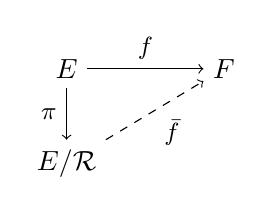
\begin{tikzpicture}[baseline=(current bounding box.center)]
      \node (E)  at (0,1)  {$E$};
      \node (F)  at (2,1)  {$F$};
      \node (Q)  at (0,-0.2) {$E/\mathcal{R}$};
      \draw[->] (E) -- node[above]{\small$f$} (F);
      \draw[->] (E) -- node[left]{\small$\pi$} (Q);
      \draw[->, dashed] (Q) -- node[below right]{\small$\bar{f}$} (F);
    \end{tikzpicture}
  \]
  \textit{est commutatif. De plus, $\bar{f}$ est injective si et seulement si
  $f(x)=f(y) \Rightarrow x\,\mathcal{R}\,y$.}
\end{tcolorbox}

\begin{mdframed}[style=proofbar]
  \textit{Existence et unicité.} On pose $\bar{f}([x]) = f(x)$.
  C'est bien défini : si $[x]=[y]$, alors $x\,\mathcal{R}\,y$, donc $f(x)=f(y)$.
  L'unicité vient de $f = \bar{f}\circ\pi$ : on doit avoir $\bar{f}([x]) = f(x)$.

  \textit{Injectivité ($\Leftarrow$).} Supposons que $f(x)=f(y)\Rightarrow x\,\mathcal{R}\,y$.
  Alors $\bar{f}([x])=\bar{f}([y]) \Rightarrow f(x)=f(y)
  \Rightarrow x\,\mathcal{R}\,y \Rightarrow [x]=[y]$, donc $\bar{f}$ est injective.

  \textit{Injectivité ($\Rightarrow$).} Réciproquement, si $\bar{f}$ est injective
  et $f(x)=f(y)$, alors $\bar{f}([x])=\bar{f}([y])$ (puisque $\bar{f}([z])=f(z)$),
  d'où $[x]=[y]$ par injectivité, c'est-à-dire $x\,\mathcal{R}\,y$. \hfill$\blacksquare$
\end{mdframed}

\decsep{}

%=============================================================
%  § 3 — EXEMPLES FONDAMENTAUX
%=============================================================
\secnum{navyblue}{3}{Exemples fondamentaux}

\begin{mdframed}[style=exbar]
  \textbf{1. Congruences : $\mathbb{Z}/n\mathbb{Z}$.}\enspace%
  \index{congruence}\index{$\mathbb{Z}/n\mathbb{Z}$}
  Sur $\mathbb{Z}$, poser $a \equiv b \pmod{n}$ si $n \mid (b-a)$.
  C'est une relation d'équivalence ; la classe de $a$ est
  $[a] = \{a + kn \mid k \in \mathbb{Z}\}$.
  L'ensemble quotient $\mathbb{Z}/n\mathbb{Z} = \{[0],[1],\ldots,[n-1]\}$
  est un anneau (et même un corps si $n$ est premier).

  \smallskip\noindent
  \textbf{2. Construction de $\mathbb{Q}$.}\enspace%
  \index{nombres rationnels!construction}
  Sur $\mathbb{Z}\times\mathbb{Z}^*$, poser $(a,b)\sim(c,d)$ si $ad = bc$.
  C'est une relation d'équivalence, et
  $\mathbb{Q} = (\mathbb{Z}\times\mathbb{Z}^*)/{\sim}$.
  La classe de $(a,b)$ est notée $\tfrac{a}{b}$.

  \smallskip\noindent
  \textbf{3. Espace vectoriel quotient.}\enspace%
  \index{espace vectoriel quotient}
  Soit $F$ un sous-espace de $E$. On pose $x \sim y$ si $x-y \in F$.
  L'ensemble quotient $E/F$ est naturellement un $\mathbb{K}$-espace vectoriel,
  et lorsque $E$ est de dimension finie, $\dim(E/F) = \dim E - \dim F$
  (propriété du quotient).

  \smallskip\noindent
  \textbf{4. Orbites d'une action de groupe.}\enspace%
  \index{orbite}
  Si un groupe $G$ agit sur $E$, poser $x \sim y$ si $\exists\,g \in G,\, y=g\cdot x$.
  Les classes sont les \emph{orbites} ; $E/{\sim}$ est l'espace des orbites.
\end{mdframed}

\decsep{}

%=============================================================
%  § 4 — APPLICATIONS, PIÈGES, EXERCICES
%=============================================================
\secnum{exgreen}{4}{Applications, pièges et exercices}

\rubriq{Pièges}

\begin{mdframed}[style=cexbar]
  \textbf{Bien-fondé des opérations.}\enspace%
  Pour définir une loi sur $E/\mathcal{R}$, il faut vérifier que l'opération
  ne dépend pas du représentant choisi.
  Exemple piège : sur $\mathbb{Z}$, la relation $a\sim b$ si $|a|=|b|$ est
  une relation d'équivalence, mais $[a]+[b]:=[a+b]$ n'est \emph{pas} bien définie.
  En effet $1\sim{-1}$, donc $[1]=[{-1}]$. Calculons $[1]+[1]$ :
  avec le représentant $1$, on obtient $[1+1]=[2]$ ;
  avec le représentant $-1$, on obtient $[{-1}+1]=[0]$.
  Or $[2]=\{2,-2\}\neq\{0\}=[0]$ : le résultat dépend du choix du représentant.

  \smallskip\noindent
  \textbf{$E/\mathcal{R}$ peut être très grand ou très petit.}\enspace%
  Si $\mathcal{R}$ est l'égalité, $E/\mathcal{R} \cong E$.
  Si $\mathcal{R}$ est la relation grossière ($x\,\mathcal{R}\,y$ toujours), $E/\mathcal{R}$
  est un singleton.
\end{mdframed}

\vspace{6pt}
\exolabel

\begin{mdframed}[style=exobar]
  \begin{enumerate}
    \item Montrer que la relation $\sim$ sur $\mathbb{R}^2$ définie par
          $(x,y)\sim(x',y')$ si $x^2+y^2=x'^2+y'^2$ est une relation
          d'équivalence. Décrire $\mathbb{R}^2/{\sim}$ et la projection canonique.

    \item Soit $f : E \to F$. Montrer que la relation $x\sim_f y \Leftrightarrow f(x)=f(y)$
          est une relation d'équivalence, et que l'application induite
          $\bar{f} : E/{\sim_f} \to F$ est injective. En déduire la décomposition
          canonique $f = \iota \circ \bar{f} \circ \pi$ où $\iota$ est l'injection
          de $\mathrm{Im}(f)$ dans $F$.

    \item Montrer que $\mathbb{Z}/n\mathbb{Z}$ est un corps si et seulement si
          $n$ est premier.

    \item Soit $E = \mathcal{C}([0,1],\mathbb{R})$ et $f \sim g$ si $\int_0^1 f = \int_0^1 g$.
          Montrer que c'est une relation d'équivalence. Décrire $E/{\sim}$.

    \item (Théorème de Noether) Soit $\varphi : G \to H$ un homomorphisme de groupes.
          Montrer que $G/\ker\varphi \cong \mathrm{Im}(\varphi)$.
  \end{enumerate}
\end{mdframed}

\leconfooter{G.\ Cantor (1874) — B.\ Russell (1903) — structures quotient omniprésentes en algèbre}

\clearpage

\chapter{Construction des nombres}

%==============================================================
%  lecons/ensembles/construction_N.tex — Construction de N
%==============================================================

\lecontitle{Construction de \texorpdfstring{$\mathbb{N}$}{N}}{Théorie des ensembles — Axiomes de Peano}

%=============================================================
%  § 1 — MOTIVATION ET AXIOMES DE PEANO
%=============================================================
\secnum{navyblue}{1}{Axiomes de Peano}

\begin{tcolorbox}[thmbox]
  \textbf{Axiomes de Peano (1889).}\enspace%
  \index{Peano (axiomes de)}\index{entiers naturels!axiomes de Peano}
  Il existe un ensemble $\mathbb{N}$ muni d'un élément distingué $0 \in \mathbb{N}$
  et d'une application $S : \mathbb{N} \to \mathbb{N}$ (le \emph{successeur}) vérifiant :
  \begin{enumerate}
    \item[\textbf{P1.}] $0$ n'est le successeur d'aucun entier : $0 \notin \mathrm{Im}(S)$.
    \item[\textbf{P2.}] $S$ est injective : $S(n) = S(m) \Rightarrow n = m$.
    \item[\textbf{P3.}] \textbf{(Récurrence)} Si $A \subseteq \mathbb{N}$ vérifie
      $0 \in A$ et $\forall n \in A,\; S(n) \in A$, alors $A = \mathbb{N}$.
  \end{enumerate}
  On pose $1 = S(0)$, $2 = S(1)$, $3 = S(2)$, etc.
\end{tcolorbox}

\rubriq{Unicité à isomorphisme près}
Si $(\mathbb{N}, 0, S)$ et $(\mathbb{N}', 0', S')$ satisfont tous deux les axiomes
de Peano, il existe un unique isomorphisme $\varphi : \mathbb{N} \to \mathbb{N}'$
tel que $\varphi(0) = 0'$ et $\varphi \circ S = S' \circ \varphi$.
La preuve utilise P3 deux fois : d'abord pour construire $\varphi$ par récurrence,
ensuite pour montrer que c'est une bijection.

\decsep{}

%=============================================================
%  § 2 — ADDITION ET MULTIPLICATION
%=============================================================
\secnum{navyblue}{2}{Définition de l'addition et de la multiplication}

\begin{tcolorbox}[thmbox]
  \textbf{Définition par récurrence.}\enspace%
  \index{entiers naturels!addition}\index{entiers naturels!multiplication}
  On définit $+$ et $\times$ sur $\mathbb{N}$ par :
  \[
    n + 0 = n, \qquad n + S(m) = S(n + m),
  \]
  \[
    n \times 0 = 0, \qquad n \times S(m) = (n \times m) + n.
  \]
  Ces définitions sont légitimes par le \emph{théorème de définition par récurrence} :
  pour toute application $f : \mathbb{N} \to \mathbb{N}$ et tout $a \in \mathbb{N}$,
  il existe une unique suite $(u_n)$ telle que $u_0 = a$ et $u_{S(n)} = f(u_n)$.
\end{tcolorbox}

\begin{mdframed}[style=proofbar]
  On vérifie par récurrence les propriétés algébriques usuelles :
  commutativité, associativité de $+$ et $\times$, distributivité.
  Par exemple, $n + m = m + n$ se montre par double récurrence sur $n$ et $m$.

  \textit{Ordre.} On pose $n \leq m$ si $\exists k \in \mathbb{N},\; m = n + k$.
  C'est un ordre total (P3 garantit la comparabilité) et compatible avec $+$ et $\times$.
  $\blacksquare$
\end{mdframed}

\decsep{}

%=============================================================
%  § 3 — MODÈLE DE VON NEUMANN
%=============================================================
\secnum{navyblue}{3}{Modèle ensembliste — construction de von Neumann}

\begin{tcolorbox}[thmbox]
  \textbf{Construction de von Neumann (dans ZFC).}\enspace%
  \index{von Neumann (construction de)}\index{ZFC}
  On construit $\mathbb{N}$ comme ensemble au sein de la théorie des ensembles
  de Zermelo-Fraenkel avec l'axiome du choix (ZFC) :
  \[
    0 := \emptyset, \quad S(n) := n \cup \{n\}, \quad
    \mathbb{N} := \{0,\, S(0),\, S(S(0)),\, \ldots\}.
  \]
  Explicitement : $0=\emptyset$, $1=\{\emptyset\}$, $2=\{\emptyset,\{\emptyset\}\}$,
  $3=\{\emptyset,\{\emptyset\},\{\emptyset,\{\emptyset\}\}\}$, etc.
  L'existence de $\mathbb{N}$ est garantie par l'\emph{axiome de l'infini}.
\end{tcolorbox}

\rubriq{Signification}
Chaque entier $n$ est identifié à l'ensemble $\{0,1,\ldots,n-1\}$ de ses
prédécesseurs. Ainsi $n \in m \Leftrightarrow n < m$, ce qui donne une
interprétation purement ensembliste de l'ordre.

\decsep{}

%=============================================================
%  § 4 — EXEMPLES, PIÈGES ET EXERCICES
%=============================================================
\secnum{exgreen}{4}{Propriétés, pièges et exercices}

\rubriq{Propriétés fondamentales}

\begin{mdframed}[style=exbar]
  \textbf{1. Principe de bonne fondation.}\enspace%
  \index{bonne fondation}
  Tout sous-ensemble non vide $A \subseteq \mathbb{N}$ admet un plus petit élément.
  \textit{Preuve} : on utilise le lemme de l'ordre discret
  \[
    \forall a,n\in\mathbb{N},\qquad n < a \;\Longrightarrow\; S(n) \leq a,
  \]
  qui exprime qu'aucun entier ne se glisse strictement entre $n$ et $S(n)$
  (il se démontre par récurrence sur $a$ à partir de la définition de $\leq$).
  Soit $A$ non vide et supposons par l'absurde qu'il n'a pas de plus petit
  élément. Posons
  \[
    B = \{n\in\mathbb{N} \mid n \leq a \text{ pour tout } a\in A\}.
  \]
  \emph{Initialisation :} $0 \leq a$ pour tout $a$, donc $0\in B$.
  \emph{Hérédité :} soit $n\in B$, c'est-à-dire $n\leq a$ pour tout $a\in A$.
  Si l'on avait $n\in A$, alors $n$ serait un minorant de $A$ appartenant à $A$,
  donc le plus petit élément de $A$, ce qui est exclu ; ainsi $n\notin A$,
  et pour tout $a\in A$ l'inégalité $n\leq a$ est stricte : $n<a$.
  Le lemme donne alors $S(n)\leq a$ pour tout $a\in A$, donc $S(n)\in B$.
  Par P3, $B = \mathbb{N}$. Comme $A$ est non vide, prenons $a_0\in A$ ;
  alors $S(a_0)\in B$ entraîne $S(a_0)\leq a_0$, ce qui est absurde
  (on a toujours $a_0 < S(a_0)$). $A$ admet donc un plus petit élément.

  \smallskip\noindent
  \textbf{2. Récurrence forte.}\enspace%
  Si $P(n)$ est vraie dès que $P(k)$ est vraie pour tout $k < n$,
  alors $P(n)$ est vraie pour tout $n$. Équivalent à P3 via la bonne fondation.

  \smallskip\noindent
  \textbf{3. Cardinalité.}\enspace%
  $\mathbb{N}$ est infini dénombrable : $|\mathbb{N}| = \aleph_0$.
  Tout sous-ensemble infini de $\mathbb{N}$ est dénombrable.
\end{mdframed}

\vspace{6pt}
\rubriq{Pièges}

\begin{mdframed}[style=cexbar]
  \textbf{$0 \in \mathbb{N}$ ou $0 \notin \mathbb{N}$ ?}\enspace%
  Par convention (ISO 80000-2, Peano), $0 \in \mathbb{N}$. Certains auteurs
  (tradition française classique) posent $\mathbb{N} = \{1,2,3,\ldots\}$.
  Vérifier la convention avant tout raisonnement.

  \smallskip\noindent
  \textbf{Peano au premier ordre : incomplétude et modèles non standard.}\enspace%
  Au premier ordre, l'axiome de récurrence (P3) devient un \emph{schéma} :
  il ne porte que sur les parties de $\mathbb{N}$ définissables par une formule,
  et non sur toutes les parties (catégoricité perdue par rapport à la version
  du second ordre). Deux conséquences classiques en découlent.
  D'une part, par le théorème de \emph{compacité} (ou Löwenheim--Skolem),
  l'arithmétique de Peano admet, à côté du modèle standard $\omega$, des
  \emph{modèles non standard} (contenant des entiers «\,infinis\,») satisfaisant
  exactement les mêmes énoncés du premier ordre.
  D'autre part, par le théorème d'\emph{incomplétude} de Gödel, si PA est
  cohérente il existe des énoncés arithmétiques vrais (dans $\omega$) mais
  non démontrables dans PA.
\end{mdframed}

\vspace{6pt}
\exolabel

\begin{mdframed}[style=exobar]
  \begin{enumerate}
    \item Montrer par récurrence que $\sum_{k=0}^{n} k = n(n+1)/2$.

    \item En utilisant les axiomes de Peano, montrer que la soustraction
          $m - n$ (pour $n \leq m$) est bien définie et unique.

    \item Montrer que $\mathbb{N}$ est le seul modèle à isomorphisme près
          des axiomes de Peano (unicité du modèle standard).

    \item (Division euclidienne) Montrer que pour tous $n,d \in \mathbb{N}$
          avec $d > 0$, il existe des uniques $q, r \in \mathbb{N}$ tels que
          $n = qd + r$ et $0 \leq r < d$.

    \item Montrer que dans la construction de von Neumann, $n \in m
          \Leftrightarrow n \subsetneq m \Leftrightarrow n < m$.
  \end{enumerate}
\end{mdframed}

\leconfooter{G.\ Peano (1889) — J.\ von Neumann (1923) — E.\ Zermelo (1908) \& A.\ Fraenkel (1922)}

\clearpage

%==============================================================
%  lecons/ensembles/construction_Z.tex — Construction de Z
%==============================================================

\lecontitle{Construction de \texorpdfstring{$\mathbb{Z}$}{Z}}{Théorie des ensembles — Extension par différences}

%=============================================================
%  § 1 — MOTIVATION
%=============================================================
\secnum{navyblue}{1}{Motivation — inverser l'addition}

\rubriq{Pourquoi étendre $\mathbb{N}$ ?}
Dans $\mathbb{N}$, l'équation $n + x = m$ n'a pas toujours de solution
(elle n'en a que si $n \leq m$). On veut construire le plus petit anneau
contenant $\mathbb{N}$ dans lequel l'addition est inversible — i.e.\ un
\emph{groupe abélien}.

\begin{tcolorbox}[thmbox]
  \textbf{Idée.}\enspace%
  \index{entiers relatifs!construction}
  Un entier relatif est la «\,différence $m - n$\,» de deux entiers naturels.
  On modélise cela par une paire $(m, n) \in \mathbb{N}^2$ représentant $m - n$,
  avec la relation d'équivalence
  \[
    (m,n) \sim (m', n') \;\iff\; m + n' = m' + n.
  \]
\end{tcolorbox}

\decsep{}

%=============================================================
%  § 2 — CONSTRUCTION FORMELLE
%=============================================================
\secnum{navyblue}{2}{Construction formelle}

\begin{tcolorbox}[thmbox]
  \textbf{Définition.}\enspace%
  On pose $\mathbb{Z} = (\mathbb{N} \times \mathbb{N})/{\sim}$.
  On note $[m,n]$ la classe de $(m,n)$.
  Les lois sont définies par :
  \begin{align*}
    [m,n] + [p,q] &= [m+p,\; n+q], \\
    [m,n] \times [p,q] &= [mp+nq,\; mq+np].
  \end{align*}
  L'élément neutre de $+$ est $[0,0]$, l'opposé de $[m,n]$ est $[n,m]$.
  L'injection $\iota : \mathbb{N} \to \mathbb{Z},\; n \mapsto [n,0]$,
  est un morphisme de semi-anneaux (injection compatible avec $+$ et $\times$ ;
  $\mathbb{N}$ n'étant pas un anneau, on ne parle pas ici d'homomorphisme d'anneaux).
\end{tcolorbox}

\begin{mdframed}[style=proofbar]
  \textit{Bien-fondé de $+$.} Si $(m,n)\sim(m',n')$ et $(p,q)\sim(p',q')$,
  alors $m+n'=m'+n$ et $p+q'=p'+q$. En additionnant :
  $(m+p)+(n'+q') = (m'+p')+(n+q)$, donc $[m+p,n+q] = [m'+p',n'+q']$. $\checkmark$

  \textit{Bien-fondé de $\times$.} Plus délicat. On fixe d'abord $[p,q]$ et l'on
  remplace $(m,n)$ par $(m',n')$ équivalent : en multipliant l'identité
  $m+n'=m'+n$ par $p$ puis par $q$, on obtient
  $(mp+nq)+(m'q+n'p) = (m'p+n'q)+(mq+np)$, c'est-à-dire
  $[mp+nq,\,mq+np]=[m'p+n'q,\,m'q+n'p]$.
  On conclut de même en faisant varier le second facteur.

  \textit{Groupe abélien.} Associativité et commutativité héritées de $\mathbb{N}$.
  Neutre $[0,0]$, opposé $[n,m]$ : $[m,n]+[n,m]=[m+n,n+m]=[0,0]$ (car $m+n=n+m$).

  \textit{Anneau.} La distributivité se vérifie par calcul direct. $\blacksquare$
\end{mdframed}

\decsep{}

%=============================================================
%  § 3 — STRUCTURE ET PROPRIÉTÉS
%=============================================================
\secnum{navyblue}{3}{Structure de $\mathbb{Z}$}

\begin{tcolorbox}[thmbox]
  \textbf{Propriétés de $\mathbb{Z}$.}\enspace%
  \index{entiers relatifs!propriétés}
  \begin{enumerate}
    \item $(\mathbb{Z}, +, \times)$ est un \emph{anneau commutatif intègre}.
    \item $\mathbb{Z}$ est un \emph{anneau principal} : tout idéal de $\mathbb{Z}$
          est de la forme $n\mathbb{Z}$.
    \item L'ordre de $\mathbb{N}$ s'étend : $[m,n] \leq [p,q]
          \Leftrightarrow m+q \leq p+n$ dans $\mathbb{N}$.
          $(\mathbb{Z}, \leq)$ est un ordre total compatible avec $+$.
    \item $\mathrm{Frac}(\mathbb{Z}) = \mathbb{Q}$ (corps des fractions).
  \end{enumerate}
\end{tcolorbox}

\rubriq{Propriétés universelles}

Il faut distinguer deux énoncés de nature différente.

\begin{tcolorbox}[thmbox]
  \textbf{(a) Symétrisation : prolongement des morphismes additifs.}\enspace%
  Soit $(A,+)$ un groupe abélien et $\varphi : \mathbb{N} \to A$ un morphisme
  de monoïdes (i.e.\ $\varphi(m+n)=\varphi(m)+\varphi(n)$ et $\varphi(0)=0_A$).
  Il existe un unique morphisme de groupes $\tilde\varphi : \mathbb{Z} \to A$
  prolongeant $\varphi$, donné par $\tilde\varphi([m,n]) = \varphi(m) - \varphi(n)$.
  C'est la propriété universelle du \emph{groupe des différences} (symétrisation
  du monoïde $(\mathbb{N},+)$) ; elle vaut aussi pour les morphismes de
  semi-anneaux $\mathbb{N}\to A$ vers un anneau $A$, prolongés en morphismes
  d'anneaux.

  \smallskip
  \textbf{(b) Initialité de $\mathbb{Z}$ dans les anneaux unitaires.}\enspace%
  Pour tout anneau unitaire $A$, il existe un \emph{unique} homomorphisme
  d'anneaux unitaires $\chi : \mathbb{Z} \to A$. Autrement dit, $\mathbb{Z}$ est
  l'objet initial de la catégorie des anneaux unitaires.
\end{tcolorbox}

\begin{mdframed}[style=proofbar]
  \textit{Preuve de (b).} Un homomorphisme d'anneaux unitaires $\chi$ doit
  vérifier $\chi(1)=1_A$. Par additivité, $\chi(n)=n\cdot 1_A$ pour tout
  $n\in\mathbb{N}$, puis $\chi(-n)=-(n\cdot 1_A)$ : la valeur de $\chi$ sur tout
  $\mathbb{Z}$ est donc entièrement déterminée par $\chi(1)=1_A$, d'où
  l'unicité. Réciproquement, l'application $\chi(k)=k\cdot 1_A$ est bien définie
  (compatible avec $\sim$) et l'on vérifie que c'est un homomorphisme d'anneaux
  unitaires, d'où l'existence. $\blacksquare$
\end{mdframed}

\decsep{}

%=============================================================
%  § 4 — EXEMPLES, PIÈGES ET EXERCICES
%=============================================================
\secnum{exgreen}{4}{Exemples, pièges et exercices}

\rubriq{Exemples}

\begin{mdframed}[style=exbar]
  \textbf{1. Représentation standard.}\enspace%
  Tout $[m,n]$ est représenté soit par $[k,0]$ (entier $k = m-n \geq 0$)
  soit par $[0,k]$ avec $k \geq 1$ (entier $-k < 0$). On retrouve la
  présentation habituelle.

  \smallskip\noindent
  \textbf{2. Arithmétique.}\enspace%
  $\mathbb{Z}$ est euclidien (division euclidienne), donc principal, donc
  factoriel (décomposition en premiers unique à ordre et signe près).

  \smallskip\noindent
  \textbf{3. Caractéristique.}\enspace%
  $\mathbb{Z}$ est de caractéristique $0$ : $n \cdot 1 = [n,0] \neq [0,0]$
  pour tout $n \geq 1$.
\end{mdframed}

\vspace{6pt}
\rubriq{Pièges}

\begin{mdframed}[style=cexbar]
  \textbf{$\mathbb{Z}$ n'est pas un corps.}\enspace%
  $2 = [2,0]$ n'est pas inversible dans $\mathbb{Z}$ : $[2,0]\cdot[p,q]=[2p,2q]$,
  et $[2p,2q]=[1,0]$ imposerait $2p = 1+2q$, i.e.\ $2(p-q)=1$, impossible
  (membre de gauche pair, membre de droite impair).

  \smallskip\noindent
  \textbf{Divisibilité dans $\mathbb{Z}$ vs $\mathbb{N}$.}\enspace%
  Dans $\mathbb{Z}$, les unités sont $\pm 1$. Les irréductibles (ou premiers)
  se présentent par paires $\{p, -p\}$. Dans $\mathbb{N}$, seuls les $p > 0$
  sont considérés.
\end{mdframed}

\vspace{6pt}
\exolabel

\begin{mdframed}[style=exobar]
  \begin{enumerate}
    \item Montrer que la relation $\sim$ sur $\mathbb{N}^2$ est bien une relation
          d'équivalence.

    \item Montrer que $\mathbb{Z}$ est intègre : si $[m,n]\cdot[p,q]=[0,0]$
          et $[m,n]\neq[0,0]$, alors $[p,q]=[0,0]$.

    \item Montrer que tout idéal de $\mathbb{Z}$ est principal.
          (On utilisera la propriété du bon ordre de $\mathbb{N}$.)

    \item Montrer que $\mathbb{Z}/n\mathbb{Z}$ est un corps si et seulement si
          $n$ est premier.

    \item Soit $\sigma : \mathbb{Z} \to \mathbb{Z}$ un automorphisme d'anneau.
          Montrer que $\sigma = \mathrm{id}$.
  \end{enumerate}
\end{mdframed}

\leconfooter{Construction par paires due à Hamilton, Dedekind et Peano (fin \textsc{xix}\textsuperscript{e} s.) — formalisée dans ZFC au \textsc{xx}\textsuperscript{e} siècle}

\clearpage

%==============================================================
%  lecons/ensembles/construction_Q.tex — Construction de Q
%==============================================================

\lecontitle{Construction de \texorpdfstring{$\mathbb{Q}$}{Q}}{Théorie des ensembles — Corps des fractions de \texorpdfstring{$\mathbb{Z}$}{Z}}

%=============================================================
%  § 1 — MOTIVATION
%=============================================================
\secnum{navyblue}{1}{Motivation — inverser la multiplication}

\rubriq{Pourquoi étendre $\mathbb{Z}$ ?}
Dans $\mathbb{Z}$, l'équation $n \cdot x = m$ n'a de solution entière que
si $n \mid m$. On veut le plus petit corps contenant $\mathbb{Z}$ — on force
la division par tout entier non nul. Ce corps est exactement
$\mathbb{Q} = \mathrm{Frac}(\mathbb{Z})$.

\begin{tcolorbox}[thmbox]
  \textbf{Définition.}\enspace%
  \index{nombres rationnels!construction}\index{corps des fractions}
  Sur $S = \mathbb{Z} \times \mathbb{Z}^*$ (avec $\mathbb{Z}^* = \mathbb{Z}\setminus\{0\}$),
  on pose
  \[
    (a,b) \sim (c,d) \;\iff\; ad = bc.
  \]
  $\mathbb{Q} = S/{\sim}$, muni des lois $\tfrac{a}{b}+\tfrac{c}{d}=\tfrac{ad+bc}{bd}$
  et $\tfrac{a}{b}\cdot\tfrac{c}{d}=\tfrac{ac}{bd}$, est un corps.
\end{tcolorbox}

\decsep{}

%=============================================================
%  § 2 — STRUCTURE ALGÉBRIQUE ET ORDRE
%=============================================================
\secnum{navyblue}{2}{Structure de $\mathbb{Q}$}

\begin{tcolorbox}[thmbox]
  \textbf{Propriétés de $\mathbb{Q}$.}\enspace%
  \index{nombres rationnels!propriétés}
  \begin{enumerate}
    \item $\mathbb{Q}$ est un \emph{corps commutatif} de caractéristique $0$.
    \item L'ordre $\tfrac{a}{b} \leq \tfrac{c}{d}$ (avec $b,d > 0$)
          $\Leftrightarrow ad \leq bc$ fait de $\mathbb{Q}$ un \emph{corps ordonné}.
    \item $\mathbb{Q}$ est \emph{dense} : entre deux rationnels distincts
          il y en a toujours un autre.
    \item $\mathbb{Q}$ est \emph{dénombrable} : il existe une bijection
          $\mathbb{N} \to \mathbb{Q}$ (argument de Cantor — diagonale).
  \end{enumerate}
\end{tcolorbox}

\begin{mdframed}[style=proofbar]
  \textit{Densité.} Si $p < q$ dans $\mathbb{Q}$, alors $p < \tfrac{p+q}{2} < q$. $\checkmark$

  \textit{Dénombrabilité.} On liste les fractions irréductibles $a/b$ avec $b>0$
  en parcourant les diagonales du tableau $\mathbb{Z} \times \mathbb{N}^*$.
  L'image de cette liste est $\mathbb{Q}$, donc $|\mathbb{Q}| \leq |\mathbb{N}|$.
  Comme $\mathbb{N} \hookrightarrow \mathbb{Q}$, on a $|\mathbb{Q}| = \aleph_0$.
  \hfill$\blacksquare$
\end{mdframed}

\rubriq{Représentation unique}
Toute fraction $a/b \in \mathbb{Q}$ s'écrit de façon unique sous la forme
$p/q$ avec $\pgcd(p,q) = 1$ et $q > 0$ (\emph{fraction irréductible}).

\decsep{}

%=============================================================
%  § 3 — INCOMPLÉTUDE DE Q
%=============================================================
\secnum{navyblue}{3}{Incomplétude de $\mathbb{Q}$}

\begin{tcolorbox}[thmbox]
  \textbf{Théorème ($\sqrt{2} \notin \mathbb{Q}$).}\enspace%
  \index{irrationalité de $\sqrt{2}$}
  Il n'existe pas de rationnel $x$ tel que $x^2 = 2$.
\end{tcolorbox}

\begin{mdframed}[style=proofbar]
  Supposons $x = p/q$ irréductible vérifiant $p^2 = 2q^2$.
  Alors $2 \mid p^2$, donc $2 \mid p$ (car $2$ est premier). Écrivons $p = 2k$.
  Alors $4k^2 = 2q^2$, soit $2k^2 = q^2$, donc $2 \mid q$. Contradiction avec
  $\pgcd(p,q) = 1$. \hfill$\blacksquare$
\end{mdframed}

\rubriq{Conséquence : $\mathbb{Q}$ n'est pas complet}
La suite $(x_n)$ définie par $x_0 = 1$ et $x_{n+1} = \tfrac{x_n}{2} + \tfrac{1}{x_n}$
est de Cauchy dans $\mathbb{Q}$ mais converge vers $\sqrt{2} \notin \mathbb{Q}$.
Cette incomplétude motive la construction de $\mathbb{R}$.

\decsep{}

%=============================================================
%  § 4 — EXEMPLES, PIÈGES ET EXERCICES
%=============================================================
\secnum{exgreen}{4}{Exemples, pièges et exercices}

\noindent{\bfseries\color{navyblue} Exemples.}

\begin{mdframed}[style=exbar]
  \textbf{1. Corps premier.}\enspace%
  \index{corps premier}
  $\mathbb{Q}$ est le \emph{corps premier} de caractéristique $0$ : tout corps
  de caractéristique $0$ contient un sous-corps isomorphe à $\mathbb{Q}$.

  \smallskip\noindent
  \textbf{2. Approximation.}\enspace%
  Théorème de Dirichlet : pour tout $\alpha \in \mathbb{R}$ et $N \geq 1$,
  il existe $p/q$ avec $1 \leq q \leq N$ et $|\alpha - p/q| \leq 1/(qN)$.
  Ainsi $\mathbb{Q}$ est dense dans $\mathbb{R}$ pour la topologie usuelle.

  \smallskip\noindent
  \textbf{3. Topologie.}\enspace%
  Muni de la valeur absolue usuelle, $\mathbb{Q}$ est un espace métrique.
  Sa complétion est $\mathbb{R}$. Muni de la valeur absolue $p$-adique
  $|\cdot|_p$, sa complétion est $\mathbb{Q}_p$.
\end{mdframed}

\vspace{6pt}
\noindent{\bfseries\color{counterred} Pièges.}

\begin{mdframed}[style=cexbar]
  \textbf{Dense $\neq$ complet.}\enspace%
  $\mathbb{Q}$ est dense dans $\mathbb{R}$ (tout réel est limite de rationnels),
  mais pas complet : des suites de Cauchy rationnelles peuvent converger vers
  des irrationnels.

  \smallskip\noindent
  \textbf{Corps ordonné $\neq$ archimédien.}\enspace%
  Tout corps ordonné n'est pas archimédien. Mais $\mathbb{Q}$ l'est :
  pour tout $x \in \mathbb{Q}^+$, il existe $n \in \mathbb{N}$ tel que $n > x$.
\end{mdframed}

\vspace{6pt}
\noindent{\bfseries\color{goldaccent} Exercices.}

\begin{mdframed}[style=exobar]
  \begin{enumerate}
    \item Montrer que $\sqrt{3}$, $\sqrt{5}$ et $\sqrt{2}+\sqrt{3}$ sont irrationnels.

    \item Montrer que $\mathbb{Q}$ est dénombrable en utilisant le théorème
          de Schröder-Bernstein.

    \item Montrer que tout corps ordonné archimédien se plonge dans $\mathbb{R}$.

    \item Montrer que $\mathbb{Q}$ n'admet pas d'extension algébrique finie
          de degré $1$ autre que lui-même (i.e.\ tout polynôme irréductible
          sur $\mathbb{Q}$ de degré $\geq 2$ n'a pas de racine dans $\mathbb{Q}$).
          Donner un exemple de degré $2$.

    \item Soit $\alpha \in \mathbb{R}$ algébrique sur $\mathbb{Q}$.
          Montrer que $\mathbb{Q}(\alpha)$ est dénombrable.
  \end{enumerate}
\end{mdframed}

\leconfooter{Euclide (irrationnalité de $\sqrt{2}$, \textit{ca.} $-$300) — G.\ Cantor (dénombrabilité, 1874)}

\clearpage

%==============================================================
%  lecons/ensembles/construction_R.tex — Construction de R
%==============================================================

\lecontitle{Construction de \texorpdfstring{$\mathbb{R}$}{R}}{Théorie des ensembles — Complétion de \texorpdfstring{$\mathbb{Q}$}{Q}}

%=============================================================
%  § 1 — DEUX APPROCHES
%=============================================================
\secnum{navyblue}{1}{Deux constructions classiques}

\rubriq{Le problème}
$\mathbb{Q}$ est dense mais incomplet. On veut le compléter : obtenir un corps
ordonné archimédien \emph{complet}, c'est-à-dire dans lequel toute suite de
Cauchy converge. Il existe deux méthodes standards.

\begin{tcolorbox}[thmbox]
  \textbf{Construction A — Coupures de Dedekind (1872).}\enspace%
  \index{coupures de Dedekind}\index{réels!construction par coupures}
  Une \emph{coupure} est un couple $(L, U)$ de sous-ensembles non vides de $\mathbb{Q}$
  vérifiant :
  \begin{enumerate}
    \item $L \cup U = \mathbb{Q}$ et $L \cap U = \emptyset$.
    \item $L$ est un \emph{segment initial} : $x \in L$ et $y < x \Rightarrow y \in L$.
    \item $L$ n'a pas de maximum.
  \end{enumerate}
  On pose $\mathbb{R} = \{\,L\mid (L,U)\text{ coupure}\,\}$. L'ensemble $U$ est alors
  entièrement déterminé par $L = \mathbb{Q}\setminus U$ : dans toute la suite, on
  \emph{identifie la coupure à son segment initial $L$}, de sorte que tous les
  énoncés ci-dessous ($\subseteq$, $\sup = \bigcup$, $\hat q = \{r < q\}$) portent
  sur des ensembles de rationnels.
\end{tcolorbox}

\begin{tcolorbox}[thmbox]
  \textbf{Construction B — Suites de Cauchy (Cantor, 1872).}\enspace%
  \index{réels!construction par suites de Cauchy}
  Soit $\mathcal{C}$ l'ensemble des suites de Cauchy dans $\mathbb{Q}$.
  On pose $(a_n) \sim (b_n)$ si $a_n - b_n \to 0$. Alors
  \[
    \mathbb{R} = \mathcal{C}/{\sim}
  \]
  muni des lois terme à terme est un corps complet.
\end{tcolorbox}

\decsep{}

%=============================================================
%  § 2 — CONSTRUCTION PAR COUPURES
%=============================================================
\secnum{navyblue}{2}{Détail de la construction de Dedekind}

\begin{mdframed}[style=proofbar]
  \textit{Ordre.} On pose $\alpha \leq \beta$ si $\alpha \subseteq \beta$ (en tant que
  sous-ensembles de $\mathbb{Q}$). C'est un ordre total sur $\mathbb{R}$.

  \textit{Borne supérieure.} Si $A \subseteq \mathbb{R}$ est non vide et majoré,
  alors $\sup A = \bigcup_{\alpha \in A} \alpha$ est une coupure et c'est le plus
  petit majorant de $A$. C'est la propriété de la \emph{borne supérieure}.

  \textit{Addition.} $\alpha + \beta = \{a + b \mid a \in \alpha,\; b \in \beta\}$.
  On vérifie que c'est une coupure, et que les axiomes de groupe abélien sont satisfaits.

  \textit{Multiplication.} Plus délicate, car il faut gérer les signes.
  Pour $\alpha, \beta > 0$ (c'est-à-dire $\alpha, \beta \supsetneq \hat 0$), on pose
  \[
    \alpha \cdot \beta = \mathbb{Q}^- \cup \{\, ab \mid a \in \alpha,\ b \in \beta,\ a, b > 0 \,\},
  \]
  soit tous les rationnels $\leq 0$ réunis aux produits de représentants strictement
  positifs des deux coupures (on vérifie que l'ensemble obtenu est une coupure~:
  fermé vers le bas, distinct de $\mathbb{Q}$ car majoré par tout produit de
  majorants, et sans maximum). On étend ensuite à $\alpha, \beta$ quelconques par les règles des signes :
  $\alpha\cdot 0 = 0$, et pour $\alpha < 0$ ou $\beta < 0$ on pose
  $\alpha\cdot\beta = \pm\bigl(|\alpha|\cdot|\beta|\bigr)$ selon le signe attendu,
  avec $|\gamma| = \max(\gamma, -\gamma)$.

  \textit{Plongement de $\mathbb{Q}$.} À $q \in \mathbb{Q}$ on associe la coupure
  $\hat{q} = \{r \in \mathbb{Q} \mid r < q\}$. \hfill$\blacksquare$
\end{mdframed}

\decsep{}

%=============================================================
%  § 3 — CONSTRUCTION PAR SUITES DE CAUCHY
%=============================================================
\secnum{navyblue}{3}{Détail de la construction de Cantor}

\rubriq{Étape 1 — L'anneau $\mathcal{C}$}

\begin{mdframed}[style=proofbar]
  Soit $\mathcal{C} = \{(a_n)_{n\in\mathbb{N}} \in \mathbb{Q}^{\mathbb{N}} \mid (a_n)
  \text{ est de Cauchy}\}$ l'ensemble des suites de Cauchy à valeurs dans $\mathbb{Q}$.
  On vérifie que $\mathcal{C}$ est un sous-anneau de $\mathbb{Q}^{\mathbb{N}}$ :

  \begin{itemize}
    \item Si $(a_n)$ et $(b_n)$ sont de Cauchy, alors $(a_n + b_n)$ l'est
    (inégalité triangulaire : $|(a_n+b_n)-(a_m+b_m)| \leq |a_n-a_m|+|b_n-b_m|$).
    \item Si $(a_n)$ et $(b_n)$ sont de Cauchy, elles sont bornées
    ($|a_n| \leq M$, $|b_n| \leq N$). Alors
    $|a_nb_n - a_mb_m| \leq M|b_n-b_m| + N|a_n-a_m| \to 0$,
    donc $(a_nb_n)$ est de Cauchy.
  \end{itemize}
  \hfill$\blacksquare$
\end{mdframed}

\rubriq{Étape 2 — La relation d'équivalence}

\begin{mdframed}[style=proofbar]
  On définit $(a_n) \sim (b_n)$ si $a_n - b_n \to 0$ dans $\mathbb{Q}$.
  C'est bien une relation d'équivalence (réflexivité et symétrie sont immédiates ;
  transitivité : $a_n - c_n = (a_n - b_n) + (b_n - c_n) \to 0$).

  \textit{Compatibilité avec les lois.}
  Si $(a_n)\sim(a_n')$ et $(b_n)\sim(b_n')$, alors
  $(a_n+b_n)-(a_n'+b_n') = (a_n-a_n')+(b_n-b_n') \to 0$ ($+$ bien fondé).
  Pour $\times$ : $(a_nb_n - a_n'b_n') = a_n(b_n-b_n') + b_n'(a_n-a_n') \to 0$
  car $(a_n)$ et $(b_n')$ sont bornées (étant de Cauchy) tandis que
  $(b_n-b_n'),(a_n-a_n')\to 0$ ($\times$ bien fondé).
  \hfill$\blacksquare$
\end{mdframed}

\rubriq{Étape 3 — $\mathbb{R} = \mathcal{C}/{\sim}$ est un corps}

\begin{mdframed}[style=proofbar]
  On note $[(a_n)]$ la classe d'équivalence de $(a_n)$, avec lois
  $[(a_n)]+[(b_n)] = [(a_n+b_n)]$ et $[(a_n)]\cdot[(b_n)]=[(a_nb_n)]$.

  \textit{Neutre additif :} $[(0)]$ (suite constante nulle).
  \textit{Opposé de $[(a_n)]$ :} $[(-a_n)]$.

  \textit{Inverse multiplicatif.}
  Soit $[(a_n)] \neq [(0)]$, i.e.\ $(a_n) \not\to 0$.
  Alors il existe $\varepsilon > 0$ et $N \in \mathbb{N}$ tels que
  $|a_n| > \varepsilon$ pour tout $n \geq N$.
  (En effet, $(a_n)\not\to 0$ fournit un $\varepsilon>0$ et une infinité d'indices
  $m$ tels que $|a_m| > 2\varepsilon$ ; comme $(a_n)$ est de Cauchy, $|a_n-a_m|<\varepsilon$
  pour $n,m\geq N$, d'où $|a_n| \geq |a_m| - |a_n-a_m| > \varepsilon$ dès $n\geq N$.)
  On pose
  \[
    b_n =
    \begin{cases}
      1 & \text{si } n < N, \\
      1/a_n & \text{si } n \geq N.
    \end{cases}
  \]
  Pour $n, m \geq N$ : $|b_n - b_m| = \dfrac{|a_n - a_m|}{|a_n||a_m|}
  \leq \dfrac{|a_n-a_m|}{\varepsilon^2} \to 0$,
  donc $(b_n) \in \mathcal{C}$.
  Et $a_nb_n = 1$ pour $n \geq N$, donc $[(a_n)]\cdot[(b_n)] = [(1)]$.
  Ainsi tout élément non nul est inversible : $\mathbb{R}$ est un corps.
  \hfill$\blacksquare$
\end{mdframed}

\rubriq{Étape 4 — Ordre et plongement de $\mathbb{Q}$}

\begin{mdframed}[style=proofbar]
  \textit{Ordre.} On dit que $[(a_n)] > 0$ s'il existe $\varepsilon > 0$
  et $N$ tels que $a_n > \varepsilon$ pour tout $n \geq N$.
  (Bien fondé : si $(a_n)\sim(a_n')$ et $a_n > \varepsilon$ pour $n\geq N$,
  alors $|a_n-a_n'| < \varepsilon/2$ pour $n$ assez grand, donc $a_n' > \varepsilon/2$.)
  On pose $\alpha \leq \beta$ si $\beta - \alpha \geq 0$.
  C'est un ordre total compatible avec les lois.

  \textit{Plongement.} $\iota : \mathbb{Q} \to \mathbb{R},\; q \mapsto [(q,q,q,\ldots)]$
  est un homomorphisme de corps ordonné injectif.
  On identifie $\mathbb{Q}$ à son image.
  \hfill$\blacksquare$
\end{mdframed}

\rubriq{Étape 5 — $\mathbb{R}$ est complet}

\begin{mdframed}[style=proofbar]
  \textbf{Théorème.}\enspace Toute suite de Cauchy dans $\mathbb{R}$ converge.

  \medskip
  Soit $(\alpha^{(k)})_{k\geq 1}$ une suite de Cauchy dans $\mathbb{R}$,
  avec $\alpha^{(k)} = [(a_n^{(k)})_{n\geq 0}]$.

  \textit{Extraction d'une suite diagonale.}
  Pour chaque $k$, $(a_n^{(k)})$ est de Cauchy dans $\mathbb{Q}$, donc
  il existe $N_k \in \mathbb{N}$ tel que
  \[
    n, m \geq N_k \;\Rightarrow\; |a_n^{(k)} - a_m^{(k)}| < \tfrac{1}{k}.
  \]
  On pose $c_k = a_{N_k}^{(k)} \in \mathbb{Q}$.

  \textit{$(c_k)$ est de Cauchy dans $\mathbb{Q}$.}
  Pour $k, \ell$ grands, $|\alpha^{(k)} - \alpha^{(\ell)}| < \varepsilon/3$
  (hypothèse Cauchy sur $(\alpha^{(k)})$), et $|\alpha^{(k)} - \iota(c_k)| \leq 1/k$
  (par construction de $c_k$). L'inégalité triangulaire donne $|c_k - c_\ell| < \varepsilon$
  pour $k, \ell$ assez grands.

  \textit{Convergence.} Posons $\lambda = [(c_k)] \in \mathbb{R}$.
  Alors $|\alpha^{(k)} - \lambda| \leq |\alpha^{(k)} - \iota(c_k)| + |\iota(c_k) - \lambda| \to 0$,
  car $|\alpha^{(k)} - \iota(c_k)| \leq 1/k \to 0$ et $|\iota(c_k) - \lambda|\to 0$
  puisque $\lambda$ est précisément la classe de la suite de Cauchy $(c_k)$.
  \hfill$\blacksquare$
\end{mdframed}

\decsep{}

%=============================================================
%  § 4 — PROPRIÉTÉS FONDAMENTALES
%=============================================================
\secnum{navyblue}{4}{Caractérisation axiomatique de $\mathbb{R}$}

\begin{tcolorbox}[thmbox]
  \textbf{Théorème (unicité).}\enspace%
  \index{réels!axiomatique}
  À isomorphisme de corps ordonnés près, il existe un \emph{unique} corps ordonné
  complet archimédien. C'est $\mathbb{R}$.

  \medskip
  \textbf{Propriétés équivalentes à la complétude.}
  Les énoncés suivants sont tous équivalents pour un corps ordonné archimédien :
  \begin{enumerate}
    \item Toute suite de Cauchy converge.
    \item Tout sous-ensemble non vide majoré admet une borne supérieure.
    \item Toute suite de segments emboîtés $[a_n, b_n] \supseteq [a_{n+1}, b_{n+1}]$
          avec $b_n-a_n\to 0$ admet un point commun (segments emboîtés).
    \item Toute suite croissante majorée converge (théorème de la limite monotone).
  \end{enumerate}
\end{tcolorbox}

\rubriq{Non dénombrabilité}

\begin{mdframed}[style=proofbar]
  \textbf{Théorème de Cantor.}\enspace%
  \index{non dénombrabilité de $\mathbb{R}$}
  $\mathbb{R}$ n'est pas dénombrable : $|\mathbb{R}| = 2^{\aleph_0} =: \mathfrak{c}$
  (puissance du continu).

  \textit{Preuve (argument diagonal).}
  Il suffit de montrer que le segment $[0,1]$ n'est pas dénombrable, ce qui
  entraîne \emph{a fortiori} la non-dénombrabilité de $\mathbb{R}$. Supposons donc
  $[0,1]$ dénombrable : $[0,1] = \{x_1, x_2, \ldots\}$.
  Construisons $y \in [0,1]$ différent de chaque $x_n$ : si le $n$-ième chiffre
  décimal de $x_n$ est $d$, on pose le $n$-ième chiffre décimal de $y$ égal à
  $5$ si $d \neq 5$, et $6$ sinon. En n'utilisant que les chiffres $5$ et $6$,
  $y$ admet un développement décimal unique (pas de phénomène $0{,}999\ldots=1$),
  et $y \in [0,1]$ mais $y \neq x_n$ pour tout $n$ (ils diffèrent au rang $n$) :
  contradiction. Cet argument n'établit que la non-dénombrabilité ; l'égalité
  $|\mathbb{R}| = 2^{\aleph_0}$ s'obtient ensuite en comparant $\mathbb{R}$ et
  $\{0,1\}^{\mathbb{N}}$ via les développements binaires, puis en appliquant le
  théorème de Cantor--Bernstein.
  \hfill$\blacksquare$
\end{mdframed}

\decsep{}

%=============================================================
%  § 5 — EXEMPLES, PIÈGES ET EXERCICES
%=============================================================
\secnum{exgreen}{5}{Exemples, pièges et exercices}

\rubriq{Exemples}

\begin{mdframed}[style=exbar]
  \textbf{1. Nombres algébriques et transcendants.}\enspace%
  \index{nombre transcendant}
  Les réels algébriques sur $\mathbb{Q}$ forment un sous-corps dénombrable de $\mathbb{R}$.
  Donc «\,la plupart\,» des réels sont transcendants ($e$ par Hermite 1873,
  $\pi$ par Lindemann 1882).

  \smallskip\noindent
  \textbf{2. Mesure de Lebesgue.}\enspace%
  $\mathbb{Q}$ est de mesure nulle dans $\mathbb{R}$ : $\lambda(\mathbb{Q}) = 0$.
  Cela illustre que densité et mesure positive sont des notions indépendantes.

  \smallskip\noindent
  \textbf{3. Topologie.}\enspace%
  $\mathbb{R}$ est localement compact, $\sigma$-compact, connexe, et localement
  connexe. C'est, à homéomorphisme près, l'unique variété topologique connexe
  de dimension $1$, sans bord, non compacte et à base dénombrable.
\end{mdframed}

\vspace{6pt}
\rubriq{Pièges}

\begin{mdframed}[style=cexbar]
  \textbf{Les deux constructions donnent le même objet.}\enspace%
  Les constructions de Dedekind et de Cantor-Cauchy produisent des corps
  ordonnés complets archimédiens, donc isomorphes par unicité.
  La «\,meilleure\,» construction dépend du contexte.

  \smallskip\noindent
  \textbf{Hypothèse du continu.}\enspace%
  On a $\aleph_0 < \mathfrak{c}$, mais la question de savoir s'il existe
  un cardinal strictement entre $\aleph_0$ et $\mathfrak{c}$ est
  \emph{indécidable} dans ZFC (Cohen, 1963).
\end{mdframed}

\vspace{6pt}
\exolabel

\begin{mdframed}[style=exobar]
  \begin{enumerate}
    \item Vérifier que la borne supérieure de coupures $\sup A = \bigcup_{\alpha\in A}\alpha$
          est bien une coupure de Dedekind.

    \item Montrer que les quatre propriétés de complétude (Cauchy, borne sup,
          intervalles emboîtés, suite monotone majorée) sont équivalentes dans
          un corps ordonné archimédien.

    \item Montrer que $\mathbb{R}\setminus\mathbb{Q}$ est non dénombrable.

    \item Montrer que la complétion de $(\mathbb{Q}, |\cdot|_p)$ pour la valeur
          absolue $p$-adique est $\mathbb{Q}_p$, qui n'est \emph{pas} archimédien.

    \item (Théorème de Baire) Montrer que $\mathbb{R}$ n'est pas réunion
          dénombrable d'ensembles fermés d'intérieur vide.
  \end{enumerate}
\end{mdframed}

\leconfooter{R.\ Dedekind (1872) — G.\ Cantor (1872) — unicité due à E.\ Huntington (1903)}

\clearpage

%==============================================================
%  lecons/ensembles/construction_C.tex — Construction de C
%==============================================================

\lecontitle{Construction de \texorpdfstring{$\mathbb{C}$}{C}}{Théorie des ensembles — Clôture algébrique de \texorpdfstring{$\mathbb{R}$}{R}}

%=============================================================
%  § 1 — MOTIVATION
%=============================================================
\secnum{navyblue}{1}{Motivation — fermer algébriquement $\mathbb{R}$}

\rubriq{Le problème}
Dans $\mathbb{R}$, le polynôme $X^2 + 1$ n'a pas de racine. On veut étendre
$\mathbb{R}$ en un corps algébriquement clos, c'est-à-dire dans lequel
tout polynôme non constant a au moins une racine.

\begin{tcolorbox}[thmbox]
  \textbf{Construction algébrique.}\enspace%
  \index{nombres complexes!construction}\index{corps algébriquement clos}
  On construit $\mathbb{C}\cong\mathbb{R}[X]/(X^2+1)$ en réalisant cet isomorphisme
  de corps sur l'ensemble $\mathbb{R}^2$ (à ne pas confondre avec l'anneau-produit
  $\mathbb{R}\times\mathbb{R}$ qui n'est pas un corps), muni des lois :
  \begin{align*}
    (a,b) + (c,d) &= (a+c,\; b+d), \\
    (a,b) \times (c,d) &= (ac-bd,\; ad+bc).
  \end{align*}
  On note $i = (0,1)$, de sorte que $i^2 = (-1, 0)$, identifié à $-1$.
  L'injection $\mathbb{R} \hookrightarrow \mathbb{C},\; a \mapsto (a,0)$,
  est un homomorphisme de corps.
\end{tcolorbox}

\begin{significationintuitive}
  Le quotient $\mathbb{R}[X]/(X^2+1)$ consiste à manipuler les polynômes réels
  \emph{modulo} la relation $X^2+1 = 0$, c'est-à-dire en convenant que $X^2 = -1$.
  Tout reste de division par $X^2+1$ est de degré $\leq 1$, donc de la forme
  $a + bX$ : on retrouve ainsi le plan $\mathbb{R}^2$, et la classe de $X$ joue le
  rôle de $i$. La table de multiplication $(a,b)\times(c,d) = (ac-bd,\,ad+bc)$
  n'est rien d'autre que le produit $(a+bX)(c+dX) = ac + (ad+bc)X + bd\,X^2$ où
  l'on remplace $X^2$ par $-1$.
\end{significationintuitive}

\decsep{}

%=============================================================
%  § 2 — STRUCTURE ALGÉBRIQUE
%=============================================================
\secnum{navyblue}{2}{$\mathbb{C}$ est un corps}

\begin{mdframed}[style=proofbar]
  \textit{Corps.} Les axiomes de groupe abélien pour $+$ sont immédiats. La
  multiplication est commutative, associative et distributive sur $+$ : cela se
  vérifie par calcul direct à partir des propriétés correspondantes de $\mathbb{R}$,
  l'élément neutre étant $(1,0)$. Pour l'inverse multiplicatif de
  $(a,b) \neq (0,0)$ :
  \[
    {(a,b)}^{-1} = \left(\frac{a}{a^2+b^2},\; \frac{-b}{a^2+b^2}\right).
  \]
  En effet $(a,b)\cdot(a,-b) = (a^2+b^2, 0)$ s'identifie au réel $a^2+b^2 \neq 0$
  (car $a^2+b^2 > 0$ dès que $(a,b)\neq(0,0)$), d'où la formule ci-dessus en
  divisant par ce réel.

  \textit{Dimension.} $\mathbb{C}$ est un $\mathbb{R}$-espace vectoriel de dimension $2$,
  de base $(1, i)$. Tout $z \in \mathbb{C}$ s'écrit $z = a + ib$ avec $a,b\in\mathbb{R}$.
  $\blacksquare$
\end{mdframed}

\begin{tcolorbox}[thmbox]
  \textbf{Propriétés fondamentales.}\enspace%
  \index{nombres complexes!module}\index{nombres complexes!conjugué}
  Pour $z = a+ib$, on définit :
  \[
    \bar{z} = a - ib \quad \text{(conjugué)}, \qquad
    |z| = \sqrt{a^2+b^2} \quad \text{(module)}.
  \]
  On a $z \bar{z} = |z|^2$, $|zw| = |z||w|$, et $|z+w| \leq |z|+|w|$
  (inégalité triangulaire).
  La forme polaire est $z = |z|e^{i\theta}$ avec $\theta = \arg z$.
\end{tcolorbox}

\decsep{}

%=============================================================
%  § 3 — THÉORÈME FONDAMENTAL DE L'ALGÈBRE
%=============================================================
\secnum{navyblue}{3}{Théorème fondamental de l'algèbre}

\begin{tcolorbox}[thmbox]
  \textbf{Théorème (d'Alembert–Gauss).}\enspace%
  \index{théorème fondamental de l'algèbre}
  $\mathbb{C}$ est \emph{algébriquement clos} : tout polynôme
  $P \in \mathbb{C}[X]$ de degré $n \geq 1$ admet au moins une racine dans
  $\mathbb{C}$.

  \medskip
  \emph{Corollaire.} Par récurrence sur le degré (en factorisant un facteur
  $(X-a)$ à chaque étape), tout $P$ de degré $n \geq 1$ admet alors
  \emph{exactement} $n$ racines dans $\mathbb{C}$, comptées avec multiplicités.

  \medskip
  Comme $\mathbb{C}$ est algébriquement clos et que l'extension
  $\mathbb{C}/\mathbb{R}$ est algébrique (de degré $2$), $\mathbb{C}$ est la
  \emph{clôture algébrique} de $\mathbb{R}$. À ne pas confondre avec la définition
  d'algébriquement clos elle-même, qui exprime que toute extension algébrique de
  $\mathbb{C}$ est triviale (égale à $\mathbb{C}$).
\end{tcolorbox}

\begin{mdframed}[style=proofbar]
  \textit{Esquisse (preuve topologique).}
  Quitte à diviser $P$ par son coefficient dominant (ce qui ne change pas ses
  racines), on suppose $P$ \emph{unitaire}. Supposons que $P$ (de degré
  $n\geq 1$) n'ait aucune racine. Alors
  $z \mapsto P(z)/|P(z)|$ est définie et continue sur $\mathbb{C}$ tout entier,
  à valeurs dans le cercle $\mathbb{S}^1$. Sa restriction au cercle de rayon $R$
  est donc une boucle, dont l'indice (élément de $\pi_1(\mathbb{S}^1)\cong\mathbb{Z}$)
  ne dépend pas de $R$~— la boucle varie continûment avec $R$ et son indice,
  entier, est donc constant : en faisant $R \to 0$, la boucle se contracte
  en la constante $P(0)/|P(0)|$, donc cet indice est nul. Mais pour $|z|\to\infty$
  on a $P(z)/|P(z)| \sim z^n/|z|^n$, qui s'enroule $n$ fois autour de l'origine,
  d'indice $n$. Comme l'indice est un entier invariant par homotopie, on aurait
  $0 = n$ : contradiction puisque $n \geq 1$. \hfill$\blacksquare$
\end{mdframed}

\rubriq{Conséquence : classification des corps}
Toute extension algébrique finie de $\mathbb{R}$ est soit $\mathbb{R}$ soit $\mathbb{C}$
(extension de degré $2$). Il n'existe pas d'extension algébrique de $\mathbb{R}$
de degré $3$ ou plus.

\decsep{}

%=============================================================
%  § 4 — EXEMPLES, PIÈGES ET EXERCICES
%=============================================================
\secnum{exgreen}{4}{Exemples, pièges et exercices}

\rubriq{Exemples}

\begin{mdframed}[style=exbar]
  \textbf{1. Formule d'Euler.}\enspace%
  \index{formule d'Euler}
  $e^{i\theta} = \cos\theta + i\sin\theta$. En particulier,
  $e^{i\pi} + 1 = 0$ (identité d'Euler).

  \smallskip\noindent
  \textbf{2. Racines $n$-ièmes de l'unité.}\enspace%
  \index{racines de l'unité}
  Les solutions de $z^n = 1$ sont $\omega_k = e^{2ik\pi/n}$ pour $k = 0, \ldots, n-1$.
  Elles forment le groupe cyclique $\mu_n \cong \mathbb{Z}/n\mathbb{Z}$.

  \smallskip\noindent
  \textbf{3. Transformée de Fourier.}\enspace%
  L'utilisation de $\mathbb{C}$ est fondamentale en analyse harmonique :
  $\hat{f}(\xi) = \int_{\mathbb{R}} f(x) e^{-2\pi i x\xi}\,\mathrm{d}x$.
\end{mdframed}

\vspace{6pt}
\rubriq{Pièges}

\begin{mdframed}[style=cexbar]
  \textbf{$\mathbb{C}$ n'est pas un corps ordonné.}\enspace%
  Il n'existe aucun ordre total sur $\mathbb{C}$ compatible avec $+$ et $\times$.
  En effet, dans un corps ordonné tout carré est $\geq 0$, donc on aurait
  $i^2 = -1 \geq 0$, en contradiction avec $-1 < 0$.

  \smallskip\noindent
  \textbf{Pas de clôture algébrique canonique.}\enspace%
  La clôture algébrique de $\mathbb{Q}$ (les nombres algébriques $\bar{\mathbb{Q}}$)
  n'est pas $\mathbb{C}$ entier — c'est un sous-corps strict. Par ailleurs, la
  clôture algébrique est unique \emph{à isomorphisme près}, mais cet isomorphisme
  n'est ni unique ni canonique : le groupe $\mathrm{Aut}(\bar{\mathbb{Q}}/\mathbb{Q})$
  est immense.
\end{mdframed}

\vspace{6pt}
\exolabel

\begin{mdframed}[style=exobar]
  \begin{enumerate}
    \item Montrer que $\mathbb{R}[X]/(X^2+1)$ est bien un corps, et que
          $(X^2+1)$ est un idéal maximal de $\mathbb{R}[X]$.

    \item Trouver toutes les racines carrées de $3 + 4i$.

    \item Montrer que tout automorphisme de corps de $\mathbb{C}$
          fixant $\mathbb{R}$ est soit l'identité, soit la conjugaison.

    \item Factoriser $X^4 + 4$ dans $\mathbb{R}[X]$, puis dans $\mathbb{C}[X]$.

    \item (Théorème de Liouville) Montrer qu'une fonction entière bornée
          est constante, et en déduire le théorème fondamental de l'algèbre.
  \end{enumerate}
\end{mdframed}

\leconfooter{R.\ Descartes (1637) — C.\ F.\ Gauss (1799, thèse) — J.\ le Rond d'Alembert (1746)}

\clearpage

%==============================================================
%  lecons/ensembles/construction_H.tex — Construction de H
%==============================================================

\lecontitle{Construction de \texorpdfstring{$\mathbb{H}$}{H}}{Théorie des ensembles — Quaternions de Hamilton}

%=============================================================
%  § 1 — MOTIVATION ET DÉFINITION
%=============================================================
\secnum{navyblue}{1}{Définition des quaternions}

\rubriq{Contexte historique}
Hamilton cherchait (1843) à étendre $\mathbb{C}$ pour représenter les rotations
de l'espace $\mathbb{R}^3$. Après des années à tenter une structure en
dimension $3$, il découvrit que la dimension $4$ est nécessaire, en renonçant
à la commutativité de la multiplication.

\begin{tcolorbox}[thmbox]
  \textbf{Définition.}\enspace%
  \index{quaternions!définition}\index{Hamilton (quaternions de)}
  L'algèbre des \emph{quaternions} est
  \[
    \mathbb{H} = \{a + bi + cj + dk \mid a,b,c,d \in \mathbb{R}\}
  \]
  munie de l'addition composante par composante et de la multiplication
  déterminée par les relations de Hamilton :
  \[
    i^2 = j^2 = k^2 = ijk = -1.
  \]
  Ces relations imposent :
  $ij = k,\ ji = -k,\ jk = i,\ kj = -i,\ ki = j,\ ik = -j$.
\end{tcolorbox}

\decsep{}

%=============================================================
%  § 2 — STRUCTURE ALGÉBRIQUE
%=============================================================
\secnum{navyblue}{2}{$\mathbb{H}$ est un corps gauche}

\begin{tcolorbox}[thmbox]
  \textbf{Propriétés fondamentales.}\enspace%
  \index{quaternions!norme}\index{quaternions!conjugué}\index{corps gauche}
  Pour $q = a + bi + cj + dk \in \mathbb{H}$, on définit :
  \[
    \bar{q} = a - bi - cj - dk \quad \text{(conjugué)},
    \qquad
    |q|^2 = q\bar{q} = a^2+b^2+c^2+d^2 \quad \text{(norme au carré)}.
  \]
  \begin{enumerate}
    \item $\overline{pq} = \bar{q}\bar{p}$ pour tous $p,q \in \mathbb{H}$.
    \item $|pq| = |p||q|$ (multiplicativité de la norme).
    \item Pour $q \neq 0$ : $q^{-1} = \bar{q}/|q|^2$.
    \item $(\mathbb{H}, +, \times)$ est un \emph{corps gauche} (division ring) :
          tous les axiomes d'un corps sauf la commutativité de $\times$.
  \end{enumerate}
\end{tcolorbox}

\begin{mdframed}[style=proofbar]
  \textit{Inverse.} $q \cdot \bar{q} = |q|^2 \in \mathbb{R}_+^*$, donc
  $q \cdot (\bar{q}/|q|^2) = 1$. De même $(\bar{q}/|q|^2) \cdot q = 1$,
  ce qui donne bien un inverse à gauche et à droite.

  \textit{Associativité.} Vérification directe (fastidieuse mais mécanique) :
  on vérifie les $64$ triplets de base ${\{1,i,j,k\}}^3$.

  \textit{Non-commutativité.} $ij = k \neq -k = ji$.
  \hfill$\blacksquare$
\end{mdframed}

\rubriq{Construction matricielle}

\begin{mdframed}[style=proofbar]
  $\mathbb{H}$ est isomorphe (comme algèbre réelle) au sous-anneau de
  $\mathcal{M}_2(\mathbb{C})$ :
  \[
    a + bi + cj + dk \;\longmapsto\;
    \begin{pmatrix} a+bi & c+di \\ -(c-di) & a-bi \end{pmatrix}
    =
    \begin{pmatrix} a+bi & c+di \\ -\overline{c+di} & \overline{a+bi} \end{pmatrix}.
  \]
  Pour établir que l'application est un morphisme d'algèbres, il suffit de
  vérifier que les images de $1,i,j,k$ satisfont les relations de Hamilton, ce
  qui se ramène à un calcul sur quatre matrices. Le déterminant de l'image vaut
  $|q|^2$ : les quaternions de norme $1$ correspondent donc exactement aux
  matrices de $\mathrm{SU}(2)$.
  \hfill$\blacksquare$
\end{mdframed}

\decsep{}

%=============================================================
%  § 3 — ROTATIONS ET GÉOMÉTRIE
%=============================================================
\secnum{navyblue}{3}{Quaternions et rotations de $\mathbb{R}^3$}

\begin{tcolorbox}[thmbox]
  \textbf{Théorème (Hamilton–Rodrigues).}\enspace%
  \index{quaternions!rotations}\index{Rodrigues (formule de)}
  Soit $\mathbf{n}$ un vecteur unitaire de $\mathbb{R}^3$ et $\theta \in \mathbb{R}$.
  Le quaternion unitaire $q = \cos(\theta/2) + \sin(\theta/2)(n_1 i + n_2 j + n_3 k)$
  représente la rotation d'axe $\mathbf{n}$ et d'angle $\theta$ via :
  \[
    \mathbf{v} \;\longmapsto\; q\,\mathbf{v}\,\bar{q}
  \]
  où $\mathbf{v}$ est identifié au quaternion pur $v_1 i + v_2 j + v_3 k$.
\end{tcolorbox}

\begin{significationintuitive}
  Appliquée à un quaternion pur, la conjugaison $\mathbf{v}\mapsto q\mathbf{v}\bar{q}$
  redonne un quaternion pur et préserve la norme : c'est donc bien une isométrie
  de $\mathbb{R}^3$, et l'on vérifie qu'elle fixe l'axe $\mathbf{n}$. L'apparition
  de l'angle moitié $\theta/2$ vient de ce que $q$ agit \emph{deux fois}, une fois
  à gauche par $q$ et une fois à droite par $\bar{q}$. C'est aussi pourquoi $q$ et
  $-q$ produisent la même rotation, puisque $(-q)\mathbf{v}\,\overline{(-q)} = q\mathbf{v}\bar{q}$ :
  on retrouve ainsi le noyau $\{\pm 1\}$ du recouvrement ci-dessous.
\end{significationintuitive}

\rubriq{Double recouvrement de $\mathrm{SO}(3)$}
L'application $q \mapsto (v \mapsto qv\bar{q})$ est un homomorphisme de groupes
surjectif $\mathrm{Sp}(1) \to \mathrm{SO}(3)$ (où $\mathrm{Sp}(1)$ désigne les
quaternions unitaires), de noyau $\{\pm 1\}$.
Ainsi $\mathrm{SO}(3) \cong \mathrm{Sp}(1)/\{\pm 1\} \cong \mathrm{SU}(2)/\{\pm I\}$.

\decsep{}

%=============================================================
%  § 4 — THÉORÈME DE FROBENIUS ET EXERCICES
%=============================================================
\secnum{exgreen}{4}{Classification, pièges et exercices}

\rubriq{Théorème de classification}

\begin{mdframed}[style=exbar]
  \textbf{Théorème de Frobenius (1877).}\enspace%
  \index{Frobenius (théorème de)}
  Les seules algèbres \emph{associatives} à division de dimension finie sur
  $\mathbb{R}$ sont : $\mathbb{R}$, $\mathbb{C}$ et $\mathbb{H}$.

  \smallskip\noindent
  \textbf{Octonions $\mathbb{O}$.}\enspace%
  \index{octonions}
  En abandonnant aussi l'associativité, on obtient les \emph{octonions} $\mathbb{O}$
  (dimension $8$). Par le théorème de Hurwitz (1898), les seules algèbres
  normées sur $\mathbb{R}$ \emph{dont la norme est multiplicative}
  ($\lVert xy\rVert = \lVert x\rVert\,\lVert y\rVert$) sont
  $\mathbb{R}, \mathbb{C}, \mathbb{H}, \mathbb{O}$
  (dimensions $1, 2, 4, 8$).
\end{mdframed}

\vspace{6pt}
\rubriq{Pièges}

\begin{mdframed}[style=cexbar]
  \textbf{$\mathbb{H}$ n'est pas commutatif.}\enspace%
  Ne pas développer comme dans un anneau commutatif :
  $(p+q)^2 = p^2 + pq + qp + q^2$, et en général $pq + qp \neq 2pq$.
  De même $(pq)^2 \neq p^2q^2$ en général : $(ij)^2 = k^2 = -1$
  alors que $i^2j^2 = (-1)(-1) = 1$.

  \smallskip\noindent
  \textbf{Pas de polynômes bien définis.}\enspace%
  Dans $\mathbb{H}[X]$, l'équation $X^2 + 1 = 0$ a une infinité de solutions :
  tous les quaternions purs unitaires $bi+cj+dk$ avec $b^2+c^2+d^2=1$.
  L'algèbre des polynômes est délicate en non-commutatif.
\end{mdframed}

\vspace{6pt}
\exolabel


\begin{mdframed}[style=exobar]
  \begin{enumerate}
    \item Vérifier les relations $ij=k$, $jk=i$, $ki=j$ à partir de $i^2=j^2=k^2=ijk=-1$.

    \item Montrer que $|pq|=|p||q|$ pour tous $p,q\in\mathbb{H}$.

    \item Montrer que les quaternions unitaires $\mathrm{Sp}(1) = \{q \in \mathbb{H} \mid |q|=1\}$
          forment un groupe (homéomorphe à $\mathbb{S}^3$).

    \item Calculer la rotation correspondant au quaternion $q = \tfrac{1}{2}(1+i+j+k)$.
          Quel est son axe et son angle ?

    \item Montrer que le centre de $\mathbb{H}$ est $\mathbb{R}$, i.e.\ que
          seuls les scalaires commutent avec tous les quaternions.
  \end{enumerate}
\end{mdframed}

\leconfooter{W.\ R.\ Hamilton (16 octobre 1843) — G.\ Frobenius (1877) — A.\ Hurwitz (1898)}

\clearpage

\chapter{Groupes, anneaux et corps}

%==============================================================
%  lecons/algebre/groupes.tex — Groupes
%==============================================================

\lecontitle{Groupes}{Algèbre — Structures avec une loi de groupe}

%=============================================================
%  § 1 — DÉFINITION ET EXEMPLES
%=============================================================
\secnum{navyblue}{1}{Définition et premiers exemples}

\begin{tcolorbox}[thmbox]
  \textbf{Définition.}\enspace%
  \index{groupe}\index{groupe abélien}
  Un \emph{groupe} est un ensemble $G$ muni d'une loi interne $\cdot$ vérifiant :
  \begin{enumerate}
    \item[\textbf{G1.}] \textbf{Associativité :} $(a\cdot b)\cdot c = a\cdot(b\cdot c)$.
    \item[\textbf{G2.}] \textbf{Élément neutre :} $\exists e \in G,\; \forall a,\; e\cdot a = a\cdot e = a$.
    \item[\textbf{G3.}] \textbf{Symétrique :} $\forall a \in G,\; \exists a^{-1} \in G,\;
          a\cdot a^{-1} = a^{-1}\cdot a = e$.
  \end{enumerate}
  Si de plus $a \cdot b = b \cdot a$ pour tous $a, b$, le groupe est dit
  \emph{abélien} (ou \emph{commutatif}) ; on note alors la loi $+$ et le neutre $0$.
\end{tcolorbox}

\rubriq{Exemples fondamentaux}

\begin{mdframed}[style=exbar]
  \textbf{1. Groupes additifs.}\enspace%
  $(\mathbb{Z},+)$, $(\mathbb{Q},+)$, $(\mathbb{R},+)$, $(\mathbb{C},+)$
  sont des groupes abéliens. $(\mathbb{N},+)$ n'est \emph{pas} un groupe
  (pas d'opposé).

  \smallskip\noindent
  \textbf{2. Groupes multiplicatifs.}\enspace%
  $(\mathbb{Q}^*,\times)$, $(\mathbb{R}^*,\times)$, $(\mathbb{C}^*,\times)$,
  $(\mathbb{U},\times)$ (racines de l'unité) sont abéliens.

  \smallskip\noindent
  \textbf{3. Groupe symétrique $\mathfrak{S}_n$.}\enspace%
  \index{groupe symétrique}
  L'ensemble des bijections de $\{1,\ldots,n\}$ dans lui-même, muni de la
  composition, est un groupe d'ordre $n!$. Non abélien pour $n \geq 3$.

  \smallskip\noindent
  \textbf{4. Groupe linéaire $\mathrm{GL}_n(\mathbb{K})$.}\enspace%
  \index{groupe linéaire}
  Les matrices inversibles de $\mathcal{M}_n(\mathbb{K})$, muni du produit matriciel.
  Non abélien pour $n \geq 2$.

  \smallskip\noindent
  \textbf{5. $\mathbb{Z}/n\mathbb{Z}$.}\enspace%
  \index{$\mathbb{Z}/n\mathbb{Z}$}
  Groupe abélien d'ordre $n$, cyclique, engendré par $[1]$.
\end{mdframed}

\decsep{}

%=============================================================
%  § 2 — SOUS-GROUPES ET MORPHISMES
%=============================================================
\secnum{navyblue}{2}{Sous-groupes et morphismes}

\begin{tcolorbox}[thmbox]
  \textbf{Définition.}\enspace%
  \index{sous-groupe}\index{morphisme de groupes}
  Une partie $H \subseteq G$ est un \emph{sous-groupe} si
  $e \in H$ et $\forall a,b \in H,\; ab^{-1} \in H$.

  \medskip
  Une application $\varphi : G \to H$ est un \emph{morphisme de groupes} si
  $\varphi(ab) = \varphi(a)\varphi(b)$ pour tous $a,b \in G$.
  Son \emph{noyau}\index{noyau d'un morphisme} est $\ker\varphi = \varphi^{-1}(\{e_H\})$,
  son \emph{image} est $\mathrm{Im}(\varphi) = \varphi(G)$.
\end{tcolorbox}

\begin{mdframed}[style=proofbar]
  \textit{$\ker\varphi$ est un sous-groupe de $G$.}
  $e_G \in \ker\varphi$ car $\varphi(e_G) = e_H$.
  Si $a,b \in \ker\varphi$ : $\varphi(ab^{-1}) = \varphi(a)\varphi(b)^{-1} = e_H$,
  donc $ab^{-1} \in \ker\varphi$. $\checkmark$

  \textit{$\mathrm{Im}(\varphi)$ est un sous-groupe de $H$.} Analogue. $\checkmark$

  \textit{$\varphi$ est injective ssi $\ker\varphi = \{e_G\}$.}
  Si $\ker\varphi = \{e_G\}$ et $\varphi(a)=\varphi(b)$, alors
  $\varphi(ab^{-1}) = e_H$, donc $ab^{-1} = e_G$, soit $a = b$.
  \hfill$\blacksquare$
\end{mdframed}

\begin{tcolorbox}[thmbox]
  \textbf{Sous-groupes de $\mathbb{Z}$.}\enspace%
  \index{sous-groupes de $\mathbb{Z}$}
  Tout sous-groupe de $(\mathbb{Z},+)$ est de la forme $n\mathbb{Z}$
  pour un unique $n \in \mathbb{N}$.
\end{tcolorbox}

\begin{mdframed}[style=proofbar]
  Soit $H \leq \mathbb{Z}$. Si $H = \{0\}$, $H = 0\mathbb{Z}$. Sinon,
  $H$ contient un entier $> 0$ (car si $a \in H$, $a\neq 0$, alors $|a| = \pm a \in H$).
  Soit $n = \min(H \cap \mathbb{N}^*)$. Clairement $n\mathbb{Z} \subseteq H$.
  Pour tout $h \in H$, la division euclidienne donne $h = qn + r$ avec $0 \leq r < n$ ;
  or $r = h - qn \in H$, donc $r = 0$ par minimalité de $n$. Ainsi $H = n\mathbb{Z}$.
  \hfill$\blacksquare$
\end{mdframed}

\decsep{}

%=============================================================
%  § 3 — THÉORÈME DE LAGRANGE ET GROUPE QUOTIENT
%=============================================================
\secnum{navyblue}{3}{Théorème de Lagrange et premier théorème d'isomorphisme}

\begin{tcolorbox}[thmbox]
  \textbf{Théorème de Lagrange.}\enspace%
  \index{Lagrange (théorème de)}
  \textit{Soit $G$ un groupe fini et $H$ un sous-groupe de $G$. Alors
  $|H|$ divise $|G|$, et $|G| = |H| \cdot [G:H]$, où $[G:H]$ est le
  nombre de classes à gauche de $H$ dans $G$.}

  \medskip
  \textbf{Corollaire.}\enspace%
  L'\emph{ordre}\index{ordre d'un élément} d'un élément $a \in G$
  (le plus petit $k \geq 1$ tel que $a^k = e$) divise $|G|$.
  En particulier, $a^{|G|} = e$ pour tout $a \in G$.
\end{tcolorbox}

\begin{mdframed}[style=proofbar]
  \textit{Les classes à gauche $aH = \{ah \mid h \in H\}$ forment une partition de $G$}
  (cf.\ relation d'équivalence $a \sim b \Leftrightarrow a^{-1}b \in H$).
  Chaque classe a cardinal $|H|$ (la bijection $h \mapsto ah$ est de $H$ vers $aH$).
  Donc $|G| = |H| \cdot |\{$classes$\}| = |H| \cdot [G:H]$. \hfill$\blacksquare$
\end{mdframed}

\begin{tcolorbox}[thmbox]
  \textbf{Sous-groupe distingué et groupe quotient.}\enspace%
  \index{sous-groupe distingué}\index{groupe quotient}
  $H$ est \emph{distingué} dans $G$ (noté $H \trianglelefteq G$) si
  $gHg^{-1} = H$ pour tout $g \in G$.
  Dans ce cas, l'ensemble des classes $G/H$ est muni d'une structure de groupe
  par $(aH)(bH) = (ab)H$.

  \medskip
  \textbf{Premier théorème d'isomorphisme.}\enspace%
  \index{isomorphisme (premier théorème d')}
  Si $\varphi : G \to H$ est un morphisme de groupes, alors $\ker\varphi \trianglelefteq G$
  et
  \[
    G/\ker\varphi \;\cong\; \mathrm{Im}(\varphi).
  \]
\end{tcolorbox}

\begin{mdframed}[style=proofbar]
  \textit{Bien-fondé de la loi sur $G/H$.}
  Si $a' \in aH$ et $b' \in bH$, alors $a'b' = (ah_1)(bh_2) = ab(b^{-1}h_1b)h_2$.
  Comme $H \trianglelefteq G$, $b^{-1}h_1b \in H$, donc $a'b' \in abH$. $\checkmark$

  \textit{Isomorphisme.}
  L'application $\bar\varphi : G/\ker\varphi \to \mathrm{Im}(\varphi),\; a\ker\varphi \mapsto \varphi(a)$
  est bien définie, injective (si $\varphi(a)=e_H$ alors $a\in\ker\varphi$),
  surjective sur $\mathrm{Im}(\varphi)$, et c'est un morphisme. \hfill$\blacksquare$
\end{mdframed}

\decsep{}

%=============================================================
%  § 4 — GROUPES CYCLIQUES, PIÈGES, EXERCICES
%=============================================================
\secnum{exgreen}{4}{Groupes cycliques, pièges et exercices}

\noindent{\bfseries\color{navyblue} Groupes cycliques.}

\begin{mdframed}[style=exbar]
  \textbf{Définition.}\enspace%
  \index{groupe cyclique}
  $G$ est \emph{cyclique} s'il existe $g \in G$ (un \emph{générateur}) tel que
  $G = \langle g \rangle = \{g^n \mid n \in \mathbb{Z}\}$.

  \smallskip\noindent
  \textbf{Classification.}\enspace%
  Tout groupe cyclique est isomorphe à $\mathbb{Z}$ (si infini) ou $\mathbb{Z}/n\mathbb{Z}$
  (si d'ordre $n$). Les générateurs de $\mathbb{Z}/n\mathbb{Z}$ sont les $[k]$ avec
  $\pgcd(k,n)=1$ : il y en a $\varphi(n)$ (indicatrice d'Euler).

  \smallskip\noindent
  \textbf{Petit théorème de Fermat.}\enspace%
  \index{Fermat (petit théorème de)}
  Pour $p$ premier et $a \not\equiv 0 \pmod{p}$ : $a^{p-1} \equiv 1 \pmod{p}$.
  Preuve : $(\mathbb{Z}/p\mathbb{Z})^*$ est un groupe d'ordre $p-1$, donc $a^{p-1}=e$.
\end{mdframed}

\vspace{6pt}
\noindent{\bfseries\color{counterred} Pièges.}

\begin{mdframed}[style=cexbar]
  \textbf{Un sous-groupe n'est pas toujours distingué.}\enspace%
  Dans $\mathfrak{S}_3$, $H = \{e, (12)\}$ est un sous-groupe mais pas distingué :
  $(123)(12)(123)^{-1} = (23) \notin H$.

  \smallskip\noindent
  \textbf{Tout groupe d'ordre premier est cyclique.}\enspace%
  Si $|G| = p$ premier, tout $g \neq e$ engendre $G$ (car $|\langle g\rangle|$
  divise $p$, donc vaut $p$). En particulier $G \cong \mathbb{Z}/p\mathbb{Z}$.

  \smallskip\noindent
  \textbf{Réciproque de Lagrange fausse.}\enspace%
  Si $d \mid |G|$, il n'existe pas forcément un sous-groupe d'ordre $d$.
  Contre-exemple : $A_4$ (d'ordre $12$) n'a pas de sous-groupe d'ordre $6$.
\end{mdframed}

\vspace{6pt}
\exolabel

\begin{mdframed}[style=exobar]
  \begin{enumerate}
    \item Montrer que l'intersection d'une famille de sous-groupes de $G$
          est un sous-groupe de $G$.

    \item Montrer que $\mathfrak{S}_n$ est engendré par les transpositions,
          et que le signe $\varepsilon : \mathfrak{S}_n \to \{+1,-1\}$
          est un morphisme de groupes surjectif.

    \item Montrer que tout groupe d'ordre $p^2$ (p premier) est abélien.
          (\textit{Hint :} considérer le centre $Z(G)$.)

    \item Soit $G$ fini et $H, K$ deux sous-groupes de $G$. Montrer que
          $|HK| = |H||K|/|H\cap K|$.

    \item (Théorème de Cayley) Montrer que tout groupe fini $G$ est
          isomorphe à un sous-groupe de $\mathfrak{S}_{|G|}$.
  \end{enumerate}
\end{mdframed}

\leconfooter{É.\ Galois (1830) — A.\ Cayley (1854) — L.\ Sylow (1872)}

\clearpage

%==============================================================
%  lecons/algebre/sous_groupes_additifs.tex — Sous-groupes additifs de R
%==============================================================

\lecontitle{Sous-groupes additifs de \texorpdfstring{$\mathbb{R}$}{R}}{Algèbre \& topologie — Dichotomie monogène ou dense}

%=============================================================
%  § 1 — ÉNONCÉ ET SIGNIFICATION
%=============================================================
\secnum{navyblue}{1}{Énoncé et signification}

\begin{tcolorbox}[thmbox]
  \textbf{Théorème (dichotomie).}\enspace%
  \index{sous-groupe additif de $\mathbb{R}$}\index{sous-groupe!monogène}\index{sous-groupe!dense}
  Soit $G$ un sous-groupe de $(\mathbb{R},+)$. Alors l'une exactement des deux
  situations suivantes se produit :
  \begin{enumerate}
    \item \textbf{cas monogène :} il existe un unique réel $a \geq 0$ tel que
          \[
            G = a\mathbb{Z} = \{\,na : n \in \mathbb{Z}\,\} ;
          \]
    \item \textbf{cas dense :} $G$ est dense dans $\mathbb{R}$.
  \end{enumerate}
  Plus précisément, lorsque $G \neq \{0\}$ on pose
  $a = \inf\bigl(G \cap \,]0,+\infty[\,\bigr)$ : on est dans le cas monogène
  lorsque $a > 0$, et dans le cas dense lorsque $a = 0$. Le cas $G = \{0\}$ est
  monogène de générateur $a = 0$ (la convention $\inf(\emptyset) = +\infty$ sert
  seulement à exprimer qu'alors $G$ n'a aucun élément $> 0$).
\end{tcolorbox}

\begin{significationintuitive}
Un sous-groupe additif de $\mathbb{R}$ ne peut pas être « à moitié discret ».
Soit ses éléments strictement positifs admettent un plus petit représentant $a$,
et alors tout le groupe est constitué des multiples entiers de ce « pas »~; soit
ils s'accumulent en $0$, et la translation par ces éléments arbitrairement petits
permet d'atteindre n'importe quel réel d'aussi près que l'on veut. La frontière
entre les deux mondes est nette : il n'existe pas d'intermédiaire.
\end{significationintuitive}

\decsep{}

%=============================================================
%  § 2 — DÉMONSTRATION
%=============================================================
\secnum{navyblue}{2}{Démonstration}

\begin{ideepreuve}
On mesure la « finesse » du groupe par $a = \inf(G \cap \,]0,+\infty[)$.
Si $a > 0$, on montre d'abord que cette borne inférieure est atteinte
($a \in G$) à l'aide d'un argument de différence de deux éléments trop proches,
puis la division euclidienne réelle donne $G = a\mathbb{Z}$. Si $a = 0$, le
groupe contient des éléments positifs aussi petits que voulu, et leurs multiples
quadrillent $\mathbb{R}$ : c'est la densité.
\end{ideepreuve}

\rubriq{Preuve}

\begin{mdframed}[style=proofbar]
  \textit{Le cas trivial.}\enspace
  Si $G = \{0\}$, alors $G = 0\cdot\mathbb{Z}$ : c'est le cas monogène avec $a=0$.
  On suppose désormais $G \neq \{0\}$. Si $x \in G \setminus \{0\}$, alors $-x \in G$
  (sous-groupe), donc $|x| \in G \cap \,]0,+\infty[$ : cet ensemble est non vide
  et minoré par $0$, sa borne inférieure
  \[
    a = \inf\bigl(G \cap \,]0,+\infty[\,\bigr) \geq 0
  \]
  est bien définie.

  \medskip
  \textit{Cas $a > 0$ : montrons d'abord $a \in G$.}\enspace
  Supposons par l'absurde $a \notin G$. Par définition de la borne inférieure
  appliquée à $\varepsilon = a$, il existe $g \in G$ avec $a < g < 2a$ (l'inégalité
  est stricte à gauche car $a \notin G$). Appliquée ensuite à $\varepsilon = g - a > 0$,
  elle fournit $h \in G$ avec $a < h < g$. Alors
  \[
    g - h \in G \quad\text{et}\quad 0 < g - h < g - a < a,
  \]
  donc $g - h \in G \cap \,]0,+\infty[$ tout en vérifiant $g - h < a$, ce qui
  contredit le fait que $a$ minore $G \cap \,]0,+\infty[$. Donc $a \in G$.

  \medskip
  \textit{Cas $a > 0$ : conclusion $G = a\mathbb{Z}$.}\enspace
  Comme $a \in G$, on a $a\mathbb{Z} \subseteq G$. Réciproquement, soit $x \in G$.
  La division euclidienne réelle donne $q = \lfloor x/a \rfloor \in \mathbb{Z}$ et
  un reste $r = x - qa$ avec $0 \leq r < a$. Or $r = x - qa \in G$ (car $x \in G$
  et $qa \in G$), et $a$ est le plus petit élément strictement positif de $G$ ;
  l'encadrement $0 \leq r < a$ force $r = 0$. Ainsi $x = qa \in a\mathbb{Z}$, d'où
  $G = a\mathbb{Z}$.

  \medskip
  \textit{Cas $a = 0$ : densité.}\enspace
  Soit $x \in \mathbb{R}$ et $\varepsilon > 0$. Puisque $\inf(G \cap \,]0,+\infty[) = 0$,
  il existe $g \in G$ avec $0 < g < \varepsilon$. Posons $n = \lfloor x/g \rfloor \in \mathbb{Z}$,
  de sorte que $ng \leq x < (n+1)g$, donc
  \[
    |x - ng| < g < \varepsilon, \qquad ng \in G.
  \]
  Tout réel est donc limite d'éléments de $G$ : $G$ est dense dans $\mathbb{R}$.

  \medskip
  \textit{Exclusivité et unicité.}\enspace
  Si $a > 0$, l'intervalle $]0,a[$ ne rencontre pas $G$, donc $G$ n'est pas dense :
  les deux cas s'excluent. Enfin, si $a\mathbb{Z} = b\mathbb{Z}$ avec $a,b \geq 0$ :
  si $a = 0$, alors $b\mathbb{Z} = \{0\}$, donc $b = 0$ ; si $a > 0$, alors $a$ est
  le plus petit élément strictement positif de $a\mathbb{Z} = b\mathbb{Z}$, et $b$
  l'est aussi, d'où $a = b$ :
  le générateur positif est unique. \hfill$\blacksquare$
\end{mdframed}

\decsep{}

%=============================================================
%  § 3 — APPLICATION : LE GROUPE $\mathbb{Z} + \alpha\mathbb{Z}$
%=============================================================
\secnum{navyblue}{3}{Application : le groupe \texorpdfstring{$\mathbb{Z}+\alpha\mathbb{Z}$}{Z + aZ}}

\begin{tcolorbox}[thmbox]
  \textbf{Théorème (critère d'irrationalité).}\enspace%
  \index{groupe!$\mathbb{Z}+\alpha\mathbb{Z}$}\index{Kronecker (théorème de)}
  Soit $\alpha \in \mathbb{R}$ et $G = \mathbb{Z} + \alpha\mathbb{Z}
  = \{\,m + n\alpha : (m,n) \in \mathbb{Z}^2\,\}$. Alors :
  \[
    G \text{ est dense dans } \mathbb{R} \iff \alpha \notin \mathbb{Q}.
  \]
  De façon équivalente, la suite des parties fractionnaires $(\{n\alpha\})_{n\in\mathbb{N}}$
  est dense dans $[0,1]$ si et seulement si $\alpha$ est irrationnel.
\end{tcolorbox}

\rubriq{Preuve}

\begin{mdframed}[style=proofbar]
  $G$ est un sous-groupe de $(\mathbb{R},+)$, on lui applique la dichotomie.

  \smallskip\noindent
  \textit{Si $\alpha = p/q \in \mathbb{Q}$} (fraction irréductible, $q \geq 1$),
  alors $m + n\alpha = (mq + np)/q \in \tfrac{1}{q}\mathbb{Z}$. Réciproquement,
  comme $\pgcd(p,q) = 1$, le théorème de Bézout fournit $u,v \in \mathbb{Z}$ avec
  $up + vq = 1$, d'où $\tfrac1q = u\alpha + v \in G$ et donc
  $\tfrac1q\mathbb{Z} \subseteq G$ ; ainsi $G = \tfrac1q\mathbb{Z}$ est monogène,
  \emph{non} dense.

  \smallskip\noindent
  \textit{Si $\alpha \notin \mathbb{Q}$}, supposons $G$ monogène, $G = a\mathbb{Z}$
  avec $a > 0$. Comme $1 \in G$ et $\alpha \in G$, il existe $k, \ell \in \mathbb{Z}$
  avec $1 = ka$ et $\alpha = \ell a$. Alors $a = 1/k$ puis $\alpha = \ell/k \in \mathbb{Q}$,
  contradiction. Le cas monogène est donc exclu : $G$ est dense.

  \smallskip\noindent
  Enfin, chaque $\{n\alpha\} = n\alpha - \lfloor n\alpha\rfloor$ appartient à
  $G \cap [0,1[$ (car $n\alpha \in G$ et $\lfloor n\alpha\rfloor \in \mathbb{Z}
  \subseteq G$). Si $\alpha = p/q \in \mathbb{Q}$, cet ensemble
  $G \cap [0,1[\, = \tfrac1q\mathbb{Z} \cap [0,1[$ est fini : la suite n'est pas
  dense. Si $\alpha \notin \mathbb{Q}$, soit $\varepsilon \in \,]0,1[$ ; par
  densité de $G$, il existe $g = m + r\alpha \in G$ avec $0 < g < \varepsilon$,
  et $r \neq 0$ (sinon $g = m$ serait un entier de $]0,1[$). Si $r > 0$, alors
  $\{r\alpha\} = g$ et, pour tout $k \in \mathbb{N}$ tel que $kg < 1$, on a
  $\{kr\alpha\} = kg$ : ces points quadrillent $[0,1]$ avec un pas $g < \varepsilon$.
  Si $r < 0$, alors $\{(-r)\alpha\} = 1 - g$ et $\{k(-r)\alpha\} = 1 - kg$ tant
  que $kg < 1$ : même quadrillage, parcouru en sens inverse. Dans les deux cas,
  tout point de $[0,1]$ est à distance $< \varepsilon$ d'un $\{n\alpha\}$ avec
  $n \in \mathbb{N}$ : la suite $(\{n\alpha\})_{n\in\mathbb{N}}$ est dense dans
  $[0,1]$.
  \hfill$\blacksquare$
\end{mdframed}

\rubriq{Exemples}

\begin{mdframed}[style=exbar]
  \textbf{1. Pas régulier.}\enspace%
  $G = \frac{1}{2}\mathbb{Z} = \{\ldots,-1,-\tfrac12,0,\tfrac12,1,\ldots\}$ est
  monogène de générateur $a = \tfrac12$.

  \smallskip\noindent
  \textbf{2. $\mathbb{Q}$ est dense.}\enspace%
  $\mathbb{Q}$ est un sous-groupe de $(\mathbb{R},+)$ contenant des éléments
  positifs arbitrairement petits ($\tfrac1n \to 0$) : $a = 0$, il est dense
  --- ce que l'on savait déjà, ici relu par la dichotomie.

  \smallskip\noindent
  \textbf{3. Densité de $(\cos n)_{n\in\mathbb{N}}$.}\enspace%
  \index{densité!de $(\cos n)$}
  Comme $\pi \notin \mathbb{Q}$ (irrationalité admise), $2\pi$ est irrationnel, donc
  $\mathbb{Z} + 2\pi\mathbb{Z}$ est dense dans $\mathbb{R}$ : les entiers $n$ pris
  modulo $2\pi$ sont denses dans $[0,2\pi[$. Par continuité du cosinus,
  $\{\cos n : n \in \mathbb{N}\}$ est dense dans $[-1,1]$.
\end{mdframed}

\rubriq{Contre-exemples et points de vigilance}

\begin{mdframed}[style=cexbar]
  \textbf{$\mathbb{N}$ n'est pas un sous-groupe.}\enspace%
  $\mathbb{N}$ est discret mais n'est \emph{pas} de la forme $a\mathbb{Z}$ : la
  dichotomie ne s'y applique pas, faute d'opposés. L'hypothèse « sous-groupe »
  est essentielle.

  \smallskip\noindent
  \textbf{Dense $\neq$ égal à $\mathbb{R}$.}\enspace%
  $\mathbb{Q}$ et $\mathbb{Z}+\sqrt2\,\mathbb{Z}$ sont denses dans $\mathbb{R}$
  sans être $\mathbb{R}$ tout entier : la densité est une propriété topologique,
  pas une égalité ensembliste.

  \smallskip\noindent
  \textbf{Pas d'intermédiaire.}\enspace%
  Il n'existe pas de sous-groupe de $\mathbb{R}$ qui soit à la fois non monogène
  et non dense : un sous-groupe additif de $\mathbb{R}$ est soit fermé (et alors
  $\{0\}$, $a\mathbb{Z}$ ou $\mathbb{R}$), soit dense.
\end{mdframed}

\exolabel

\begin{mdframed}[style=exobar]
  \begin{enumerate}
    \item Montrer que tout sous-groupe \emph{fermé} de $(\mathbb{R},+)$ est
          $\{0\}$, $a\mathbb{Z}$ ($a>0$), ou $\mathbb{R}$.
    \item Soit $\alpha$ irrationnel. Montrer que $\{m + n\alpha : m,n \in \mathbb{Z}\}$
          rencontre tout intervalle ouvert non vide.
    \item En déduire que $(\sin n)_{n \in \mathbb{N}}$ est dense dans $[-1,1]$.
    \item Montrer que l'adhérence d'un sous-groupe de $(\mathbb{R},+)$ est encore
          un sous-groupe, puis retrouver la dichotomie à partir de ce fait.
    \item Soient $a, b > 0$. Montrer que $a\mathbb{Z} + b\mathbb{Z}$ est monogène
          si et seulement si $a/b \in \mathbb{Q}$, et préciser alors son générateur
          ($\pgcd$ généralisé).
  \end{enumerate}
\end{mdframed}

\leconfooter{Dichotomie des sous-groupes de $(\mathbb{R},+)$ — L.\ Kronecker (1884, densité de $\mathbb{Z}+\alpha\mathbb{Z}$)}

\clearpage

%==============================================================
%  lecons/algebre/anneaux.tex — Anneaux
%==============================================================

\lecontitle{Anneaux}{Algèbre — Structure d'anneau et idéaux}

%=============================================================
%  § 1 — DÉFINITION ET EXEMPLES
%=============================================================
\secnum{navyblue}{1}{Définition et exemples}

\begin{tcolorbox}[thmbox]
  \textbf{Définition.}\enspace%
  \index{anneau}
  Un \emph{anneau} est un triplet $(A, +, \times)$ tel que :
  \begin{enumerate}
    \item[\textbf{A1.}] $(A, +)$ est un groupe abélien (de neutre $0$).
    \item[\textbf{A2.}] $\times$ est associative et admet un neutre $1$.
    \item[\textbf{A3.}] $\times$ est distributive sur $+$ :
          $a(b+c)=ab+ac$ et $(a+b)c=ac+bc$.
  \end{enumerate}
  L'anneau est \emph{commutatif} si $ab = ba$ pour tous $a, b$.
  Il est \emph{intègre} s'il est commutatif, $1 \neq 0$, et sans diviseur de zéro :
  $ab = 0 \Rightarrow a = 0$ ou $b = 0$.
\end{tcolorbox}

\rubriq{Exemples fondamentaux}

\begin{mdframed}[style=exbar]
  \textbf{1. $\mathbb{Z}$, $\mathbb{Q}$, $\mathbb{R}$, $\mathbb{C}$.}\enspace%
  Anneaux commutatifs ($\mathbb{Z}$ intègre mais pas corps, les autres sont des corps).

  \smallskip\noindent
  \textbf{2. Anneaux de polynômes $A[X]$.}\enspace%
  \index{anneau de polynômes}
  Si $A$ est un anneau commutatif, $A[X]$ l'est aussi.
  Si $A$ est intègre, $A[X]$ l'est.

  \smallskip\noindent
  \textbf{3. $\mathbb{Z}/n\mathbb{Z}$.}\enspace%
  Anneau commutatif d'ordre $n$. Intègre ssi $n$ est premier.

  \smallskip\noindent
  \textbf{4. $\mathcal{M}_n(\mathbb{K})$.}\enspace%
  Anneau non commutatif pour $n \geq 2$. Ses seuls idéaux bilatères sont $\{0\}$ et
  $\mathcal{M}_n(\mathbb{K})$ (anneau simple).

  \smallskip\noindent
  \textbf{5. Anneau produit.}\enspace%
  Si $A$ et $B$ sont des anneaux, $A \times B$ avec les lois composante par composante
  est un anneau (non intègre en général : $(1,0)(0,1)=(0,0)$).
\end{mdframed}

\decsep{}

%=============================================================
%  § 2 — IDÉAUX ET ANNEAUX QUOTIENTS
%=============================================================
\secnum{navyblue}{2}{Idéaux et anneaux quotients}

\begin{tcolorbox}[thmbox]
  \textbf{Définition.}\enspace%
  \index{idéal}
  Une partie $I \subseteq A$ est un \emph{idéal} (bilatère) de $A$ si :
  \begin{enumerate}
    \item $(I, +)$ est un sous-groupe de $(A, +)$.
    \item $\forall a \in A,\; \forall x \in I : ax \in I$ et $xa \in I$.
  \end{enumerate}
  Si $A$ est commutatif, ces deux conditions se confondent.
  L'idéal \emph{engendré} par $a \in A$ est $(a) = aA = \{ra \mid r \in A\}$.
  Un anneau est \emph{principal}\index{anneau principal} si tout idéal est engendré
  par un seul élément.
\end{tcolorbox}

\begin{tcolorbox}[thmbox]
  \textbf{Anneau quotient.}\enspace%
  \index{anneau quotient}
  Si $I$ est un idéal de $A$, alors $A/I$ (muni de $[a]+[b]=[a+b]$ et
  $[a]\cdot[b]=[ab]$) est un anneau, et la projection $\pi : A \to A/I$
  est un morphisme d'anneaux surjectif de noyau $I$.

  \medskip
  \textbf{Premier théorème d'isomorphisme.}\enspace%
  \index{isomorphisme (premier théorème d', anneaux)}
  Si $\varphi : A \to B$ est un morphisme d'anneaux, alors $\ker\varphi$
  est un idéal de $A$ et
  \[
    A/\ker\varphi \;\cong\; \mathrm{Im}(\varphi).
  \]
\end{tcolorbox}

\begin{mdframed}[style=proofbar]
  \textit{Bien-fondé de $\cdot$.}
  Si $a' = a + x$ et $b' = b + y$ avec $x, y \in I$, alors
  $a'b' = (a+x)(b+y) = ab + ay + xb + xy$.
  Comme $I$ est un idéal : $ay, xb, xy \in I$, donc $[a'b'] = [ab]$. $\checkmark$

  \textit{Isomorphisme.}
  $\bar\varphi : A/\ker\varphi \to \mathrm{Im}(\varphi),\; [a] \mapsto \varphi(a)$
  est bien définie, injective ($\varphi(a)=0 \Rightarrow a \in \ker\varphi$),
  surjective sur $\mathrm{Im}(\varphi)$, et c'est un morphisme. \hfill$\blacksquare$
\end{mdframed}

\decsep{}

%=============================================================
%  § 3 — IDÉAUX PREMIERS, MAXIMAUX ET HIÉRARCHIE
%=============================================================
\secnum{navyblue}{3}{Idéaux premiers, maximaux et hiérarchie des anneaux}

\begin{tcolorbox}[thmbox]
  \textbf{Idéaux premiers et maximaux.}\enspace%
  \index{idéal premier}\index{idéal maximal}
  Soit $A$ commutatif et $I \subsetneq A$ un idéal propre.
  \begin{itemize}
    \item $I$ est \emph{premier} si $ab \in I \Rightarrow a \in I$ ou $b \in I$.
          Équivalent : $A/I$ est intègre.
    \item $I$ est \emph{maximal} si aucun idéal propre ne le contient strictement.
          Équivalent : $A/I$ est un corps.
  \end{itemize}
  Tout idéal maximal est premier. La réciproque est fausse en général.
\end{tcolorbox}

\begin{tcolorbox}[thmbox]
  \textbf{Hiérarchie des anneaux commutatifs intègres.}
  \[
    \text{Corps} \subsetneq \text{Euclidien} \subsetneq \text{Principal}
    \subsetneq \text{Factoriel} \subsetneq \text{Intègre}
  \]
  \begin{itemize}
    \item \textbf{Euclidien}\index{anneau euclidien} : muni d'un stathme (division euclidienne).
          Ex.\ $\mathbb{Z}$, $\mathbb{K}[X]$, $\mathbb{Z}[i]$.
    \item \textbf{Principal}\index{anneau principal} : tout idéal est principal.
          Ex.\ $\mathbb{Z}$, $\mathbb{K}[X]$.
    \item \textbf{Factoriel}\index{anneau factoriel} : tout élément se décompose
          en irréductibles de façon essentiellement unique.
          Ex.\ $\mathbb{Z}[X]$ (principal $\Rightarrow$ factoriel, mais $\mathbb{Z}[X]$
          est factoriel sans être principal).
  \end{itemize}
\end{tcolorbox}

\begin{mdframed}[style=proofbar]
  \textit{Maximal $\Rightarrow$ premier.}
  Soit $I$ maximal et $ab \in I$, $a \notin I$. L'idéal $(I, a) = A$ (car $I$ maximal),
  donc $1 = x + ra$ avec $x \in I$, $r \in A$. Alors
  $b = xb + r(ab) \in I + I = I$. \hfill$\blacksquare$
\end{mdframed}

\decsep{}

%=============================================================
%  § 4 — EXEMPLES, PIÈGES ET EXERCICES
%=============================================================
\secnum{exgreen}{4}{Exemples, pièges et exercices}

\noindent{\bfseries\color{navyblue} Applications.}

\begin{mdframed}[style=exbar]
  \textbf{1. $\mathbb{Z}[i]$ euclidien.}\enspace%
  \index{entiers de Gauss}
  Les entiers de Gauss $\mathbb{Z}[i] = \{a+bi \mid a,b\in\mathbb{Z}\}$ sont euclidiens
  pour la norme $N(a+bi)=a^2+b^2$, donc principaux et factoriels. Un entier $p$ premier
  dans $\mathbb{Z}$ reste premier dans $\mathbb{Z}[i]$ ssi $p \equiv 3 \pmod 4$.

  \smallskip\noindent
  \textbf{2. $\mathbb{Z}[\sqrt{-5}]$ non factoriel.}\enspace%
  Dans $\mathbb{Z}[\sqrt{-5}]$, on a $6 = 2 \cdot 3 = (1+\sqrt{-5})(1-\sqrt{-5})$,
  deux décompositions en irréductibles distinctes.

  \smallskip\noindent
  \textbf{3. Théorème chinois des restes.}\enspace%
  \index{théorème chinois des restes}
  Si $\pgcd(m,n)=1$, alors $\mathbb{Z}/mn\mathbb{Z} \cong \mathbb{Z}/m\mathbb{Z}
  \times \mathbb{Z}/n\mathbb{Z}$ (cas particulier du théorème chinois).
\end{mdframed}

\vspace{6pt}
\noindent{\bfseries\color{counterred} Pièges.}

\begin{mdframed}[style=cexbar]
  \textbf{Idéal $\neq$ sous-anneau.}\enspace%
  $2\mathbb{Z}$ est un idéal de $\mathbb{Z}$ mais pas un sous-anneau
  (il ne contient pas $1$). Inversement, $\mathbb{Z}$ est un sous-anneau de
  $\mathbb{Q}$ mais pas un idéal ($1/2 \cdot 1 = 1/2 \notin \mathbb{Z}$).

  \smallskip\noindent
  \textbf{Dans un corps, les seuls idéaux sont $\{0\}$ et $A$.}\enspace%
  Si $I \neq \{0\}$, il contient un inversible $a$, donc $1 = a^{-1}a \in I$,
  donc $I = A$. Ainsi un corps est \emph{simple} comme anneau.
\end{mdframed}

\vspace{6pt}
\noindent{\bfseries\color{goldaccent} Exercices.}

\begin{mdframed}[style=exobar]
  \begin{enumerate}
    \item Montrer que dans un anneau intègre, tout idéal premier non nul
          est maximal si et seulement si l'anneau est un corps.

    \item Montrer que $\mathbb{Z}[\sqrt{-5}]$ n'est pas principal en montrant
          que l'idéal $(2, 1+\sqrt{-5})$ n'est pas engendré par un seul élément.

    \item Soit $A$ un anneau commutatif et $f : A[X] \to A$ l'évaluation en $0$.
          Déterminer $\ker f$ et montrer que $A[X]/\ker f \cong A$.

    \item Montrer que $\mathbb{Q}[X]/(X^2-2) \cong \mathbb{Q}(\sqrt{2})$.

    \item (Lemme de Nakayama) Soit $A$ commutatif local (unique idéal maximal $\mathfrak{m}$)
          et $M$ un $A$-module fini. Montrer que si $M = \mathfrak{m}M$, alors $M = 0$.
  \end{enumerate}
\end{mdframed}

\leconfooter{R.\ Dedekind (1871) — D.\ Hilbert (1897) — E.\ Noether (1921)}

\clearpage

%==============================================================
%  lecons/algebre/corps.tex — Corps
%==============================================================

\lecontitle{Corps}{Algèbre — Structures de corps et extensions}

%=============================================================
%  § 1 — DÉFINITION, CARACTÉRISTIQUE, CORPS PREMIERS
%=============================================================
\secnum{navyblue}{1}{Définition, caractéristique et corps premiers}

\begin{tcolorbox}[thmbox]
  \textbf{Définition.}\enspace%
  \index{corps}
  Un \emph{corps} est un anneau commutatif $(K, +, \times)$ tel que
  $1 \neq 0$ et tout élément non nul est inversible :
  \[
    \forall a \in K^* = K \setminus \{0\},\; \exists a^{-1} \in K,\; aa^{-1} = 1.
  \]
  $(K^*, \times)$ est alors un groupe abélien.

  \medskip
  \textbf{Caractéristique.}\enspace%
  \index{caractéristique d'un corps}
  La \emph{caractéristique} de $K$ est le plus petit entier $p \geq 1$ tel que
  $\underbrace{1+\cdots+1}_{p} = 0$, ou $0$ si un tel entier n'existe pas.
  Elle est toujours $0$ ou un nombre premier.
\end{tcolorbox}

\begin{mdframed}[style=proofbar]
  \textit{La caractéristique est $0$ ou première.}
  Soit $p = \mathrm{car}(K) > 0$.
  Si $p = ab$ avec $1 < a, b < p$, alors $(a \cdot 1)(b \cdot 1) = p \cdot 1 = 0$
  dans $K$. Comme $K$ est intègre (c'est un corps), $a \cdot 1 = 0$ ou $b \cdot 1 = 0$,
  contredisant la minimalité de $p$. \hfill$\blacksquare$
\end{mdframed}

\begin{tcolorbox}[thmbox]
  \textbf{Corps premiers.}\enspace%
  \index{corps premier}
  Tout corps $K$ contient un unique plus petit sous-corps, son \emph{corps premier} :
  \begin{itemize}
    \item Si $\mathrm{car}(K) = 0$ : le corps premier est $\mathbb{Q}$.
    \item Si $\mathrm{car}(K) = p$ : le corps premier est $\mathbb{F}_p = \mathbb{Z}/p\mathbb{Z}$.
  \end{itemize}
\end{tcolorbox}

\decsep{}

%=============================================================
%  § 2 — EXTENSIONS DE CORPS
%=============================================================
\secnum{navyblue}{2}{Extensions de corps}

\begin{tcolorbox}[thmbox]
  \textbf{Définition.}\enspace%
  \index{extension de corps}\index{degré d'une extension}
  Si $K \subseteq L$ sont deux corps, on dit que $L/K$ est une \emph{extension}.
  $L$ est naturellement un $K$-espace vectoriel ; son \emph{degré}
  $[L:K] = \dim_K L$ peut être fini ou infini.

  \medskip
  \textbf{Multiplicativité du degré.}\enspace%
  Si $K \subseteq L \subseteq M$, alors $[M:K] = [M:L]\cdot[L:K]$.
\end{tcolorbox}

\begin{tcolorbox}[thmbox]
  \textbf{Éléments algébriques et transcendants.}\enspace%
  \index{élément algébrique}\index{élément transcendant}
  Soit $L/K$ une extension et $\alpha \in L$.
  \begin{itemize}
    \item $\alpha$ est \emph{algébrique} sur $K$ s'il est racine d'un polynôme
          non nul $P \in K[X]$. Le \emph{polynôme minimal}\index{polynôme minimal!extension}
          de $\alpha$ sur $K$ est l'unique polynôme unitaire irréductible
          $\mu_\alpha \in K[X]$ annulant $\alpha$.
    \item $\alpha$ est \emph{transcendant} sinon ($\pi$, $e$ sont transcendants sur $\mathbb{Q}$).
  \end{itemize}
  Si $\alpha$ est algébrique de degré $d = \deg\mu_\alpha$, alors
  $K(\alpha) \cong K[X]/(\mu_\alpha)$ et $[K(\alpha):K] = d$.
\end{tcolorbox}

\begin{mdframed}[style=proofbar]
  \textit{$K[X]/(\mu_\alpha)$ est un corps.}
  $\mu_\alpha$ est irréductible dans $K[X]$, donc $(\mu_\alpha)$ est un idéal maximal
  de $K[X]$ (car $K[X]$ est principal et tout idéal premier non nul y est maximal),
  donc le quotient est un corps.

  \textit{$K(\alpha) \cong K[X]/(\mu_\alpha)$.}
  L'évaluation $\mathrm{ev}_\alpha : K[X] \to L,\; P \mapsto P(\alpha)$,
  est un morphisme de noyau $(\mu_\alpha)$, d'image $K[\alpha] = K(\alpha)$
  (car $K(\alpha)$ est un corps). \hfill$\blacksquare$
\end{mdframed}

\decsep{}

%=============================================================
%  § 3 — CORPS FINIS
%=============================================================
\secnum{navyblue}{3}{Corps finis}

\begin{tcolorbox}[thmbox]
  \textbf{Théorème (classification des corps finis).}\enspace%
  \index{corps finis}\index{$\mathbb{F}_q$}
  \begin{enumerate}
    \item Tout corps fini a $q = p^n$ éléments pour un premier $p$ et $n \geq 1$.
    \item Pour tout $p$ premier et $n \geq 1$, il existe un unique corps à $p^n$
          éléments, noté $\mathbb{F}_q$ ou $\mathrm{GF}(q)$ (corps de Galois).
    \item $\mathbb{F}_{p^n}$ est le corps de décomposition\index{corps de décomposition}
          de $X^{p^n} - X$ sur $\mathbb{F}_p$.
    \item Le groupe multiplicatif $\mathbb{F}_q^*$ est cyclique d'ordre $q-1$.
  \end{enumerate}
\end{tcolorbox}

\begin{mdframed}[style=proofbar]
  \textit{$|K| = p^n$.}
  $K$ est un $\mathbb{F}_p$-espace vectoriel de dimension $n = [K:\mathbb{F}_p]$,
  donc $|K| = p^n$.

  \textit{$K$ est le corps de décomposition de $X^{p^n}-X$.}
  Dans $K^*$ (groupe d'ordre $p^n - 1$), tout élément vérifie $a^{p^n-1} = 1$,
  donc $a^{p^n} = a$. L'élément $0$ aussi. Ainsi les $p^n$ éléments de $K$ sont
  racines de $X^{p^n}-X$, qui a au plus $p^n$ racines.

  \textit{$K^*$ est cyclique.}
  Tout sous-groupe fini d'un corps (ici $K^*$) est cyclique.
  Preuve : si $d \mid |K^*|$, le polynôme $X^d - 1$ a au plus $d$ racines dans $K$,
  donc il y a au plus $d$ éléments d'ordre divisant $d$.
  Par le critère de cyclicité, $K^*$ est cyclique. \hfill$\blacksquare$
\end{mdframed}

\decsep{}

%=============================================================
%  § 4 — EXEMPLES, PIÈGES ET EXERCICES
%=============================================================
\secnum{exgreen}{4}{Exemples, pièges et exercices}

\noindent{\bfseries\color{navyblue} Exemples.}

\begin{mdframed}[style=exbar]
  \textbf{1. $\mathbb{F}_4$.}\enspace%
  \index{$\mathbb{F}_4$}
  $X^2+X+1$ est irréductible sur $\mathbb{F}_2$ (pas de racine dans $\{0,1\}$).
  Donc $\mathbb{F}_4 = \mathbb{F}_2[X]/(X^2+X+1) = \{0,1,\alpha,\alpha+1\}$
  où $\alpha^2 = \alpha + 1$. Le groupe $\mathbb{F}_4^*$ est cyclique d'ordre $3$.

  \smallskip\noindent
  \textbf{2. $\mathbb{Q}(\sqrt{2})$.}\enspace%
  Extension de degré $2$ de $\mathbb{Q}$, polynôme minimal $X^2-2$.
  $\mathbb{Q}(\sqrt{2}) = \{a+b\sqrt{2} \mid a,b \in \mathbb{Q}\}$,
  avec $(a+b\sqrt{2})^{-1} = (a-b\sqrt{2})/(a^2-2b^2)$.

  \smallskip\noindent
  \textbf{3. $\mathbb{Q}(\zeta_n)$, corps cyclotomiques.}\enspace%
  \index{corps cyclotomique}
  $\zeta_n = e^{2i\pi/n}$, polynôme minimal sur $\mathbb{Q}$ :
  le $n$-ième polynôme cyclotomique $\Phi_n$. Degré $\varphi(n)$.
\end{mdframed}

\vspace{6pt}
\noindent{\bfseries\color{counterred} Pièges.}

\begin{mdframed}[style=cexbar]
  \textbf{Corps $\neq$ anneau intègre.}\enspace%
  Tout corps est intègre, mais la réciproque est fausse.
  $\mathbb{Z}$ est intègre mais pas un corps ($2$ non inversible).
  En revanche, un anneau intègre \emph{fini} est un corps
  (si $a \neq 0$, l'application $x \mapsto ax$ est injective donc bijective).

  \smallskip\noindent
  \textbf{Pas de corps à $6$ éléments.}\enspace%
  $6 = 2 \times 3$ n'est pas une puissance de premier. Le théorème
  de classification interdit les corps finis de tels ordres.
\end{mdframed}

\vspace{6pt}
\noindent{\bfseries\color{goldaccent} Exercices.}

\begin{mdframed}[style=exobar]
  \begin{enumerate}
    \item Construire $\mathbb{F}_8 = \mathbb{F}_2[X]/(X^3+X+1)$ et
          vérifier que $X^3+X+1$ est bien irréductible sur $\mathbb{F}_2$.
          Trouver un générateur de $\mathbb{F}_8^*$.

    \item Montrer que $\mathbb{Q}(\sqrt{2}+\sqrt{3}) = \mathbb{Q}(\sqrt{2},\sqrt{3})$
          et calculer $[\mathbb{Q}(\sqrt{2},\sqrt{3}):\mathbb{Q}]$.

    \item Soit $K$ un corps fini. Montrer que $-1$ est un carré dans $K$
          si et seulement si $|K| \equiv 1 \pmod{4}$.

    \item Montrer que tout polynôme irréductible de degré $n$ sur $\mathbb{F}_p$
          divise $X^{p^n} - X$.

    \item (Théorème de Wedderburn) Tout corps fini est commutatif.
          Admettre ce résultat et montrer qu'il implique que $\mathbb{H}$ est
          infini (en supposant $\mathbb{H}$ non commutatif mais à division).
  \end{enumerate}
\end{mdframed}

\leconfooter{É.\ Galois (1832) — E.\ H.\ Moore (1893, corps finis) — E.\ Artin (1927)}

\clearpage

\chapter{Corps des fractions}

%==============================================================
%  lecons/algebre/corps_fractions.tex — Corps des fractions
%==============================================================

\lecontitle{Corps des fractions}{Algèbre — Anneaux intègres}

%=============================================================
%  § 1 — PRÉREQUIS : ANNEAU INTÈGRE
%=============================================================
\secnum{navyblue}{1}{Anneaux intègres — rappels et motivation}

\begin{tcolorbox}[thmbox]
  \textbf{Définition.}\enspace%
  \index{anneau intègre}
  Un anneau commutatif $A$ (avec $1 \neq 0$) est dit \emph{intègre} s'il
  n'a pas de \emph{diviseur de zéro} :
  \[
    ab = 0 \;\Rightarrow\; a = 0 \text{ ou } b = 0.
  \]
  \textbf{Exemples :} $\mathbb{Z}$, $\mathbb{K}[X]$ pour $\mathbb{K}$ corps,
  tout corps, $\mathbb{Z}[i]$ (entiers de Gauss).\\
  \textbf{Contre-exemples :} $\mathbb{Z}/6\mathbb{Z}$ ($2\cdot 3=0$),
  $\mathcal{M}_2(\mathbb{K})$.
\end{tcolorbox}

\rubriq{Motivation}
Dans $\mathbb{Z}$, on peut additionner et multiplier, mais pas toujours diviser :
$3/2 \notin \mathbb{Z}$. Le corps des fractions est la plus petite extension
dans laquelle tout élément non nul de $A$ est inversible — on « force » la division.

\decsep{}

%=============================================================
%  § 2 — CONSTRUCTION
%=============================================================
\secnum{navyblue}{2}{Construction du corps des fractions}

\begin{tcolorbox}[thmbox]
  \textbf{Théorème-définition.}\enspace%
  \index{corps des fractions}
  Soit $A$ un anneau intègre. Sur $S = A \times (A\setminus\{0\})$, on définit
  \[
    (a,b) \sim (c,d) \;\iff\; ad = bc.
  \]
  \textit{C'est une relation d'équivalence. L'ensemble quotient
  $\mathrm{Frac}(A) = S/{\sim}$, muni des lois}
  \[
    \frac{a}{b} + \frac{c}{d} = \frac{ad+bc}{bd},
    \qquad
    \frac{a}{b} \cdot \frac{c}{d} = \frac{ac}{bd},
  \]
  \textit{est un corps, appelé \emph{corps des fractions} de $A$.
  L'application $\iota : A \to \mathrm{Frac}(A),\; a \mapsto \tfrac{a}{1}$,
  est un homomorphisme d'anneaux injectif.}
\end{tcolorbox}

\rubriq{Preuve — $\sim$ est bien une relation d'équivalence}

\begin{mdframed}[style=proofbar]
  \textit{Réflexivité.} $ab = ba$ (commutativité). $\checkmark$

  \textit{Symétrie.} $ad=bc \Rightarrow cb=da$. $\checkmark$

  \textit{Transitivité.} Soit $(a,b)\sim(c,d)$ et $(c,d)\sim(e,f)$
  (où $b,d,f$ sont tous non nuls par construction).
  Supposons donc $ad=bc$ et $cf=de$.
  On veut $af=be$. En multipliant la première égalité par $f$,
  $adf = bcf = b(cf) = b(de) = bde$,
  donc $d(af-be)=0$. Comme $d\neq 0$ et $A$ est \emph{intègre}, on peut
  simplifier par $d$ : $af=be$. $\blacksquare$
\end{mdframed}

\rubriq{Preuve — $\mathrm{Frac}(A)$ est un corps}

\begin{mdframed}[style=proofbar]
  \textit{Les lois ont un sens.} Comme $b,d\neq 0$ et que $A$ est intègre,
  $bd\neq 0$ : les seconds membres $\tfrac{ad+bc}{bd}$ et $\tfrac{ac}{bd}$ sont
  bien des éléments de $S$ (c'est encore l'intégrité qui assure que le
  dénominateur reste non nul).

  \smallskip
  \textit{Bien-fondé des lois.} Si $(a,b)\sim(a',b')$ et $(c,d)\sim(c',d')$
  (i.e.\ $ab'=a'b$ et $cd'=c'd$), montrons $(ad+bc,\,bd)\sim(a'd'+b'c',\,b'd')$ :
  \begin{align*}
    (ad+bc)(b'd') &= adb'd' + bcb'd' = (ab')dd' + (cd')bb' \\
                  &= (a'b)dd'+(c'd)bb' = (a'd'+b'c')(bd).
  \end{align*}
  Pour le produit, de même
  $(ac)(b'd') = (ab')(cd') = (a'b)(c'd) = (a'c')(bd)$, donc
  $(ac,\,bd)\sim(a'c',\,b'd')$.

  \textit{Anneau commutatif avec $1=\tfrac{1}{1}$ et $0=\tfrac{0}{1}$.}
  Associativité, commutativité et distributivité se ramènent aux propriétés
  correspondantes de $A$ après réduction au même dénominateur ; par exemple
  $\tfrac{a}{b}+\tfrac{0}{1}=\tfrac{a\cdot 1+b\cdot 0}{b\cdot 1}=\tfrac{a}{b}$ et
  $\tfrac{a}{b}\cdot\tfrac{1}{1}=\tfrac{a}{b}$, ce qui confirme les éléments neutres.

  \textit{Inverse de $\tfrac{a}{b}$ pour $a\neq 0$.}
  $\dfrac{a}{b}\cdot\dfrac{b}{a} = \dfrac{ab}{ba} = \dfrac{1}{1}$.
  Ainsi tout élément non nul est inversible : $\mathrm{Frac}(A)$ est un corps.

  \textit{Injectivité de $\iota$.}
  $\iota(a)=\iota(a') \Rightarrow \tfrac{a}{1}=\tfrac{a'}{1}
  \Rightarrow (a,1)\sim(a',1) \Rightarrow a\cdot 1 = a'\cdot 1 \Rightarrow a=a'$. $\blacksquare$
\end{mdframed}

\decsep{}

%=============================================================
%  § 3 — PROPRIÉTÉ UNIVERSELLE
%=============================================================
\secnum{navyblue}{3}{Propriété universelle}

\begin{tcolorbox}[thmbox]
  \textbf{Théorème (propriété universelle).}\enspace%
  \index{corps des fractions!propriété universelle}
  \textit{Soit $\varphi : A \to K$ un homomorphisme d'anneaux injectif vers
  un corps $K$. Alors il existe un unique homomorphisme de corps
  $\tilde{\varphi} : \mathrm{Frac}(A) \to K$ tel que $\tilde{\varphi}\circ\iota = \varphi$,
  à savoir}
  \[
    \tilde{\varphi}\!\left(\frac{a}{b}\right) = \frac{\varphi(a)}{\varphi(b)}.
  \]
  \textit{En particulier, $\mathrm{Frac}(A)$ est, à isomorphisme près, le plus
  petit corps contenant $A$ (via le plongement $\iota$).}
\end{tcolorbox}

\begin{mdframed}[style=proofbar]
  \textit{Bien-fondé.} Si $(a,b)\sim(c,d)$, alors $ad=bc$, donc
  $\varphi(a)\varphi(d)=\varphi(b)\varphi(c)$.
  Comme $\varphi$ est injectif et $b\neq 0$, $\varphi(b)\neq 0$, d'où
  $\varphi(a)/\varphi(b) = \varphi(c)/\varphi(d)$ dans $K$.

  \textit{Homomorphisme.} Vérification directe sur la somme et le produit.

  \textit{Unicité.} Comme $\tfrac{b}{1}\cdot\tfrac{1}{b}=1$ dans
  $\mathrm{Frac}(A)$, on a nécessairement
  $\tilde\varphi(1/b)={\tilde\varphi(b/1)}^{-1}={\varphi(b)}^{-1}$ ;
  $\tilde\varphi$ est donc forcée par $\tilde\varphi(a/b)
  = \tilde\varphi(a/1)\cdot\tilde\varphi(1/b)
  = \varphi(a)\cdot{\varphi(b)}^{-1}$. $\blacksquare$
\end{mdframed}

\decsep{}

%=============================================================
%  § 4 — EXEMPLES
%=============================================================
\secnum{navyblue}{4}{Exemples fondamentaux}

\begin{mdframed}[style=exbar]
  \textbf{1. $\mathrm{Frac}(\mathbb{Z}) = \mathbb{Q}$.}\enspace%
  \index{nombres rationnels!construction}
  La construction ci-dessus avec $A=\mathbb{Z}$ redonne exactement les rationnels,
  avec $\tfrac{a}{b}$ au sens habituel — ce cas particulier est détaillé dans
  la leçon consacrée à la construction de $\mathbb{Q}$.

  \smallskip\noindent
  \textbf{2. Corps des fractions rationnelles $\mathbb{K}(X)$.}\enspace%
  \index{fractions rationnelles}
  $\mathrm{Frac}(\mathbb{K}[X]) = \mathbb{K}(X)$, les \emph{fractions rationnelles}
  $P/Q$ avec $P,Q\in\mathbb{K}[X]$, $Q\neq 0$.
  Plus généralement, $\mathrm{Frac}(\mathbb{K}[X_1,\ldots,X_n]) = \mathbb{K}(X_1,\ldots,X_n)$.

  \smallskip\noindent
  \textbf{3. Entiers de Gauss.}\enspace%
  \index{entiers de Gauss}
  $\mathrm{Frac}(\mathbb{Z}[i]) = \mathbb{Q}(i) = \{a+bi \mid a,b\in\mathbb{Q}\}$,
  le corps des \emph{rationnels de Gauss}.

  \smallskip\noindent
  \textbf{4. Corps de fonctions d'une courbe.}\enspace%
  Si $A = \mathbb{K}[X,Y]/(f)$ est l'anneau de coordonnées d'une courbe algébrique
  irréductible $f=0$, alors $\mathrm{Frac}(A)$ est le corps de fonctions de la courbe,
  objet central de la géométrie algébrique.
\end{mdframed}

\decsep{}

%=============================================================
%  § 5 — PIÈGES ET EXERCICES
%=============================================================
\secnum{exgreen}{5}{Pièges et exercices}

\rubriq{Pièges}

\begin{mdframed}[style=cexbar]
  \textbf{L'intégrité est indispensable pour la transitivité.}\enspace%
  Dans $\mathbb{Z}/6\mathbb{Z}$, où la relation s'écrit
  $(a,b)\sim(c,d)\iff ad=bc$ dans $\mathbb{Z}/6\mathbb{Z}$
  — soit, en raisonnant sur des représentants entiers,
  $ad\equiv bc\pmod 6$ —, on a
  $(2,2)\sim(3,3)$ car $2\cdot 3=6\equiv 0$ et $2\cdot 3=6\equiv 0\pmod 6$, et
  $(3,3)\sim(2,4)$ car $3\cdot 4=12\equiv 0$ et $3\cdot 2=6\equiv 0\pmod 6$ ;
  pourtant $(2,2)\not\sim(2,4)$ car $2\cdot 4=8\equiv 2$ tandis que
  $2\cdot 2=4\not\equiv 2\pmod 6$.
  La transitivité tombe en défaut : la construction échoue sur un anneau non intègre.

  \smallskip\noindent
  \textbf{$\iota$ n'est pas surjective en général.}\enspace%
  $\iota : \mathbb{Z} \to \mathbb{Q}$ n'est pas surjective : $1/2 \notin \mathrm{Im}(\iota)$.
  $\mathrm{Frac}(A)$ est strictement plus grand que $A$ dès que $A$ n'est pas
  déjà un corps.

  \smallskip\noindent
  \textbf{$\mathrm{Frac}(A) = A$ si et seulement si $A$ est un corps.}\enspace%
  Dans ce cas, $\iota$ est un isomorphisme.
\end{mdframed}

\vspace{6pt}
\exolabel

\begin{mdframed}[style=exobar]
  \begin{enumerate}
    \item Montrer que si $A$ est intègre et $\mathrm{Frac}(A) = A$,
          alors $A$ est un corps.

    \item Déterminer $\mathrm{Frac}(\mathbb{Z}[\sqrt{2}])$.
          Montrer que c'est $\mathbb{Q}(\sqrt{2}) = \{a+b\sqrt{2}\mid a,b\in\mathbb{Q}\}$.

    \item Soit $p$ premier. On note $\mathbb{Z}_{(p)}$ l'ensemble des rationnels
          qui \emph{peuvent s'écrire} $\tfrac{a}{b}$ avec $p\nmid b$
          (vérifier que cette condition équivaut à \og $p$ ne divise pas le
          dénominateur de la forme irréductible \fg{}, donc ne dépend pas du
          représentant choisi). Montrer que $\mathbb{Z}_{(p)}$ est un sous-anneau
          de $\mathbb{Q}$ (l'anneau local en $p$), et que son
          unique idéal maximal est $p\mathbb{Z}_{(p)}$.

    \item Décomposer en éléments simples dans $\mathbb{R}(X)$ la fraction
          $\dfrac{X^2+1}{(X-1)(X^2+X+1)}$.

    \item Soit $A \subset B$ des anneaux intègres.
          Montrer que $\mathrm{Frac}(A) \subset \mathrm{Frac}(B)$.
          Si $\mathrm{Frac}(A) = \mathrm{Frac}(B)$, a-t-on $A = B$ ?
          (Donner un contre-exemple.)
  \end{enumerate}
\end{mdframed}

\leconfooter{R.\ Dedekind (1871) — H.\ Weber (1882) — fondements de l'algèbre commutative}

\clearpage

\chapter{Nombres complexes}

%==============================================================
%  lecons/algebre/nombres_complexes.tex — Nombres complexes
%==============================================================

\lecontitle{Nombres complexes}{Structures algébriques — Arithmétique de \texorpdfstring{$\mathbb{C}$}{C}}

%=============================================================
%  § 1 — FORMES ET OPÉRATIONS ÉLÉMENTAIRES
%=============================================================
\secnum{navyblue}{1}{Représentations et opérations élémentaires}

\begin{tcolorbox}[thmbox]
  \textbf{Forme algébrique.}\enspace%
  \index{nombres complexes!forme algébrique}
  Tout $z \in \mathbb{C}$ s'écrit de façon unique
  \[
    z = a + ib, \quad a = \mathrm{Re}(z) \in \mathbb{R},\quad b = \mathrm{Im}(z) \in \mathbb{R}.
  \]
  Le \textbf{conjugué}\index{nombres complexes!conjugué} et le
  \textbf{module}\index{nombres complexes!module} sont :
  \[
    \bar{z} = a - ib, \qquad |z| = \sqrt{a^2 + b^2} = \sqrt{z\bar{z}}.
  \]
\end{tcolorbox}

\rubriq{Propriétés du conjugué et du module}

Les règles suivantes découlent directement des définitions. Pour tous
$z, w \in \mathbb{C}$ :
\[
  \overline{z + w} = \bar{z} + \bar{w}, \quad
  \overline{zw} = \bar{z}\,\bar{w}, \quad
  \overline{\bar{z}} = z, \quad
  z + \bar{z} = 2\,\mathrm{Re}(z), \quad
  z - \bar{z} = 2i\,\mathrm{Im}(z).
\]
Pour le module :
\[
  |zw| = |z|\,|w|, \quad
  \left|\frac{z}{w}\right| = \frac{|z|}{|w|} \;(w \neq 0), \quad
  |\bar{z}| = |z|, \quad
  |z + w| \leq |z| + |w|.
\]

\rubriq{Inverse et division}
Pour $z = a + ib \neq 0$ :
\[
  z^{-1} = \frac{\bar{z}}{|z|^2} = \frac{a - ib}{a^2 + b^2}.
\]
La division se ramène à une multiplication par le conjugué du dénominateur :
$\dfrac{z}{w} = \dfrac{z\bar{w}}{|w|^2}$.

\decsep{}

%=============================================================
%  § 2 — FORME TRIGONOMÉTRIQUE ET FORMULE D'EULER
%=============================================================
\secnum{navyblue}{2}{Forme trigonométrique et formule d'Euler}

\begin{tcolorbox}[thmbox]
  \textbf{Forme trigonométrique.}\enspace%
  \index{nombres complexes!forme trigonométrique}\index{argument}
  Tout $z \neq 0$ s'écrit
  \[
    z = |z|(\cos\theta + i\sin\theta), \quad \theta \in \mathbb{R}.
  \]
  Le réel $\theta$ est un \textbf{argument}\index{argument} de $z$, noté
  $\theta \equiv \arg(z) \pmod{2\pi}$. L'argument principal est choisi dans
  $]-\pi, \pi]$.

  \medskip
  \textbf{Formule d'Euler.}\enspace%
  \index{formule d'Euler}
  Pour tout $\theta \in \mathbb{R}$ :
  \[
    e^{i\theta} = \cos\theta + i\sin\theta.
  \]
  La forme exponentielle est donc $z = |z|\,e^{i\arg z}$.
\end{tcolorbox}

\rubriq{Multiplication en forme polaire}

\begin{mdframed}[style=proofbar]
  Si $z = r e^{i\theta}$ et $w = s e^{i\varphi}$, alors
  \[
    zw = rs\, e^{i(\theta + \varphi)}.
  \]
  \textit{Règles pour l'argument :}
  $\arg(zw) \equiv \arg z + \arg w \pmod{2\pi}$,
  $\arg(z^{-1}) \equiv -\arg z$,
  $\arg(\bar{z}) \equiv -\arg z$.

  \textit{Conséquence géométrique :} multiplier par $e^{i\alpha}$ est une
  \textbf{rotation}\index{rotation (multiplication complexe)} de centre $O$ et d'angle $\alpha$ dans le plan complexe.
  Multiplier par $r > 0$ est une homothétie de rapport $r$. \hfill$\blacksquare$
\end{mdframed}

\rubriq{Formules de De Moivre et de linéarisation}

\begin{tcolorbox}[thmbox]
  \textbf{Formule de De Moivre.}\enspace%
  \index{De Moivre (formule de)}
  Pour tout $n \in \mathbb{Z}$ et $\theta \in \mathbb{R}$ :
  \[
    (\cos\theta + i\sin\theta)^n = \cos(n\theta) + i\sin(n\theta).
  \]

  \medskip
  \textbf{Formules d'Euler inverses.}\enspace%
  \[
    \cos\theta = \frac{e^{i\theta} + e^{-i\theta}}{2}, \qquad
    \sin\theta = \frac{e^{i\theta} - e^{-i\theta}}{2i}.
  \]
  Elles permettent de \textbf{linéariser}\index{linéarisation trigonométrique} $\cos^n\theta$ et $\sin^n\theta$
  (exprimer une puissance en combinaison de $\cos(k\theta)$, $\sin(k\theta)$).
\end{tcolorbox}

\begin{mdframed}[style=proofbar]
  \textit{Preuve de De Moivre.} Par récurrence sur $n \geq 0$ en utilisant
  $e^{i(n+1)\theta} = e^{in\theta} \cdot e^{i\theta}$. Le cas $n < 0$ suit
  par passage à l'inverse. \hfill$\blacksquare$
\end{mdframed}

\decsep{}

%=============================================================
%  § 3 — RACINES N-IÈMES
%=============================================================
\secnum{navyblue}{3}{Racines $n$-ièmes}

\begin{tcolorbox}[thmbox]
  \textbf{Théorème (racines $n$-ièmes).}\enspace%
  \index{racines n-ièmes}
  Soit $n \geq 1$ et $w = \rho e^{i\varphi} \in \mathbb{C}^*$. L'équation
  $z^n = w$ admet exactement $n$ solutions dans $\mathbb{C}$ :
  \[
    z_k = \rho^{1/n}\, \exp\!\left(i\,\frac{\varphi + 2k\pi}{n}\right),
    \quad k = 0, 1, \ldots, n-1.
  \]
  Ces solutions sont les sommets d'un polygone régulier à $n$ côtés inscrit
  dans le cercle de rayon $\rho^{1/n}$, équidistants d'angle $2\pi/n$.

  \medskip
  \textbf{Racines de l'unité.}\enspace%
  \index{racines de l'unité}
  Pour $w = 1$ ($\rho = 1$, $\varphi = 0$) :
  \[
    \omega_k = e^{2ik\pi/n}, \quad k = 0, \ldots, n-1.
  \]
  Ces racines vérifient $\displaystyle\sum_{k=0}^{n-1} \omega_k^j = 0$
  pour $j \not\equiv 0 \pmod{n}$.
\end{tcolorbox}

\begin{mdframed}[style=proofbar]
  \textit{Existence.} On vérifie $z_k^n = \rho\,e^{i(\varphi+2k\pi)} = \rho e^{i\varphi} = w$.

  \textit{Unicité (exactement $n$ solutions).} Si $z^n = w$, on écrit $z = r e^{i\alpha}$.
  Alors $r^n = \rho$ donne $r = \rho^{1/n}$ (unique réel positif), et
  $n\alpha \equiv \varphi \pmod{2\pi}$, ce qui donne exactement $n$ valeurs
  $\alpha \in [0, 2\pi[$.

  \textit{Somme des racines.} Pour $j \not\equiv 0 \pmod{n}$, la somme est
  une série géométrique :
  $\sum_{k=0}^{n-1} \omega_k^j = \sum_{k=0}^{n-1} (e^{2i\pi j/n})^k
  = \dfrac{1 - e^{2i\pi j}}{1 - e^{2i\pi j/n}} = 0$.
  \hfill$\blacksquare$
\end{mdframed}

\decsep{}

%=============================================================
%  § 4 — GÉOMÉTRIE DU PLAN COMPLEXE
%=============================================================
\secnum{navyblue}{4}{Géométrie du plan complexe}

\begin{tcolorbox}[thmbox]
  \textbf{Transformations géométriques.}\enspace%
  \index{plan complexe!transformations}
  On identifie $\mathbb{C}$ et $\mathbb{R}^2$ via $z = x + iy \leftrightarrow (x,y)$.
  \begin{itemize}
    \item \textbf{Translation} de vecteur $b$ : $z \mapsto z + b$.
    \item \textbf{Homothétie} de centre $O$, rapport $r > 0$ : $z \mapsto rz$.
    \item \textbf{Rotation} de centre $O$, angle $\alpha$ : $z \mapsto e^{i\alpha} z$.
    \item \textbf{Similitude directe} (générale) : $z \mapsto az + b$,
          $a \in \mathbb{C}^*$, $b \in \mathbb{C}$.
    \item \textbf{Réflexion} d'axe réel : $z \mapsto \bar{z}$.
    \item \textbf{Inversion} de centre $O$, puissance $1$ : $z \mapsto 1/\bar{z}$.
  \end{itemize}
\end{tcolorbox}

\rubriq{Alignement et cocyclicité}

\begin{mdframed}[style=proofbar]
  Trois points $A$, $B$, $C$ d'affixes $a$, $b$, $c$ sont
  \textbf{alignés}\index{alignement (plan complexe)} si et seulement si
  \[
    \frac{c - a}{b - a} \in \mathbb{R}.
  \]
  Quatre points sont \textbf{cocycliques ou alignés}\index{cocyclicité} si et
  seulement si leur birapport\index{birapport}
  $[z_1, z_2; z_3, z_4] = \dfrac{(z_3-z_1)(z_4-z_2)}{(z_3-z_2)(z_4-z_1)}$
  est réel. \hfill$\blacksquare$
\end{mdframed}

\decsep{}

%=============================================================
%  § 5 — EXEMPLES, PIÈGES ET EXERCICES
%=============================================================
\secnum{exgreen}{5}{Exemples, pièges et exercices}

\noindent{\bfseries\color{navyblue} Exemples.}

\begin{mdframed}[style=exbar]
  \textbf{1. Linéarisation de $\cos^3\theta$.}\enspace%
  En développant $\left(\dfrac{e^{i\theta}+e^{-i\theta}}{2}\right)^3$ par le
  binôme de Newton :
  \[
    \cos^3\theta = \frac{1}{4}\cos(3\theta) + \frac{3}{4}\cos\theta.
  \]

  \smallskip\noindent
  \textbf{2. Racines cubiques de $-8$.}\enspace%
  $w = -8 = 8e^{i\pi}$, $n = 3$ : $z_k = 2\exp\!\bigl(i\dfrac{\pi + 2k\pi}{3}\bigr)$.
  Cela donne $z_0 = 2e^{i\pi/3} = 1 + i\sqrt{3}$, $z_1 = -2$,
  $z_2 = 1 - i\sqrt{3}$.

  \smallskip\noindent
  \textbf{3. Somme trigonométrique.}\enspace%
  $\displaystyle S_n = \sum_{k=0}^{n} \cos(k\theta) = \mathrm{Re}\!\sum_{k=0}^n e^{ik\theta}
  = \mathrm{Re}\,\frac{1 - e^{i(n+1)\theta}}{1 - e^{i\theta}}$.
  On factorise pour obtenir la formule fermée :
  \[
    S_n = \frac{\sin\!\bigl(\tfrac{(n+1)\theta}{2}\bigr)}
               {\sin\!\bigl(\tfrac{\theta}{2}\bigr)}\,
          \cos\!\left(\frac{n\theta}{2}\right), \quad \theta \notin 2\pi\mathbb{Z}.
  \]

  \smallskip\noindent
  \textbf{4. Identité d'Euler.}\enspace%
  $e^{i\pi} + 1 = 0$ : les cinq constantes fondamentales liées en une seule
  égalité.
\end{mdframed}

\vspace{6pt}
\noindent{\bfseries\color{counterred} Pièges.}

\begin{mdframed}[style=cexbar]
  \textbf{Argument non additif sur $\mathbb{R}$.}\enspace%
  $\arg(zw) = \arg z + \arg w$ n'est valide que modulo $2\pi$. L'argument
  principal peut présenter un saut de $\pm 2\pi$ : $\arg(-1 \cdot -1) =
  \arg(1) = 0$, mais $\arg(-1) + \arg(-1) = -\pi + (-\pi) = -2\pi \neq 0$.

  \smallskip\noindent
  \textbf{$\sqrt{z^2} \neq z$ en général.}\enspace%
  On ne peut pas définir une racine carrée globale continue sur $\mathbb{C}^*$
  (le logarithme complexe est multiforme). Par exemple,
  $\sqrt{(-i)^2} = \sqrt{-1} = i \neq -i$.

  \smallskip\noindent
  \textbf{Inégalité triangulaire : égalité.}\enspace%
  $|z + w| = |z| + |w|$ si et seulement si $\arg z \equiv \arg w \pmod{2\pi}$
  (même argument, c.-à-d.\ $w = \lambda z$ pour un $\lambda \geq 0$), pas
  simplement si $z$ et $w$ sont positifs.
\end{mdframed}

\vspace{6pt}
\noindent{\bfseries\color{goldaccent} Exercices.}

\begin{mdframed}[style=exobar]
  \begin{enumerate}
    \item Linéariser $\sin^4\theta$ et $\cos^2\theta\sin^2\theta$ à l'aide des
          formules d'Euler.

    \item Calculer les racines cinquièmes de l'unité. En déduire les valeurs
          exactes de $\cos(2\pi/5)$ et $\cos(4\pi/5)$.

    \item Soit $z_0 \in \mathbb{C}$, $|z_0| < 1$. Montrer que la transformation
          de Möbius\index{transformation de Möbius}
          $f(z) = \dfrac{z - z_0}{1 - \bar{z}_0 z}$
          est une bijection du disque unité ouvert sur lui-même, et que $|f(z)| = 1$
          si $|z| = 1$.

    \item Résoudre dans $\mathbb{C}$ l'équation $z^4 + 2z^2 + 4 = 0$.
          (\textit{Indication :} discriminant de l'équation en $z^2$.)

    \item Soit $P(z) = z^n + a_{n-1}z^{n-1} + \cdots + a_0 \in \mathbb{R}[X]$.
          Montrer que si $z_0$ est racine de $P$, alors $\bar{z}_0$ l'est aussi,
          et que les racines non réelles viennent par paires conjuguées.
          En déduire que tout polynôme réel de degré impair admet au moins une
          racine réelle.

    \item (Inégalité de Ptolémée) Montrer que pour tous $z_1, z_2, z_3 \in \mathbb{C}$ :
          \[
            |z_1 - z_3| \cdot |z_2| \;\leq\;
            |z_1 - z_2| \cdot |z_3| + |z_2 - z_3| \cdot |z_1|.
          \]
          (\textit{Indication :} écrire $z_1 - z_3 = (z_1 - z_2) + (z_2 - z_3)$
          et factoriser habilement.)
  \end{enumerate}
\end{mdframed}

\leconfooter{R.\ Descartes (1637) — L.\ Euler (1748) — A.\ de Moivre (1730) — C.\ F.\ Gauss (1799)}

\clearpage

%==============================================================
%  lecons/algebre/polynomes_image.tex — Polynômes surjectifs sur C, R, Q
%==============================================================

\lecontitle{Polynômes surjectifs sur \texorpdfstring{$\mathbb{C}$, $\mathbb{R}$, $\mathbb{Q}$}{C, R, Q}}{Algèbre — Un exercice d'oral (Mines-Ponts / ENS, MP)}

%=============================================================
%  § 1 — L'ÉNONCÉ
%=============================================================
\secnum{navyblue}{1}{L'énoncé}

\begin{tcolorbox}[thmbox]
  \textbf{Problème.}\enspace%
  \index{polynôme!surjectif}\index{image d'un polynôme}
  Déterminer les polynômes $P \in \mathbb{C}[X]$ tels que :
  \[
    \text{(a)}\ \ P(\mathbb{C}) = \mathbb{C}, \qquad
    \text{(b)}\ \ P(\mathbb{R}) = \mathbb{R}, \qquad
    \text{(c)}\ \ P(\mathbb{Q}) = \mathbb{Q},
  \]
  où l'on note $P(A) = \{\,P(z) : z \in A\,\}$ l'image directe de $A$ par $P$.
\end{tcolorbox}

\begin{significationintuitive}
La même fonction polynomiale « remplit » ou non son corps d'arrivée selon le
corps que l'on regarde. Sur $\mathbb{C}$, la clôture algébrique rend tout
polynôme non constant surjectif. Sur $\mathbb{R}$, c'est une affaire de
\emph{parité} du degré (les branches partent-elles vers $+\infty$ des deux
côtés ?). Sur $\mathbb{Q}$, l'arithmétique des dénominateurs est bien plus
contraignante : seules les fonctions affines y parviennent.
\end{significationintuitive}

\decsep{}

%=============================================================
%  § 2 — UN OUTIL : LES COEFFICIENTS PAR INTERPOLATION
%=============================================================
\secnum{navyblue}{2}{Un lemme d'interpolation}

\begin{tcolorbox}[thmbox]
  \textbf{Lemme (descente des coefficients).}\enspace%
  \index{interpolation de Lagrange}
  Soit $\mathbb{K} \in \{\mathbb{R}, \mathbb{Q}\}$ et $P \in \mathbb{C}[X]$ de
  degré $\leq n$. Si $P(k) \in \mathbb{K}$ pour tout $k \in \{0,1,\ldots,n\}$,
  alors $P \in \mathbb{K}[X]$.
\end{tcolorbox}

\begin{ideepreuve}
Un polynôme de degré $\leq n$ est entièrement déterminé par ses valeurs en
$n+1$ points : la formule d'interpolation de Lagrange le reconstitue à partir
de $P(0),\ldots,P(n)$ et de polynômes de base à coefficients rationnels.
\end{ideepreuve}

\noindent{\bfseries\color{navyblue} Preuve.}

\begin{mdframed}[style=proofbar]
  Notons $L_0,\ldots,L_n$ les polynômes de Lagrange associés aux points
  $0,1,\ldots,n$ :
  \[
    L_k(X) = \prod_{\substack{0 \leq j \leq n \\ j \neq k}}
             \frac{X - j}{k - j} \in \mathbb{Q}[X].
  \]
  Le polynôme $\widetilde P = \sum_{k=0}^{n} P(k)\,L_k$ vérifie
  $\widetilde P(i) = P(i)$ pour tout $i \in \{0,\ldots,n\}$. Comme $P$ et
  $\widetilde P$ sont de degré $\leq n$ et coïncident en $n+1$ points, ils sont
  égaux. Or chaque $L_k \in \mathbb{Q}[X] \subseteq \mathbb{K}[X]$ et chaque
  $P(k) \in \mathbb{K}$ : donc $P = \widetilde P \in \mathbb{K}[X]$.
  \hfill$\blacksquare$
\end{mdframed}

\decsep{}

%=============================================================
%  § 3 — SUR C : LA CLÔTURE ALGÉBRIQUE SUFFIT
%=============================================================
\secnum{navyblue}{3}{Sur \texorpdfstring{$\mathbb{C}$}{C}}

\begin{tcolorbox}[thmbox]
  \textbf{Réponse (a).}\enspace%
  \index{d'Alembert-Gauss (théorème de)}
  $P(\mathbb{C}) = \mathbb{C}$ si et seulement si $P$ est \emph{non constant}.
\end{tcolorbox}

\noindent{\bfseries\color{navyblue} Preuve.}

\begin{mdframed}[style=proofbar]
  Si $P = c$ est constant, alors $P(\mathbb{C}) = \{c\} \neq \mathbb{C}$.

  \smallskip\noindent
  Réciproquement, supposons $P$ non constant et soit $w \in \mathbb{C}$. Le
  polynôme $P - w$ est non constant, donc, $\mathbb{C}$ étant algébriquement
  clos (théorème de d'Alembert--Gauss), il admet une racine $z \in \mathbb{C}$ :
  $P(z) = w$. Ainsi tout $w$ est atteint, $P(\mathbb{C}) = \mathbb{C}$.
  \hfill$\blacksquare$
\end{mdframed}

\decsep{}

%=============================================================
%  § 4 — SUR R : UNE QUESTION DE PARITÉ
%=============================================================
\secnum{navyblue}{4}{Sur \texorpdfstring{$\mathbb{R}$}{R}}

\begin{tcolorbox}[thmbox]
  \textbf{Réponse (b).}\enspace%
  $P(\mathbb{R}) = \mathbb{R}$ si et seulement si $P \in \mathbb{R}[X]$ et
  $\deg P$ est \emph{impair}.
\end{tcolorbox}

\noindent{\bfseries\color{navyblue} Preuve.}

\begin{mdframed}[style=proofbar]
  \textit{Coefficients réels.}\enspace
  Si $P(\mathbb{R}) = \mathbb{R}$, alors en particulier $P(k) \in \mathbb{R}$
  pour $k \in \{0,\ldots,\deg P\}$, donc $P \in \mathbb{R}[X]$ par le lemme du
  § 2. On peut désormais voir $P$ comme une fonction $\mathbb{R} \to \mathbb{R}$,
  continue.

  \smallskip\noindent
  \textit{Le degré pair échoue.}\enspace
  Si $\deg P = 2p$ est pair, de coefficient dominant $a$, alors
  $P(x) \sim a\,x^{2p}$ quand $x \to \pm\infty$ : $P$ tend vers $+\infty$ (si
  $a>0$) ou $-\infty$ (si $a<0$) aux deux extrémités. Étant continue, $P$ est
  alors minorée (resp. majorée) sur $\mathbb{R}$, donc \emph{non surjective}.
  Le cas constant ($\deg P = 0$) est exclu de même.

  \smallskip\noindent
  \textit{Le degré impair convient.}\enspace
  Si $\deg P$ est impair, $P$ admet des limites infinies de signes opposés en
  $-\infty$ et $+\infty$. Par le théorème des valeurs intermédiaires, $P$ prend
  toute valeur réelle : $P(\mathbb{R}) = \mathbb{R}$.
  \hfill$\blacksquare$
\end{mdframed}

\decsep{}

%=============================================================
%  § 5 — SUR Q : SEULES LES FONCTIONS AFFINES
%=============================================================
\secnum{navyblue}{5}{Sur \texorpdfstring{$\mathbb{Q}$}{Q}}

\begin{tcolorbox}[thmbox]
  \textbf{Réponse (c).}\enspace%
  \index{théorème des racines rationnelles}
  $P(\mathbb{Q}) = \mathbb{Q}$ si et seulement si $P = aX + b$ avec
  $a \in \mathbb{Q}^*$ et $b \in \mathbb{Q}$.
\end{tcolorbox}

\begin{significationintuitive}
Sur $\mathbb{Q}$, le critère de parité ne suffit plus : $X^3$ est de degré
impair mais $2$ n'est pas un cube de rationnel, donc $X^3$ n'atteint pas $2$.
La raison profonde est arithmétique — les dénominateurs des antécédents sont
bornés par le coefficient dominant, ce qui empêche dès le degré $2$ d'atteindre
les rationnels de dénominateur arbitrairement grand.
\end{significationintuitive}

\noindent{\bfseries\color{navyblue} Preuve.}

\begin{mdframed}[style=proofbar]
  \textit{Coefficients rationnels et cas affine.}\enspace
  Si $P(\mathbb{Q}) = \mathbb{Q}$, alors $P(k) \in \mathbb{Q}$ pour
  $k \in \{0,\ldots,\deg P\}$, donc $P \in \mathbb{Q}[X]$ (lemme du § 2).
  Réciproquement, si $P = aX + b$ avec $a \neq 0$ rationnels, tout
  $y \in \mathbb{Q}$ admet l'antécédent rationnel $x = (y-b)/a$ : $P$ est même
  une bijection de $\mathbb{Q}$. Il reste à exclure $\deg P \geq 2$.

  \smallskip\noindent
  \textit{Une borne sur les dénominateurs des antécédents.}\enspace
  Supposons $\deg P = n \geq 2$ et écrivons
  $P = \frac{1}{d}\bigl(c_n X^n + \cdots + c_1 X + c_0\bigr)$ avec
  $c_i \in \mathbb{Z}$, $c_n \neq 0$, $d \in \mathbb{Z}_{>0}$. Soit $y \in P(\mathbb{Q})$
  et $x = p/m$ un antécédent écrit sous forme irréductible ($m \geq 1$,
  $\pgcd(p,m)=1$). En multipliant $P(p/m) = y$ par $d\,m^n$ :
  \[
    c_n p^n + c_{n-1}p^{n-1}m + \cdots + c_0 m^n = d\,y\,m^n .
  \]
  Tous les termes sauf $c_n p^n$ sont divisibles par $m$, ainsi que le membre de
  droite ($m \mid m^n$ car $n \geq 1$). Donc $m \mid c_n p^n$, et comme
  $\pgcd(p,m)=1$, il vient $m \mid c_n$.

  \smallskip\noindent
  \textit{L'image rate des rationnels.}\enspace
  Les antécédents possibles ont donc un dénominateur $m$ divisant l'entier fixe
  $c_n$ : ils vivent dans $\frac{1}{c_n}\mathbb{Z}$. Pour un tel $x = t/c_n$
  ($t \in \mathbb{Z}$),
  \[
    y = P(x) = \frac{1}{d}\sum_{i=0}^{n} c_i \frac{t^i}{c_n^{\,i}}
      \in \frac{1}{d\,c_n^{\,n}}\,\mathbb{Z}.
  \]
  Autrement dit $P(\mathbb{Q}) \subseteq \frac{1}{d\,c_n^{\,n}}\mathbb{Z}$, un
  sous-groupe \emph{discret} de $\mathbb{Q}$. Or $\frac{1}{2\,d\,c_n^{\,n}} \in \mathbb{Q}$
  n'y appartient pas : $P$ n'est pas surjective. Donc $\deg P \leq 1$, ce qui
  achève la caractérisation. \hfill$\blacksquare$
\end{mdframed}

\rubriq{Exemples et contre-exemples}

\begin{mdframed}[style=exbar]
  \textbf{1. $P = X^2$ sur $\mathbb{C}$ et $\mathbb{R}$.}\enspace%
  Surjectif sur $\mathbb{C}$ (non constant), mais $P(\mathbb{R}) = \mathbb{R}_+ \neq \mathbb{R}$
  (degré pair).

  \smallskip\noindent
  \textbf{2. $P = X^3 - X$.}\enspace%
  Degré impair à coefficients réels : $P(\mathbb{R}) = \mathbb{R}$.

  \smallskip\noindent
  \textbf{3. $P = 2X + 1$.}\enspace%
  Convient sur les trois corps : $P(\mathbb{C})=\mathbb{C}$, $P(\mathbb{R})=\mathbb{R}$
  et $P(\mathbb{Q})=\mathbb{Q}$.
\end{mdframed}

\noindent{\bfseries\color{counterred} Contre-exemples instructifs.}

\begin{mdframed}[style=cexbar]
  \textbf{Le degré impair ne suffit pas sur $\mathbb{Q}$.}\enspace%
  $P = X^3$ vérifie $P(\mathbb{Q}) \subseteq \mathbb{Q}$ et $\deg P$ impair,
  mais $2 \notin P(\mathbb{Q})$ : $\sqrt[3]{2}$ est irrationnel. La parité,
  décisive sur $\mathbb{R}$, est insuffisante sur $\mathbb{Q}$.

  \smallskip\noindent
  \textbf{Coefficients complexes.}\enspace%
  $P = iX$ vérifie $P(\mathbb{C}) = \mathbb{C}$, mais $P(\mathbb{R}) = i\mathbb{R} \neq \mathbb{R}$
  et $P(\mathbb{Q}) = i\mathbb{Q} \neq \mathbb{Q}$ : sans coefficients réels
  (resp. rationnels), l'image quitte la droite réelle.
\end{mdframed}

\exolabel

\begin{mdframed}[style=exobar]
  \begin{enumerate}
    \item Montrer que $P \in \mathbb{C}[X]$ vérifie $P(\mathbb{R}) \subseteq \mathbb{R}$
          si et seulement si $P \in \mathbb{R}[X]$.
    \item Déterminer les $P \in \mathbb{C}[X]$ tels que $P(\mathbb{R}) = \mathbb{R}_+$.
    \item Soit $P \in \mathbb{Q}[X]$ de degré $\geq 2$. Montrer que
          $\mathbb{Q} \setminus P(\mathbb{Q})$ est infini.
    \item Caractériser les $P \in \mathbb{C}[X]$ tels que $P(\mathbb{Z}) \subseteq \mathbb{Z}$
          (polynômes à valeurs entières~: base des $\binom{X}{k}$).
    \item Existe-t-il $P \in \mathbb{C}[X]$ non constant tel que
          $P(\mathbb{U}) = \mathbb{U}$, où $\mathbb{U}$ est le cercle unité ?
          (Indication~: $P = X^n$.)
  \end{enumerate}
\end{mdframed}

\clearpage

%=============================================================
%  PARTIE III — ARITHMÉTIQUE
%=============================================================
\part{Arithmétique}

\chapter{Nombres premiers}

%==============================================================
%  lecons/arithmetique/decomposition_premiers.tex
%  Théorème fondamental de l'arithmétique
%==============================================================

\lecontitle{Théorème fondamental de l'arithmétique}{Arithmétique — Nombres premiers et décomposition}

%=============================================================
%  § 1 — RAPPELS ET DÉFINITIONS
%=============================================================
\secnum{navyblue}{1}{Définitions et outils préliminaires}

\begin{tcolorbox}[thmbox]
  \textbf{Définitions.}\enspace%
  \index{nombre premier}\index{divisibilité}
  Un entier $p \geq 2$ est \emph{premier} s'il n'admet pas d'autre diviseur
  positif que $1$ et $p$.
  Un entier $n \geq 2$ non premier est dit \emph{composé}.

  \medskip
  \textbf{Lemme de Bézout.}\enspace\index{Bézout (identité de)}
  \textit{Pour tous $a, b \in \mathbb{Z}$, il existe $u, v \in \mathbb{Z}$ tels que}
  $au + bv = \pgcd(a,b)$.
  \textit{En particulier, $\pgcd(a,b) = 1 \Rightarrow \exists\,u,v : au+bv=1$.}

  \medskip
  \textbf{Lemme d'Euclide.}\enspace\index{Euclide (lemme d')}
  \textit{Soit $p$ premier. Si $p \mid ab$, alors $p \mid a$ ou $p \mid b$.}
\end{tcolorbox}

\rubriq{Preuve du lemme d'Euclide}

\begin{mdframed}[style=proofbar]
  Supposons $p \mid ab$ et $p \nmid a$. Comme $p$ est premier, $\pgcd(p,a) \in \{1,p\}$,
  et $p \nmid a$ impose $\pgcd(p,a)=1$. Par Bézout, il existe $u,v$ tels que
  $pu + av = 1$. En multipliant par $b$ :
  \[
    pub + avb = b.
  \]
  $p \mid pub$ (car $p \mid p$) et $p \mid avb$ (car $p \mid ab$), donc $p \mid b$.
  $\blacksquare$
\end{mdframed}

\rubriq{Généralisation}
Par récurrence : si $p$ est premier et $p \mid a_1 a_2 \cdots a_k$,
alors $p \mid a_i$ pour au moins un $i$.

\decsep{}

%=============================================================
%  § 2 — THÉORÈME FONDAMENTAL
%=============================================================
\secnum{navyblue}{2}{Théorème fondamental de l'arithmétique}

\begin{tcolorbox}[thmbox]
  \textbf{Théorème (décomposition en facteurs premiers).}\enspace%
  \index{décomposition en facteurs premiers}
  \textit{Tout entier $n \geq 2$ s'écrit de façon \textbf{unique} (à l'ordre des
  facteurs près) comme produit de nombres premiers :}
  \[
    n = p_1^{\alpha_1}\, p_2^{\alpha_2} \cdots p_k^{\alpha_k},
    \qquad p_1 < p_2 < \cdots < p_k \text{ premiers},\quad \alpha_i \geq 1.
  \]
\end{tcolorbox}

\rubriq{Preuve — Existence}

\begin{mdframed}[style=proofbar]
  Par récurrence forte sur $n$.
  \textit{Base :} $n=2$ est premier. \\
  \textit{Hérédité :} Soit $n \geq 3$. Si $n$ est premier, c'est sa propre décomposition.
  Sinon, $n = ab$ avec $2 \leq a,b < n$. Par hypothèse de récurrence, $a$ et $b$
  admettent chacun une décomposition en facteurs premiers. En les concaténant,
  on obtient une décomposition de $n$.
  $\blacksquare$
\end{mdframed}

\rubriq{Preuve — Unicité}

\begin{ideepreuve}
  C'est l'unicité, non l'existence, qui fait la profondeur du théorème : elle repose
  tout entière sur le lemme d'Euclide. L'idée est d'éplucher les deux décompositions
  un facteur à la fois : le lemme d'Euclide garantit qu'un premier $p_1$ du premier
  membre doit apparaître à l'identique dans le second, on le simplifie, et l'on
  recommence sur un entier plus petit.
\end{ideepreuve}

\begin{mdframed}[style=proofbar]
  Supposons $n = p_1^{\alpha_1}\cdots p_k^{\alpha_k} = q_1^{\beta_1}\cdots q_l^{\beta_l}$
  avec $p_i, q_j$ premiers. On montre par récurrence sur
  $N = \alpha_1 + \cdots + \alpha_k$, nombre de facteurs de la \emph{première}
  décomposition comptés avec multiplicité, que les deux décompositions coïncident.
  (Une fois l'unicité acquise, ce nombre ne dépend plus de la décomposition choisie :
  on le note alors $\Omega(n)$.)

  \textit{Base :} $N=1$ signifie que $n = p_1$ est premier. Toute autre
  décomposition $n = q_1^{\beta_1}\cdots q_l^{\beta_l}$ a au moins un facteur ;
  si elle comportait au moins deux facteurs premiers (comptés avec multiplicité),
  alors $n$ s'écrirait comme produit de $\ge 2$ premiers, donc admettrait un diviseur
  premier strictement compris entre $1$ et $n$, ce qui contredit la primalité de $n$.
  Ainsi $l=1$, $\beta_1=1$ et $q_1 = n = p_1$ : l'unicité est acquise.

  \textit{Hérédité :} $p_1$ divise $q_1^{\beta_1}\cdots q_l^{\beta_l}$, donc par le
  lemme d'Euclide généralisé, $p_1$ divise l'un des $q_j$ ; comme $q_j$ est premier
  et $p_1 \geq 2$, on a $p_1 = q_j$.
  Quitte à réordonner, $p_1 = q_1$. On divise par $p_1$ :
  $n/p_1 = p_1^{\alpha_1-1}\cdots p_k^{\alpha_k} = q_1^{\beta_1-1}\cdots q_l^{\beta_l}$.
  La première décomposition de $n/p_1$ compte $N-1$ facteurs ; par hypothèse de
  récurrence, les deux factorisations de
  $n/p_1$ coïncident, donc $k=l$, $p_i=q_i$ et $\alpha_i=\beta_i$ pour tout $i$.
  $\blacksquare$
\end{mdframed}

\decsep{}

%=============================================================
%  § 3 — CONSÉQUENCES ET APPLICATIONS
%=============================================================
\secnum{navyblue}{3}{Conséquences}

\begin{tcolorbox}[thmbox]
  Soient $a = \prod p_i^{\alpha_i}$ et $b = \prod p_i^{\beta_i}$
  (en complétant par des exposants nuls).
  \begin{enumerate}
    \item $\pgcd(a,b) = \prod p_i^{\min(\alpha_i,\beta_i)}$,
          $\;\mathrm{ppcm}(a,b) = \prod p_i^{\max(\alpha_i,\beta_i)}$.
    \item $\pgcd(a,b) \cdot \mathrm{ppcm}(a,b) = ab$.
    \item $a \mid b \iff \alpha_i \leq \beta_i$ pour tout $i$.
    \item \textbf{Infinité des nombres premiers (Euclide).}\enspace%
    \index{nombres premiers!infinité}
    L'ensemble des nombres premiers est infini.
  \end{enumerate}
\end{tcolorbox}

\rubriq{Preuve de l'infinité des premiers}

\begin{mdframed}[style=proofbar]
  Supposons par l'absurde qu'il n'existe qu'un nombre fini de premiers $p_1,\ldots,p_k$.
  Posons $N = p_1 p_2 \cdots p_k + 1$. Comme $N \geq 2$, le théorème lui fournit un
  facteur premier $q$. Puisque $p_1,\ldots,p_k$ sont \emph{tous} les premiers, $q$
  figure dans cette liste, d'où $q \mid p_1\cdots p_k$. Mais $q \mid N$ ; donc $q$
  divise la différence $N - p_1\cdots p_k = 1$, ce qui force $q \leq 1$ :
  contradiction.
  $\blacksquare$
\end{mdframed}

\decsep{}

%=============================================================
%  § 4 — APPLICATIONS, PIÈGES, EXERCICES
%=============================================================
\secnum{exgreen}{4}{Applications, pièges et exercices}

\rubriq{Applications}

\begin{mdframed}[style=exbar]
  \textbf{1. Irrationalité de $\sqrt{2}$.}\enspace%
  \index{irrationalité!de $\sqrt{2}$}
  Si $\sqrt{2} = p/q$ avec $\pgcd(p,q)=1$, alors $p^2 = 2q^2$.
  Dans la décomposition de $p^2$, la puissance de $2$ est paire ;
  dans celle de $2q^2$, elle est impaire. Contradiction.

  \smallskip\noindent
  \textbf{2. Nombre de diviseurs.}\enspace%
  Si $n = \prod p_i^{\alpha_i}$, alors $n$ admet $\prod(\alpha_i+1)$ diviseurs positifs.

  \smallskip\noindent
  \textbf{3. Valuation $p$-adique.}\enspace%
  \index{valuation $p$-adique}
  La valuation $v_p(n)$ = exposant de $p$ dans la décomposition de $n$ vérifie
  $v_p(ab) = v_p(a)+v_p(b)$ et $v_p(a+b) \geq \min(v_p(a),v_p(b))$.
\end{mdframed}

\vspace{6pt}
\rubriq{Pièges}

\begin{mdframed}[style=cexbar]
  \textbf{L'unicité dépend du lemme d'Euclide, pas de la seule existence.}\enspace%
  Dans $\mathbb{Z}[\sqrt{-5}]$, on a $6 = 2\times 3 = (1+\sqrt{-5})(1-\sqrt{-5})$,
  deux factorisations en « irréductibles » différentes. L'unicité est une propriété
  spécifique à $\mathbb{Z}$ (anneau factoriel, et même principal).

  \smallskip\noindent
  \textbf{$\pgcd(a,b)=1$ ne signifie pas que $a$ ou $b$ est premier.}\enspace%
  $\pgcd(4,9)=1$ mais $4$ et $9$ sont composés.
\end{mdframed}

\vspace{6pt}
\exolabel

\begin{mdframed}[style=exobar]
  \begin{enumerate}
    \item Montrer que $\sqrt{p}$ est irrationnel pour tout premier $p$.
          Généraliser : $\sqrt[k]{n}$ est irrationnel si $n$ n'est pas une
          puissance $k$-ième parfaite.

    \item Calculer $\pgcd(2^{100}-1, 2^{75}-1)$.
          (\textit{Indication :} montrer que $\pgcd(2^a-1, 2^b-1) = 2^{\pgcd(a,b)}-1$.)

    \item Montrer que pour tout $n \geq 1$, le produit de $n$ entiers consécutifs
          est divisible par $n!$. (\textit{Indication :} coefficients binomiaux.)

    \item (Théorème de Wilson) Montrer qu'un entier $p \geq 2$ est premier si et
          seulement si $(p-1)! \equiv -1 \pmod{p}$.

    \item Montrer que si $2^n - 1$ est premier, alors $n$ est premier
          (les premiers de cette forme sont dits de Mersenne\index{nombre de Mersenne}).
  \end{enumerate}
\end{mdframed}

\leconfooter{Euclide, \textit{Éléments} (vers $-300$) — C.\ F.\ Gauss, \textit{Disquisitiones} (1801)}

\clearpage

\chapter{Nombres irrationnels}

%==============================================================
%  lecons/arithmetique/irrationalite.tex — Irrationalité de e et de pi
%==============================================================

\lecontitle{Irrationalité de \texorpdfstring{$e$ et de $\pi$}{e et de pi}}{Arithmétique \& analyse — Deux preuves classiques}

%=============================================================
%  § 1 — IRRATIONALITÉ DE e
%=============================================================
\secnum{navyblue}{1}{Irrationalité de \texorpdfstring{$e$}{e}}

\begin{tcolorbox}[thmbox]
  \textbf{Théorème.}\enspace%
  \index{irrationalité!de $e$}\index{nombre irrationnel}
  Le nombre $e = \displaystyle\sum_{k=0}^{\infty} \frac{1}{k!}$ est irrationnel.
\end{tcolorbox}

\begin{significationintuitive}
La série $\sum 1/k!$ converge si vite que sa « queue » au-delà du rang $q$ est
minuscule : multipliée par $q!$, elle reste strictement comprise entre $0$ et
$1$. Si $e$ était de dénominateur $q$, ce même produit serait pourtant entier —
impossible. La rapidité de convergence est l'ingrédient décisif.
\end{significationintuitive}

\rubriq{Preuve}

\begin{mdframed}[style=proofbar]
  Supposons par l'absurde $e = p/q$ avec $p \in \mathbb{Z}$ et $q \in \mathbb{N}^*$.
  Posons
  \[
    N = q!\left(e - \sum_{k=0}^{q} \frac{1}{k!}\right)
      = \sum_{k=q+1}^{\infty} \frac{q!}{k!} .
  \]

  \smallskip\noindent
  \textit{$N$ est un entier.}\enspace
  D'une part $q!\,e = q!\,\dfrac{p}{q} = (q-1)!\,p \in \mathbb{Z}$. D'autre part
  $q!\displaystyle\sum_{k=0}^{q}\frac1{k!} = \sum_{k=0}^{q}\frac{q!}{k!} \in \mathbb{Z}$,
  car $\frac{q!}{k!}$ est entier pour $k \leq q$. Donc $N \in \mathbb{Z}$.

  \smallskip\noindent
  \textit{Mais $0 < N < 1$.}\enspace
  Tous les termes étant strictement positifs, $N > \dfrac{q!}{(q+1)!} = \dfrac{1}{q+1} > 0$.
  De plus, pour $k \geq q+1$,
  \[
    \frac{q!}{k!} = \frac{1}{(q+1)(q+2)\cdots k} \leq \frac{1}{(q+1)^{\,k-q}},
  \]
  d'où, par sommation géométrique,
  \[
    N < \sum_{j\geq 1} \frac{1}{(q+1)^{j}}
      = \frac{1}{q} \leq 1 .
  \]

  \smallskip\noindent
  Ainsi $N$ est un entier strictement compris entre $0$ et $1$ : contradiction.
  Donc $e \notin \mathbb{Q}$.
  $\blacksquare$
\end{mdframed}

\decsep{}

%=============================================================
%  § 2 — IRRATIONALITÉ DE pi (NIVEN)
%=============================================================
\secnum{navyblue}{2}{Irrationalité de \texorpdfstring{$\pi$}{pi} (preuve de Niven)}

\begin{tcolorbox}[thmbox]
  \textbf{Théorème.}\enspace%
  \index{irrationalité!de $\pi$}\index{Niven (preuve de)}
  Le nombre $\pi$ est irrationnel.
\end{tcolorbox}

\begin{significationintuitive}
On fabrique une intégrale $I_n = \int_0^\pi f_n(x)\sin x\,\mathrm{d}x$ qui, si
$\pi$ était rationnel, serait un \emph{entier} pour tout $n$ (grâce à des
intégrations par parties répétées). Mais on majore aussi $I_n$ par une quantité
qui tend vers $0$ : pour $n$ grand, $0 < I_n < 1$, ce qui est impossible pour un
entier. Tout repose sur un polynôme astucieux dont les dérivées prennent des
valeurs entières en $0$ et en $\pi$.
\end{significationintuitive}

\begin{ideepreuve}
On suppose $\pi = a/b$ et l'on introduit $f_n(x) = \dfrac{x^n (a-bx)^n}{n!}$.
Sa symétrie $f_n(\pi - x) = f_n(x)$ et le fait que $n!\,f_n \in \mathbb{Z}[X]$
assurent que toutes ses dérivées sont entières en $0$ et en $\pi$. La fonction
auxiliaire $F_n = f_n - f_n'' + f_n^{(4)} - \cdots$ vérifie $F_n + F_n'' = f_n$,
ce qui rend l'intégrale calculable exactement.
\end{ideepreuve}

\rubriq{Preuve}

\begin{mdframed}[style=proofbar]
  Supposons par l'absurde $\pi = a/b$ avec $a, b \in \mathbb{N}^*$. Pour
  $n \in \mathbb{N}$, posons
  \[
    f_n(x) = \frac{x^n (a - bx)^n}{n!}, \qquad
    F_n = f_n - f_n^{(2)} + f_n^{(4)} - \cdots + (-1)^n f_n^{(2n)} .
  \]

  \smallskip\noindent
  \textit{Étape 1 — les dérivées de $f_n$ sont entières en $0$ et en $\pi$.}\enspace
  En développant, $n!\,f_n(x) = \sum_{k=n}^{2n} c_k\,x^k$ avec $c_k \in \mathbb{Z}$.
  Pour $j < n$ ou $j > 2n$, $f_n^{(j)}(0) = 0$ ; pour $n \leq j \leq 2n$,
  \[
    f_n^{(j)}(0) = \frac{j!}{n!}\,c_j \in \mathbb{Z}
  \]
  car $\frac{j!}{n!} \in \mathbb{Z}$ dès que $j \geq n$. Enfin, comme
  $f_n\!\left(\tfrac{a}{b} - x\right) = f_n(x)$ (vérification directe), on a
  $f_n^{(j)}(\pi) = (-1)^j f_n^{(j)}(0) \in \mathbb{Z}$. Donc $F_n(0)$ et
  $F_n(\pi)$ sont entiers.

  \smallskip\noindent
  \textit{Étape 2 — calcul exact de l'intégrale.}\enspace
  Comme $\deg f_n = 2n$, on a $f_n^{(2n+2)} = 0$, donc $F_n + F_n'' = f_n$. Alors
  \[
    \frac{\mathrm{d}}{\mathrm{d}x}\bigl(F_n'(x)\sin x - F_n(x)\cos x\bigr)
    = \bigl(F_n''(x) + F_n(x)\bigr)\sin x = f_n(x)\sin x .
  \]
  En intégrant sur $[0,\pi]$ et en utilisant $\sin 0 = \sin \pi = 0$,
  $\cos 0 = 1$, $\cos \pi = -1$ :
  \[
    I_n := \int_0^\pi f_n(x)\sin x\,\mathrm{d}x = F_n(\pi) + F_n(0) \in \mathbb{Z}.
  \]

  \smallskip\noindent
  \textit{Étape 3 — encadrement.}\enspace
  Sur $]0,\pi[$, on a $0 < x < \pi$ et $0 < a - bx < a$, donc $\sin x > 0$ et
  \[
    0 < f_n(x)\sin x < \frac{\pi^n a^n}{n!} = \frac{(\pi a)^n}{n!} .
  \]
  En intégrant, $0 < I_n < \dfrac{\pi\,(\pi a)^n}{n!}$. Or
  $\dfrac{(\pi a)^n}{n!} \to 0$ quand $n \to \infty$ : il existe donc $n$ tel que
  $0 < I_n < 1$.

  \smallskip\noindent
  Pour un tel $n$, $I_n$ est un entier strictement compris entre $0$ et $1$ :
  contradiction. Donc $\pi \notin \mathbb{Q}$.
  $\blacksquare$
\end{mdframed}

\rubriq{Compléments et exemples}

\begin{mdframed}[style=exbar]
  \textbf{1. La même mécanique.}\enspace%
  Les deux preuves suivent le même schéma : exhiber une quantité \emph{à la fois}
  entière (sous l'hypothèse de rationalité) et strictement comprise entre $0$
  et $1$. C'est le principe « \emph{no integer in $(0,1)$} ».

  \smallskip\noindent
  \textbf{2. Irrationalité de $e^r$.}\enspace%
  La méthode du § 1 s'adapte et montre que $e^r$ est irrationnel pour tout
  $r \in \mathbb{Q}^*$ ; en particulier $\sqrt{e}$ est irrationnel.

  \smallskip\noindent
  \textbf{3. Plus fort : la transcendance.}\enspace%
  \index{nombre transcendant}
  $e$ (Hermite, 1873) et $\pi$ (Lindemann, 1882) sont en fait
  \emph{transcendants} : ils ne sont racine d'aucun polynôme non nul à
  coefficients rationnels. L'irrationalité n'en est que le premier étage.
\end{mdframed}

\rubriq{Points de vigilance}

\begin{mdframed}[style=cexbar]
  \textbf{Irrationnel n'est pas transcendant.}\enspace%
  $\sqrt2$ est irrationnel mais \emph{algébrique} (racine de $X^2 - 2$).
  Irrationalité et transcendance sont deux niveaux distincts.

  \smallskip\noindent
  \textbf{Convergence rapide indispensable (cas $e$).}\enspace%
  L'argument du § 1 exploite la décroissance factorielle de $1/k!$. Il échoue
  pour une série à convergence lente : la « queue » multipliée par $q!$ ne
  resterait pas $< 1$.

  \smallskip\noindent
  \textbf{Statut ouvert.}\enspace%
  On ignore encore si $e + \pi$ ou $e\pi$ sont irrationnels (l'un des deux au
  moins l'est, car $e$ et $\pi$ ne peuvent être tous deux racines de
  $X^2 - (e+\pi)X + e\pi$ à coefficients rationnels).
\end{mdframed}

\exolabel

\begin{mdframed}[style=exobar]
  \begin{enumerate}
    \item Reprendre la preuve du § 1 pour montrer que $\sum_{k=0}^{\infty} \frac{1}{k!^2}$
          est irrationnel.
    \item Montrer que si $r \in \mathbb{Q}^*$, alors $e^r \notin \mathbb{Q}$
          (on pourra raisonner sur $e^{a/b}$ et adapter Niven).
    \item Dans la preuve de Niven, vérifier en détail l'identité
          $f_n(\pi - x) = f_n(x)$ et en déduire $f_n^{(j)}(\pi) = (-1)^j f_n^{(j)}(0)$.
    \item Montrer que $\cos(1)$ est irrationnel.
    \item Montrer que $\pi^2$ est irrationnel (variante de Niven avec
          $\int_0^1 f_n(x)\cos(\pi x)\,\mathrm{d}x$).
  \end{enumerate}
\end{mdframed}

\leconfooter{Fourier (1815, pour $e$) — I.\ Niven (1947, pour $\pi$)}

\clearpage

\chapter{Polynômes cyclotomiques}

%==============================================================
%  lecons/arithmetique/cyclotomiques.tex
%  Les polynômes cyclotomiques
%==============================================================

\lecontitle{Les polynômes cyclotomiques}{Arithmétique — Racines de l'unité et irréductibilité}

%=== NOTATION LOCALE =========================================
\providecommand{\Un}{\mathbb{U}}

%=============================================================
%  § 1 — DÉFINITION ET RÉSULTATS FONDAMENTAUX
%=============================================================
\secnum{navyblue}{1}{Définition et résultats fondamentaux}

\begin{tcolorbox}[thmbox]
  \textbf{Définition.}\enspace\index{polynômes cyclotomiques}%
  \index{racines de l'unité}
  Une racine $\zeta\in\mathbb{C}$ de $X^n-1$ est appelée \emph{racine
  $n$-ième de l'unité}~; elle est dite \emph{primitive} si son ordre dans le
  groupe $\Un_n=\{z\in\mathbb{C}\mid z^n=1\}$ est exactement~$n$, c'est-à-dire
  si $\zeta=e^{2i\pi k/n}$ avec $\pgcd(k,n)=1$. Le \emph{$n$-ième polynôme
  cyclotomique} est le polynôme unitaire dont les racines sont précisément les
  racines primitives $n$-ièmes de l'unité~:
  \[
    \Phi_n(X) \;=\; \prod_{\substack{1\leq k\leq n\\ \pgcd(k,n)=1}}
      \bigl(X-e^{2i\pi k/n}\bigr).
  \]

  \medskip
  \textbf{Théorème (propriétés fondamentales).}
  \begin{itemize}
    \item \textit{Degré.}\enspace\index{indicatrice d'Euler}
      $\deg\Phi_n=\varphi(n)$, où $\varphi$ désigne l'\emph{indicatrice
      d'Euler} (nombre d'entiers de $\{1,\ldots,n\}$ premiers à~$n$).
    \item \textit{Relation fondamentale.}\enspace La partition des racines
      $n$-ièmes de l'unité selon leur ordre $d\mid n$ donne
      \[
        X^n-1 \;=\; \prod_{d\mid n}\Phi_d(X).
      \]
    \item \textit{Intégralité.}\enspace $\Phi_n\in\mathbb{Z}[X]$ et $\Phi_n$
      est unitaire (conséquence de la relation précédente, par récurrence et
      division euclidienne dans $\mathbb{Z}[X]$).
    \item \textit{Irréductibilité.}\enspace
      $\Phi_n$ est \textbf{irréductible} sur $\mathbb{Q}$, et donc (par le
      lemme de Gauss) sur $\mathbb{Z}$. Ainsi $\Phi_n$ est le \emph{polynôme
      minimal} sur $\mathbb{Q}$ de toute racine primitive $n$-ième de l'unité.
    \item \textit{Formule de Möbius.}\enspace\index{fonction de Möbius}
      Par inversion de la relation fondamentale,
      \[
        \Phi_n(X) \;=\; \prod_{d\mid n}\bigl(X^d-1\bigr)^{\mu(n/d)},
      \]
      où $\mu$ est la \emph{fonction de Möbius}.
  \end{itemize}

  \medskip
  \textbf{Cas particuliers.}
  \[
    \Phi_1=X-1,\qquad \Phi_2=X+1,\qquad
    \Phi_p(X)=1+X+\cdots+X^{p-1}=\frac{X^p-1}{X-1}\ \ (p\text{ premier}).
  \]
\end{tcolorbox}

\begin{significationintuitive}
Le polynôme $X^n-1$ se factorise sur $\mathbb{C}$ en facteurs linéaires
distincts $(X-\zeta)$, un par racine $n$-ième de l'unité. Les $\Phi_d$,
$d\mid n$, \emph{regroupent} ces racines selon leur \emph{ordre exact}~:
$\Phi_d$ rassemble exactement les racines d'ordre~$d$. Les polynômes
cyclotomiques sont ainsi les briques indécomposables (sur $\mathbb{Q}$) de
$X^n-1$, et $\Phi_n$ est le « bon » objet algébrique attaché à une racine
primitive $\zeta_n=e^{2i\pi/n}$~: son
irréductibilité fait de $\mathbb{Q}(\zeta_n)$ une extension de degré
$\varphi(n)$, fondement de la théorie des \emph{extensions cyclotomiques}.
\end{significationintuitive}

\decsep{}

%=============================================================
%  § 2 — DÉMONSTRATION
%=============================================================
\secnum{navyblue}{2}{Démonstration}

\begin{ideepreuve}
La relation $X^n-1=\prod_{d\mid n}\Phi_d$ traduit simplement le fait que
chaque racine $n$-ième de l'unité possède un \emph{unique} ordre $d$ divisant
$n$. On en déduit, par récurrence sur $n$ et division euclidienne par un
polynôme \emph{unitaire à coefficients entiers}, que les $\Phi_n$ sont eux-mêmes
à coefficients entiers. La formule de Möbius s'obtient par inversion
multiplicative de cette relation. L'irréductibilité, plus délicate, repose sur
un argument de réduction modulo un premier $p$~: si $\zeta$ est racine du
facteur minimal $f$ de $\Phi_n$, on montre que $\zeta^p$ l'est aussi pour tout
premier $p\nmid n$, d'où $f$ contient toutes les racines primitives.
\end{ideepreuve}

\vspace{10pt}
\rubriq{Preuve}

\begin{mdframed}[style=proofbar]
  \textit{Étape 1 — Relation fondamentale.}
  Toute racine $n$-ième de l'unité $\zeta$ engendre un sous-groupe cyclique de
  $\Un_n$~; son ordre $d=\mathrm{ord}(\zeta)$ divise $n$ (théorème de
  Lagrange), et $\zeta$ est alors racine \emph{primitive} $d$-ième de l'unité.
  Réciproquement, toute racine primitive $d$-ième pour $d\mid n$ vérifie
  $\zeta^n=1$. Comme $X^n-1$ a $n$ racines simples (sa dérivée $nX^{n-1}$ ne
  s'annule qu'en~$0$, qui n'est pas racine de $X^n-1$), on partitionne
  l'ensemble de ses racines selon leur ordre $d\mid n$~:
  \[
    X^n-1 \;=\; \prod_{\zeta^n=1}(X-\zeta)
            \;=\; \prod_{d\mid n}\ \prod_{\mathrm{ord}(\zeta)=d}(X-\zeta)
            \;=\; \prod_{d\mid n}\Phi_d(X).
  \]
  En comparant les degrés, on retrouve au passage l'identité d'Euler
  $\sum_{d\mid n}\varphi(d)=n$, et $\deg\Phi_n=\varphi(n)$.

  \medskip
  \textit{Étape 2 — Intégralité (récurrence \& division euclidienne).}
  On montre $\Phi_n\in\mathbb{Z}[X]$ unitaire par récurrence forte sur~$n$.
  Pour $n=1$, $\Phi_1=X-1$ convient. Pour $n\geq 2$, posons
  $g=\prod_{d\mid n,\ d<n}\Phi_d$. Par hypothèse de récurrence, $g$ est unitaire
  à coefficients entiers, et la relation de l'étape~1 s'écrit $X^n-1=g\,\Phi_n$.
  On invoque le lemme suivant.

  \smallskip\noindent
  \textbf{Lemme (division par un unitaire entier).}\enspace
  \textit{Si $A\in\mathbb{Z}[X]$ et $B\in\mathbb{Z}[X]$ est unitaire, le quotient
  et le reste de la division euclidienne de $A$ par $B$ (dans $\mathbb{Q}[X]$)
  sont à coefficients entiers.}

  \smallskip\noindent
  En effet, l'algorithme de division n'effectue que des soustractions et des
  multiplications par les coefficients de $A$ et $B$~; le coefficient dominant
  de $B$ valant~$1$, aucune division non entière n'intervient. Appliqué à
  $A=X^n-1$ et $B=g$, ce lemme donne $\Phi_n=(X^n-1)/g\in\mathbb{Z}[X]$, et
  $\Phi_n$ est unitaire car $X^n-1$ et $g$ le sont.

  \medskip
  \textit{Étape 3 — Formule de Möbius.}
  La relation $X^n-1=\prod_{d\mid n}\Phi_d$ est une identité multiplicative
  dans le groupe abélien $\mathbb{Q}(X)^\times$ des fractions rationnelles non
  nulles. Or la \emph{formule d'inversion de Möbius} vaut dans tout groupe
  abélien noté multiplicativement~: si $F(n)=\prod_{d\mid n}G(d)$ pour tout
  $n\geq 1$, alors $G(n)=\prod_{d\mid n}F(d)^{\mu(n/d)}$. Appliquée à
  $F(n)=X^n-1$ et $G(d)=\Phi_d$, elle donne
  \[
    \Phi_n(X)=\prod_{d\mid n}\bigl(X^d-1\bigr)^{\mu(n/d)}.
  \]
  (La fonction $\mu$ vérifie $\sum_{d\mid n}\mu(d)=\mathbf{1}_{n=1}$, ce qui
  fonde l'inversion.)

  \medskip
  \textit{Étape 4 — Irréductibilité sur $\mathbb{Q}$ (esquisse).}
  Soit $\zeta=e^{2i\pi/n}$ une racine primitive et $f\in\mathbb{Z}[X]$ son
  polynôme minimal unitaire~; $f$ divise $\Phi_n$ dans $\mathbb{Z}[X]$ (lemme de
  Gauss), écrivons $\Phi_n=f\,g$ avec $g\in\mathbb{Z}[X]$ unitaire. Fixons un
  premier $p\nmid n$. On montre que \emph{$\zeta^p$ est encore racine de~$f$}.

  Sinon, $\zeta^p$ serait racine de~$g$ (car c'est une racine primitive
  $n$-ième, donc de $\Phi_n=fg$), donc $\zeta$ serait racine de $g(X^p)$~; comme
  $f$ est le polynôme minimal de $\zeta$, on aurait $f\mid g(X^p)$ dans
  $\mathbb{Z}[X]$. Réduisons modulo~$p$ dans $\mathbb{F}_p[X]$~: par le
  morphisme de Frobenius, $\overline{g(X^p)}=\overline{g}(X)^p$, donc
  $\overline f\mid \overline g^{\,p}$. Tout facteur irréductible de $\overline f$
  divise alors $\overline g$, si bien que $\overline f$ et $\overline g$ ont un
  facteur commun, et $\overline{\Phi_n}=\overline f\,\overline g$ a une racine
  \emph{double} dans une clôture de $\mathbb{F}_p$. Or $\overline{\Phi_n}$
  divise $X^n-1$, dont la dérivée $nX^{n-1}$ est non nulle modulo~$p$ (car
  $p\nmid n$) et première avec $X^n-1$~: $X^n-1$ est \emph{séparable} sur
  $\mathbb{F}_p$, donc sans racine multiple. Contradiction. Ainsi $\zeta^p$ est
  racine de~$f$.

  Soit enfin $k$ premier à~$n$, que l'on écrit $k=p_1\cdots p_r$ (facteurs
  premiers comptés avec multiplicité)~; aucun $p_i$ ne divise~$n$. L'étape
  précédente vaut en fait pour \emph{toute} racine primitive $n$-ième racine
  de~$f$ (car $f$, irréductible en tant que polynôme minimal, est aussi son
  polynôme minimal)~: appliquée successivement à $\zeta$, $\zeta^{p_1}$,
  $\zeta^{p_1p_2}$, \ldots, elle montre que $\zeta^k$ est racine de~$f$ pour
  tout $k$ avec $\pgcd(k,n)=1$. Mais ces $\zeta^k$ décrivent
  \emph{toutes} les racines primitives $n$-ièmes~; $f$ a donc $\varphi(n)$
  racines, d'où $f=\Phi_n$ et $g=1$. Le polynôme $\Phi_n$ est irréductible sur
  $\mathbb{Q}$.
  \hfill$\blacksquare$
\end{mdframed}

\decsep{}

%=============================================================
%  § 3 — EXEMPLES, CONTRE-EXEMPLES, EXERCICES
%=============================================================
\secnum{exgreen}{3}{Exemples, contre-exemples et exercices}

\rubriq{Exemples}

\begin{mdframed}[style=exbar]
  \textbf{1. Les premiers polynômes cyclotomiques.}
  \[
    \begin{array}{llll}
      \Phi_1=X-1, & \Phi_2=X+1, & \Phi_3=X^2+X+1, & \Phi_4=X^2+1,\\[2pt]
      \Phi_5=\dfrac{X^5-1}{X-1}, & \Phi_6=X^2-X+1, & \Phi_7=\dfrac{X^7-1}{X-1},
        & \Phi_8=X^4+1,\\[6pt]
      \Phi_9=X^6+X^3+1, & \Phi_{10}=X^4-X^3+X^2-X+1, & \Phi_{12}=X^4-X^2+1. &
    \end{array}
  \]
  On vérifie $\deg\Phi_n=\varphi(n)$~: par exemple $\varphi(12)=4=\deg\Phi_{12}$,
  $\varphi(8)=4$, $\varphi(6)=2$. Le calcul de $\Phi_{12}$ illustre Möbius~:
  $\Phi_{12}=\dfrac{(X^{12}-1)(X^2-1)}{(X^6-1)(X^4-1)}=X^4-X^2+1$.

  \smallskip\noindent
  Pour une puissance d'un nombre premier, on dispose de la règle
  $\Phi_{p^k}(X)=\Phi_p\bigl(X^{p^{k-1}}\bigr)$ (une racine $p^k$-ième de
  l'unité est primitive si et seulement si elle n'est pas racine
  $p^{k-1}$-ième)~: ainsi $\Phi_8=\Phi_2(X^4)=X^4+1$ et
  $\Phi_9=\Phi_3(X^3)=X^6+X^3+1$.

  \smallskip\noindent
  \textbf{2. Irréductibilité de $\Phi_p$ par Eisenstein.}\enspace%
  \index{critère d'Eisenstein}
  Pour $p$ premier, $\Phi_p(X)=1+X+\cdots+X^{p-1}$. La translation $X\mapsto X+1$
  donne, par la formule du binôme,
  \[
    \Phi_p(X+1)=\frac{(X+1)^p-1}{X}
      =X^{p-1}+\binom{p}{1}X^{p-2}+\cdots+\binom{p}{p-1}.
  \]
  Tous les $\binom{p}{k}$, $1\leq k\leq p-1$, sont divisibles par~$p$, et le
  terme constant $\binom{p}{p-1}=p$ ne l'est pas par~$p^2$~: le \emph{critère
  d'Eisenstein} (avec le premier~$p$) s'applique, donc $\Phi_p(X+1)$, et par
  conséquent $\Phi_p(X)$, est irréductible sur $\mathbb{Q}$.

  \smallskip\noindent
  \textbf{3. Application aux corps finis (Wedderburn).}\enspace
  \index{Wedderburn (théorème de)}
  Dans la preuve du \emph{théorème de Wedderburn} (tout corps fini est
  commutatif), l'évaluation $\Phi_n(q)$ apparaît dans l'équation des classes~:
  l'entier $\Phi_n(q)$ divise $q^n-1$ et chaque $\dfrac{q^n-1}{q^d-1}$ pour
  $d\mid n$, $d<n$, ce qui force $n=1$. Le caractère \emph{entier} de
  $\Phi_n(q)$ est ici essentiel.
\end{mdframed}

\vspace{6pt}
\rubriq{Contre-exemples et pièges}

\begin{mdframed}[style=cexbar]
  \textbf{Idée fausse répandue~: « les coefficients de $\Phi_n$ sont dans
  $\{-1,0,1\}$ ».}\enspace C'est \textbf{faux}. Le premier contre-exemple est
  $n=105=3\cdot 5\cdot 7$~: le polynôme $\Phi_{105}$, de degré
  $\varphi(105)=48$, contient un coefficient égal à $-2$. (Le phénomène est lié
  au fait que $105$ est le plus petit entier produit de trois premiers impairs
  distincts.) On peut même montrer que les coefficients des $\Phi_n$ ne sont pas
  bornés lorsque $n$ varie.

  \smallskip\noindent
  \textbf{$\Phi_n$ n'est pas $X^n-1$.}\enspace On a $\Phi_n\mid X^n-1$, mais
  $\Phi_n=X^n-1$ uniquement pour $n=1$. En général $\deg\Phi_n=\varphi(n)<n$
  dès que $n\geq 2$, car $X^n-1=\prod_{d\mid n}\Phi_d$ comporte plusieurs
  facteurs.

  \smallskip\noindent
  \textbf{Racines $n$-ièmes $\neq$ racines \emph{primitives} $n$-ièmes.}\enspace
  $i$ est racine $4$-ième de l'unité \emph{et} primitive (ordre~$4$), mais
  $-1$ est racine $4$-ième \emph{sans} être primitive (ordre~$2$)~:
  $-1$ est racine de $\Phi_2$, pas de $\Phi_4$. Confondre les deux conduit à
  attribuer le mauvais degré à~$\Phi_n$.
\end{mdframed}

\vspace{6pt}
\exolabel

\begin{mdframed}[style=exobar]
  \begin{enumerate}
    \item \textit{(Eisenstein.)} Détailler la preuve de l'irréductibilité de
          $\Phi_p$ pour $p$ premier en appliquant le critère d'Eisenstein à
          $\Phi_p(X+1)$. \textit{Indication~:} $\binom{p}{k}\equiv 0\pmod p$
          pour $1\leq k\leq p-1$ et terme constant égal à~$p$.

    \item \textit{(Calcul via Möbius.)} À l'aide de
          $\Phi_n=\prod_{d\mid n}(X^d-1)^{\mu(n/d)}$, calculer $\Phi_{12}$ et
          $\Phi_{15}$. \textit{Indication~:} $\mu(1)=1$, $\mu(p)=-1$,
          $\mu(pq)=1$, $\mu(p^2)=0$.

    \item \textit{(Relation $\Phi_{2n}$.)} Montrer que pour $n\geq 3$ impair,
          $\Phi_{2n}(X)=\Phi_n(-X)$. En déduire $\Phi_6$ à partir de $\Phi_3$.
          \textit{Indication~:} $\zeta$ est racine primitive $2n$-ième ssi
          $-\zeta$ est racine primitive $n$-ième, pour $n$ impair.

    \item \textit{(Premier $p\equiv 1\bmod n$.)} Soit $p$ un premier ne divisant
          pas~$n$ tel que $p\mid \Phi_n(a)$ pour un entier~$a$. Montrer que
          l'ordre de~$\bar a$ dans $(\mathbb{Z}/p\mathbb{Z})^\times$ est
          exactement~$n$, et en déduire $p\equiv 1\pmod n$. En conclure qu'il
          existe \emph{une infinité} de premiers $\equiv 1\pmod n$ (cas
          particulier de Dirichlet).

    \item \textit{(Produit télescopique.)} Vérifier numériquement
          $X^{12}-1=\Phi_1\Phi_2\Phi_3\Phi_4\Phi_6\Phi_{12}$ et retrouver
          $\sum_{d\mid 12}\varphi(d)=12$.

    \item \textit{(Coefficients.)} Calculer $\Phi_{15}$ et constater que ses
          coefficients restent dans $\{-1,0,1\}$, puis (avec un outil de calcul
          formel) exhiber le coefficient $-2$ dans $\Phi_{105}$.
  \end{enumerate}
\end{mdframed}

\leconfooter{C.\ F.\ Gauss, \textit{Disquisitiones Arithmeticae} (1801)}

\clearpage

%=============================================================
%  PARTIE IV — COMBINATOIRE
%=============================================================
\part{Combinatoire}

\chapter{Partitions d'ensembles}

%==============================================================
%  lecons/combinatoire/bell.tex — Nombres de Bell
%==============================================================

\lecontitle{Nombres de Bell}{Combinatoire — Partitions d'ensembles}

%=============================================================
%  § 1 — DÉFINITIONS
%=============================================================
\secnum{navyblue}{1}{Définitions et premières valeurs}

\begin{tcolorbox}[thmbox]
  \textbf{Définition.}\enspace\index{nombre de Bell}\index{partition d'un ensemble}
  Une \emph{partition}\index{partition} de l'ensemble $[n] = \{1,2,\ldots,n\}$
  est une famille de parties non vides, deux à deux disjointes, dont la réunion
  est $[n]$.

  \medskip
  Le \emph{$n$-ième nombre de Bell}, noté $B_n$, est le nombre de partitions
  de $[n]$. Par convention, $B_0 = 1$ (l'ensemble vide admet exactement une
  partition : la partition vide).
\end{tcolorbox}

\rubriq{Premières valeurs}

\begin{mdframed}[style=exbar]
  \textbf{$B_0 = 1$.}\enspace La seule partition de $\emptyset$ est $\{\}$.

  \smallskip\noindent
  \textbf{$B_1 = 1$.}\enspace La seule partition de $\{1\}$ est $\bigl\{\{1\}\bigr\}$.

  \smallskip\noindent
  \textbf{$B_2 = 2$.}\enspace Les partitions de $\{1,2\}$ sont
  $\bigl\{\{1,2\}\bigr\}$ et $\bigl\{\{1\},\{2\}\bigr\}$.

  \smallskip\noindent
  \textbf{$B_3 = 5$.}\enspace Les partitions de $\{1,2,3\}$ sont :
  $\{123\}$,
  $\{1\}\{23\}$, $\{2\}\{13\}$, $\{3\}\{12\}$,
  $\{1\}\{2\}\{3\}$.

  \medskip
  \begin{center}
    \begin{tabular}{c|ccccccc}
      $n$ & 0 & 1 & 2 & 3 & 4 & 5 & 6 \\\hline
      $B_n$ & 1 & 1 & 2 & 5 & 15 & 52 & 203
    \end{tabular}
  \end{center}
\end{mdframed}

\decsep{}

%=============================================================
%  § 2 — RÉCURRENCE ET TRIANGLE DE BELL
%=============================================================
\secnum{navyblue}{2}{Récurrence et triangle de Bell}

\begin{tcolorbox}[thmbox]
  \textbf{Théorème (récurrence de Bell).}\enspace\index{récurrence de Bell}
  Pour tout entier $n \geq 0$ :
  \[
    B_{n+1} = \sum_{k=0}^{n} \binom{n}{k} B_k.
  \]
\end{tcolorbox}

\rubriq{Preuve}

\begin{mdframed}[style=proofbar]
  On conditionne par le bloc contenant l'élément $n+1$.
  Ce bloc contient $n+1$ et $k$ autres éléments parmi $\{1,\ldots,n\}$
  ($0 \leq k \leq n$) : il y a $\binom{n}{k}$ façons de choisir ces $k$
  éléments. Les $n-k$ éléments restants se partitionnent en $B_{n-k}$ façons,
  indépendamment. Ainsi :
  \[
    B_{n+1} = \sum_{k=0}^{n} \binom{n}{k} B_{n-k}
             = \sum_{j=0}^{n} \binom{n}{n-j} B_j
             = \sum_{j=0}^{n} \binom{n}{j} B_j,
  \]
  où l'avant-dernière égalité s'obtient en posant $j=n-k$, et la dernière
  en utilisant $\binom{n}{n-j}=\binom{n}{j}$.
  $\blacksquare$
\end{mdframed}

\rubriq{Triangle de Bell}

\begin{mdframed}[style=exbar]
  \index{triangle de Bell}
  Le \emph{triangle de Bell} est un tableau triangulaire $(a_{n,k})_{0\leq k\leq n}$
  construit comme suit :
  \begin{itemize}
    \item $a_{n,0} = B_n$ (premier terme de chaque ligne).
    \item $a_{n,k} = a_{n,k-1} + a_{n-1,k-1}$ (chaque terme est la somme du
          terme précédent sur la même ligne et du terme au-dessus à gauche).
  \end{itemize}
  Le dernier terme de chaque ligne est $B_{n+1}$.

  \medskip
  \begin{center}
    \begin{tabular}{ccccc}
      1 & & & & \\
      1 & 2 & & & \\
      2 & 3 & 5 & & \\
      5 & 7 & 10 & 15 & \\
      15 & 20 & 27 & 37 & 52 \\
    \end{tabular}
  \end{center}
\end{mdframed}

\decsep{}

%=============================================================
%  § 3 — NOMBRES DE STIRLING ET LIEN AVEC $B_n$
%=============================================================
\secnum{navyblue}{3}{Nombres de Stirling de deuxième espèce}

\begin{tcolorbox}[thmbox]
  \textbf{Définition.}\enspace\index{nombre de Stirling!de deuxième espèce}
  Le \emph{nombre de Stirling de deuxième espèce} $S(n,k)$ est le nombre de
  partitions de $[n]$ en exactement $k$ blocs non vides.

  \medskip
  \textbf{Récurrence.}\enspace\index{récurrence de Stirling}
  \[
    S(n,k) = k\,S(n-1,k) + S(n-1,k-1),
    \qquad S(n,0)=[n=0],\quad S(n,n)=1.
  \]

  \medskip
  \textbf{Lien avec les nombres de Bell.}\enspace
  \[
    B_n = \sum_{k=0}^{n} S(n,k).
  \]
\end{tcolorbox}

\rubriq{Preuve de la récurrence de Stirling}

\begin{mdframed}[style=proofbar]
  Pour partitionner $[n]$ en $k$ blocs, on considère l'élément $n$.
  \begin{itemize}
    \item Soit $\{n\}$ forme un bloc seul : les $n-1$ éléments restants
          se partitionnent en $k-1$ blocs — $S(n-1,k-1)$ façons.
    \item Soit $n$ rejoint l'un des $k$ blocs d'une partition de $[n-1]$ :
          il y a $k\cdot S(n-1,k)$ façons.
  \end{itemize}
  D'où $S(n,k) = k\,S(n-1,k) + S(n-1,k-1)$. $\blacksquare$
\end{mdframed}

\rubriq{Formule explicite}

\begin{tcolorbox}[thmbox]
  \textbf{Formule d'inclusion-exclusion.}\enspace
  \[
    S(n,k) = \frac{1}{k!}\sum_{j=0}^{k}{(-1)}^{k-j}\binom{k}{j}j^n.
  \]
\end{tcolorbox}

\decsep{}

%=============================================================
%  § 4 — FORMULE DE DOBI\'NSKI ET SÉRIE GÉNÉRATRICE
%=============================================================
\secnum{navyblue}{4}{Formule de Dobi\'nski et série génératrice}

\begin{tcolorbox}[thmbox]
  \textbf{Formule de Dobi\'nski.}\enspace%
  \index{Dobi\'nski (formule de)}
  \[
    B_n = \frac{1}{e}\sum_{k=0}^{+\infty}\frac{k^n}{k!}.
  \]

  \medskip
  \textbf{Série génératrice exponentielle.}\enspace%
  \index{série génératrice exponentielle!nombres de Bell}
  \[
    \sum_{n=0}^{+\infty} B_n\,\frac{x^n}{n!} = e^{e^x - 1}.
  \]
\end{tcolorbox}

\rubriq{Preuve de la formule de Dobi\'nski}

\begin{mdframed}[style=proofbar]
  On part de la formule d'inclusion-exclusion pour $S(n,k)$ et on somme sur
  $k$. En écrivant $\binom{k}{j}=\dfrac{k!}{j!\,(k-j)!}$, le facteur $1/k!$ se
  simplifie :
  \[
    B_n = \sum_{k=0}^{n} S(n,k)
        = \sum_{k=0}^{n}\frac{1}{k!}\sum_{j=0}^{k}{(-1)}^{k-j}\binom{k}{j}j^n
        = \sum_{k=0}^{n}\sum_{j=0}^{k}\frac{{(-1)}^{k-j}}{j!\,(k-j)!}\,j^n.
  \]
  On peut prolonger la sommation sur $k$ jusqu'à $+\infty$ sans rien changer :
  pour $k>n$, il n'existe aucune partition de $[n]$ en $k$ blocs, donc
  $S(n,k)=0$ et les termes ajoutés sont nuls. Dans la double somme ainsi
  obtenue, seuls les indices $0\leq j\leq k$ contribuent.
  Intervertissons alors les deux sommations (la série double est absolument
  convergente, $j^n/(j!\,(k-j)!)\geq 0$), en sommant d'abord sur $k\geq j$ :
  \[
    B_n = \sum_{j=0}^{+\infty}\frac{j^n}{j!}
          \sum_{k\geq j}\frac{{(-1)}^{k-j}}{(k-j)!}.
  \]
  Le facteur intérieur ne dépend plus que de $k-j$ : en posant $\ell=k-j$,
  \[
    \sum_{k\geq j}\frac{{(-1)}^{k-j}}{(k-j)!}
      = \sum_{\ell=0}^{+\infty}\frac{{(-1)}^{\ell}}{\ell!}
      = e^{-1}.
  \]
  En reportant, il vient
  \[
    B_n = e^{-1}\sum_{j=0}^{+\infty}\frac{j^n}{j!}.
  \]
  $\blacksquare$
\end{mdframed}

\rubriq{Preuve de la série génératrice}

\begin{mdframed}[style=proofbar]
  On dispose, via la formule de Dobi\'nski, de :
  \[
    B_n = e^{-1}\sum_{k\geq 0}\frac{k^n}{k!}.
  \]
  Ainsi :
  \[
    \sum_{n\geq 0}B_n\frac{x^n}{n!}
    = e^{-1}\sum_{k\geq 0}\frac{1}{k!}\sum_{n\geq 0}\frac{{(kx)}^n}{n!}
    = e^{-1}\sum_{k\geq 0}\frac{e^{kx}}{k!}
    = e^{-1}\,e^{e^x}
    = e^{e^x - 1}.
  \]
  $\blacksquare$
\end{mdframed}

\decsep{}

%=============================================================
%  § 5 — APPLICATIONS, PIÈGES, EXERCICES
%=============================================================
\secnum{exgreen}{5}{Applications, pièges et exercices}

\rubriq{Applications}

\begin{mdframed}[style=exbar]
  \textbf{1. Classement de structures.}\enspace%
  \index{relation d'équivalence}
  Le nombre de relations d'équivalence sur $[n]$ est $B_n$
  (une relation d'équivalence = une partition en classes).

  \smallskip\noindent
  \textbf{2. Moments d'une loi de Poisson.}\enspace%
  \index{loi de Poisson}
  Si $X \sim \mathrm{Poisson}(1)$, alors $\mathbb{E}[X^n] = B_n$.
  Plus généralement, si $X \sim \mathrm{Poisson}(\lambda)$,
  \[
    \mathbb{E}[X^n] = \sum_{k=0}^{n} S(n,k)\,\lambda^k.
  \]

  \smallskip\noindent
  \textbf{3. Dérivation de fonctions composées.}\enspace%
  \index{formule de Fa\`a di Bruno}
  La formule de Fa\`a di Bruno exprime ${(f \circ g)}^{(n)}$ en termes
  des dérivées de $f$ et $g$ à l'aide des \emph{polynômes de Bell partiels}
  $B_{n,k}\bigl(g',g'',\ldots,g^{(n-k+1)}\bigr)$ :
  \[
    {(f\circ g)}^{(n)}
      = \sum_{k=0}^{n} f^{(k)}\!\circ g \;\cdot\;
        B_{n,k}\bigl(g',\ldots,g^{(n-k+1)}\bigr).
  \]
  (Les nombres de Stirling de deuxième espèce s'en déduisent comme cas
  particulier : $S(n,k)=B_{n,k}(1,1,\ldots,1)$.)
\end{mdframed}

\rubriq{Pièges}

\begin{mdframed}[style=cexbar]
  \textbf{$B_n$ croît plus vite que toute exponentielle fixée.}\enspace%
  On a $B_n \geq S(n,1) = 1$ et $B_n \geq S(n,n) = 1$, mais la croissance
  réelle est bien plus rapide :
  \[
    \ln B_n = n\bigl(\ln n - \ln\ln n - 1\bigr) + o(n)
  \]
  (asymptotique de Moser--Wyman / de Bruijn). On confondra $B_n$ avec $n!$ ou
  avec $2^n$ par erreur.

  \smallskip\noindent
  \textbf{Confondre $S(n,k)$ avec $\begin{bmatrix}n\\k\end{bmatrix}$.}\enspace%
  Les \emph{nombres de Stirling de première espèce}
  $\begin{bmatrix}n\\k\end{bmatrix}$ comptent les permutations de $[n]$ à
  $k$ cycles, et non les partitions. Ils vérifient une récurrence similaire
  mais avec un signe différent.

  \smallskip\noindent
  \textbf{Convention $B_0 = 1$.}\enspace%
  L'ensemble vide admet exactement une partition (la partition vide). Ne pas
  confondre avec $B_1 = 1$ : les deux valent $1$, mais pour des raisons
  différentes.
\end{mdframed}

\vspace{6pt}
\exolabel

\begin{mdframed}[style=exobar]
  \begin{enumerate}
    \item En utilisant la récurrence $B_{n+1} = \sum_{k=0}^{n}\binom{n}{k}B_k$,
          calculer $B_6 = 203$ à partir des valeurs précédentes.

    \item Montrer que $S(n,2) = 2^{n-1}-1$ pour $n\geq 1$.
          (\textit{Indication :} une partition en 2 blocs correspond au choix du
          bloc contenant $1$, qui ne peut pas être $[n]$ tout entier.)

    \item Vérifier sur $n=3$ que $\mathbb{E}[X^3] = B_3 = 5$ pour
          $X\sim\mathrm{Poisson}(1)$ en calculant directement
          $\sum_{k\geq 0} k^3\,e^{-1}/k!$.

    \item Montrer que $B_n$ est impair si et seulement si $n\equiv 0$ ou
          $1\pmod{3}$ (\textit{i.e.} $B_n$ est pair si et seulement si
          $n\equiv 2\pmod{3}$). La suite $(B_n \bmod 2)$ est en effet
          périodique de période $3$ : $1,1,0,1,1,0,\ldots$

    \item (\textit{Défi}) En utilisant la série génératrice $e^{e^x-1}$,
          retrouver la formule de Dobi\'nski en développant $e^{e^x}$ comme
          double somme.
  \end{enumerate}
\end{mdframed}

\leconfooter{%
  É.\ Dobi\'nski (1877) · E.\ T.\ Bell, \textit{Am.\ Math.\ Monthly} (1934)%
}

\clearpage

%=============================================================
%  PARTIE V — TOPOLOGIE
%=============================================================
\part{Topologie}

\chapter{Espaces métriques complets}

%==============================================================
%  lecons/topologie/baire.tex — Théorème de Baire
%==============================================================

\lecontitle{Théorème de Baire}{Topologie — Espaces métriques complets}

%=============================================================
%  § 1 — DÉFINITIONS ET ÉNONCÉ
%=============================================================
\secnum{navyblue}{1}{Espaces complets et théorème de Baire}

\begin{tcolorbox}[thmbox]
  \textbf{Rappels.}\enspace\index{espace métrique complet}
  Un espace métrique $(E,d)$ est \emph{complet} si toute suite de
  Cauchy\index{suite de Cauchy} y converge.
  Une partie $A \subset E$ est \emph{nulle part dense}\index{nulle part dense}
  si son adhérence $\overline{A}$ est d'intérieur vide :
  $\mathring{\overline{A}} = \emptyset$.
  On dit que $A$ est \emph{maigre}\index{ensemble maigre} (ou de première
  catégorie de Baire) si c'est une réunion dénombrable de fermés nulle part
  denses.

  \medskip
  \textbf{Théorème de Baire.}\enspace\index{Baire (théorème de)}
  Soit $(E,d)$ un espace métrique complet non vide. Alors :
  \begin{itemize}
    \item Toute intersection dénombrable d'ouverts denses de $E$ est dense
          dans $E$.
    \item $E$ ne peut pas s'écrire comme réunion dénombrable de fermés
          d'intérieur vide (autrement dit, $E$ n'est pas maigre dans lui-même).
  \end{itemize}
\end{tcolorbox}

\rubriq{Signification intuitive}
Un espace complet est « topologiquement gros » : il est impossible de le
recouvrir par une infinité dénombrable d'ensembles « minces ». Les deux
formulations sont contrapositives l'une de l'autre par passage au complémentaire.
Ce résultat distingue radicalement $\mathbb{R}$ (complet, non maigre) de
$\mathbb{Q}$ (incomplet, maigre dans lui-même).

\decsep{}

%=============================================================
%  § 2 — DÉMONSTRATION
%=============================================================
\secnum{navyblue}{2}{Démonstration}

\rubriq{Idée de la preuve}
On construit récursivement des boules fermées emboîtées, de rayons tendant
vers $0$, en tirant parti de la densité de chaque ouvert. La complétude
garantit que les centres forment une suite de Cauchy qui converge vers un point
appartenant à toutes les boules, et donc à toutes les intersections.

\vspace{10pt}
\noindent{\bfseries\color{navyblue} Preuve.}

\begin{mdframed}[style=proofbar]
  Soient $(U_n)_{n \geq 1}$ des ouverts denses de $E$. Soit $V$ un ouvert
  non vide quelconque de $E$ ; on veut montrer que $V \cap \bigcap_{n \geq 1} U_n
  \neq \emptyset$.

  \medskip
  On construit par récurrence des boules fermées $B_n = \overline{B}(x_n, r_n)$
  satisfaisant :
  \[
    B_n \;\subset\; U_n \cap \mathring{B}_{n-1}, \qquad 0 < r_n \leq \tfrac{1}{n},
  \]
  en posant $B_0 = \overline{B}(x_0, r_0) \subset V$ pour un $x_0 \in V$
  quelconque.

  \medskip
  \textit{Construction.} Supposons $B_n$ construite. Comme $U_{n+1}$ est dense,
  $U_{n+1} \cap \mathring{B}_n$ est un ouvert non vide. On y choisit
  $x_{n+1}$ et $r_{n+1} \leq \min(1/(n+1),\, r_n - d(x_n, x_{n+1}))$
  de sorte que $B_{n+1} \subset U_{n+1} \cap \mathring{B}_n$.

  \medskip
  \textit{Suite de Cauchy.} Pour $p, q \geq n$, les centres $x_p$ et $x_q$
  appartiennent à $B_n$, donc
  \[
    d(x_p, x_q) \;\leq\; 2r_n \;\leq\; \frac{2}{n} \;\xrightarrow{n\to\infty}\; 0.
  \]
  La suite $(x_n)$ est de Cauchy. Par complétude de $E$, elle converge vers
  un $\ell \in E$.

  \medskip
  \textit{Conclusion.} Pour tout $n \geq 1$ et tout $k \geq n$, on a
  $x_k \in B_n$ (fermée), donc $\ell \in B_n \subset U_n$.
  De plus $\ell \in B_0 \subset V$. Ainsi
  \[
    \ell \;\in\; V \;\cap\; \bigcap_{n \geq 1} U_n \;\neq\; \emptyset.
  \]
  $V$ étant arbitraire, $\bigcap_{n \geq 1} U_n$ est dense dans $E$.
  \hfill$\blacksquare$
\end{mdframed}

\rubriq{Équivalence des deux formulations}

\begin{mdframed}[style=proofbar]
  Supposons $E = \bigcup_{n \geq 1} F_n$ avec chaque $F_n$ fermé d'intérieur
  vide. Les $U_n = E \setminus F_n$ sont alors des ouverts denses, et
  \[
    \bigcap_{n \geq 1} U_n = E \setminus \bigcup_{n \geq 1} F_n = \emptyset,
  \]
  ce qui contredit la densité (car $E \neq \emptyset$).
  \hfill$\blacksquare$
\end{mdframed}

\decsep{}

%=============================================================
%  § 3 — APPLICATIONS, CONTRE-EXEMPLES, EXERCICES
%=============================================================
\secnum{exgreen}{3}{Applications, contre-exemples et exercices}

\noindent{\bfseries\color{navyblue} Applications.}

\begin{mdframed}[style=exbar]
  \textbf{1. $\mathbb{R}$ est indénombrable.}
  Si $\mathbb{R} = \{x_n \mid n \geq 1\}$, alors $\mathbb{R}$ serait réunion
  dénombrable des singletons $\{x_n\}$, qui sont des fermés d'intérieur vide.
  Cela contredirait Baire (car $\mathbb{R}$ est complet). Donc $\mathbb{R}$
  est indénombrable.

  \smallskip\noindent
  \textbf{2. Fonctions continues nulle part dérivables.}
  Dans $(\mathcal{C}([0,1]), \|\cdot\|_\infty)$, complet, l'ensemble
  \[
    D_n = \Bigl\{f : \exists\, x,\; \bigl|f(x+h)-f(x)\bigr| \leq n|h|
    \;\text{ pour tout } h\Bigr\}
  \]
  est un fermé d'intérieur vide. Par Baire, $\bigcup D_n \neq \mathcal{C}([0,1])$ :
  il existe des fonctions continues nulle part dérivables.

  \smallskip\noindent
  \textbf{3. Principe de Banach-Steinhaus.}\index{Banach-Steinhaus (théorème de)}
  Soient $E$ de Banach et $(T_n)$ des opérateurs linéaires continus $E\to F$
  tels que $\sup_n \|T_n x\| < +\infty$ pour tout $x$. Baire, appliqué aux
  fermés $F_k = \{x : \sup_n \|T_n x\| \leq k\}$, donne l'existence d'une
  boule sur laquelle ils sont uniformément bornés, d'où $\sup_n \|T_n\| < +\infty$.
\end{mdframed}

\vspace{6pt}
\noindent{\bfseries\color{counterred} Contre-exemples.}

\begin{mdframed}[style=cexbar]
  \textbf{Complétude indispensable.}\enspace%
  $\mathbb{Q}$, muni de la distance usuelle, est non complet et vérifie
  $\mathbb{Q} = \bigcup_{q \in \mathbb{Q}} \{q\}$ : réunion dénombrable de
  singletons fermés d'intérieur vide. Baire est en défaut.

  \smallskip\noindent
  \textbf{Dense $\neq$ grand au sens de la mesure.}\enspace%
  Pour tout $\varepsilon > 0$, l'ensemble
  $G = \bigcup_{n \geq 1} \bigl]q_n - \varepsilon/2^n,\, q_n + \varepsilon/2^n\bigr[$
  (où $(q_n)$ est une énumération de $\mathbb{Q}$) est un ouvert dense
  de mesure de Lebesgue $\leq 2\varepsilon$ : dense au sens de Baire mais
  de mesure arbitrairement petite.
\end{mdframed}

\vspace{6pt}
\noindent{\bfseries\color{goldaccent} Exercices.}

\begin{mdframed}[style=exobar]
  \begin{enumerate}
    \item Montrer que $\mathbb{R}\setminus\mathbb{Q}$ est non maigre dans
          $\mathbb{R}$ (utiliser Baire et le fait que $\mathbb{Q}$ est maigre).

    \item Soit $f : \mathbb{R}\to\mathbb{R}$ telle que pour tout $x$,
          $f$ est continue en $x$ ou dérivable en $x$. Montrer que l'ensemble
          de continuité est un $G_\delta$ dense.

    \item Montrer que tout espace de Banach de dimension infinie ne peut avoir
          de base algébrique dénombrable (appliquer Baire aux sous-espaces
          vectoriels fermés engendrés par les $n$ premiers vecteurs).

    \item Soit $(f_n)$ une suite de fonctions continues $[0,1]\to\mathbb{R}$
          convergeant simplement vers $f$. Montrer que $f$ est continue sur
          un ensemble dense (théorème d'Osgood\index{Osgood (théorème d')}).

    \item Montrer que $\mathbb{R}$ ne peut s'écrire comme réunion dénombrable
          d'ensembles fermés deux à deux disjoints, sauf si l'un d'eux a un
          intérieur non vide.
  \end{enumerate}
\end{mdframed}

\leconfooter{R.~Baire, \textit{Sur les fonctions de variables réelles}, Ann. di Mat.\ (1899)}

\clearpage

%=============================================================
%  PARTIE VI — ALGÈBRE LINÉAIRE
%=============================================================
\part{Algèbre linéaire}

\chapter{Applications linéaires}

%==============================================================
%  lecons/algebre/rang.tex — Théorème du rang
%==============================================================

\lecontitle{Théorème du rang}{Algèbre linéaire — Applications linéaires en dimension finie}

%=============================================================
%  § 1 — ÉNONCÉ
%=============================================================
\secnum{navyblue}{1}{Énoncé}

\begin{tcolorbox}[thmbox]
  \textbf{Théorème du rang (théorème fondamental de l'algèbre linéaire).}\enspace%
  \index{théorème du rang}\index{noyau}\index{image}
  \textit{Soit $f : E \to F$ une application linéaire, avec $E$ de dimension
  finie $n$. Alors $\mathrm{Im}\,f$ est de dimension finie et}
  \[
    \dim(\ker f) + \dim(\mathrm{Im}\,f) = \dim(E).
  \]
  \textit{En notation matricielle, pour $A \in \mathcal{M}_{m,n}(\mathbb{K})$ :}
  \[
    \dim(\ker A) + \mathrm{rg}(A) = n.
  \]
\end{tcolorbox}

\rubriq{Vocabulaire}
$\dim(\ker f)$ est la \emph{nullité}\index{nullité} de $f$ ;
$\dim(\mathrm{Im}\,f) = \mathrm{rg}(f)$ est le \emph{rang}\index{rang} de $f$.
Le théorème affirme que nullité + rang = dimension de l'espace de départ.

\decsep{}

%=============================================================
%  § 2 — DÉMONSTRATION
%=============================================================
\secnum{navyblue}{2}{Démonstration}

\rubriq{Idée}
On complète une base du noyau en une base de $E$, et on montre que les images
des vecteurs ajoutés forment une base de $\mathrm{Im}\,f$.

\begin{mdframed}[style=proofbar]
  Soit $(e_1,\ldots,e_p)$ une base de $\ker f$ (avec $p = \dim\ker f$).
  Par le théorème de la base incomplète\index{base incomplète (théorème de la)},
  on complète en une base $(e_1,\ldots,e_p,\, e_{p+1},\ldots,e_n)$ de $E$.

  \textit{Affirmation : $(f(e_{p+1}),\ldots,f(e_n))$ est une base de $\mathrm{Im}\,f$ ;
  les deux étapes ci-dessous établissent qu'elle est à la fois génératrice et libre.}

  \smallskip
  \textit{Famille génératrice.}
  Tout $y \in \mathrm{Im}\,f$ s'écrit $y = f(x)$ pour un
  $x = \sum_{i=1}^p \lambda_i e_i + \sum_{j=p+1}^n \mu_j e_j$.
  Comme $f(e_i) = 0$ pour $i \leq p$ :
  \[
    y = f(x) = \sum_{j=p+1}^n \mu_j f(e_j).
  \]

  \smallskip
  \textit{Famille libre.}
  Supposons $\sum_{j=p+1}^n \mu_j f(e_j) = 0$.
  Alors $\sum_{j=p+1}^n \mu_j e_j \in \ker f$ ; comme $(e_1,\ldots,e_p)$ est une
  base de $\ker f$, il existe \emph{certains} scalaires $\lambda_1,\ldots,\lambda_p$
  tels que
  \[
    \sum_{j=p+1}^n \mu_j e_j = \sum_{i=1}^p \lambda_i e_i
    \quad\Longrightarrow\quad
    \sum_{i=1}^p (-\lambda_i)e_i + \sum_{j=p+1}^n \mu_j e_j = 0.
  \]
  La famille $(e_1,\ldots,e_n)$ étant libre, tous les coefficients sont nuls :
  $\mu_j = 0$ pour tout $j$.

  \smallskip
  Ainsi $\mathrm{Im}\,f$ est engendré par $n-p$ vecteurs libres, donc
  $\dim(\mathrm{Im}\,f) = n - p$, et $p + (n-p) = n$.
  $\blacksquare$
\end{mdframed}

\decsep{}

%=============================================================
%  § 3 — COROLLAIRES FONDAMENTAUX
%=============================================================
\secnum{navyblue}{3}{Corollaires}

\begin{tcolorbox}[thmbox]
  Soit $f : E \to F$ linéaire, $\dim E = \dim F = n < +\infty$.
  \begin{enumerate}
    \item $f$ injective $\Leftrightarrow$ $f$ surjective $\Leftrightarrow$ $f$ bijective.
    \item $f$ injective $\Leftrightarrow$ $\ker f = \{0\}$ $\Leftrightarrow$ $\mathrm{rg}(f) = n$.
    \item \textbf{Système $Ax = b$, $A \in \mathcal{M}_n(\mathbb{K})$ :}
          le système a une unique solution $\Leftrightarrow$ $\det(A)\neq 0$.
    \item \textbf{Système $Ax = b$, $A \in \mathcal{M}_{m,n}(\mathbb{K})$ :}
          l'ensemble des solutions est soit vide, soit un sous-espace affine
          de dimension $n - \mathrm{rg}(A)$.
  \end{enumerate}
\end{tcolorbox}

\rubriq{Preuve du corollaire 1}

\begin{mdframed}[style=proofbar]
  $f$ injective $\Leftrightarrow$ $\ker f = \{0\}$ $\Leftrightarrow$ $\dim\ker f = 0$
  $\Leftrightarrow$ $\mathrm{rg}(f) = n = \dim F$ $\Leftrightarrow$ $f$ surjective. \hfill$\blacksquare$
\end{mdframed}

\rubriq{Rang et systèmes linéaires}

\begin{mdframed}[style=proofbar]
  Le système $Ax = b$ est compatible $\Leftrightarrow$ $b \in \mathrm{Im}\,A$
  $\Leftrightarrow$ $\mathrm{rg}(A|b) = \mathrm{rg}(A)$ (ce critère de compatibilité,
  parfois attribué à Rouché-Fontené\index{Rouché-Fontené (critère de)}, est hors-programme
  strict en prépa française et n'est mentionné ici qu'à titre indicatif).
  L'espace des solutions de $Ax = 0$ est $\ker A$, de dimension $n - \mathrm{rg}(A)$
  par le théorème du rang. Les solutions de $Ax = b$ forment un translaté de $\ker A$.
  \hfill$\blacksquare$
\end{mdframed}

\decsep{}

%=============================================================
%  § 4 — APPLICATIONS, CONTRE-EXEMPLES, EXERCICES
%=============================================================
\secnum{exgreen}{4}{Applications, pièges et exercices}

\rubriq{Applications}

\begin{mdframed}[style=exbar, nobreak=true]
  \textbf{1. Calcul du rang d'une matrice.}\enspace%
  Pour $A = \begin{pmatrix}1&2&3\\2&4&6\\1&1&1\end{pmatrix}$ :
  $L_2 \leftarrow L_2-2L_1$ et $L_3\leftarrow L_3-L_1$ donnent
  $\begin{pmatrix}1&2&3\\0&0&0\\0&-1&-2\end{pmatrix}$, donc $\mathrm{rg}(A)=2$
  et $\dim\ker A = 3 - 2 = 1$.

  \smallskip\noindent
  \textbf{2. Nombre de solutions d'un système.}\enspace%
  Un système de $m$ équations à $n$ inconnues avec $\mathrm{rg}(A)=r$ :
  si compatible, l'espace des solutions est de dimension $n-r$
  (une infinité de solutions si $r < n$, unique si $r = n$).

  \smallskip\noindent
  \textbf{3. Projecteurs.}\enspace%
  Si $p : E \to E$ est un projecteur ($p^2 = p$), alors $E = \ker p \oplus \mathrm{Im}\,p$
  et le théorème du rang donne $\dim E = \dim\ker p + \dim\mathrm{Im}\,p$.
\end{mdframed}

\vspace{6pt}
\rubriq{Pièges}

\begin{mdframed}[style=cexbar]
  \textbf{Le théorème porte sur $\dim E$, pas $\dim F$.}\enspace%
  Pour $f : \mathbb{R}^3 \to \mathbb{R}^5$, le rang est au plus $3$ (pas $5$),
  et $f$ ne peut pas être surjective.

  \smallskip\noindent
  \textbf{En dimension infinie, le théorème est faux.}\enspace%
  Soit $f : \ell^2 \to \ell^2$, $(x_1,x_2,\ldots) \mapsto (0,x_1,x_2,\ldots)$
  (shift). $f$ est injective ($\ker f = \{0\}$) mais pas surjective
  ($(1,0,0,\ldots)\notin\mathrm{Im}\,f$). Ici le rang n'est pas fini : l'égalité
  du théorème du rang n'a plus de sens en dimension infinie.

  \smallskip\noindent
  \textbf{$\mathrm{rg}(A) = \mathrm{rg}(A^T)$, mais $\ker A \neq \ker A^T$.}\enspace%
  Le rang-ligne et le rang-colonne coïncident, mais les noyaux de $A$ et $A^T$
  vivent dans des espaces différents ($\mathbb{K}^n$ et $\mathbb{K}^m$).
\end{mdframed}

\vspace{6pt}
\exolabel

\begin{mdframed}[style=exobar]
  \begin{enumerate}
    \item Soit $f : \mathbb{R}^4 \to \mathbb{R}^3$ définie par la matrice
          $A = \begin{pmatrix}1&2&1&0\\-1&1&0&2\\2&3&1&-2\end{pmatrix}$.
          Déterminer $\mathrm{rg}(A)$, une base de $\ker A$ et une base de $\mathrm{Im}\,A$.

    \item Soit $f : E \to E$ linéaire avec $f^2 = f$ (projecteur).
          Montrer que $E = \ker f \oplus \mathrm{Im}\,f$.

    \item Soit $A \in \mathcal{M}_n(\mathbb{K})$. Montrer que
          $\mathrm{rg}(A^2) \geq 2\,\mathrm{rg}(A) - n$
          (inégalité de Sylvester\index{Sylvester (inégalité de)}).

    \item Soit $f : E \to F$ et $g : F \to G$ linéaires. Montrer que
          $\mathrm{rg}(g\circ f) \geq \mathrm{rg}(f) + \mathrm{rg}(g) - \dim F$.

    \item Soit $A \in \mathcal{M}_{m,n}(\mathbb{R})$. Montrer que
          $\mathrm{rg}(A^T A) = \mathrm{rg}(A)$, et en déduire que
          $A^T A$ est inversible si et seulement si $A$ est injective.
  \end{enumerate}
\end{mdframed}

\leconfooter{G.\ Strang, \textit{Linear Algebra} — fondements de l'algèbre linéaire moderne}

\clearpage

\chapter{Déterminant}

%==============================================================
%  lecons/algebre/determinant.tex — Déterminant
%==============================================================

\lecontitle{Déterminant}{Algèbre linéaire — Formes multilinéaires}

%=============================================================
%  § 1 — DÉFINITION ET EXISTENCE
%=============================================================
\secnum{navyblue}{1}{Définition axiomatique et existence}

\begin{tcolorbox}[thmbox]
  \textbf{Théorème-définition.}\enspace%
  \index{déterminant}
  \textit{Il existe une unique application
  $\det : \mathcal{M}_n(\mathbb{K}) \to \mathbb{K}$
  qui soit :}
  \begin{enumerate}
    \item \textit{\textbf{Multilinéaire} par rapport aux colonnes :
          $\det$ est $\mathbb{K}$-linéaire en chaque colonne, les autres étant fixées ;}
    \item \textit{\textbf{Alternée} : $\det(C_1,\ldots,C_n)=0$ dès que deux colonnes
          sont égales (ce qui entraîne qu'échanger deux colonnes change le signe~;
          les deux propriétés sont équivalentes si $\mathrm{car}(\mathbb{K}) \neq 2$) ;}
    \item \textit{\textbf{Normalisée} : $\det(I_n) = 1$.}
  \end{enumerate}
  \textit{Elle est donnée par la formule de Leibniz :}
  \[
    \det(A) = \sum_{\sigma \in \mathfrak{S}_n} \varepsilon(\sigma)
    \prod_{i=1}^{n} a_{i,\sigma(i)},
  \]
  \textit{où la somme porte sur toutes les permutations de $\{1,\ldots,n\}$
  et $\varepsilon(\sigma) \in \{-1,+1\}$ est la signature\index{signature d'une permutation}
  de $\sigma$.}
\end{tcolorbox}

\begin{significationintuitive}
  Les trois axiomes traduisent une idée géométrique : le déterminant mesure le
  \emph{volume orienté} du parallélépipède construit sur les colonnes. La
  multilinéarité exprime que ce volume est proportionnel à chaque arête ; le
  caractère alterné dit qu'un volume s'annule lorsque deux arêtes sont confondues
  (le parallélépipède est aplati) et qu'échanger deux arêtes renverse l'orientation ;
  la normalisation fixe l'unité de volume en attribuant le volume $1$ au cube unité
  $I_n$. C'est précisément la conjonction de ces trois contraintes qui force
  l'unicité, et donc la formule de Leibniz.
\end{significationintuitive}

\rubriq{Remarques}
Les axiomes portent uniquement sur les colonnes : la propriété
$\det(A^T)=\det(A)$ démontrée au §2 entraîne que $\det$ est aussi
multilinéaire alternée par rapport aux lignes.
La formule de Leibniz est surtout utile pour les preuves théoriques ; en pratique on
calcule par développement (Laplace) ou par réduction de Gauss.
Pour $n=2$ et $n=3$ on obtient les formules classiques :
\[
  \det\begin{pmatrix}a&b\\c&d\end{pmatrix} = ad - bc,
  \qquad
  \det\begin{pmatrix}a&b&c\\d&e&f\\g&h&i\end{pmatrix}
  = aei + bfg + cdh - ceg - bdi - afh.
\]
La seconde se retient par la \emph{règle de Sarrus}\index{règle de Sarrus}
(diagonales de gauche à droite moins diagonales de droite à gauche).

\decsep{}

%=============================================================
%  § 2 — PROPRIÉTÉS FONDAMENTALES
%=============================================================
\secnum{navyblue}{2}{Propriétés fondamentales}

\begin{tcolorbox}[thmbox]
  \textbf{Propriétés.}\enspace%
  Soient $A, B \in \mathcal{M}_n(\mathbb{K})$ et $\lambda \in \mathbb{K}$.
  \begin{enumerate}
    \item \textbf{Produit :} $\det(AB) = \det(A)\,\det(B)$.
    \index{déterminant!produit}
    \item \textbf{Transposée :} $\det(A^T) = \det(A)$.
    \index{déterminant!transposée}
    \item \textbf{Inversibilité :} $A$ est inversible si et seulement si
          $\det(A) \neq 0$, et alors $\det(A^{-1}) = {\det(A)}^{-1}$.
    \index{déterminant!inversibilité}
    \item \textbf{Opérations élémentaires :}
    \begin{itemize}
      \item Échanger deux lignes (ou colonnes) : $\det$ change de signe.
      \item Multiplier une ligne par $\lambda$ : $\det$ est multiplié par $\lambda$.
      \item Ajouter un multiple d'une ligne à une autre : $\det$ inchangé.
    \end{itemize}
    \item \textbf{Matrices triangulaires :} $\det(A) = \prod_{i=1}^n a_{ii}$.
    \item \textbf{Triangulaire par blocs :} pour $M \in \mathcal{M}_p(\mathbb{K})$,
          $N \in \mathcal{M}_q(\mathbb{K})$ et $C \in \mathcal{M}_{p,q}(\mathbb{K})$,
          $\det\begin{pmatrix} M & C \\ 0 & N \end{pmatrix} = \det(M)\,\det(N)$.
    \index{déterminant!par blocs}
    \item \textbf{Scalaire :} $\det(\lambda A) = \lambda^n \det(A)$.
  \end{enumerate}
\end{tcolorbox}

\rubriq{Preuve de $\det(AB)=\det(A)\det(B)$}

\begin{mdframed}[style=proofbar]
  Notons $\varphi : B \mapsto \det(AB)$. Pour $A$ fixée, $\varphi$ est
  multilinéaire alternée en les colonnes de $B$ (par multilinéarité de $\det$
  en composition avec la linéarité de $C_j(B)\mapsto AC_j(B)$).
  De plus $\varphi(I_n) = \det(A)$.
  Or toute forme $n$-linéaire alternée $\psi$ vérifie $\psi = \psi(I_n)\,\det$ :
  le calcul d'unicité du §1 (développement de chaque colonne sur la base
  canonique, puis élimination des termes à indices répétés par le caractère
  alterné) donne $\psi(B) = \psi(I_n)\,\det(B)$ ; autrement dit, l'espace des
  formes $n$-linéaires alternées est de dimension $1$, engendré par $\det$.
  Ainsi $\varphi(B) = \varphi(I_n)\,\det(B) = \det(A)\det(B)$. \hfill$\blacksquare$
\end{mdframed}

\rubriq{Déterminant d'un endomorphisme}
\index{déterminant!d'un endomorphisme}
Soit $f$ un endomorphisme d'un $\mathbb{K}$-espace vectoriel $E$ de dimension
finie. Si $A$ et $A' = P^{-1}AP$ sont les matrices de $f$ dans deux bases de
$E$ ($P$ étant la matrice de passage), la multiplicativité donne
\[
  \det(P^{-1}AP) = {\det(P)}^{-1}\det(A)\det(P) = \det(A).
\]
Le scalaire $\det(f) := \det(A)$ ne dépend donc pas de la base choisie.
Il vérifie $\det(g \circ f) = \det(g)\,\det(f)$, et $f$ est bijectif si et
seulement si $\det(f) \neq 0$.

\decsep{}

%=============================================================
%  § 3 — DÉVELOPPEMENT DE LAPLACE
%=============================================================
\secnum{navyblue}{3}{Développement par rapport à une ligne ou une colonne}

\begin{tcolorbox}[thmbox]
  \textbf{Théorème (Laplace).}\enspace%
  \index{développement de Laplace}\index{cofacteur}
  \textit{Soit $A \in \mathcal{M}_n(\mathbb{K})$. On note $A_{ij}$ la matrice
  obtenue en supprimant la $i$-ème ligne et la $j$-ème colonne, et
  $\Delta_{ij} = {(-1)}^{i+j}\det(A_{ij})$ le \emph{cofacteur} de l'entrée $a_{ij}$.
  Alors, pour tout $i \in \{1,\ldots,n\}$ (développement en ligne) :}
  \[
    \det(A) = \sum_{j=1}^{n} a_{ij}\,\Delta_{ij}.
  \]
  \textit{De même, pour tout $j$ fixé (développement en colonne) :}
  \[
    \det(A) = \sum_{i=1}^{n} a_{ij}\,\Delta_{ij}.
  \]
\end{tcolorbox}

\rubriq{Stratégie pratique}
Choisir la ligne ou la colonne contenant le plus de zéros pour minimiser les
calculs. En présence d'une ligne avec un seul coefficient non nul, un seul
sous-déterminant $(n{-}1)\times(n{-}1)$ suffit.

\rubriq{Comatrice et inverse}
La \emph{comatrice} de $A$ est la matrice des cofacteurs\index{comatrice} :
\[
  \mathrm{com}(A) = \bigl(\Delta_{ij}\bigr)_{i,j},
  \qquad A \cdot {\mathrm{com}(A)}^T = \det(A)\,I_n.
\]
Lorsque $\det(A)\neq 0$, on en déduit la formule d'inversion :
\[
  A^{-1} = \frac{1}{\det(A)}\,{\mathrm{com}(A)}^T.
\]

\decsep{}

%=============================================================
%  § 4 — CALCUL PAR RÉDUCTION GAUSSIENNE
%=============================================================
\secnum{navyblue}{4}{Calcul effectif — réduction de Gauss}

\rubriq{Algorithme}
On transforme $A$ en une matrice triangulaire $U$ par opérations élémentaires
sur les lignes, en tenant compte des signes :

\begin{mdframed}[style=exbar]
  \textbf{Exemple.}\enspace{}Calculer $\det(A)$ pour
  $A = \begin{pmatrix}2&1&3\\4&5&6\\1&2&0\end{pmatrix}$.

  \[
    L_2 \leftarrow L_2 - 2L_1 :\quad
    \begin{pmatrix}2&1&3\\0&3&0\\1&2&0\end{pmatrix}
    \qquad
    L_3 \leftarrow L_3 - \tfrac{1}{2}L_1 :\quad
    \begin{pmatrix}2&1&3\\0&3&0\\0&\tfrac{3}{2}&-\tfrac{3}{2}\end{pmatrix}
  \]
  \[
    L_3 \leftarrow L_3 - \tfrac{1}{2}L_2 :\quad
    \begin{pmatrix}2&1&3\\0&3&0\\0&0&-\tfrac{3}{2}\end{pmatrix}.
  \]
  $\det(A) = 2 \times 3 \times \bigl(-\tfrac{3}{2}\bigr) = -9$.
  (Aucun échange de lignes $\Rightarrow$ pas de changement de signe.)
\end{mdframed}

\decsep{}

%=============================================================
%  § 5 — DÉTERMINANT ET RANG
%=============================================================
\secnum{navyblue}{5}{Déterminant et rang}

\begin{tcolorbox}[thmbox]
  \textbf{Caractérisation du rang.}\enspace%
  \index{rang!et déterminant}
  \textit{Soit $A \in \mathcal{M}_{m,n}(\mathbb{K})$. Le rang de $A$ est
  le plus grand entier $r$ tel qu'il existe un sous-déterminant
  d'ordre $r$ extrait de $A$ qui soit non nul
  (avec la convention qu'un déterminant d'ordre $0$ vaut $1$,
  de sorte que $\mathrm{rg}(0) = 0$).}
\end{tcolorbox}

\rubriq{Règle de Cramer}
\index{règle de Cramer}
Pour un système $Ax = b$ avec $A \in \mathcal{M}_n(\mathbb{K})$ et $\det(A)\neq 0$,
l'unique solution est donnée par :
\[
  x_j = \frac{\det(A_j)}{\det(A)},
\]
où $A_j$ est la matrice $A$ dont la $j$-ème colonne est remplacée par $b$.
Surtout utile pour $n\leq 3$ ; pour $n$ grand, la réduction de Gauss est plus efficace.

\decsep{}

%=============================================================
%  § 6 — APPLICATIONS, CONTRE-EXEMPLES, EXERCICES
%=============================================================
\secnum{exgreen}{6}{Applications, contre-exemples et exercices}

\rubriq{Applications et exemples}

\begin{mdframed}[style=exbar]
  \textbf{1. Déterminant de Vandermonde.}\enspace%
  \index{Vandermonde!déterminant de}
  Pour $x_1,\ldots,x_n \in \mathbb{K}$ :
  \[
    V(x_1,\ldots,x_n) =
    \det\begin{pmatrix}
      1 & x_1 & x_1^2 & \cdots & x_1^{n-1}\\
      1 & x_2 & x_2^2 & \cdots & x_2^{n-1}\\
      \vdots&&&&\vdots\\
      1 & x_n & x_n^2 & \cdots & x_n^{n-1}
    \end{pmatrix}
    = \prod_{1\leq i<j\leq n}(x_j - x_i).
  \]
  En particulier, $V\neq 0$ si et seulement si les $x_i$ sont deux à deux distincts.

  \smallskip\noindent
  \textbf{2. Interprétation géométrique.}\enspace%
  $|\det(v_1,\ldots,v_n)|$ est le volume du parallélépipède engendré par
  les vecteurs colonnes $v_1,\ldots,v_n \in \mathbb{R}^n$.
  En particulier, $|\det(u,v)| = \|u\|\,\|v\|\,|\sin\theta|$ pour $n=2$,
  où $\theta$ désigne l'angle entre $u$ et $v$.

  \smallskip\noindent
  \textbf{3. Matrice compagnon.}\enspace%
  Si $P(X) = X^n + a_{n-1}X^{n-1} + \cdots + a_0$, la matrice compagnon
  associée $C_P$ a pour polynôme caractéristique $\chi_{C_P}(X) = \det(XI_n - C_P) = P(X)$
  (avec la convention $\chi_A = \det(XI_n - A)$).
  Ce déterminant se calcule par développement de Laplace
  sur la première ligne (ou la dernière colonne) et fournit la relation
  de récurrence menant à $P(X)$.
\end{mdframed}

\vspace{6pt}
\rubriq{Pièges et contre-exemples}

\begin{mdframed}[style=cexbar]
  \textbf{$\det(A+B) \neq \det(A)+\det(B)$ en général.}\enspace%
  $\det$ est linéaire en chaque colonne séparément, mais pas en la matrice
  entière. Exemple :
  $A = B = I_2$ : $\det(A+B) = \det(2I_2) = 4$, mais $\det(A)+\det(B) = 2$.

  \smallskip\noindent
  \textbf{$\det(\lambda A) = \lambda^n \det(A)$, et non $\lambda\det(A)$.}\enspace%
  Pour $A \in \mathcal{M}_3$ et $\lambda=2$ : $\det(2A) = 8\det(A)$.
  L'erreur classique est d'écrire $\det(2A)=2\det(A)$.

  \smallskip\noindent
  \textbf{Règle de Sarrus limitée à $3\times 3$.}\enspace%
  La règle de Sarrus (diagonales) ne s'étend pas à $n\geq 4$.
  Pour $n=4$ on dénombre $4!=24$ termes dans la formule de Leibniz.

  \smallskip\noindent
  \textbf{Développement de Laplace croisé.}\enspace%
  $\sum_j a_{ij}\Delta_{kj} = 0$ pour $i\neq k$ (développement d'un déterminant
  avec une ligne dupliquée). Cette propriété est utile pour prouver
  $A\cdot{\mathrm{com}(A)}^T = \det(A)\,I_n$, mais attention à ne pas confondre
  avec le développement sur la bonne ligne.
\end{mdframed}

\vspace{6pt}
\exolabel

\begin{mdframed}[style=exobar]
  \begin{enumerate}
    \item Calculer le déterminant de la matrice tridiagonale $T_n$
          dont la diagonale principale vaut $2$, les sous- et sur-diagonales
          valent $-1$, et les autres entrées sont nulles.
          Montrer que $\det(T_n) = n+1$.

    \item Soit $J_n = \mathbf{1}\mathbf{1}^T \in \mathcal{M}_n(\mathbb{R})$
          (matrice dont tous les coefficients valent $1$).
          Calculer $\det(I_n + J_n)$ à l'aide de la formule de rang $1$ :
          pour $u,v \in \mathbb{K}^n$ vecteurs colonnes,
          $\det(I_n + uv^T) = 1 + v^Tu$.

    \item Montrer que pour $A,B \in \mathcal{M}_n(\mathbb{K})$ et $n\geq 2$,
          l'égalité $\det(A+B) = \det(A) + \det(B)$ n'est en général pas vraie.
          Établir en revanche que, pour $A$ de rang $\leq 1$,
          $\det(A+I_n) = 1 + \mathrm{tr}(A)$ ;
          en déduire que, parmi les matrices de rang $\leq 1$, l'égalité
          $\det(A+I_n) = \det(A) + \det(I_n)$ a lieu si et seulement si
          $A$ est nilpotente (ce qui, pour une matrice de rang $\leq 1$,
          équivaut à $\mathrm{tr}(A) = 0$ puisque $A^2 = \mathrm{tr}(A)\,A$).

    \item (Critère de Sylvester) Montrer qu'une matrice symétrique réelle
          est définie positive si et seulement si tous ses sous-déterminants
          principaux (mineurs nord-ouest) sont strictement positifs.

    \item Soit $A \in \mathcal{M}_n(\mathbb{Z})$ avec $\det(A) = \pm 1$.
          Montrer que $A^{-1} \in \mathcal{M}_n(\mathbb{Z})$
          (matrice unimodulaire\index{matrice unimodulaire}).

    \item Déduire du déterminant de Vandermonde que la formule d'interpolation
          de Lagrange donne un polynôme unique de degré $\leq n-1$ passant
          par $n$ points d'abscisses distinctes.
  \end{enumerate}
\end{mdframed}

\leconfooter{G.\,W.\ Leibniz (1678), P.-S.\ Laplace (1772), A.-T.\ Vandermonde (1771)}

\clearpage

\chapter{Endomorphismes et polynômes}

%==============================================================
%  lecons/algebre/cayley.tex — Théorème de Cayley-Hamilton
%==============================================================

\lecontitle{Théorème de Cayley--Hamilton}{Algèbre linéaire — Polynômes d'endomorphismes}

%=============================================================
%  § 1 — ÉNONCÉ
%=============================================================
\secnum{navyblue}{1}{Énoncé et signification}

\begin{tcolorbox}[thmbox]
  \textbf{Théorème (Cayley--Hamilton).}\enspace%
  \index{Cayley-Hamilton (théorème de)}\index{polynôme caractéristique}
  \textit{Soit $E$ un espace vectoriel de dimension finie $n$ et
  $f \in \mathcal{L}(E)$. Notons $\chi_f = \det(X\,\mathrm{Id} - f)$ le
  polynôme caractéristique\index{polynôme caractéristique} de $f$.
  Alors $f$ est annulé par son propre polynôme caractéristique :}
  \[
    \chi_f(f) = 0_{\mathcal{L}(E)}.
  \]
  En termes matriciels : pour toute matrice $A \in \mathcal{M}_n(\mathbb{R})$,
  \[
    \chi_A(A) = 0_n, \qquad \text{où } \chi_A = \det(XI_n - A).
  \]
\end{tcolorbox}

\begin{significationintuitive}
Tout endomorphisme satisfait une relation polynomiale de degré $n$ à
coefficients dans le corps de base — son propre polynôme caractéristique.
Autrement dit, $f^n$ se réécrit comme combinaison linéaire de
$\mathrm{Id}, f, \ldots, f^{n-1}$ : l'algèbre $\mathbb{R}[f]$ est
de dimension finie sur $\mathbb{R}$, au plus $n$. Ce théorème est la
pierre angulaire de la théorie des \emph{polynômes minimaux}\index{polynôme minimal}
et de la décomposition de Dunford.
\end{significationintuitive}

\decsep{}

%=============================================================
%  § 2 — DÉMONSTRATION
%=============================================================
\secnum{navyblue}{2}{Démonstration}

\begin{ideepreuve}
L'idée est d'utiliser la comatrice (matrice adjointe) : $\chi_f(X) = \det(X\,\mathrm{Id}-f)$,
et $(X\,\mathrm{Id}-f)\cdot{\mathrm{com}(X\,\mathrm{Id}-f)}^T = \chi_f(X)\cdot\mathrm{Id}$.
En substituant $X = f$ dans cette identité matricielle de façon algébrique
(en identifiant les coefficients en puissances de $X$), on obtient $\chi_f(f) = 0$.
La subtilité est que la substitution $X \leftarrow f$ doit se faire
\emph{avant} d'évaluer, et non après.
\end{ideepreuve}

\vspace{10pt}
\noindent{\bfseries\color{navyblue} Preuve.}

\begin{mdframed}[style=proofbar]
  \textit{Mise en place.} Soit $B(X) = {\mathrm{com}(X\,\mathrm{Id}-A)}^T$
  la comatrice transposée (ou matrice adjointe) de $X\,\mathrm{Id}-A$.
  Chaque entrée de $B(X)$ est un mineur d'ordre $n-1$ de $X\,\mathrm{Id}-A$,
  donc un polynôme en $X$ de degré au plus $n-1$. On écrit :
  \[
    B(X) = B_0 + B_1 X + \cdots + B_{n-1} X^{n-1}, \quad B_k \in \mathcal{M}_n(\mathbb{R}).
  \]

  \textit{Identité matricielle polynomiale.} Par définition de la comatrice :
  \[
    (X\,I_n - A)\,B(X) = \det(X\,I_n - A)\cdot I_n = \chi_A(X)\cdot I_n.
  \]
  Posons $\chi_A(X) = c_0 + c_1 X + \cdots + c_{n-1}X^{n-1} + X^n$.
  En développant le membre gauche et en identifiant les coefficients de $X^k$ :

  \begin{alignat*}{2}
    X^0 &: \quad -A B_0 = c_0 I_n, \\
    X^k &: \quad B_{k-1} - A B_k = c_k I_n \quad (1\leq k \leq n-1), \\
    X^n &: \quad B_{n-1} = I_n.
  \end{alignat*}

  \textit{Substitution $X \leftarrow A$.}
  On multiplie à gauche chaque équation par $A^k$ :
  \begin{alignat*}{2}
    A^0 &: \quad -A B_0 = c_0 I_n, \\
    A^k\cdot(\cdot) &: \quad A^k B_{k-1} - A^{k+1} B_k = c_k A^k, \\
    A^n &: \quad A^n B_{n-1} = A^n.
  \end{alignat*}
  En sommant toutes ces égalités, les termes $A^k B_{k-1}$ et $-A^k B_{k-1}$
  se télescopent, et il reste :
  \[
    0 = c_0 I_n + c_1 A + \cdots + c_{n-1}A^{n-1} + A^n = \chi_A(A).
    \hfill\blacksquare
  \]
\end{mdframed}

\rubriq{Preuve alternative — cas diagonalisable (puis densité)}

\begin{mdframed}[style=proofbar]
  Si $A$ est diagonalisable : $A = P\,\mathrm{diag}(\lambda_1,\ldots,\lambda_n)\,P^{-1}$.
  Alors
  \[\chi_A(A) = P\,\mathrm{diag}(\chi_A(\lambda_1),\ldots,\chi_A(\lambda_n))\,P^{-1} = 0\]
  car chaque $\lambda_i$ est racine de $\chi_A$.

  Pour le cas général, on invoque la densité des matrices diagonalisables dans
  $\mathcal{M}_n(\mathbb{R})$ (ou $\mathcal{M}_n(\mathbb{C})$) et la continuité
  de $A\mapsto\chi_A(A)$. \hfill$\blacksquare$
\end{mdframed}

\decsep{}

%=============================================================
%  § 3 — APPLICATIONS, CONTRE-EXEMPLES, EXERCICES
%=============================================================
\secnum{exgreen}{3}{Applications, contre-exemples et exercices}

\noindent{\bfseries\color{navyblue} Applications et exemples.}

\begin{mdframed}[style=exbar]
  \textbf{1. Inversibilité.}\enspace%
  Si $\chi_A(0) = \det(-A) \neq 0$ (i.e.\ $A$ inversible), alors
  $\chi_A(X) = c_0 + \cdots + X^n$ avec $c_0\neq 0$, et Cayley--Hamilton
  donne :
  \[
    A^{-1} = -\frac{1}{c_0}(A^{n-1}+c_{n-1}A^{n-2}+\cdots+c_1 I_n).
  \]
  L'inverse s'exprime comme polynôme en $A$.

  \smallskip\noindent
  \textbf{2. Réduction de la dimension de $\mathbb{R}[A]$.}\enspace%
  $\chi_A(A)=0$ implique que $A^n$ est combinaison linéaire de
  $I_n,A,\ldots,A^{n-1}$ : $\dim\mathbb{R}[A]\leq n$.

  \smallskip\noindent
  \textbf{3. Exemple $2\times 2$.}
  $A = \begin{pmatrix}a&b\\c&d\end{pmatrix}$,
  $\chi_A = X^2-(a+d)X+(ad-bc)$ et Cayley--Hamilton donne
  $A^2 = (a+d)A-(ad-bc)I_2$, qu'on vérifie directement.
\end{mdframed}

\vspace{6pt}
\noindent{\bfseries\color{counterred} Pièges et contre-exemples.}

\begin{mdframed}[style=cexbar]
  \textbf{Substitution naïve interdite.}\enspace%
  $\chi_A(X) = \det(XI-A)$ : substituer $X=A$ dans le déterminant
  donne $\det(AI-A)=\det(0)=0$, ce qui est trivial et ne prouve rien.
  La preuve correcte passe par l'identification des coefficients.

  \smallskip\noindent
  \textbf{Le polynôme caractéristique n'est pas minimal.}\enspace%
  $A = \begin{pmatrix}1&0\\0&1\end{pmatrix}$ : $\chi_A = {(X-1)}^2$,
  mais le polynôme minimal est $X-1$, de degré $1$. Cayley--Hamilton
  garantit que $\chi_A$ annule $A$, pas qu'il est minimal.
\end{mdframed}

\vspace{6pt}
\exolabel

\begin{mdframed}[style=exobar]
  \begin{enumerate}
    \item Calculer $A^{10}$ pour $A = \begin{pmatrix}1&1\\0&1\end{pmatrix}$
          en utilisant Cayley--Hamilton pour réduire les puissances.

    \item Montrer que le polynôme minimal $\mu_A$\index{polynôme minimal}
          divise $\chi_A$. En déduire que $\mu_A$ et $\chi_A$ ont les mêmes
          racines (avec multiplicités éventuellement différentes).

    \item Soit $A\in\mathcal{M}_n(\mathbb{R})$ nilpotente ($A^k=0$ pour
          un certain $k$). Montrer à l'aide de Cayley--Hamilton que $A^n=0$.

    \item Montrer que si $P$ est un polynôme annulateur de $A$ et si
          $\lambda$ est valeur propre de $A$, alors $P(\lambda)=0$.
          En déduire une nouvelle preuve que $\chi_A(\lambda)=0$ pour
          toute valeur propre $\lambda$.

    \item (Décomposition de Dunford) En utilisant la décomposition de
          $\chi_A$ en facteurs premiers, montrer que $E$ se décompose
          en somme directe de sous-espaces caractéristiques
          $E = \bigoplus_i \ker{(f-\lambda_i\,\mathrm{Id})}^{n_i}$.
  \end{enumerate}
\end{mdframed}

\leconfooter{A.\ Cayley (1858) \& W.\ R.\ Hamilton (1853)}

\clearpage

%==============================================================
%  lecons/algebre/diagonalisation.tex — Critères de diagonalisation
%==============================================================

\lecontitle{Critères de diagonalisation}{Algèbre linéaire — Polynômes d'endomorphismes}

%=============================================================
%  § 1 — DÉFINITIONS ET MULTIPLICITÉS
%=============================================================
\secnum{navyblue}{1}{Définitions et multiplicités}

\begin{tcolorbox}[thmbox]
  \textbf{Définition.}\enspace%
  \index{diagonalisation}\index{sous-espace propre}
  Soit $E$ un $\mathbb{K}$-espace vectoriel de dimension finie $n$ et
  $f \in \mathcal{L}(E)$. On dit que $f$ est \emph{diagonalisable} s'il
  existe une base de $E$ formée de vecteurs propres de $f$ — autrement dit,
  si la matrice de $f$ dans une base convenable est diagonale.
  Pour $\lambda \in \mathrm{Sp}(f)$, le \emph{sous-espace propre} associé est
  \[
    E_\lambda = \ker(f - \lambda\,\mathrm{Id}).
  \]

  \medskip
  \textbf{Définition (multiplicités).}\enspace%
  \index{multiplicité algébrique}\index{multiplicité géométrique}
  Si $\lambda$ est valeur propre de $f$, sa \emph{multiplicité algébrique}
  $m_\lambda$ est son ordre de multiplicité comme racine du polynôme
  caractéristique $\chi_f$~; sa \emph{multiplicité géométrique} est
  $\dim E_\lambda$.

  \medskip
  \textbf{Théorème (encadrement des multiplicités).}\enspace%
  \textit{Pour toute valeur propre $\lambda$ de $f$ :}
  \[
    1 \;\leq\; \dim E_\lambda \;\leq\; m_\lambda.
  \]
\end{tcolorbox}

\begin{mdframed}[style=proofbar]
  La minoration vient de la définition ($\lambda$ valeur propre signifie
  $E_\lambda \neq \{0\}$). Pour la majoration, posons $d = \dim E_\lambda$
  et complétons une base $(e_1,\ldots,e_d)$ de $E_\lambda$ en une base de
  $E$. Dans cette base, la matrice de $f$ est triangulaire par blocs~:
  \[
    \begin{pmatrix} \lambda I_d & B \\ 0 & C \end{pmatrix},
    \qquad\text{d'où}\qquad
    \chi_f = {(X-\lambda)}^{d}\,\chi_C.
  \]
  Ainsi ${(X-\lambda)}^{d}$ divise $\chi_f$, soit $d \leq m_\lambda$.
  \hfill$\blacksquare$
\end{mdframed}

\begin{significationintuitive}
Diagonaliser, c'est trouver des axes le long desquels $f$ agit par simple
dilatation. Deux obstructions peuvent s'y opposer~: le polynôme
caractéristique peut refuser de se scinder sur $\mathbb{K}$ (il manque des
valeurs propres), ou bien un sous-espace propre peut être « trop petit »
($\dim E_\lambda < m_\lambda$~: il manque des directions propres). Les
critères de ce chapitre quantifient exactement ces deux obstructions.
\end{significationintuitive}

\decsep{}

%=============================================================
%  § 2 — LE THÉORÈME DES CRITÈRES
%=============================================================
\secnum{navyblue}{2}{Le théorème des critères}

\begin{tcolorbox}[thmbox]
  \textbf{Théorème (critères de diagonalisation).}\enspace%
  \index{diagonalisation!critères}\index{polynôme annulateur}
  \textit{Soit $f \in \mathcal{L}(E)$, $\dim E = n$. Les assertions
  suivantes sont équivalentes~:}
  \begin{enumerate}
    \item $f$ est diagonalisable~;
    \item $E = \displaystyle\bigoplus_{\lambda \in \mathrm{Sp}(f)} E_\lambda$~;
    \item $\displaystyle\sum_{\lambda \in \mathrm{Sp}(f)} \dim E_\lambda = n$~;
    \item $\chi_f$ est scindé sur $\mathbb{K}$ et, pour toute valeur propre
          $\lambda$, $\dim E_\lambda = m_\lambda$~;
    \item il existe un polynôme $P \in \mathbb{K}[X]$ \emph{scindé à racines
          simples} tel que $P(f) = 0$~;
    \item le polynôme minimal $\mu_f$ est scindé à racines simples.
  \end{enumerate}

  \medskip
  \textbf{Corollaire (condition suffisante).}\enspace%
  \textit{Si $\chi_f$ est scindé à racines simples — en particulier si $f$
  admet $n$ valeurs propres deux à deux distinctes — alors $f$ est
  diagonalisable.}
\end{tcolorbox}

\rubriq{L'outil clé : le lemme des noyaux}

\begin{tcolorbox}[thmbox]
  \textbf{Lemme des noyaux.}\enspace%
  \index{lemme des noyaux}
  \textit{Soient $P_1, \ldots, P_r \in \mathbb{K}[X]$ deux à deux premiers
  entre eux et $P = P_1 \cdots P_r$. Alors}
  \[
    \ker P(f) \;=\; \bigoplus_{i=1}^{r} \ker P_i(f).
  \]
\end{tcolorbox}

\begin{mdframed}[style=proofbar]
  \textit{Cas $r = 2$ (le cas général s'en déduit par récurrence).}
  Soient $P_1, P_2$ premiers entre eux~: par Bézout, il existe
  $U, V \in \mathbb{K}[X]$ tels que $U P_1 + V P_2 = 1$, d'où en évaluant
  en $f$~:
  \[
    U(f)\circ P_1(f) + V(f)\circ P_2(f) = \mathrm{Id}.
  \]

  \textit{Somme.} Pour $x \in \ker P(f)$, posons
  $x_2 = U(f)P_1(f)(x)$ et $x_1 = V(f)P_2(f)(x)$, de sorte que
  $x = x_1 + x_2$. Alors $P_1(f)(x_1) = V(f)\,P(f)(x) = 0$ (les polynômes
  en $f$ commutent), donc $x_1 \in \ker P_1(f)$, et de même
  $x_2 \in \ker P_2(f)$.

  \textit{Directitude.} Si $x \in \ker P_1(f) \cap \ker P_2(f)$, la relation
  de Bézout donne $x = U(f)P_1(f)(x) + V(f)P_2(f)(x) = 0$.

  \textit{Inclusion réciproque.} Si $x_i \in \ker P_i(f)$, alors
  $P(f)(x_i) = 0$ car $P_i$ divise $P$~; donc
  $\ker P_1(f) \oplus \ker P_2(f) \subseteq \ker P(f)$.
  \hfill$\blacksquare$
\end{mdframed}

\decsep{}

%=============================================================
%  § 3 — DÉMONSTRATION DU THÉORÈME
%=============================================================
\secnum{navyblue}{3}{Démonstration du théorème}

\begin{ideepreuve}
Le pivot est l'équivalence $(1) \Leftrightarrow (5)$~: être annulé par un
polynôme scindé à racines simples. Dans un sens, si $f$ est diagonalisable,
le polynôme $\prod_{\lambda \in \mathrm{Sp}(f)}(X - \lambda)$ tue $f$ sur
chaque vecteur d'une base propre. Dans l'autre, le lemme des noyaux éclate
$E = \ker P(f)$ en somme directe des $\ker(f - \lambda_i\,\mathrm{Id})$ :
une base propre s'obtient en recollant des bases de chaque morceau.
\end{ideepreuve}

\rubriq{Preuve}

\begin{mdframed}[style=proofbar]
  \textit{Somme directe des sous-espaces propres.} Montrons d'abord que la
  somme $\sum_{\lambda} E_\lambda$ est toujours directe. Soient
  $\lambda_1, \ldots, \lambda_r$ les valeurs propres distinctes de $f$~:
  les polynômes $X - \lambda_i$ sont deux à deux premiers entre eux, et le
  lemme des noyaux appliqué à $Q = \prod_i (X - \lambda_i)$ donne
  $\ker Q(f) = \bigoplus_i E_{\lambda_i}$~; en particulier la somme est
  directe.

  \smallskip
  \textit{$(1) \Rightarrow (5)$.} Soit $(e_1,\ldots,e_n)$ une base propre et
  $Q = \prod_{\lambda \in \mathrm{Sp}(f)} (X-\lambda)$, scindé à racines
  simples. Pour chaque $e_j$, de valeur propre $\lambda_j$, le facteur
  $(f - \lambda_j\,\mathrm{Id})$ annule $e_j$ et les facteurs commutent,
  donc $Q(f)(e_j) = 0$. Ainsi $Q(f)$ s'annule sur une base~: $Q(f) = 0$.

  \smallskip
  \textit{$(5) \Rightarrow (2)$.} Soit $P = \prod_{i=1}^{r}(X - \alpha_i)$ à
  racines simples avec $P(f) = 0$. Le lemme des noyaux donne
  \[
    E = \ker P(f) = \bigoplus_{i=1}^{r} \ker(f - \alpha_i\,\mathrm{Id}),
  \]
  et il suffit d'écarter les $\alpha_i$ qui ne sont pas valeurs propres
  (leur noyau est nul) pour obtenir $E = \bigoplus_{\lambda\in\mathrm{Sp}(f)} E_\lambda$.

  \smallskip
  \textit{$(2) \Leftrightarrow (3)$.} La somme des $E_\lambda$ étant toujours
  directe, elle vaut $E$ si et seulement si les dimensions s'ajoutent à $n$.

  \smallskip
  \textit{$(2) \Rightarrow (1)$.} La réunion de bases des $E_\lambda$ est une
  base de $E$ formée de vecteurs propres.

  \smallskip
  \textit{$(3) \Leftrightarrow (4)$.} Notons $s = \sum_\lambda \dim E_\lambda$.
  Par l'encadrement du § 1, $s \leq \sum_\lambda m_\lambda \leq \deg \chi_f = n$,
  la deuxième inégalité étant une égalité exactement lorsque $\chi_f$ est
  scindé. Ainsi $s = n$ équivaut à~: $\chi_f$ scindé \emph{et}
  $\dim E_\lambda = m_\lambda$ pour tout $\lambda$.

  \smallskip
  \textit{$(5) \Leftrightarrow (6)$.} Si $\mu_f$ est scindé à racines simples,
  (5) est vérifié avec $P = \mu_f$. Réciproquement, si $P(f) = 0$ avec $P$
  scindé à racines simples, alors $\mu_f$ divise $P$~; un diviseur d'un
  polynôme scindé à racines simples l'est aussi.
  \hfill$\blacksquare$
\end{mdframed}

\rubriq{Preuve du corollaire}
Si $\chi_f$ est scindé à racines simples, chaque valeur propre vérifie
$1 \leq \dim E_\lambda \leq m_\lambda = 1$~: le critère (4) s'applique.

\decsep{}

%=============================================================
%  § 4 — EXEMPLES, CONTRE-EXEMPLES, PIÈGES ET EXERCICES
%=============================================================
\secnum{exgreen}{4}{Exemples, contre-exemples, pièges et exercices}

\rubriq{Exemples}

\begin{mdframed}[style=exbar]
  \textbf{1. Valeurs propres distinctes.}\enspace%
  $A = \begin{pmatrix}1&1\\0&2\end{pmatrix}$~: $\chi_A = (X-1)(X-2)$ est
  scindé à racines simples, donc $A$ est diagonalisable (corollaire), sans
  qu'aucun calcul de vecteur propre ne soit nécessaire.

  \smallskip\noindent
  \textbf{2. Projecteurs.}\enspace%
  \index{projecteur}
  Si $p^2 = p$, le polynôme $X^2 - X = X(X-1)$, scindé à racines simples,
  annule $p$~: tout projecteur est diagonalisable, et le critère (5) redonne
  la décomposition $E = \ker p \oplus \ker(p - \mathrm{Id}) = \ker p \oplus \mathrm{Im}\,p$.

  \smallskip\noindent
  \textbf{3. Symétries.}\enspace%
  Si $s^2 = \mathrm{Id}$ et $\mathrm{car}(\mathbb{K}) \neq 2$, le polynôme
  $X^2 - 1 = (X-1)(X+1)$ est à racines simples~: toute symétrie est
  diagonalisable, avec $E = \ker(s-\mathrm{Id}) \oplus \ker(s+\mathrm{Id})$.

  \smallskip\noindent
  \textbf{4. Matrices symétriques réelles.}\enspace%
  Toute matrice symétrique réelle est diagonalisable (et même en base
  orthonormale)~: c'est le théorème spectral, cf.\ la leçon dédiée.
\end{mdframed}

\rubriq{Contre-exemples}

\begin{mdframed}[style=cexbar]
  \textbf{$\chi_f$ scindé ne suffit pas.}\enspace%
  $N = \begin{pmatrix}0&1\\0&0\end{pmatrix}$~: $\chi_N = X^2$ est scindé,
  mais $\dim E_0 = 1 < 2 = m_0$. Le polynôme minimal $\mu_N = X^2$ a une
  racine double~: $N$ n'est pas diagonalisable. Plus généralement, une
  matrice nilpotente non nulle n'est jamais diagonalisable (elle serait
  semblable à la matrice nulle).

  \smallskip\noindent
  \textbf{La diagonalisabilité dépend du corps.}\enspace%
  La rotation $R_\theta = \begin{pmatrix}\cos\theta&-\sin\theta\\
  \sin\theta&\cos\theta\end{pmatrix}$, pour $\theta \notin \pi\mathbb{Z}$,
  n'a aucune valeur propre réelle ($\chi = X^2 - 2\cos\theta\,X + 1$ de
  discriminant $-4\sin^2\theta < 0$)~: elle n'est pas diagonalisable sur
  $\mathbb{R}$, mais l'est sur $\mathbb{C}$ (valeurs propres
  $e^{\pm i\theta}$, distinctes).

  \smallskip\noindent
  \textbf{Racines simples de $\chi_f$ : suffisant, non nécessaire.}\enspace%
  L'identité de $\mathbb{R}^2$ est diagonale, alors que
  $\chi = {(X-1)}^2$ a une racine double. C'est le polynôme \emph{minimal}
  ($\mu = X - 1$), et non le caractéristique, qui détecte exactement la
  diagonalisabilité.
\end{mdframed}

\vspace{6pt}
\rubriq{Pièges}

\begin{mdframed}[style=cexbar]
  \textbf{Ne pas confondre les deux multiplicités.}\enspace%
  On a toujours $\dim E_\lambda \leq m_\lambda$, et la diagonalisabilité
  équivaut (si $\chi_f$ est scindé) à l'égalité pour \emph{toutes} les
  valeurs propres~: une seule inégalité stricte suffit à l'empêcher.

  \smallskip\noindent
  \textbf{Un polynôme annulateur scindé ne suffit pas.}\enspace%
  Il faut des racines \emph{simples}~: $X^2$ annule
  $N = \begin{pmatrix}0&1\\0&0\end{pmatrix}$ et est scindé. Un polynôme
  annulateur scindé (à racines multiples autorisées) caractérise seulement
  la trigonalisabilité.

  \smallskip\noindent
  \textbf{Le polynôme annulateur n'a pas besoin d'être $\chi_f$ ou $\mu_f$.}\enspace%
  Pour appliquer le critère (5), \emph{n'importe quel} polynôme annulateur
  scindé à racines simples convient — c'est ce qui rend le critère si
  efficace pour les relations du type $A^2 = A$, $A^2 = I_n$, $A^3 = A$.
\end{mdframed}

\vspace{6pt}
\exolabel

\begin{mdframed}[style=exobar]
  \begin{enumerate}
    \item Montrer que toute matrice $A \in \mathcal{M}_n(\mathbb{R})$
          vérifiant $A^3 = A$ est diagonalisable, et décrire ses valeurs
          propres possibles.

    \item Étudier, selon le paramètre $a \in \mathbb{R}$, la
          diagonalisabilité de $\begin{pmatrix}1&a\\0&1\end{pmatrix}$.

    \item Montrer que toute matrice $A \in \mathcal{M}_n(\mathbb{C})$
          vérifiant $A^k = I_n$ pour un $k \geq 1$ est diagonalisable.
          Le résultat subsiste-t-il sur $\mathbb{R}$~? Sur un corps de
          caractéristique $p$ divisant $k$~?

    \item Soit $f$ diagonalisable et $F$ un sous-espace stable par $f$.
          Montrer que la restriction $f|_F$ est diagonalisable.
          (\textit{Indication~:} un polynôme annulateur de $f$ annule
          aussi $f|_F$.)

    \item \index{codiagonalisation}Soient $f, g$ diagonalisables tels que
          $f \circ g = g \circ f$. Montrer qu'ils sont
          \emph{codiagonalisables}~: il existe une base commune de vecteurs
          propres. (\textit{Indication~:} chaque sous-espace propre de $f$
          est stable par $g$~; utiliser l'exercice 4.)

    \item Soit $J \in \mathcal{M}_n(\mathbb{C})$ la matrice de la
          permutation circulaire ($Je_i = e_{i+1}$, indices modulo $n$).
          Montrer que $J$ est diagonalisable et que ses valeurs propres
          sont les racines $n$-ièmes de l'unité.
  \end{enumerate}
\end{mdframed}

\leconfooter{K.\ Weierstrass (1868, diviseurs élémentaires) — G.\ Frobenius (1878, polynôme minimal)}

\clearpage

\chapter{Exponentielle de matrice}

%==============================================================
%  lecons/algebre/exponentielle_matrice.tex
%  Exponentielle de matrice
%==============================================================

\lecontitle{Exponentielle de matrice}{Algèbre linéaire — Séries de matrices et systèmes différentiels}

%=============================================================
%  § 1 — DÉFINITION ET CONVERGENCE
%=============================================================
\secnum{navyblue}{1}{Définition et convergence}

\begin{tcolorbox}[thmbox]
  \textbf{Définition.}\enspace%
  \index{exponentielle de matrice}
  Pour $A \in \mathcal{M}_n(\mathbb{K})$, on définit
  \[
    e^A = \exp(A) = \sum_{k=0}^{+\infty} \frac{A^k}{k!}
    = I_n + A + \frac{A^2}{2!} + \frac{A^3}{3!} + \cdots
  \]

  \textbf{Théorème.}\enspace%
  \textit{Cette série converge absolument pour toute matrice $A$,
  uniformément sur tout borné de $\mathcal{M}_n(\mathbb{K})$.}
\end{tcolorbox}

\rubriq{Preuve de la convergence}

\begin{mdframed}[style=proofbar]
  On munit $\mathcal{M}_n(\mathbb{K})$ d'une norme sous-multiplicative $\|\cdot\|$
  vérifiant $\|AB\|\leq\|A\|\,\|B\|$ (par exemple la norme subordonnée à la norme
  euclidienne). Alors $\|A^k\|\leq\|A\|^k$, d'où
  \[
    \sum_{k=0}^{N}\left\|\frac{A^k}{k!}\right\| \leq \sum_{k=0}^{N}\frac{\|A\|^k}{k!}
    \xrightarrow[N\to\infty]{} e^{\|A\|} < +\infty.
  \]
  La série est absolument convergente ; comme $\mathcal{M}_n(\mathbb{K})$ est
  un espace de Banach (espace vectoriel normé de dimension finie, donc complet),
  toute série absolument convergente y est convergente, et donc cette série
  converge.

  Enfin, sur toute boule $\{A : \|A\|\leq R\}$, chaque terme est majoré par
  $\|A^k/k!\|\leq R^k/k!$ indépendamment de $A$, le majorant $\sum R^k/k! = e^R$
  étant fini : par le critère de Weierstrass, la convergence est normale, donc
  uniforme, sur tout borné. $\blacksquare$
\end{mdframed}

\rubriq{Premières valeurs}
\[
  e^{0_n} = I_n, \qquad
  e^{\mathrm{diag}(\lambda_1,\ldots,\lambda_n)} = \mathrm{diag}(e^{\lambda_1},\ldots,e^{\lambda_n}).
\]

\decsep{}

%=============================================================
%  § 2 — PROPRIÉTÉS FONDAMENTALES
%=============================================================
\secnum{navyblue}{2}{Propriétés fondamentales}

\begin{tcolorbox}[thmbox]
  Soient $A, B \in \mathcal{M}_n(\mathbb{K})$.
  \begin{enumerate}
    \item \textbf{Commutativité.}\enspace{}Si $AB = BA$, alors $e^{A+B} = e^A e^B$.
    \item \textbf{Inversibilité.}\enspace{}$e^A$ est toujours inversible et
          ${(e^A)}^{-1} = e^{-A}$.
    \item \textbf{Conjugaison.}\enspace{}Si $P$ est inversible,
          $e^{PAP^{-1}} = P\,e^A\,P^{-1}$.
    \item \textbf{Transposée.}\enspace{}$e^{A^T} = {(e^A)}^T$.
    \item \textbf{Déterminant (formule de Jacobi).}\enspace%
    \index{formule de Jacobi}
          $\det(e^A) = e^{\mathrm{tr}(A)}$.
    \item \textbf{Dérivation.}\enspace{}$\dfrac{d}{dt}e^{tA} = A\,e^{tA} = e^{tA}A$.
  \end{enumerate}
\end{tcolorbox}

\rubriq{Preuve de 1 — formule du produit}

\begin{mdframed}[style=proofbar]
  Si $AB=BA$, le binôme de Newton s'applique : ${(A+B)}^k = \sum_{j=0}^k \binom{k}{j}A^j B^{k-j}$.
  Les séries définissant $e^A$ et $e^B$ étant absolument convergentes, leur
  produit de Cauchy converge vers le produit $e^A e^B$ ; on reconnaît alors
  précisément le développement de $e^{A+B}$ :
  \[
    e^{A+B} = \sum_{k=0}^\infty \frac{{(A+B)}^k}{k!}
    = \sum_{k=0}^\infty \sum_{j=0}^k \frac{A^j B^{k-j}}{j!(k-j)!}
    = \left(\sum_{j=0}^\infty\frac{A^j}{j!}\right)\!\left(\sum_{l=0}^\infty\frac{B^l}{l!}\right)
    = e^A e^B.
  \]
  $\blacksquare$
\end{mdframed}

\rubriq{Preuve de 5 — formule de Jacobi}

\begin{mdframed}[style=proofbar]
  \textit{Cas diagonalisable.} Si $A = P\,\mathrm{diag}(\lambda_i)\,P^{-1}$, alors
  $e^A = P\,\mathrm{diag}(e^{\lambda_i})\,P^{-1}$ et
  $\det(e^A) = \prod e^{\lambda_i} = e^{\sum\lambda_i} = e^{\mathrm{tr}(A)}$.

  \textit{Cas général.} La fonction $t\mapsto f(t) = \det(e^{tA})$ vérifie
  $f(0)=1$. Posons $M(t) = e^{tA}$ : on a $M'(t) = A\,e^{tA}$ et $M(t)$ est
  inversible avec $M(t)^{-1} = e^{-tA}$. La formule de Jacobi infinitésimale
  donne, pour $M$ inversible,
  \[
    \frac{d}{dt}\det M(t) = \det M(t)\cdot\mathrm{tr}\bigl(M(t)^{-1}M'(t)\bigr).
  \]
  Ici $M(t)^{-1}M'(t) = e^{-tA}A\,e^{tA} = A$, d'où
  $f'(t) = \det(e^{tA})\,\mathrm{tr}(A) = \mathrm{tr}(A)\,f(t)$.
  Donc $f(t) = e^{t\,\mathrm{tr}(A)}$, et en $t=1$ : $\det(e^A) = e^{\mathrm{tr}(A)}$.
  $\blacksquare$
\end{mdframed}

\decsep{}

%=============================================================
%  § 3 — CALCUL EFFECTIF
%=============================================================
\secnum{navyblue}{3}{Calcul effectif}

\rubriq{Matrice diagonalisable}
Si $A = P\,\mathrm{diag}(\lambda_1,\ldots,\lambda_n)\,P^{-1}$, alors
\[
  e^A = P\,\mathrm{diag}(e^{\lambda_1},\ldots,e^{\lambda_n})\,P^{-1}.
\]

\rubriq{Matrice nilpotente}
Si $A^m = 0$, la série est finie :
\[
  e^A = I + A + \frac{A^2}{2!} + \cdots + \frac{A^{m-1}}{(m-1)!}.
\]

\rubriq{Décomposition de Dunford}
\index{décomposition de Dunford}
Toute matrice $A$ à polynôme caractéristique scindé (en particulier toute
matrice à coefficients dans $\mathbb{C}$) s'écrit de manière unique
$A = D + N$ avec $D$ diagonalisable, $N$ nilpotente et $DN = ND$. Comme $D$ et
$N$ commutent :
\[
  e^A = e^D \cdot e^N,
\]
où $e^D$ se calcule via la diagonalisation et $e^N$ par la série finie.

\begin{mdframed}[style=exbar]
  \textbf{Exemple — matrice $2\times 2$.}\enspace%
  Calculer $e^A$ pour $A = \begin{pmatrix}1&1\\0&1\end{pmatrix} = I + N$,
  $N = \begin{pmatrix}0&1\\0&0\end{pmatrix}$ (nilpotente, $N^2=0$).

  $I$ et $N$ commutent, donc $e^A = e^I\,e^N = e\bigl(I+N\bigr)
  = e\begin{pmatrix}1&1\\0&1\end{pmatrix}$.

  \medskip
  \textbf{Exemple — rotation.}\enspace%
  $A = \theta J$ avec $J = \begin{pmatrix}0&-1\\1&0\end{pmatrix}$.
  Valeurs propres complexes $\pm i\theta$. Comme $J^2 = -I$, on a
  $A^{2k} = (-1)^k\theta^{2k}I$ et $A^{2k+1} = (-1)^k\theta^{2k+1}J$ ; en
  regroupant les termes pairs et impairs de la série, on reconnaît les
  développements de $\cos\theta$ et $\sin\theta$ :
  \[
    e^A = \cos\theta\,I + \sin\theta\,J
        = \begin{pmatrix}\cos\theta & -\sin\theta\\\sin\theta & \cos\theta\end{pmatrix}.
  \]
\end{mdframed}

\decsep{}

%=============================================================
%  § 4 — APPLICATION : SYSTÈMES DIFFÉRENTIELS LINÉAIRES
%=============================================================
\secnum{navyblue}{4}{Application aux systèmes différentiels}

\begin{tcolorbox}[thmbox]
  \textbf{Théorème.}\enspace%
  \index{système différentiel linéaire}
  \textit{Soit $A \in \mathcal{M}_n(\mathbb{R})$. L'unique solution du
  problème de Cauchy}
  \[
    \begin{cases} X'(t) = A\,X(t) \\ X(0) = X_0 \in \mathbb{R}^n \end{cases}
  \]
  \textit{est $X(t) = e^{tA}\,X_0$.}

  \medskip
  \textit{Plus généralement, la solution de $X' = AX + B(t)$,
  $X(0)=X_0$ est donnée par la formule de variation des constantes :}
  \[
    X(t) = e^{tA}\,X_0 + \int_0^t e^{(t-s)A}\,B(s)\,ds.
  \]
\end{tcolorbox}

\begin{mdframed}[style=proofbar]
  \textit{Existence.} $\frac{d}{dt}(e^{tA}X_0) = Ae^{tA}X_0$ (propriété 6) et
  $e^{0\cdot A}X_0 = X_0$.

  \textit{Unicité.} Si $Y$ est une autre solution, posons $Z = e^{-tA}Y$.
  Alors $Z' = -Ae^{-tA}Y + e^{-tA}Y' = e^{-tA}(-AY+AY) = 0$, donc $Z$ est
  constante : $Z(t)=Z(0)=X_0$, soit $Y(t)=e^{tA}X_0$. \hfill$\blacksquare$
\end{mdframed}

\rubriq{Interprétation spectrale}
Si $A$ est diagonalisable avec valeurs propres $\lambda_1,\ldots,\lambda_n$
et vecteurs propres $v_1,\ldots,v_n$, la solution générale est
\[
  X(t) = \sum_{i=1}^n c_i\,e^{\lambda_i t}\,v_i.
\]
Les parties réelles $\mathrm{Re}(\lambda_i)$ gouvernent la stabilité. Dans ce
cas diagonalisable, $X(t)\to 0$ pour \emph{toute} condition initiale $X_0$
si et seulement si tous les $\mathrm{Re}(\lambda_i) < 0$.
(Le critère reste valable dans le cas général en raisonnant sur la réduite de
Jordan, les blocs faisant apparaître des facteurs polynomiaux qui ne modifient
pas la conclusion.)

\decsep{}

%=============================================================
%  § 5 — CONTRE-EXEMPLES, PIÈGES, EXERCICES
%=============================================================
\secnum{exgreen}{5}{Pièges et exercices}

\rubriq{Pièges}

\begin{mdframed}[style=cexbar]
  \textbf{$e^{A+B} \neq e^A e^B$ sans commutativité.}\enspace%
  Pour $A=\begin{pmatrix}0&1\\0&0\end{pmatrix}$ et $B=\begin{pmatrix}0&0\\1&0\end{pmatrix}$,
  $AB\neq BA$ et $e^{A+B}\neq e^Ae^B$.
  C'est la formule de Baker--Campbell--Hausdorff\index{Baker--Campbell--Hausdorff}
  qui corrige cela : $e^Ae^B = e^{A+B+\frac{1}{2}[A,B]+\cdots}$.

  \smallskip\noindent
  \textbf{$e^A = I$ n'implique pas $A = 0$.}\enspace%
  Pour $A = 2\pi i \begin{pmatrix}1&0\\0&-1\end{pmatrix}$,
  $e^A = I_2$ mais $A\neq 0$.

  \smallskip\noindent
  \textbf{$\log(e^A e^B) \neq A + B$ en général.}\enspace%
  Le logarithme matriciel (inverse local de l'exponentielle) n'est pas
  un homomorphisme, contrairement au cas scalaire.
\end{mdframed}

\vspace{6pt}
\exolabel

\begin{mdframed}[style=exobar]
  \begin{enumerate}
    \item Calculer $e^{tA}$ pour $A = \begin{pmatrix}0&-1\\1&0\end{pmatrix}$
          en utilisant $A^2 = -I$. Reconnaître le résultat.

    \item Calculer $e^A$ pour $A = \begin{pmatrix}1&1&0\\0&1&1\\0&0&1\end{pmatrix}$
          (matrice de Jordan d'ordre 3 pour la valeur propre 1).

    \item Montrer que $\det(e^A) > 0$ pour toute matrice réelle $A$.
          En déduire que l'exponentielle ne peut pas être surjective sur
          $\mathrm{GL}_n(\mathbb{R})$.

    \item Résoudre le système $X' = AX$ avec $X(0)=\begin{pmatrix}1\\0\end{pmatrix}$
          et $A = \begin{pmatrix}-1&2\\0&-3\end{pmatrix}$.
          Étudier la stabilité ($X(t)\to 0$ ?)

    \item (Formule de Liouville) Soit $X' = AX$ avec $W(t) = \det(X_1(t),\ldots,X_n(t))$
          le wronskien de $n$ solutions. Montrer que $W(t) = W(0)\,e^{\int_0^t\mathrm{tr}(A)\,ds}$.
  \end{enumerate}
\end{mdframed}

\leconfooter{E.\ Laguerre (1867), J.\ Sylvester — G.\ Peano (1888) — omniprésente en théorie des systèmes}

\clearpage

%==============================================================
%  lecons/algebre/euler_exp.tex
%  Définition limite de l'exponentielle matricielle
%==============================================================

\lecontitle{%
  $e^X = \lim_{k\to\infty}\!\left(I+\dfrac{X}{k}\right)^{\!k}$%
}{Algèbre linéaire — Définition limite et méthode d'Euler}

%=============================================================
%  § 1 — ÉNONCÉ
%=============================================================
\secnum{navyblue}{1}{Énoncé}

\begin{tcolorbox}[thmbox]
  \textbf{Théorème.}\enspace%
  \index{exponentielle de matrice!définition limite}
  Pour toute matrice $X \in \mathcal{M}_n(\mathbb{K})$, munie d'une norme
  sous-multiplicative $\|\cdot\|$~:
  \[
    e^X \;=\; \lim_{k \to +\infty} \left(I + \frac{X}{k}\right)^{\!k}.
  \]
\end{tcolorbox}

\rubriq{Rappel scalaire}
Pour $x \in \mathbb{R}$ ou $\mathbb{C}$, le résultat classique
$e^x = \lim_{k\to\infty}(1+x/k)^k$ s'obtient en posant
$f_k(x) = (1+x/k)^k$ et en remarquant que
$\ln f_k(x) = k\ln(1+x/k) \to x$.
La preuve matricielle ne peut utiliser le logarithme directement~;
elle passe par une comparaison terme à terme avec la série $e^X$.

\decsep{}

%=============================================================
%  § 2 — PREUVE
%=============================================================
\secnum{navyblue}{2}{Preuve}

\rubriq{Développement binomial}

\begin{mdframed}[style=proofbar]
  Posons $M = \|X\|$. Par le binôme de Newton (les puissances de $I$ et $X/k$
  commutent trivialement)~:
  \[
    \left(I + \frac{X}{k}\right)^{\!k}
    = \sum_{j=0}^{k} \binom{k}{j}\frac{X^j}{k^j}
    = \sum_{j=0}^{k} c_{k,j}\,X^j,
  \]
  où l'on pose
  \[
    c_{k,j}
    = \frac{k(k-1)\cdots(k-j+1)}{j!\,k^j}
    = \frac{1}{j!}\prod_{l=0}^{j-1}\!\left(1-\frac{l}{k}\right).
  \]

  \textit{Propriétés de $c_{k,j}$ (pour $k \geq j$)~:}
  \begin{itemize}
    \item $0 \leq c_{k,j} \leq \dfrac{1}{j!}$ \quad (le produit est $\leq 1$).
    \item $c_{k,j} \xrightarrow[k\to\infty]{} \dfrac{1}{j!}$ pour $j$ fixé.
  \end{itemize}
\end{mdframed}

\rubriq{Estimation de l'erreur}

\begin{mdframed}[style=proofbar]
  Par inégalité triangulaire~:
  \[
    \left\|\left(I+\frac{X}{k}\right)^{\!k} - e^X\right\|
    \;\leq\;
    \underbrace{\sum_{j=0}^{k}\!\left|c_{k,j}-\frac{1}{j!}\right|M^j}_{=:\,A_k}
    \;+\;
    \underbrace{\sum_{j=k+1}^{\infty}\frac{M^j}{j!}}_{=:\,B_k}.
  \]

  \textbf{Terme $B_k$.}\enspace
  C'est le reste de la série $e^M$ après le rang $k$~; elle converge
  absolument, donc $B_k \to 0$.

  \textbf{Terme $A_k$.}\enspace
  Soit $\varepsilon > 0$. Choisir $N$ tel que $2\sum_{j>N}M^j/j! < \varepsilon/2$.
  \begin{itemize}
    \item Pour $j > N$~: $|c_{k,j}-1/j!| \leq 2/j!$, donc
          $\sum_{j=N+1}^{k}|c_{k,j}-1/j!|M^j \leq 2\sum_{j>N}M^j/j! < \varepsilon/2$.
    \item Pour $j \leq N$~: en utilisant $1-\prod_l(1-l/k)\leq\sum_l l/k$,
          \[
            \left|c_{k,j}-\frac{1}{j!}\right|
            \leq \frac{1}{j!}\sum_{l=0}^{j-1}\frac{l}{k}
            \leq \frac{j^2}{2k\,j!},
          \]
          d'où $\sum_{j=0}^{N}|c_{k,j}-1/j!|M^j
          \leq \frac{1}{2k}\sum_{j=0}^N\frac{j^2 M^j}{j!}
          \xrightarrow[k\to\infty]{} 0$.
  \end{itemize}
  Pour $k$ assez grand, $A_k < \varepsilon$.
  Donc $A_k + B_k \to 0$. \hfill$\blacksquare$
\end{mdframed}

\decsep{}

%=============================================================
%  § 3 — PREUVE HEURISTIQUE VIA LE LOGARITHME
%=============================================================
\secnum{navyblue}{3}{Preuve heuristique via le logarithme matriciel}

\begin{mdframed}[style=proofbar]
  Pour $k$ assez grand, $\|X/k\| < 1$, et le logarithme matriciel est défini~:
  \[
    \log\!\left(I + \frac{X}{k}\right)
    = \sum_{m=1}^{\infty}\frac{(-1)^{m+1}}{m}\left(\frac{X}{k}\right)^{\!m}
    = \frac{X}{k} - \frac{X^2}{2k^2} + \cdots
    = \frac{X}{k} + O\!\left(\frac{1}{k^2}\right).
  \]
  Donc~:
  \[
    k\log\!\left(I+\frac{X}{k}\right) = X + O\!\left(\frac{1}{k}\right)
    \;\xrightarrow[k\to\infty]{}\; X.
  \]
  Comme $\exp$ est continue~:
  \[
    \left(I + \frac{X}{k}\right)^{\!k}
    = \exp\!\left(k\log\!\left(I+\frac{X}{k}\right)\right)
    \;\xrightarrow[k\to\infty]{}\; \exp(X). \hfill\square
  \]
  (Cette preuve est rigoureuse pour les matrices à condition de justifier
  que $\exp \circ (k\log(I+X/k)) \to \exp(X)$, ce que fait le §\,2.)
\end{mdframed}

\decsep{}

%=============================================================
%  § 4 — INTERPRÉTATIONS ET COROLLAIRES
%=============================================================
\secnum{navyblue}{4}{Interprétations et corollaires}

\begin{tcolorbox}[thmbox]
  \textbf{Corollaire 1 — Méthode d'Euler.}\enspace%
  \index{méthode d'Euler}
  Soit $y' = Xy$, $y(0) = y_0$. La méthode d'Euler avec $k$ pas de longueur
  $t/k$ donne~:
  \[
    y_k = \left(I + \frac{t}{k}X\right)^{\!k} y_0
    \;\xrightarrow[k\to\infty]{}\;
    e^{tX}\,y_0,
  \]
  la solution exacte.

  \medskip
  \textbf{Corollaire 2 — Formule de Trotter--Kato.}\enspace%
  \index{formule de Trotter}
  Pour $A, B \in \mathcal{M}_n(\mathbb{K})$ (non nécessairement commutatifs)~:
  \[
    e^{A+B} = \lim_{k\to\infty}\!\left(e^{A/k}\,e^{B/k}\right)^k.
  \]

  \medskip
  \textbf{Corollaire 3 — Continuité de $\exp$.}\enspace
  La formule $(I+X/k)^k \to e^X$ avec des estimées explicites fournit~:
  \[
    \|e^X - e^Y\| \leq \|X - Y\|\,e^{\max(\|X\|,\|Y\|)}.
  \]
\end{tcolorbox}

\rubriq{Preuve du corollaire 2 (formule de Trotter)}

\begin{mdframed}[style=proofbar]
  On utilise l'identité $e^{A/k}e^{B/k} = e^{(A+B)/k}e^{R_k}$ où
  $R_k = \log(e^{A/k}e^{B/k}) - (A+B)/k$. Le développement de Baker–Campbell–Hausdorff
  \index{Baker-Campbell-Hausdorff} donne $\|R_k\| = O(1/k^2)$, donc
  $k\|R_k\| \to 0$. Ainsi~:
  \[
    \left(e^{A/k}e^{B/k}\right)^k
    = e^{A+B}\,e^{kR_k + O(1/k)}
    \xrightarrow[k\to\infty]{} e^{A+B}.\hfill\blacksquare
  \]
\end{mdframed}

\rubriq{Interprétation~: intérêts composés}

\begin{mdframed}[style=exbar]
  Pour $X = rI_n$ ($r \in \mathbb{R}$)~:
  $\left(I + \frac{r}{k}I\right)^k = \left(1+\frac{r}{k}\right)^k I \to e^r I = e^{rI}$.

  Le cas scalaire $\left(1+\frac{r}{k}\right)^k \to e^r$ traduit la limite
  des intérêts composés~: capitaliser $r/k$ par période sur $k$ périodes
  tend, lorsque $k\to\infty$, vers la capitalisation continue $e^r$.
  La formule matricielle en est la généralisation naturelle.
\end{mdframed}

\decsep{}

%=============================================================
%  § 5 — PIÈGES ET EXERCICES
%=============================================================
\secnum{exgreen}{5}{Pièges et exercices}

\noindent{\bfseries\color{counterred} Pièges.}

\begin{mdframed}[style=cexbar]
  \textbf{Le binôme ne s'applique qu'à $I$ et $X/k$, pas à deux matrices
  quelconques.}\enspace
  Si $A \neq B$, $(A+B)^k \neq \sum_j\binom{k}{j}A^j B^{k-j}$ en général.
  Ici l'écriture $(I + X/k)^k$ fonctionne car $I$ et $X$ commutent toujours.

  \smallskip\noindent
  \textbf{La convergence est uniforme sur les bornés, pas sur tout
  $\mathcal{M}_n$.}\enspace
  Pour $\|X\| \leq R$ fixé, la vitesse de convergence est en
  $O(R^2/k)$~; mais pour $X$ quelconque, $k$ doit croître avec $\|X\|$.

  \smallskip\noindent
  \textbf{La formule de Trotter nécessite une preuve supplémentaire.}\enspace
  Contrairement à $(I+X/k)^k \to e^X$, la formule
  $(e^{A/k}e^{B/k})^k \to e^{A+B}$ n'est pas immédiate quand $AB \neq BA$~;
  elle repose sur Baker–Campbell–Hausdorff.
\end{mdframed}

\vspace{6pt}
\noindent{\bfseries\color{goldaccent} Exercices.}

\begin{mdframed}[style=exobar]
  \begin{enumerate}
    \item Retrouver $e^{\lambda I_n} = e^\lambda I_n$ à partir de la formule
          limite, puis calculer $\lim_{k\to\infty}(I + A/k)^k$ pour
          $A = \begin{pmatrix}0&1\\0&0\end{pmatrix}$.

    \item Montrer que $c_{k,j} \leq 1/j!$ et que $c_{k,j} \geq (1-j^2/(2k))/j!$
          pour $j \leq \sqrt{k}$. En déduire une vitesse de convergence~:
          \[
            \left\|\left(I+\frac{X}{k}\right)^{\!k} - e^X\right\|
            = O\!\left(\frac{\|X\|^2 e^{\|X\|}}{k}\right).
          \]

    \item En utilisant $(I+X/k)^k \to e^X$, prouver que
          $\det(e^X) = e^{\mathrm{tr}(X)}$ via
          $\det\!\bigl((I+X/k)^k\bigr) = \bigl(1 + \mathrm{tr}(X)/k
          + O(1/k^2)\bigr)^k$.

    \item Appliquer la méthode d'Euler avec $k=4$ pas au système
          $y'=Ay$, $y(0)=(1,0)^T$, $A=\begin{pmatrix}0&1\\-1&0\end{pmatrix}$,
          sur $[0,\pi]$. Comparer la valeur approchée à $e^{\pi A}(-I)^{1/2}$.

    \item Montrer que pour $A$ et $B$ qui commutent, la formule de Trotter
          se réduit immédiatement à $(I+X/k)^k \to e^X$ avec $X = A+B$.
          Expliquer pourquoi la preuve échoue sans commutativité.
  \end{enumerate}
\end{mdframed}

\leconfooter{%
  L.\ Euler (intérêts composés, 1748) —
  H.\ F.\ Trotter (formule du produit, 1959)%
}

\clearpage

%==============================================================
%  lecons/algebre/jacobi_exp.tex
%  Formule det(exp A) = exp(tr A)
%==============================================================

\lecontitle{Formule \texorpdfstring{$\det(e^A) = e^{\mathrm{tr}(A)}$}{det(exp A) = exp(tr A)}}{Algèbre linéaire — Déterminant et trace de l'exponentielle}

%=============================================================
%  § 1 — ÉNONCÉ
%=============================================================
\secnum{navyblue}{1}{Énoncé}

\begin{tcolorbox}[thmbox]
  \textbf{Théorème (formule de Jacobi–Liouville).}%
  \index{formule de Jacobi}\index{det(exp A) = exp(tr A)}
  Pour tout $A \in \mathcal{M}_n(\mathbb{K})$ ($\mathbb{K} = \mathbb{R}$ ou $\mathbb{C}$)~:
  \[
    \boxed{\det\!\bigl(e^A\bigr) = e^{\mathrm{tr}(A)}}.
  \]
\end{tcolorbox}

\begin{significationintuitive}
Le déterminant mesure la dilatation des volumes~; la trace en est la version
\emph{infinitésimale}, puisque $\mathrm{tr}(B)$ est la dérivée de
$M \mapsto \det(M)$ au point $M = I$ dans la direction $B$ (c'est précisément le
développement au premier ordre ci-dessous). La formule exprime alors que
l'exponentielle de matrices transporte la structure \emph{additive} de la trace
en structure \emph{multiplicative} du déterminant, exactement comme l'identité
scalaire $e^{x+y} = e^x e^y$ transforme l'addition des réels en multiplication.
\end{significationintuitive}

\rubriq{Deux ingrédients clés}

\begin{mdframed}[style=exbar]
  La preuve repose sur deux propriétés élémentaires~:
  \begin{enumerate}
    \item \textbf{Multiplicativité du déterminant}~:
          $\det(MN) = \det(M)\det(N)$.
    \item \textbf{Développement au premier ordre}~:
          pour $\varepsilon \to 0$,
          \[
            \det(I + \varepsilon B) = 1 + \varepsilon\,\mathrm{tr}(B) + O(\varepsilon^2).
          \]
  \end{enumerate}
\end{mdframed}

\rubriq{Preuve du développement au premier ordre}

\begin{mdframed}[style=proofbar]
  Par définition, $\det(I + \varepsilon B) = \sum_{\sigma \in \mathfrak{S}_n}
  \operatorname{sgn}(\sigma)\prod_{i=1}^n (I+\varepsilon B)_{i,\sigma(i)}$.

  Pour $\sigma = \mathrm{id}$~: $\prod_i(1 + \varepsilon B_{ii})
  = 1 + \varepsilon\,\mathrm{tr}(B) + O(\varepsilon^2)$.

  Pour $\sigma \neq \mathrm{id}$~: $\sigma$ possède au moins deux points non fixes
  $(i,j)$ avec $i \neq j$, donc le produit comporte au moins deux facteurs
  $\varepsilon B_{i\sigma(i)}$ et contribue en $O(\varepsilon^2)$.

  Ainsi $\det(I + \varepsilon B) = 1 + \varepsilon\,\mathrm{tr}(B) + O(\varepsilon^2)$.
  \hfill$\blacksquare$
\end{mdframed}

\decsep{}

%=============================================================
%  § 2 — PREUVE PRINCIPALE : ÉQUATION DIFFÉRENTIELLE
%=============================================================
\secnum{navyblue}{2}{Preuve par équation différentielle}

\begin{mdframed}[style=proofbar]
  Posons $f : \mathbb{R} \to \mathbb{K}^*$, $f(t) = \det(e^{tA})$.

  \medskip
  \textbf{Étape 1 — $f$ est un homomorphisme de $(\mathbb{R},+)$ dans
  $(\mathbb{K}^*,\times)$.}

  Pour tous $t, s \in \mathbb{R}$, les matrices $tA$ et $sA$ commutent,
  donc $e^{(t+s)A} = e^{tA}e^{sA}$. La multiplicativité du déterminant donne
  \[
    f(t+s) = \det(e^{(t+s)A}) = \det(e^{tA})\,\det(e^{sA}) = f(t)\,f(s).
  \]

  \medskip
  \textbf{Étape 2 — Calcul de $f'(0)$.}

  \[
    f'(0) = \lim_{h \to 0}\frac{f(h) - f(0)}{h}
           = \lim_{h \to 0}\frac{\det(e^{hA}) - 1}{h}.
  \]
  Or $e^{hA} = I + hA + O(h^2)$, donc par le développement au premier ordre~:
  \[
    \det(e^{hA}) = \det(I + hA + O(h^2)) = 1 + h\,\mathrm{tr}(A) + O(h^2).
  \]
  Ainsi $f'(0) = \mathrm{tr}(A)$.

  \medskip
  \textbf{Étape 3 — $f$ vérifie une équation différentielle linéaire.}

  Fixons $t \in \mathbb{R}$. Grâce à l'équation fonctionnelle de l'étape~1,
  pour tout $h$~:
  \[
    f(t+h) = f(t)\,f(h).
  \]
  En soustrayant $f(t)$ et en divisant par $h$, puis en faisant $h \to 0$, on
  obtient (l'étape~2 garantissant que $f$ est dérivable en $0$)~:
  \[
    f'(t) = \lim_{h\to 0}\frac{f(t+h)-f(t)}{h}
          = f(t)\,\lim_{h\to 0}\frac{f(h)-1}{h}
          = f'(0)\,f(t) = \mathrm{tr}(A)\,f(t).
  \]
  Ainsi $f$ est solution de l'équation différentielle linéaire
  $f'(t) = \mathrm{tr}(A)\,f(t)$ avec $f(0)=1$. Cet argument est valable
  indifféremment pour $\mathbb{K}=\mathbb{R}$ et $\mathbb{K}=\mathbb{C}$, $f$
  étant à valeurs dans $\mathbb{K}^*$. La solution est unique~:
  $f(t) = e^{t\,\mathrm{tr}(A)}$.

  \medskip
  \textbf{Conclusion.}\enspace En $t = 1$~:
  $\det(e^A) = f(1) = e^{f'(0)} = e^{\mathrm{tr}(A)}$. \hfill$\blacksquare$
\end{mdframed}

\decsep{}

%=============================================================
%  § 3 — PREUVE ALTERNATIVE : FORME DE JORDAN
%=============================================================
\secnum{navyblue}{3}{Preuve alternative via la forme de Jordan}

\begin{mdframed}[style=proofbar]
  On travaille sur $\mathbb{C}$~; le cas réel s'en déduit par densité ou par
  restriction.

  \medskip
  Soit $A = P\,J\,P^{-1}$ la décomposition de Jordan,
  $J = \mathrm{diag}(J_{m_1}(\lambda_1), \ldots, J_{m_r}(\lambda_r))$.
  Par conjugaison~: $e^A = P\,e^J\,P^{-1}$, donc
  \[
    \det(e^A) = \det(e^J)
    = \prod_{i=1}^r \det\!\bigl(e^{J_{m_i}(\lambda_i)}\bigr).
  \]

  Pour un bloc de Jordan $J_m(\lambda) = \lambda I_m + N$~:
  \[
    e^{J_m(\lambda)} = e^\lambda\,e^N = e^\lambda(I_m + N + \tfrac{N^2}{2!}+\cdots),
  \]
  qui est triangulaire supérieure avec $e^\lambda$ sur toute la diagonale.
  Donc $\det(e^{J_m(\lambda)}) = {(e^\lambda)}^m = e^{m\lambda}$.

  En multipliant sur tous les blocs~:
  \[
    \det(e^A) = \prod_{i=1}^r e^{m_i \lambda_i}
              = \exp\!\Bigl(\sum_{i=1}^r m_i \lambda_i\Bigr)
              = e^{\mathrm{tr}(J)}
              = e^{\mathrm{tr}(A)},
  \]
  car $\mathrm{tr}(PJP^{-1}) = \mathrm{tr}(J) = \sum_i m_i\lambda_i$. \hfill$\blacksquare$
\end{mdframed}

\decsep{}

%=============================================================
%  § 4 — COROLLAIRES
%=============================================================
\secnum{navyblue}{4}{Corollaires}

\begin{tcolorbox}[thmbox]
  \begin{enumerate}
    \item \textbf{Positivité réelle.}\enspace%
          \index{det(exp A) > 0}
          Pour tout $A \in \mathcal{M}_n(\mathbb{R})$~:
          $\det(e^A) = e^{\mathrm{tr}(A)} > 0$.
          L'exponentielle réelle a son image dans
          $\mathrm{GL}_n^+(\mathbb{R}) = \{M \mid \det M > 0\}$.

    \item \textbf{Déterminant unité.}\enspace{}
          $\det(e^A) = 1 \iff \mathrm{tr}(A) = 0$.
          En particulier~:
          \[
            \exp : \mathfrak{sl}_n(\mathbb{K}) \to \mathrm{SL}_n(\mathbb{K}),
          \]
          où $\mathfrak{sl}_n = \{A \mid \mathrm{tr}(A)=0\}$ est l'algèbre de
          Lie\index{algèbre de Lie} de $\mathrm{SL}_n$.

    \item \textbf{Inversibilité de $e^A$.}\enspace{}
          ${(e^A)}^{-1} = e^{-A}$, que l'on retrouve~:
          $\det(e^A)\,\det(e^{-A}) = e^{\mathrm{tr}(A)}\,e^{-\mathrm{tr}(A)} = 1$.

    \item \textbf{Formule de Liouville.}\enspace%
          \index{formule de Liouville}
          Soit $X' = A(t)\,X$ un système différentiel ($A$ pouvant dépendre de $t$)
          et $W(t) = \det\bigl(x_1(t),\ldots,x_n(t)\bigr)$ le wronskien
          de $n$ solutions. Alors~:
          \[
            W(t) = W(0)\,\exp\!\!\int_0^t \mathrm{tr}(A(s))\,ds.
          \]
  \end{enumerate}
\end{tcolorbox}

\rubriq{Preuve du corollaire 4 — formule de Liouville}

\begin{mdframed}[style=proofbar]
  Posons $\Phi(t)$ la matrice dont les colonnes sont $x_1(t),\ldots,x_n(t)$
  (matrice fondamentale). Elle vérifie $\Phi' = A(t)\Phi$.

  En dérivant $W(t) = \det\Phi(t)$ et en utilisant la multilinéarité du
  déterminant par rapport aux \emph{lignes}~: en notant $L_1,\ldots,L_n$
  les lignes de $\Phi(t)$,
  \[
    W'(t) = \sum_{i=1}^n
      \det\begin{pmatrix}L_1\\ \vdots\\ L_i'\\ \vdots\\ L_n\end{pmatrix},
  \]
  où, dans le $i$-ème terme, seule la $i$-ème ligne est dérivée.
  Or la relation $\Phi' = A(t)\Phi$ se lit ligne par ligne~: en notant
  $A(t)=(a_{k\ell}(t))$, on a $L_i' = \sum_{k=1}^n a_{ik}(t)\,L_k$
  (les coefficients sont ici bien ceux de $A$), d'où
  \[
    \det\begin{pmatrix}L_1\\ \vdots\\ L_i'\\ \vdots\\ L_n\end{pmatrix}
      = \sum_{k=1}^n a_{ik}(t)\,
        \det\begin{pmatrix}L_1\\ \vdots\\ L_k \;\text{(place $i$)}\\ \vdots\\ L_n\end{pmatrix}.
  \]
  Pour $k \neq i$, le déterminant possède deux lignes égales
  (la ligne $L_k$ figure déjà en position $k$ et est répétée en position $i$)~:
  il est donc nul. Seul le terme $k=i$ survit, et il vaut
  $a_{ii}(t)\,\det\Phi(t) = a_{ii}(t)\,W(t)$. En sommant sur $i$~:
  \[
    W'(t) = \sum_{i=1}^n a_{ii}(t)\,W(t) = \mathrm{tr}(A(t))\,W(t).
  \]
  Cette équation différentielle linéaire scalaire s'intègre en
  $W(t) = W(0)\exp\!\bigl(\int_0^t\mathrm{tr}(A(s))\,ds\bigr)$.
  $\blacksquare$
\end{mdframed}

\decsep{}

%=============================================================
%  § 5 — PIÈGES ET EXERCICES
%=============================================================
\secnum{exgreen}{5}{Pièges et exercices}

\rubriq{Pièges}

\begin{mdframed}[style=cexbar]
  \textbf{La réciproque est fausse~: $\det M > 0$ n'implique pas $M \in \mathrm{Im}(\exp)$
  sur $\mathbb{R}$.}\enspace{}
  Comme montré dans la leçon sur la surjectivité,
  $\bigl(\begin{smallmatrix}-1&1\\0&-1\end{smallmatrix}\bigr)$ a déterminant $1$
  mais n'est pas dans l'image de $\exp:\mathcal{M}_2(\mathbb{R})\to\mathrm{GL}_2(\mathbb{R})$.

  \smallskip\noindent
  \textbf{Ne pas confondre $\det(e^A)$ et $e^{\det(A)}$.}\enspace{}
  Ces deux quantités sont généralement différentes~: pour
  $A = \begin{pmatrix}1&0\\0&2\end{pmatrix}$,
  $\det(e^A) = e^3$ mais $e^{\det(A)} = e^2$.

  \smallskip\noindent
  \textbf{La formule de Liouville suppose $A$ \emph{quelconque}, pas seulement constante.}\enspace{}
  Lorsque $A$ est constante, $\Phi(t) = e^{tA}$ et
  $W(t) = \det(e^{tA}) = e^{t\,\mathrm{tr}(A)}$, ce qui redonne la formule principale.
\end{mdframed}

\vspace{6pt}
\exolabel{}

\begin{mdframed}[style=exobar]
  \begin{enumerate}
    \item Montrer que $\det(e^A) = e^{\mathrm{tr}(A)}$ en utilisant
          uniquement la densité des matrices diagonalisables dans
          $\mathcal{M}_n(\mathbb{C})$ et la continuité des deux membres.

    \item Soit $A \in \mathcal{M}_n(\mathbb{R})$ antisymétrique ($A^T = -A$).
          Montrer que $\det(e^A) = 1$ et que $e^A$ est une matrice
          orthogonale.

    \item Pour $A = \begin{pmatrix}a&b\\c&d\end{pmatrix}$, vérifier
          directement que $\det(e^A) = e^{a+d}$ en calculant $e^A$
          dans le cas $A$ diagonalisable, puis dans le cas $A$ nilpotente,
          enfin dans le cas général (décomposition de Dunford).

    \item Soit $X' = AX$ avec $A \in \mathcal{M}_2(\mathbb{R})$ constante et
          $W(0)=1$. Exprimer $W(t)$ et montrer que le signe de $W(t)$
          est constant.

    \item (\textit{Défi}) Établir la formule de Jacobi différentielle~:
          pour $M : \mathbb{R} \to \mathcal{M}_n(\mathbb{R})$ inversible et
          différentiable,
          \[
            \frac{d}{dt}\det M(t) = \det(M(t))\,\mathrm{tr}\!\bigl({M(t)}^{-1}M'(t)\bigr).
          \]
          En déduire une troisième preuve de $\det(e^A) = e^{\mathrm{tr}(A)}$.
  \end{enumerate}
\end{mdframed}

\leconfooter{%
  C.\ G.\ J.\ Jacobi (1841) —
  J.\ Liouville (formule du wronskien, 1838)%
}

\clearpage

%==============================================================
%  lecons/algebre/surjectivite_exp.tex
%  Surjectivité de l'exponentielle matricielle
%==============================================================

\lecontitle{Surjectivité de l'exponentielle matricielle}{Algèbre linéaire — Logarithme matriciel et formes de Jordan}

%=============================================================
%  § 1 — ÉNONCÉ ET OBSTRUCTIONS
%=============================================================
\secnum{navyblue}{1}{Énoncé et obstructions}

\begin{tcolorbox}[thmbox]
  \textbf{Théorème.}\enspace\index{exponentielle de matrice!surjectivité}
  \begin{enumerate}
    \item \textbf{Sur $\mathbb{C}$.}\enspace
          $\exp : \mathcal{M}_n(\mathbb{C}) \to \mathrm{GL}_n(\mathbb{C})$
          est \emph{surjective}.
    \item \textbf{Sur $\mathbb{R}$.}\enspace
          $\exp : \mathcal{M}_n(\mathbb{R}) \to \mathrm{GL}_n(\mathbb{R})$
          est \emph{non surjective} dès $n \geq 2$.
  \end{enumerate}
\end{tcolorbox}

\rubriq{Obstruction réelle — déterminant}

\begin{mdframed}[style=cexbar]
  La formule de Jacobi\index{formule de Jacobi} $\det(e^A) = e^{\mathrm{tr}(A)}$
  implique $\det(e^A) > 0$ pour tout $A \in \mathcal{M}_n(\mathbb{R})$.
  Ainsi toute matrice à déterminant strictement négatif
  (par exemple $-I_n$ si $n$ est impair) est \emph{hors de l'image} de $\exp$.
\end{mdframed}

\rubriq{Obstruction réelle subtile — Jordan}

\begin{mdframed}[style=cexbar]
  \index{contre-exemple!surjectivité exponentielle réelle}
  La matrice $M = \begin{pmatrix}-1 & 1 \\ 0 & -1\end{pmatrix}$
  satisfait $\det(M) = 1 > 0$, mais \emph{n'est pas dans l'image} de
  $\exp : \mathcal{M}_2(\mathbb{R}) \to \mathrm{GL}_2(\mathbb{R})$.

  \smallskip
  \textit{Preuve.} Supposons $M = e^A$ pour un certain $A \in \mathcal{M}_2(\mathbb{R})$.
  Les valeurs propres de $A$ doivent être des logarithmes de $-1$
  (unique valeur propre de $M$), c'est-à-dire de la forme $(2k+1)\pi i$
  pour $k \in \mathbb{Z}$. Comme $A$ est réelle, ses valeurs propres complexes
  forment des paires conjuguées~: elles seraient $(2k+1)\pi i$ et $-(2k+1)\pi i$,
  deux valeurs distinctes. Donc $A$ est diagonalisable sur $\mathbb{C}$ et
  $e^A = P\,\mathrm{diag}(-1,-1)\,P^{-1} = -I_2 \neq M$. Contradiction.
  \hfill$\blacksquare$
\end{mdframed}

\decsep{}

%=============================================================
%  § 2 — LOGARITHME D'UN BLOC DE JORDAN
%=============================================================
\secnum{navyblue}{2}{Logarithme d'un bloc de Jordan}

\begin{tcolorbox}[thmbox]
  \textbf{Définition (logarithme matriciel).}\enspace%
  \index{logarithme matriciel}
  Pour $\lambda \in \mathbb{C}^*$ et $\mu \in \mathbb{C}$ tel que $e^\mu = \lambda$,
  le \emph{logarithme du bloc de Jordan} $J_m(\lambda)$ est
  \[
    \log J_m(\lambda)
    \;=\;
    \mu\,I_m \;+\; \sum_{k=1}^{m-1} \frac{{(-1)}^{k+1}}{k}\,
    \left(\frac{N}{\lambda}\right)^{\!k},
  \]
  où $N = J_m(\lambda) - \lambda I_m$ est la partie nilpotente ($N^m = 0$).
  La somme est finie.

  \medskip
  \textbf{Propriété.}\enspace $\exp\!\bigl(\log J_m(\lambda)\bigr) = J_m(\lambda)$.
\end{tcolorbox}

\rubriq{Preuve}

\begin{mdframed}[style=proofbar]
  Posons $L_0 = \mu I_m$ et $L_1 = \log(I_m + N/\lambda)
  = \sum_{k=1}^{m-1}\frac{{(-1)}^{k+1}}{k}{(N/\lambda)}^k$ (série formelle
  tronquée car ${(N/\lambda)}^m = 0$).

  $L_0$ et $L_1$ commutent (tous deux polynômes en $N$), donc
  \[
    e^{L_0 + L_1} = e^{L_0}\,e^{L_1} = e^\mu\,\exp\!\bigl(\log(I_m + N/\lambda)\bigr).
  \]
  Or la composition formelle $\exp \circ \log$ donne l'identité sur les
  séries entières autour de $0$~: pour toute matrice nilpotente $Q$,
  $\exp(\log(I+Q)) = I + Q$. Appliqué à $Q = N/\lambda$~:
  \[
    e^{L_0+L_1} = e^\mu\,(I_m + N/\lambda) = \lambda I_m + N = J_m(\lambda).
    \hfill\blacksquare
  \]
\end{mdframed}

\decsep{}

%=============================================================
%  § 3 — PREUVE DE LA SURJECTIVITÉ SUR ℂ
%=============================================================
\secnum{navyblue}{3}{Surjectivité sur $\mathbb{C}$}

\begin{tcolorbox}[thmbox]
  \textbf{Théorème.}\enspace
  Pour tout $M \in \mathrm{GL}_n(\mathbb{C})$, il existe
  $A \in \mathcal{M}_n(\mathbb{C})$ tel que $e^A = M$.
\end{tcolorbox}

\rubriq{Preuve}

\begin{mdframed}[style=proofbar]
  \textbf{Étape 1 — Forme de Jordan.}\enspace
  Il existe $P \in \mathrm{GL}_n(\mathbb{C})$ telle que
  \[
    M = P\,J\,P^{-1}, \qquad
    J = \mathrm{diag}\!\bigl(J_{m_1}(\lambda_1),\ldots,J_{m_r}(\lambda_r)\bigr).
  \]
  Puisque $M$ est inversible, $\lambda_i \neq 0$ pour tout $i$.

  \medskip
  \textbf{Étape 2 — Logarithme bloc par bloc.}\enspace
  Pour chaque $i$, choisir $\mu_i \in \mathbb{C}$ tel que $e^{\mu_i} = \lambda_i$
  et poser $\Lambda_i = \log J_{m_i}(\lambda_i)$ (défini au §\,2). Définir
  \[
    B = \mathrm{diag}(\Lambda_1, \ldots, \Lambda_r), \qquad
    A = P\,B\,P^{-1}.
  \]

  \textbf{Étape 3 — Vérification.}\enspace
  Par conjugaison, $e^A = P\,e^B\,P^{-1}$. De plus,
  \[
    e^B = \mathrm{diag}(e^{\Lambda_1},\ldots,e^{\Lambda_r})
        = \mathrm{diag}(J_{m_1}(\lambda_1),\ldots,J_{m_r}(\lambda_r))
        = J,
  \]
  donc $e^A = PJP^{-1} = M$. \hfill$\blacksquare$
\end{mdframed}

\decsep{}

%=============================================================
%  § 4 — UNICITÉ ET STRUCTURE DU LOGARITHME
%=============================================================
\secnum{navyblue}{4}{Unicité et structure du logarithme}

\begin{tcolorbox}[thmbox]
  \textbf{Proposition.}\enspace
  \begin{enumerate}
    \item Le logarithme matriciel n'est \emph{pas unique}~: les choix de
          $\mu_i$ (branches distinctes de $\log\lambda_i$) donnent
          des antécédents distincts pour un même $M$.
    \item $\exp$ n'est pas injective~: $e^A = e^{A + 2\pi i\,I_n}$,
          et plus généralement $e^A = e^B$ dès que $A$ et $B$ ont
          les mêmes valeurs propres à des multiples de $2\pi i$ près
          \emph{et} le même comportement de Jordan.
    \item L'image de $\exp$ sur $\mathcal{M}_n(\mathbb{R})$ est contenue
          dans $\mathrm{GL}_n^+(\mathbb{R}) = \{M \in \mathrm{GL}_n(\mathbb{R})
          \mid \det M > 0\}$, mais cette inclusion est stricte.
  \end{enumerate}
\end{tcolorbox}

\rubriq{Structure de l'image réelle}

\begin{mdframed}[style=proofbar]
  On a $\det(e^A) = e^{\mathrm{tr}(A)} > 0$, donc
  $\mathrm{Im}(\exp|_{\mathbb{R}}) \subseteq \mathrm{GL}_n^+(\mathbb{R})$.
  L'inclusion est stricte~: le contre-exemple du §\,1 montre que
  $\begin{pmatrix}-1&1\\0&-1\end{pmatrix} \in \mathrm{GL}_2^+(\mathbb{R})$
  n'est pas dans l'image. \hfill$\blacksquare$
\end{mdframed}

\decsep{}

%=============================================================
%  § 5 — PIÈGES ET EXERCICES
%=============================================================
\secnum{exgreen}{5}{Pièges et exercices}

\noindent{\bfseries\color{counterred} Pièges.}

\begin{mdframed}[style=cexbar]
  \textbf{Confondre surjectivité et bijectivité.}\enspace
  Sur $\mathbb{C}$, $\exp$ est surjective mais \emph{pas injective}~:
  le noyau de $\exp$ (en tant qu'homomorphisme de groupes additifs) est
  $2\pi i\,M_n^{\mathrm{diag}}(\mathbb{Z})$, ensemble infini.

  \smallskip\noindent
  \textbf{$\det M > 0$ ne suffit pas sur $\mathbb{R}$.}\enspace
  La condition $\det(e^A)>0$ est nécessaire mais non suffisante pour
  $M \in \mathrm{Im}(\exp|_{\mathbb{R}})$. Le contre-exemple
  $\bigl(\begin{smallmatrix}-1&1\\0&-1\end{smallmatrix}\bigr)$
  est dans $\mathrm{GL}_2^+(\mathbb{R})$ mais hors de l'image.

  \smallskip\noindent
  \textbf{Produit de deux exponentielles.}\enspace
  Tout $M \in \mathrm{GL}_n^+(\mathbb{R})$ est produit \emph{fini}
  d'exponentielles réelles (le groupe de Lie $\mathrm{GL}_n^+(\mathbb{R})$
  est connexe), mais pas nécessairement une seule.
\end{mdframed}

\vspace{6pt}
\exolabel

\begin{mdframed}[style=exobar]
  \begin{enumerate}
    \item Montrer que $-I_n$ est dans l'image de $\exp: \mathcal{M}_n(\mathbb{R})
          \to \mathrm{GL}_n(\mathbb{R})$ si et seulement si $n$ est pair.
          (\textit{Hint~:} pour $n$ pair, utiliser des blocs de rotation~;
          pour $n$ impair, invoquer $\det(e^A) > 0$.)

    \item Calculer explicitement $A \in \mathcal{M}_2(\mathbb{C})$ tel que
          $e^A = \begin{pmatrix}-1&1\\0&-1\end{pmatrix}$.
          (\textit{Hint~:} poser $A = \pi i\,I + B$ et chercher $B$
          nilpotent avec $e^B = -\bigl(\begin{smallmatrix}1&-1\\0&1\end{smallmatrix}\bigr)$.)

    \item Soit $M \in \mathrm{GL}_n(\mathbb{C})$ telle que tous ses blocs de Jordan
          aient des valeurs propres de module $1$. Montrer que $M$ est dans
          l'image de $\exp : \mathcal{M}_n(\mathbb{R})$ si et seulement si
          ses blocs Jordan complexes sont échangés par conjugaison.

    \item Montrer que pour tout $M \in \mathrm{GL}_n(\mathbb{R})$ il existe
          $k \geq 1$ et $A_1, \ldots, A_k \in \mathcal{M}_n(\mathbb{R})$
          tels que $M = e^{A_1}\cdots e^{A_k}$.
          (\textit{Hint~:} décomposer $M = M_+{(-I)}^s$ avec $M_+ \in
          \mathrm{GL}_n^+(\mathbb{R})$ et utiliser $-I_2 = e^{\pi J}$,
          $J = \bigl(\begin{smallmatrix}0&-1\\1&0\end{smallmatrix}\bigr)$.)

    \item (\textit{Défi}) Montrer que
          $\bigl\{e^A \mid A \in \mathcal{M}_2(\mathbb{R})\bigr\} \subsetneq
          \mathrm{GL}_2^+(\mathbb{R})$
          en prouvant que $\bigl(\begin{smallmatrix}-1&1\\0&-1\end{smallmatrix}\bigr)$
          n'est pas dans l'image sans invoquer la forme de Jordan~:
          supposer $e^{tA}$ atteint $M$ en $t=1$ et analyser la trajectoire
          $t \mapsto e^{tA}$ dans $\mathrm{GL}_2(\mathbb{R})$.
  \end{enumerate}
\end{mdframed}

\leconfooter{%
  L.\ Euler (logarithme complexe) —
  É.\ Cartan (groupes de Lie, 1930) —
  R.\ Godement, \textit{Introduction à la théorie des groupes de Lie} (1982)%
}

\clearpage

\chapter{Produit scalaire}

%==============================================================
%  lecons/algebre/produit_scalaire.tex
%  Produit scalaire — espaces euclidiens
%==============================================================

\lecontitle{Produit scalaire}{Algèbre linéaire — Espaces euclidiens}

%=============================================================
%  § 1 — DÉFINITION ET EXEMPLES
%=============================================================
\secnum{navyblue}{1}{Définition et exemples}

\begin{tcolorbox}[thmbox]
  \textbf{Définition.}\enspace%
  \index{produit scalaire}\index{espace euclidien}
  Soit $E$ un $\mathbb{R}$-espace vectoriel. Un \emph{produit scalaire} sur $E$
  est une application $\langle\cdot,\cdot\rangle : E \times E \to \mathbb{R}$
  qui est :
  \begin{enumerate}
    \item \textbf{Bilinéaire :} linéaire en chaque variable ;
    \item \textbf{Symétrique :} $\langle x,y\rangle = \langle y,x\rangle$ ;
    \item \textbf{Définie positive :} $\langle x,x\rangle \geq 0$ et
          $\langle x,x\rangle = 0 \Rightarrow x = 0$.
  \end{enumerate}
  Un $\mathbb{R}$-espace vectoriel de dimension finie muni d'un produit
  scalaire est appelé \emph{espace euclidien}.
\end{tcolorbox}

\begin{mdframed}[style=exbar]
  \textbf{1. Produit scalaire canonique sur $\mathbb{R}^n$.}\enspace%
  \index{produit scalaire!canonique}
  $\langle x,y\rangle = \displaystyle\sum_{i=1}^n x_i y_i = x^T y$.
  C'est le produit scalaire usuel de la géométrie.

  \smallskip\noindent
  \textbf{2. Produit scalaire $L^2$ sur $\mathcal{C}([a,b])$.}\enspace%
  \index{produit scalaire!intégral}
  $\langle f,g\rangle = \displaystyle\int_a^b f(t)\,g(t)\,\mathrm{d}t$.
  La définition positive résulte du fait qu'une fonction continue positive
  d'intégrale nulle est identiquement nulle.

  \smallskip\noindent
  \textbf{3. Produit scalaire sur $\mathcal{M}_n(\mathbb{R})$.}\enspace%
  $\langle A,B\rangle = \mathrm{tr}(A^T B)$.
  La bilinéarité et la symétrie sont immédiates ; la définition positive
  vient de $\mathrm{tr}(A^T A) = \sum_{i,j} a_{ij}^2$.
\end{mdframed}

\decsep{}

%=============================================================
%  § 2 — INÉGALITÉ DE CAUCHY-SCHWARZ
%=============================================================
\secnum{navyblue}{2}{Inégalité de Cauchy-Schwarz}

\begin{tcolorbox}[thmbox]
  \textbf{Théorème (Cauchy-Schwarz).}\enspace%
  \index{inégalité de Cauchy-Schwarz}
  Pour tous $x, y \in E$ :
  \[
    \langle x, y\rangle^2 \leq \langle x,x\rangle\,\langle y,y\rangle.
  \]
  L'égalité a lieu si et seulement si $x$ et $y$ sont colinéaires.
\end{tcolorbox}

\begin{mdframed}[style=proofbar]
  Si $x = 0$, les deux membres sont nuls. Supposons $x \neq 0$.
  Pour tout $\lambda \in \mathbb{R}$, la définition positive donne :
  \[
    0 \leq \langle x - \lambda y,\, x - \lambda y\rangle
    = \langle x,x\rangle - 2\lambda\langle x,y\rangle + \lambda^2\langle y,y\rangle.
  \]
  C'est un trinôme en $\lambda$ positif ou nul, donc son discriminant est $\leq 0$ :
  \[
    4\langle x,y\rangle^2 - 4\langle x,x\rangle\langle y,y\rangle \leq 0.
  \]
  L'égalité a lieu si et seulement si le trinôme a une racine, i.e.\ si
  $\langle x - \lambda_0 y, x - \lambda_0 y\rangle = 0$ pour un $\lambda_0$,
  soit $x = \lambda_0 y$. \hfill$\blacksquare$
\end{mdframed}

\rubriq{Conséquences directes}
\begin{mdframed}[style=exbar]
  \textbf{Sur $\mathbb{R}^n$ :}\enspace%
  $\left(\sum x_i y_i\right)^2 \leq \left(\sum x_i^2\right)\left(\sum y_i^2\right)$.

  \smallskip\noindent
  \textbf{Sur $\mathcal{C}([a,b])$ :}\enspace%
  $\left(\int_a^b fg\right)^2 \leq \left(\int_a^b f^2\right)\left(\int_a^b g^2\right)$.
\end{mdframed}

\decsep{}

%=============================================================
%  § 3 — NORME EUCLIDIENNE
%=============================================================
\secnum{navyblue}{3}{Norme euclidienne et identités}

\begin{tcolorbox}[thmbox]
  \textbf{Théorème.}\enspace%
  L'application $\|\cdot\| : E \to \mathbb{R}_+$,\enspace%
  $\|x\| = \sqrt{\langle x,x\rangle}$, est une \emph{norme}\index{norme euclidienne}
  sur $E$, appelée \emph{norme euclidienne}. En particulier :
  \[
    \|x + y\| \leq \|x\| + \|y\| \quad\textit{(inégalité triangulaire)}.
  \]

  \medskip
  \textbf{Identités remarquables.}
  \begin{enumerate}
    \item \textit{Parallélogramme :}
    $\|x+y\|^2 + \|x-y\|^2 = 2(\|x\|^2 + \|y\|^2)$.
    \item \textit{Polarisation :}
    $\langle x,y\rangle = \dfrac{1}{4}\bigl(\|x+y\|^2 - \|x-y\|^2\bigr)$.
  \end{enumerate}
\end{tcolorbox}

\begin{mdframed}[style=proofbar]
  \textit{Inégalité triangulaire.}
  \begin{align*}
    \|x+y\|^2 &= \langle x+y,x+y\rangle = \|x\|^2 + 2\langle x,y\rangle + \|y\|^2 \\
              &\leq \|x\|^2 + 2\|x\|\,\|y\| + \|y\|^2 = {(\|x\|+\|y\|)}^2,
  \end{align*}
  où on a utilisé Cauchy-Schwarz : $|\langle x,y\rangle| \leq \|x\|\,\|y\|$.

  \textit{Identité du parallélogramme.}
  $\|x+y\|^2 + \|x-y\|^2 = 2\|x\|^2 + 2\|y\|^2$ par développement direct.

  \textit{Polarisation.} Découle immédiatement de l'identité du parallélogramme.
  \hfill$\blacksquare$
\end{mdframed}

\rubriq{Réciproque — caractérisation des normes euclidiennes}
Une norme vérifie l'identité du parallélogramme si et seulement si elle provient
d'un produit scalaire (via la formule de polarisation). La norme $\|\cdot\|_1$
sur $\mathbb{R}^2$ ne vérifie pas cette identité : elle n'est pas euclidienne.

\decsep{}

%=============================================================
%  § 4 — ORTHOGONALITÉ
%=============================================================
\secnum{navyblue}{4}{Orthogonalité et supplémentaire orthogonal}

\begin{tcolorbox}[thmbox]
  \textbf{Définition.}\enspace%
  \index{orthogonalité}\index{complement orthogonal@complément orthogonal}
  On dit que $x$ et $y$ sont \emph{orthogonaux}, noté $x \perp y$, si
  $\langle x,y\rangle = 0$.
  Le \emph{complément orthogonal} d'une partie $A \subset E$ est
  \[
    A^\perp = \bigl\{x \in E \mid \forall\,a \in A,\;\langle x,a\rangle = 0\bigr\}.
  \]
  C'est toujours un sous-espace vectoriel de $E$.

  \medskip
  \textbf{Théorème.}\enspace%
  Si $F$ est un sous-espace de l'espace euclidien $E$, alors
  \[
    E = F \oplus F^\perp, \qquad \dim F^\perp = \dim E - \dim F.
  \]
\end{tcolorbox}

\begin{mdframed}[style=proofbar]
  Soit $(e_1,\ldots,e_p)$ une base orthonormale de $F$ (obtenue par Gram-Schmidt,
  voir § 5). Pour $x \in E$, posons $p_F(x) = \sum_{i=1}^p \langle x, e_i\rangle\, e_i$.
  Alors $p_F(x) \in F$ et $x - p_F(x) \in F^\perp$ (vérification : pour tout $j$,
  $\langle x - p_F(x), e_j\rangle = \langle x,e_j\rangle - \langle x,e_j\rangle = 0$).
  Donc $x = p_F(x) + (x-p_F(x)) \in F + F^\perp$.
  Si $y \in F \cap F^\perp$, alors $\langle y,y\rangle = 0$ d'où $y = 0$.
  La somme est donc directe. \hfill$\blacksquare$
\end{mdframed}

\rubriq{Projection orthogonale}

\begin{tcolorbox}[thmbox]
  \textbf{Définition/Théorème.}\enspace%
  \index{projection orthogonale}
  L'endomorphisme $p_F : E \to E$ défini par la décomposition
  $x = p_F(x) + (x - p_F(x)) \in F \oplus F^\perp$
  est appelé \emph{projection orthogonale} sur $F$.
  C'est le point de $F$ le plus proche de $x$ :
  \[
    \|x - p_F(x)\| = \min_{y \in F} \|x - y\|.
  \]
\end{tcolorbox}

\begin{mdframed}[style=proofbar]
  Pour $y \in F$ : $\|x-y\|^2 = \|x - p_F(x) + p_F(x) - y\|^2$.
  Or $x - p_F(x) \in F^\perp$ et $p_F(x) - y \in F$, donc ils sont orthogonaux :
  \[
    \|x-y\|^2 = \|x-p_F(x)\|^2 + \|p_F(x)-y\|^2 \geq \|x-p_F(x)\|^2,
  \]
  avec égalité si et seulement si $y = p_F(x)$. \hfill$\blacksquare$
\end{mdframed}

\decsep{}

%=============================================================
%  § 5 — GRAM-SCHMIDT ET BASES ORTHONORMÉES
%=============================================================
\secnum{navyblue}{5}{Orthonormalisation de Gram-Schmidt}

\begin{tcolorbox}[thmbox]
  \textbf{Théorème (Gram-Schmidt).}\enspace%
  \index{Gram-Schmidt}\index{base orthonormale}
  Soit $(x_1, \ldots, x_n)$ une base d'un espace euclidien $E$.
  On construit par récurrence une base orthonormale $(e_1,\ldots,e_n)$ telle que
  $\mathrm{Vect}(e_1,\ldots,e_k) = \mathrm{Vect}(x_1,\ldots,x_k)$ pour tout $k$ :
  \[
    e_1 = \frac{x_1}{\|x_1\|}, \qquad
    \tilde{e}_k = x_k - \sum_{i=1}^{k-1}\langle x_k, e_i\rangle\,e_i, \qquad
    e_k = \frac{\tilde{e}_k}{\|\tilde{e}_k\|}.
  \]
  Tout espace euclidien admet une base orthonormale.
\end{tcolorbox}

\begin{mdframed}[style=proofbar]
  Par récurrence. Au rang $k$, $\tilde{e}_k$ est $x_k$ privé de sa projection
  sur $\mathrm{Vect}(e_1,\ldots,e_{k-1})$. Donc $\tilde{e}_k \perp e_i$ pour
  $i < k$ (par construction), et $\tilde{e}_k \neq 0$ car $x_k \notin
  \mathrm{Vect}(x_1,\ldots,x_{k-1})$ (famille libre). En normalisant, $e_k$
  complète la famille orthonormale. \hfill$\blacksquare$
\end{mdframed}

\rubriq{Identité de Parseval}

\begin{tcolorbox}[thmbox]
  \textbf{Théorème (Parseval).}\enspace%
  \index{identité de Parseval}
  Soit $(e_1,\ldots,e_n)$ une base orthonormale de $E$. Pour tous $x, y \in E$ :
  \[
    \langle x,y\rangle = \sum_{i=1}^n \langle x,e_i\rangle\,\langle y,e_i\rangle,
    \qquad
    \|x\|^2 = \sum_{i=1}^n \langle x, e_i\rangle^2.
  \]
\end{tcolorbox}

\begin{mdframed}[style=proofbar]
  On écrit $x = \sum_i \langle x,e_i\rangle\,e_i$ et
  $y = \sum_j \langle y,e_j\rangle\,e_j$ dans la base orthonormale.
  La bilinéarité et $\langle e_i,e_j\rangle = \delta_{ij}$ donnent le résultat.
  \hfill$\blacksquare$
\end{mdframed}

\decsep{}

%=============================================================
%  § 6 — PIÈGES ET EXERCICES
%=============================================================
\secnum{exgreen}{6}{Pièges et exercices}

\noindent{\bfseries\color{counterred} Pièges.}

\begin{mdframed}[style=cexbar]
  \textbf{Norme sans produit scalaire.}\enspace%
  Toute norme euclidienne vérifie l'identité du parallélogramme, mais
  $\|\cdot\|_1$ et $\|\cdot\|_\infty$ sur $\mathbb{R}^2$ ne la vérifient pas :
  elles ne proviennent d'aucun produit scalaire.

  \smallskip\noindent
  \textbf{$F^\perp$ dépend du produit scalaire.}\enspace%
  Si on change de produit scalaire sur $E$, le complément orthogonal d'un
  sous-espace $F$ change. L'orthogonalité n'est pas une notion purement vectorielle.

  \smallskip\noindent
  \textbf{$E = F \oplus F^\perp$ en dimension infinie.}\enspace%
  Ce résultat est faux en général dans un espace de dimension infinie non complet.
  Il tient dans les espaces de Hilbert (complets) mais pas dans tous les
  espaces préhilbertiens.
\end{mdframed}

\vspace{6pt}
\exolabel

\begin{mdframed}[style=exobar]
  \begin{enumerate}
    \item Montrer que $\langle f,g\rangle = \int_0^1 f(t)\,g(t)\,\mathrm{d}t$
          est un produit scalaire sur $\mathcal{C}([0,1],\mathbb{R})$.
          Appliquer Cauchy-Schwarz pour montrer
          $\left(\int_0^1 f\right)^2 \leq \int_0^1 f^2$.

    \item Orthonormaliser la famille $(1, X, X^2)$ dans $\mathbb{R}[X]_{\leq 2}$
          muni de $\langle P,Q\rangle = \int_{-1}^1 PQ$. Reconnaître les
          polynômes obtenus (polynômes de Legendre\index{polynômes de Legendre}).

    \item Soit $p$ la projection orthogonale sur $F = \mathrm{Vect}(e_1, e_2)$
          dans $\mathbb{R}^4$ muni du produit scalaire canonique, avec
          $e_1 = \frac{1}{2}(1,1,1,1)$, $e_2 = \frac{1}{2}(1,1,-1,-1)$.
          Calculer $p(1,0,0,0)$ et $\mathrm{dist}((1,0,0,0), F)$.

    \item Montrer que si $A$ est symétrique définie positive (i.e.\
          $A^T = A$ et $x^TAx > 0$ pour $x\neq 0$), alors
          $\langle x,y\rangle_A = x^T A y$ est un produit scalaire sur $\mathbb{R}^n$.

    \item (Inégalité de Bessel) Soit $(e_1,\ldots,e_p)$ une famille
          orthonormale dans $E$ (pas nécessairement une base).
          Montrer que $\sum_{i=1}^p \langle x,e_i\rangle^2 \leq \|x\|^2$,
          avec égalité si et seulement si $x \in \mathrm{Vect}(e_1,\ldots,e_p)$.
  \end{enumerate}
\end{mdframed}

\leconfooter{A.-L.\ Cauchy (1821) — H.\ A.\ Schwarz (1885) — J.\ P.\ Gram, E.\ Schmidt (1907)}

\clearpage

\chapter{Matrices orthogonales}

%==============================================================
%  lecons/algebre/matrices_orthogonales.tex
%  Matrices orthogonales
%==============================================================

\lecontitle{Matrices orthogonales}{Algèbre linéaire — Isométries et groupe orthogonal}

%=============================================================
%  § 1 — DÉFINITION ET PREMIÈRES PROPRIÉTÉS
%=============================================================
\secnum{navyblue}{1}{Définition et premières propriétés}

\begin{tcolorbox}[thmbox]
  \textbf{Définition.}\enspace%
  \index{matrice orthogonale}\index{groupe orthogonal}
  Une matrice $Q \in \mathcal{M}_n(\mathbb{R})$ est dite \emph{orthogonale} si
  \[
    Q^T Q = I_n \qquad (\text{i.e.}\ Q^T = Q^{-1}).
  \]
  L'ensemble de ces matrices forme le \emph{groupe orthogonal}
  $\mathrm{O}(n) = \{Q \in \mathcal{M}_n(\mathbb{R}) \mid Q^TQ = I_n\}$.
  Le sous-groupe $\mathrm{SO}(n) = \{Q \in \mathrm{O}(n) \mid \det Q = 1\}$
  est le \emph{groupe orthogonal spécial}\index{groupe orthogonal spécial} (ou groupe des rotations).

  \medskip
  \textbf{Propriétés immédiates.}
  \begin{enumerate}
    \item $\det(Q) = \pm 1$ pour tout $Q \in \mathrm{O}(n)$.
    \item $Q \in \mathrm{O}(n) \Rightarrow Q^T \in \mathrm{O}(n)$ et $Q^{-1} = Q^T$.
    \item $\mathrm{O}(n)$ est un groupe pour la multiplication matricielle.
  \end{enumerate}
\end{tcolorbox}

\rubriq{Preuve de $\det(Q)=\pm 1$}

\begin{mdframed}[style=proofbar]
  $Q^TQ=I_n \Rightarrow \det(Q^T)\det(Q)=1 \Rightarrow \det(Q)^2=1
  \Rightarrow \det(Q)=\pm 1$. \hfill$\blacksquare$
\end{mdframed}

\decsep{}

%=============================================================
%  § 2 — CARACTÉRISATIONS
%=============================================================
\secnum{navyblue}{2}{Caractérisations équivalentes}

\begin{tcolorbox}[thmbox]
  \textbf{Théorème.}\enspace%
  Pour $Q \in \mathcal{M}_n(\mathbb{R})$, les assertions suivantes sont équivalentes :
  \begin{enumerate}
    \item $Q \in \mathrm{O}(n)$ (i.e.\ $Q^TQ = I_n$) ;
    \item les colonnes de $Q$ forment une base orthonormale de $\mathbb{R}^n$ ;
    \item les lignes de $Q$ forment une base orthonormale de $\mathbb{R}^n$ ;
    \item $Q$ préserve le produit scalaire : $\langle Qx, Qy\rangle = \langle x,y\rangle$
          pour tous $x,y\in\mathbb{R}^n$ ;
    \item $Q$ préserve la norme euclidienne : $\|Qx\| = \|x\|$ pour tout $x\in\mathbb{R}^n$.
  \end{enumerate}
\end{tcolorbox}

\begin{mdframed}[style=proofbar]
  \textit{(1)$\Leftrightarrow$(2).} Notons $C_1,\ldots,C_n$ les colonnes de $Q$.
  $(Q^TQ)_{ij} = C_i^T C_j = \langle C_i, C_j\rangle$. Donc $Q^TQ = I_n$
  si et seulement si $\langle C_i,C_j\rangle = \delta_{ij}$, i.e.\ les colonnes
  sont orthonormales.

  \textit{(1)$\Leftrightarrow$(3).} $Q^TQ=I_n \Leftrightarrow QQ^T=I_n$
  (car $Q$ est carrée), et $QQ^T=I_n$ exprime l'orthonormalité des lignes.

  \textit{(1)$\Rightarrow$(4).}
  $\langle Qx,Qy\rangle = (Qx)^T(Qy) = x^TQ^TQy = x^Ty = \langle x,y\rangle$.

  \textit{(4)$\Rightarrow$(5).} $\|Qx\|^2 = \langle Qx,Qx\rangle = \langle x,x\rangle = \|x\|^2$.

  \textit{(5)$\Rightarrow$(1).} Par polarisation,
  $\langle Qx,Qy\rangle = \frac{1}{4}(\|Q(x+y)\|^2 - \|Q(x-y)\|^2)
  = \frac{1}{4}(\|x+y\|^2-\|x-y\|^2) = \langle x,y\rangle$.
  Donc $(Q^TQ-I_n)$ est une forme bilinéaire nulle, soit $Q^TQ=I_n$. \hfill$\blacksquare$
\end{mdframed}

\decsep{}

%=============================================================
%  § 3 — STRUCTURE EN PETITES DIMENSIONS
%=============================================================
\secnum{navyblue}{3}{Structure en dimension 2 et 3}

\rubriq{En dimension 2}

\begin{tcolorbox}[thmbox]
  \textbf{Théorème.}\enspace%
  \index{rotation!en dimension 2}\index{réflexion}
  Toute matrice de $\mathrm{O}(2)$ est soit une \emph{rotation} soit
  une \emph{réflexion} :
  \[
    \mathrm{SO}(2) = \left\{R_\theta = \begin{pmatrix}\cos\theta&-\sin\theta\\\sin\theta&\cos\theta\end{pmatrix} \;\middle|\; \theta\in\mathbb{R}\right\},
  \]
  \[
    \mathrm{O}(2)\setminus\mathrm{SO}(2) = \left\{S_\theta = \begin{pmatrix}\cos\theta&\sin\theta\\\sin\theta&-\cos\theta\end{pmatrix} \;\middle|\; \theta\in\mathbb{R}\right\}.
  \]
  $S_\theta$ est la réflexion par rapport à la droite d'angle $\theta/2$.
\end{tcolorbox}

\begin{mdframed}[style=proofbar]
  Soit $Q=\begin{pmatrix}a&b\\c&d\end{pmatrix}\in\mathrm{O}(2)$.
  Les colonnes sont orthonormales : $a^2+c^2=1$, $b^2+d^2=1$, $ab+cd=0$.
  Donc il existe $\theta$ tel que $a=\cos\theta$, $c=\sin\theta$.
  La condition $ab+cd=0$ donne $b=-\lambda\sin\theta$, $d=\lambda\cos\theta$
  avec $\lambda^2=1$, i.e.\ $\lambda=\pm 1$.
  Si $\lambda=1$ : $\det Q=1$, $Q=R_\theta$ ; si $\lambda=-1$ : $\det Q=-1$, $Q=S_\theta$. \hfill$\blacksquare$
\end{mdframed}

\rubriq{En dimension 3 — forme réduite}

\begin{tcolorbox}[thmbox]
  \textbf{Théorème.}\enspace%
  \index{rotation!en dimension 3}
  Toute matrice $Q \in \mathrm{SO}(3)$ est une rotation d'angle $\theta \in [0,\pi]$
  autour d'un axe $\Delta$. Sa forme réduite dans une base adaptée est
  \[
    \begin{pmatrix}1&0&0\\0&\cos\theta&-\sin\theta\\0&\sin\theta&\cos\theta\end{pmatrix}.
  \]
  \textit{Tout $Q\in\mathrm{O}(3)\setminus\mathrm{SO}(3)$ est le produit d'une
  rotation et d'une réflexion par rapport à un plan.}
\end{tcolorbox}

\decsep{}

%=============================================================
%  § 4 — VALEURS PROPRES ET DIAGONALISATION
%=============================================================
\secnum{navyblue}{4}{Valeurs propres et réduction}

\begin{tcolorbox}[thmbox]
  \textbf{Théorème.}\enspace%
  \index{matrice orthogonale!valeurs propres}
  Soit $Q \in \mathrm{O}(n)$.
  \begin{enumerate}
    \item Les valeurs propres réelles de $Q$ sont $\pm 1$.
    \item Les valeurs propres complexes non réelles viennent par paires
          $e^{i\theta}, e^{-i\theta}$ avec $\theta \in (0,\pi)$.
    \item Il existe $P \in \mathrm{O}(n)$ telle que $P^TQP$ est bloc-diagonale,
          à blocs $(\pm 1)$ et $R_{\theta_k}$.
  \end{enumerate}
\end{tcolorbox}

\begin{mdframed}[style=proofbar]
  \textit{Valeurs propres réelles.} Si $Qv=\lambda v$ avec $v\neq 0$,
  $\|v\|=\|Qv\|=|\lambda|\|v\|$, donc $|\lambda|=1$.

  \textit{Paires complexes conjuguées.} Les coefficients de $\chi_Q$ sont réels,
  donc les racines complexes non réelles viennent par paires $\lambda,\bar\lambda$.
  Sur $|\lambda|=1$, on écrit $\lambda=e^{i\theta}$.

  \textit{Réduction.} Par récurrence sur $n$ et le théorème spectral pour les
  matrices normales ($Q^TQ=I_n \Rightarrow QQ^T=Q^TQ$). \hfill$\blacksquare$
\end{mdframed}

\rubriq{Angle et trace}
Pour $Q \in \mathrm{SO}(n)$ de forme réduite avec blocs $R_{\theta_1},\ldots,R_{\theta_p}$
et des $1$ sur la diagonale :
\[
  \mathrm{tr}(Q) = (n-2p) + 2\sum_{k=1}^p \cos\theta_k.
\]
En dimension 3 : $\mathrm{tr}(Q) = 1 + 2\cos\theta$.

\decsep{}

%=============================================================
%  § 5 — APPLICATIONS, PIÈGES, EXERCICES
%=============================================================
\secnum{exgreen}{5}{Applications, pièges et exercices}

\noindent{\bfseries\color{navyblue} Applications.}

\begin{mdframed}[style=exbar]
  \textbf{1. Décomposition QR.}\enspace%
  \index{décomposition QR}
  Toute matrice $A \in \mathcal{M}_n(\mathbb{R})$ inversible s'écrit $A = QR$
  avec $Q \in \mathrm{O}(n)$ et $R$ triangulaire supérieure à diagonale strictement
  positive. Cette décomposition est unique et se construit par orthonormalisation
  de Gram-Schmidt\index{Gram-Schmidt} sur les colonnes.

  \smallskip\noindent
  \textbf{2. Isométries de $\mathbb{R}^n$.}\enspace%
  Toute isométrie affine $f(x) = Qx + b$ avec $Q\in\mathrm{O}(n)$.
  En dimension 2, cela donne les rotations, réflexions, translations et leurs
  composées (isométries du plan euclidien).

  \smallskip\noindent
  \textbf{3. Exponentielle et $\mathrm{SO}(n)$.}\enspace%
  Une matrice $A$ est \emph{antisymétrique} ($A^T=-A$) si et seulement si
  $e^{tA} \in \mathrm{SO}(n)$ pour tout $t \in \mathbb{R}$.
  L'algèbre de Lie\index{algèbre de Lie} de $\mathrm{SO}(n)$ est
  $\mathfrak{so}(n) = \{A \in \mathcal{M}_n(\mathbb{R}) \mid A^T = -A\}$.
\end{mdframed}

\vspace{6pt}
\noindent{\bfseries\color{counterred} Pièges.}

\begin{mdframed}[style=cexbar]
  \textbf{$Q^TQ = I_n$ n'implique pas $QQ^T = I_n$ en dimension infinie.}\enspace%
  En dimension finie, les deux sont équivalents (car $Q$ est carrée), mais le
  shift $T : (x_1,x_2,\ldots)\mapsto(0,x_1,x_2,\ldots)$ vérifie $T^*T=I$
  sans $TT^*=I$.

  \smallskip\noindent
  \textbf{$\mathrm{O}(n)$ n'est pas connexe.}\enspace%
  $\mathrm{O}(n)$ a deux composantes connexes : $\mathrm{SO}(n)$ (det $=1$)
  et $\{Q : \det Q=-1\}$. On ne peut pas déformer continûment une rotation
  en une réflexion dans $\mathrm{O}(n)$.

  \smallskip\noindent
  \textbf{Symétrique $\neq$ orthogonale.}\enspace%
  $A$ symétrique ($A^T=A$) et $A$ orthogonale ($A^T=A^{-1}$) simultanément
  impose $A^2=I$, donc les valeurs propres sont $\pm 1$.
  Ces matrices sont les \emph{involutions symétriques} (réflexions orthogonales).
\end{mdframed}

\vspace{6pt}
\noindent{\bfseries\color{goldaccent} Exercices.}

\begin{mdframed}[style=exobar]
  \begin{enumerate}
    \item Montrer que si $A$ est antisymétrique, alors $e^A \in \mathrm{SO}(n)$.
          (\textit{Hint :} calculer $(e^A)^T e^A$.)

    \item Soit $Q \in \mathrm{O}(n)$ avec $\det Q = -1$. Montrer que $-1$ est
          valeur propre de $Q$ lorsque $n$ est impair.

    \item Trouver toutes les matrices $Q \in \mathrm{O}(2)$ telles que $Q^3 = I$.

    \item Effectuer la décomposition QR de
          $A = \begin{pmatrix}1&1\\1&0\\0&1\end{pmatrix}$
          par l'algorithme de Gram-Schmidt.

    \item (Formule de Rodrigues) Soit $u$ un vecteur unitaire de $\mathbb{R}^3$
          et $R_\theta$ la rotation d'angle $\theta$ autour de $u$. Montrer que
          \[
            R_\theta = I + \sin\theta\,[u]_\times + (1-\cos\theta)\,[u]_\times^2,
          \]
          où $[u]_\times$ est la matrice antisymétrique de la multiplication
          vectorielle par $u$ : $[u]_\times v = u \times v$.
  \end{enumerate}
\end{mdframed}

\leconfooter{A.-L.\ Cauchy (1829) — C.\ Jordan (1868) — fondements de la géométrie euclidienne}

\clearpage

%==============================================================
%  lecons/algebre/hyperplans_matrices.tex
%  Hyperplans de M_n(R) : intersection avec GL_n et O_n
%==============================================================

\lecontitle{Hyperplans de $\mathcal{M}_n(\mathbb{R})$}{Algèbre linéaire — Rencontre avec $\mathrm{GL}_n(\mathbb{R})$ et $\mathrm{O}_n(\mathbb{R})$}

%=============================================================
%  § 0 — PRÉLIMINAIRE : FORMES LINÉAIRES ET TRACE
%=============================================================
\secnum{navyblue}{1}{Préliminaire : hyperplans et représentation par la trace}

\begin{tcolorbox}[thmbox]
  \textbf{Cadre.}\enspace%
  \index{hyperplan de matrices}\index{forme linéaire}
  On travaille dans l'espace $\mathcal{M}_n(\mathbb{R})$ des matrices carrées
  réelles, de dimension $n^2$. Un \emph{hyperplan} $H$ est un sous-espace de
  dimension $n^2 - 1$, c'est-à-dire le noyau d'une forme linéaire non nulle.

  \medskip
  \textbf{Théorème (représentation des formes linéaires).}\enspace%
  L'application
  \[
    \Phi : \mathcal{M}_n(\mathbb{R}) \longrightarrow \mathcal{M}_n(\mathbb{R})^*,
    \qquad A \longmapsto \bigl(M \mapsto \mathrm{tr}(AM)\bigr)
  \]
  est un \emph{isomorphisme}. Autrement dit, toute forme linéaire
  $\varphi$ sur $\mathcal{M}_n(\mathbb{R})$ s'écrit de manière unique
  \[
    \varphi(M) = \mathrm{tr}(AM), \qquad A \in \mathcal{M}_n(\mathbb{R}).
  \]
  Tout hyperplan est donc de la forme
  \[
    H_A = \{\,M \in \mathcal{M}_n(\mathbb{R}) \mid \mathrm{tr}(AM) = 0\,\},
    \qquad A \neq 0.
  \]
\end{tcolorbox}

\begin{mdframed}[style=proofbar]
  $\Phi$ est linéaire et part d'un espace de dimension $n^2$ vers son dual,
  de même dimension : il suffit de vérifier l'injectivité. Si $\mathrm{tr}(AM)=0$
  pour toute $M$, on choisit $M = E_{ji}$ (matrice élémentaire) et l'on obtient
  $\mathrm{tr}(AE_{ji}) = A_{ij} = 0$ pour tous $i,j$, donc $A = 0$. \hfill$\blacksquare$
\end{mdframed}

\rubriq{Question}
Un hyperplan $H_A$ est un objet « générique » de codimension $1$. Contient-il
nécessairement des matrices remarquables — \emph{inversibles}, voire
\emph{orthogonales} ? La réponse est \textbf{oui} dès que $n \geq 2$, et c'est
l'objet des deux parties qui suivent. (Pour $n=1$, $\mathcal{M}_1(\mathbb{R})=\mathbb{R}$
et le seul hyperplan est $\{0\}$, qui ne rencontre ni $\mathrm{GL}_1$ ni $\mathrm{O}_1$.)

\decsep{}

%=============================================================
%  PARTIE I — GL_n(R)
%=============================================================
\secnum{navyblue}{2}{Partie I — Tout hyperplan rencontre $\mathrm{GL}_n(\mathbb{R})$}

\begin{tcolorbox}[thmbox]
  \textbf{Théorème.}\enspace%
  \index{groupe linéaire}
  Soit $n \geq 2$. Tout hyperplan $H$ de $\mathcal{M}_n(\mathbb{R})$ contient
  une matrice inversible :
  \[
    H \cap \mathrm{GL}_n(\mathbb{R}) \neq \varnothing.
  \]
\end{tcolorbox}

\rubriq{Idée}
On écrit $H = \ker\bigl(M\mapsto\mathrm{tr}(AM)\bigr)$ avec $A\neq 0$, puis on
ramène $A$ à une matrice $J_r = \mathrm{diag}(I_r,0)$ par équivalence. Il reste
à exhiber une matrice inversible dont les $r$ premiers coefficients diagonaux
ont une somme nulle : la \emph{matrice de permutation cyclique} convient, car
elle a une diagonale entièrement nulle.

\begin{mdframed}[style=proofbar]
  \textit{Réduction.}\enspace%
  Soit $A \neq 0$ avec $H = \{M : \mathrm{tr}(AM)=0\}$. Posons $r = \mathrm{rg}(A) \geq 1$.
  Il existe $P,Q \in \mathrm{GL}_n(\mathbb{R})$ telles que $A = P\,J_r\,Q$, où
  $J_r = \mathrm{diag}(I_r,\,0_{n-r})$. Pour toute $M$,
  \[
    \mathrm{tr}(AM) = \mathrm{tr}(P J_r Q M) = \mathrm{tr}(J_r\,QMP).
  \]
  L'application $M \mapsto N := QMP$ est une bijection de $\mathrm{GL}_n(\mathbb{R})$
  sur lui-même. Il suffit donc de trouver $N \in \mathrm{GL}_n(\mathbb{R})$ avec
  \[
    \mathrm{tr}(J_r N) = \sum_{i=1}^{r} N_{ii} = 0,
  \]
  car alors $M = Q^{-1}N P^{-1} \in H \cap \mathrm{GL}_n(\mathbb{R})$.

  \medskip
  \textit{Construction.}\enspace%
  \index{matrice de permutation}
  Soit $C$ la matrice de la permutation cyclique $\gamma = (1\,2\,\cdots\,n)$,
  définie par $C e_i = e_{i+1}$ (indices modulo $n$). Comme $n \geq 2$, on a
  $\gamma(i) \neq i$ pour tout $i$, donc \emph{tous} les coefficients diagonaux
  de $C$ sont nuls : en particulier $\sum_{i=1}^{r} C_{ii} = 0$. De plus $C$ est
  une matrice de permutation, donc inversible ($\det C = (-1)^{n-1}$). Le choix
  $N = C$ conclut. \hfill$\blacksquare$
\end{mdframed}

\rubriq{Remarque}
L'énoncé voisin « $\mathrm{GL}_n(\mathbb{R})$ n'est contenu dans aucun
hyperplan » est différent (et plus facile) : il résulte de $\mathrm{Vect}\,\mathrm{GL}_n(\mathbb{R}) = \mathcal{M}_n(\mathbb{R})$.
Ici on affirme bien plus : \emph{chaque} hyperplan, si fin soit-il, attrape une
matrice inversible.

\decsep{}

%=============================================================
%  PARTIE II — O_n(R)
%=============================================================
\secnum{navyblue}{3}{Partie II — Extension : tout hyperplan rencontre $\mathrm{O}_n(\mathbb{R})$}

\begin{tcolorbox}[thmbox]
  \textbf{Théorème.}\enspace%
  \index{groupe orthogonal}
  Soit $n \geq 2$. Tout hyperplan $H$ de $\mathcal{M}_n(\mathbb{R})$ contient
  une matrice orthogonale :
  \[
    H \cap \mathrm{O}_n(\mathbb{R}) \neq \varnothing.
  \]
\end{tcolorbox}

\rubriq{Idée}
On écrit $H = \ker\bigl(M\mapsto\mathrm{tr}(AQ)\bigr)$. La
\emph{décomposition en valeurs singulières}\index{décomposition en valeurs singulières}
réduit $A$ à une matrice diagonale $S = \mathrm{diag}(\sigma_1,\ldots,\sigma_n)$
à coefficients $\geq 0$, sans modifier le groupe orthogonal sur lequel on
optimise. On considère alors le \emph{chemin continu} de rotations $\theta \mapsto R(\theta)$
et l'on applique le théorème des valeurs intermédiaires à
$g(\theta) = \mathrm{tr}\bigl(S\,R(\theta)\bigr)$.

\begin{mdframed}[style=proofbar]
  \textit{Réduction orthogonale (SVD).}\enspace%
  Soit $A \neq 0$ avec $H = \{Q : \mathrm{tr}(AQ)=0\}$. La décomposition en
  valeurs singulières fournit $U,V \in \mathrm{O}_n(\mathbb{R})$ et
  $S = \mathrm{diag}(\sigma_1,\ldots,\sigma_n)$ avec $\sigma_i \geq 0$, telles
  que $A = U S V$. Pour $Q \in \mathrm{O}_n(\mathbb{R})$,
  \[
    \mathrm{tr}(AQ) = \mathrm{tr}(U S V Q) = \mathrm{tr}\bigl(S\,(VQU)\bigr).
  \]
  Quand $Q$ parcourt $\mathrm{O}_n(\mathbb{R})$, $R := VQU$ parcourt aussi
  $\mathrm{O}_n(\mathbb{R})$. Il suffit donc de trouver $R \in \mathrm{O}_n(\mathbb{R})$
  avec
  \[
    \mathrm{tr}(SR) = \sum_{i=1}^{n} \sigma_i\,R_{ii} = 0,
  \]
  car alors $Q = V^{\!\top} R\, U^{\!\top} \in H \cap \mathrm{O}_n(\mathbb{R})$.
  Quitte à conjuguer $S$ par une matrice de permutation (orthogonale), on
  suppose les $\sigma_i$ rangés de sorte que $\sigma_n = \min_i \sigma_i$.
  Notons $\tau = \sigma_1 + \cdots + \sigma_n > 0$ (car $A \neq 0$).

  \medskip
  \textit{Un chemin de rotations.}\enspace%
  On regroupe les coordonnées par paires consécutives $(1,2),(3,4),\ldots$ et,
  sur chaque paire, on place le bloc de rotation
  $\rho(\theta) = \left(\begin{smallmatrix}\cos\theta & -\sin\theta\\ \sin\theta & \cos\theta\end{smallmatrix}\right)$.
  \begin{itemize}
    \item si $n$ est \textbf{pair}, les $n/2$ paires couvrent tout : $R(\theta)$
          est diagonale par blocs $\rho(\theta)$, et $R(\theta)_{ii} = \cos\theta$
          pour tout $i$ ;
    \item si $n$ est \textbf{impair}, on laisse fixe la dernière coordonnée
          (celle du plus petit $\sigma_n$) et l'on fait tourner les $n-1$ autres.
  \end{itemize}
  Dans les deux cas $R(\theta) \in \mathrm{SO}_n(\mathbb{R}) \subset \mathrm{O}_n(\mathbb{R})$
  et $\theta \mapsto R(\theta)$ est continue. On calcule
  \[
    g(\theta) = \mathrm{tr}\bigl(S\,R(\theta)\bigr) =
    \begin{cases}
      \tau\cos\theta & (n \text{ pair}),\\[4pt]
      (\tau - \sigma_n)\cos\theta + \sigma_n & (n \text{ impair}).
    \end{cases}
  \]

  \medskip
  \textit{Conclusion par le théorème des valeurs intermédiaires.}\enspace%
  \index{théorème des valeurs intermédiaires}
  On a $g(0) = \tau > 0$, tandis que
  \[
    g(\pi) =
    \begin{cases}
      -\tau < 0 & (n \text{ pair}),\\[4pt]
      2\sigma_n - \tau \leq 0 & (n \text{ impair}),
    \end{cases}
  \]
  la dernière inégalité car $\sigma_n = \min_i \sigma_i \leq \tau/n \leq \tau/2$.
  La fonction continue $g$ change de signe (au sens large) sur $[0,\pi]$ : il
  existe $\theta_0 \in (0,\pi]$ tel que $g(\theta_0) = 0$. La matrice
  $R = R(\theta_0)$ répond à la question. \hfill$\blacksquare$
\end{mdframed}

\rubriq{Variante : argument de moyennisation}
On peut éviter la SVD au profit d'un argument de symétrie. Sur le groupe
compact connexe $\mathrm{SO}_n(\mathbb{R})$ ($n\geq 2$), la mesure de Haar
$\mathrm{d}Q$ vérifie $\int_{\mathrm{SO}_n} Q\,\mathrm{d}Q = 0$ : en effet
$M := \int Q\,\mathrm{d}Q$ satisfait $RM = M$ pour tout $R\in\mathrm{SO}_n$, et
le seul vecteur fixé par toute rotation est nul ($n\geq 2$). Dès lors
\[
  \int_{\mathrm{SO}_n} \mathrm{tr}(AQ)\,\mathrm{d}Q = \mathrm{tr}\!\Bigl(A\!\int Q\,\mathrm{d}Q\Bigr) = 0.
\]
La fonction continue $Q\mapsto\mathrm{tr}(AQ)$ est de moyenne nulle sur le
connexe $\mathrm{SO}_n$ : si elle ne s'annulait pas, elle garderait un signe
constant et son intégrale serait non nulle. Elle s'annule donc en un point.

\decsep{}

%=============================================================
%  § — EXEMPLES, REMARQUES, EXERCICES
%=============================================================
\secnum{exgreen}{4}{Exemples, remarques et exercices}

\noindent{\bfseries\color{navyblue} Exemples.}

\begin{mdframed}[style=exbar]
  \textbf{1. L'hyperplan de trace nulle ($A = I_n$).}\enspace%
  $H = \{M : \mathrm{tr}(M) = 0\}$ est le célèbre hyperplan
  $\mathfrak{sl}_n(\mathbb{R})$. La matrice de permutation cyclique $C$, de
  trace nulle et inversible, y vit : $C \in H \cap \mathrm{GL}_n$. Pour $n=2$,
  $C = \left(\begin{smallmatrix}0&1\\1&0\end{smallmatrix}\right)$ est même orthogonale,
  donc $C \in H \cap \mathrm{O}_2$.

  \smallskip\noindent
  \textbf{2. Cas $n=2$, $A = I_2$, version orthogonale fine.}\enspace%
  La rotation $\rho(\theta)$ a pour trace $2\cos\theta$, nulle pour
  $\theta = \pi/2$ : $\rho(\pi/2) = \left(\begin{smallmatrix}0&-1\\1&0\end{smallmatrix}\right)
  \in \mathrm{SO}_2 \cap H$. On illustre directement la Partie II.

  \smallskip\noindent
  \textbf{3. Hyperplan « coin supérieur gauche » ($A = E_{11}$, $r=1$).}\enspace%
  $H = \{M : M_{11} = 0\}$. La matrice de permutation cyclique a son coefficient
  $(1,1)$ nul, donc $C \in H \cap \mathrm{O}_n$ : ici une seule construction
  règle les deux parties.
\end{mdframed}

\vspace{6pt}
\noindent{\bfseries\color{counterred} Remarques et pièges.}

\begin{mdframed}[style=cexbar]
  \textbf{$n=1$ est exclu.}\enspace%
  L'unique hyperplan de $\mathcal{M}_1(\mathbb{R}) = \mathbb{R}$ est $\{0\}$,
  qui ne contient aucun scalaire non nul : ni $\mathrm{GL}_1$ ni $\mathrm{O}_1$
  ne sont rencontrés. L'hypothèse $n\geq 2$ est essentielle (elle sert au moment
  où l'on affirme que la diagonale de $C$ est nulle, ou qu'aucun vecteur non nul
  n'est fixé par toute rotation).

  \smallskip\noindent
  \textbf{« Rencontrer » n'est pas « contenir ».}\enspace%
  Un hyperplan ne contient jamais $\mathrm{GL}_n$ tout entier (qui engendre
  $\mathcal{M}_n$) ; le théorème dit seulement qu'il en contient \emph{au moins}
  un élément. De même il ne contient pas tout $\mathrm{O}_n$.

  \smallskip\noindent
  \textbf{La SVD n'est pas un luxe.}\enspace%
  Sans réduction, $\mathrm{tr}(AR(\theta))$ n'est pas une simple fonction de
  $\cos\theta$ : c'est la diagonalisation orthogonale des « directions » de $A$
  qui rend le calcul de $g(\theta)$ explicite.
\end{mdframed}

\vspace{6pt}
\exolabel

\begin{mdframed}[style=exobar]
  \begin{enumerate}
    \item Démontrer en détail que $M\mapsto\mathrm{tr}(AM)$ décrit \emph{toutes}
          les formes linéaires de $\mathcal{M}_n(\mathbb{R})$, et que $A$ est unique.

    \item Calculer $\det C$ pour la matrice de permutation cyclique
          $\gamma=(1\,2\,\cdots\,n)$ et vérifier $\mathrm{tr}(C)=0$ pour $n\geq 2$.

    \item Pour $n=3$ et $A = \mathrm{diag}(1,1,1)$ (hyperplan de trace nulle),
          exhiber explicitement une matrice de $\mathrm{O}_3 \cap H$ à l'aide du
          chemin de rotations de la Partie II. (\textit{Indication :} faire
          tourner deux coordonnées et garder la troisième fixe ;
          $g(\theta) = 2\cos\theta + 1$ s'annule en $\theta = 2\pi/3$.)

    \item Montrer que $\mathrm{Vect}\,\mathrm{GL}_n(\mathbb{R}) = \mathcal{M}_n(\mathbb{R})$
          et en déduire qu'aucun hyperplan ne contient $\mathrm{GL}_n$ tout entier.
          Comparer avec le théorème de la Partie I.

    \item \textbf{(Renforcement)} Montrer que, pour $n\geq 2$, tout hyperplan de
          $\mathcal{M}_n(\mathbb{R})$ rencontre $\mathrm{SL}_n(\mathbb{R})$.
          (\textit{Indication :} reprendre $N$ inversible de la Partie I avec
          $\sum_{i\leq r} N_{ii}=0$, puis ajuster une colonne pour normaliser le
          déterminant sans toucher aux coefficients diagonaux utiles.)

    \item \textbf{(Moyennisation)} Justifier $\int_{\mathrm{O}_n} Q\,\mathrm{d}Q = 0$
          pour $n\geq 2$ et en redéduire la Partie II sans recourir à la SVD.

    \item Le résultat de la Partie II subsiste-t-il en remplaçant $\mathrm{O}_n(\mathbb{R})$
          par $\mathrm{SO}_n(\mathbb{R})$~? (\textit{Oui :} le chemin construit
          reste dans $\mathrm{SO}_n$.) Et par $\mathrm{O}_n \setminus \mathrm{SO}_n$~?
  \end{enumerate}
\end{mdframed}

\leconfooter{Forme linéaire $M\mapsto\mathrm{tr}(AM)$ — équivalence \& valeurs singulières — argument de connexité}
</content>
</invoke>

\clearpage

\chapter{Endomorphismes autoadjoints}

%==============================================================
%  lecons/algebre/spectral.tex — Théorème spectral
%==============================================================

\lecontitle{Théorème spectral}{Algèbre linéaire — Endomorphismes autoadjoints}

%=============================================================
%  § 1 — ÉNONCÉ
%=============================================================
\secnum{navyblue}{1}{Énoncé et signification}

\begin{tcolorbox}[thmbox]
  \textbf{Théorème spectral (cas réel).}\enspace%
  \index{théorème spectral}\index{autoadjoint (opérateur)}
  \textit{Soit $E$ un espace euclidien de dimension finie $n$ et
  $f \in \mathcal{L}(E)$ un endomorphisme autoadjoint, i.e.\ vérifiant
  \[
    \forall x,y \in E,\quad \langle f(x),\,y\rangle = \langle x,\,f(y)\rangle.
  \]
  Alors $f$ est diagonalisable dans une base orthonormale. Plus précisément,
  il existe une base orthonormale $(e_1,\ldots,e_n)$ de $E$ et des réels
  $\lambda_1,\ldots,\lambda_n$ tels que $f(e_i) = \lambda_i e_i$ pour tout $i$.}

  \medskip
  \textbf{Version matricielle.}
  Toute matrice symétrique réelle $A \in \mathcal{M}_n(\mathbb{R})$
  (i.e.\ $A^T = A$) est orthogonalement diagonalisable : il existe
  $P \in \mathrm{O}_n(\mathbb{R})$ telle que $P^T A P = \mathrm{diag}(\lambda_1,\ldots,\lambda_n)$
  avec $\lambda_i \in \mathbb{R}$.
\end{tcolorbox}

\begin{significationintuitive}
Un endomorphisme autoadjoint est le pendant abstrait d'une matrice symétrique.
Le théorème spectral affirme que de tels opérateurs sont « géométriquement
simples » : l'espace se décompose en directions propres orthogonales, et
$f$ agit sur chacune par une simple homothétie. C'est le fondement des
méthodes spectrales en physique, probabilités (matrices de covariance)
et traitement du signal (ACP).
\end{significationintuitive}

\decsep{}

%=============================================================
%  § 2 — DÉMONSTRATION
%=============================================================
\secnum{navyblue}{2}{Démonstration}

\begin{ideepreuve}
On montre d'abord que toutes les valeurs propres sont réelles, puis que
les sous-espaces propres associés à des valeurs propres distinctes sont
orthogonaux. On conclut par récurrence sur la dimension : $f$ admet une
valeur propre réelle (son polynôme caractéristique est scindé sur $\mathbb{R}$
par le lemme clé), on se restreint au supplémentaire orthogonal, et on itère.
\end{ideepreuve}

\rubriq{Preuve}

\begin{mdframed}[style=proofbar]
  \textit{Lemme 1 — Valeurs propres réelles.}
  A priori, $\chi_f$ peut admettre des racines complexes ; on travaille donc
  dans le complexifié $E_{\mathbb{C}} = E \otimes_{\mathbb{R}} \mathbb{C}$,
  muni du produit \emph{hermitien} $\langle\cdot,\cdot\rangle$ prolongeant le
  produit scalaire euclidien (sesquilinéaire, semi-linéaire à droite). Comme
  la matrice de $f$ dans une base orthonormale réelle est symétrique réelle,
  donc hermitienne, l'endomorphisme prolongé reste autoadjoint sur
  $E_{\mathbb{C}}$ : $\langle f(x),y\rangle = \langle x,f(y)\rangle$. Soit alors
  $\lambda \in \mathbb{C}$ valeur propre et $v\neq 0$ un vecteur propre associé
  dans $E_{\mathbb{C}}$. Avec $\|v\|^2 = \langle v,v\rangle > 0$ :
  \[
    \lambda\|v\|^2 = \langle f(v),v\rangle = \langle v,f(v)\rangle
    = \overline{\langle f(v),v\rangle} = \bar\lambda\|v\|^2,
  \]
  donc $\lambda = \bar\lambda \in \mathbb{R}$.\hfill$\square$

  \medskip
  \textit{Lemme 2 — Orthogonalité des sous-espaces propres.}
  Si $f(u) = \lambda u$ et $f(v) = \mu v$ avec $\lambda\neq\mu$, alors :
  \[
    \lambda\langle u,v\rangle = \langle f(u),v\rangle = \langle u,f(v)\rangle
    = \mu\langle u,v\rangle,
  \]
  donc $(\lambda-\mu)\langle u,v\rangle = 0$, d'où $\langle u,v\rangle = 0$.\hfill$\square$

  \medskip
  \textit{Lemme 3 — $f$ admet une valeur propre réelle.}
  Le polynôme caractéristique $\chi_f \in \mathbb{R}[X]$ est de degré $n$.
  Par le Lemme 1, toutes ses racines complexes sont réelles, donc $\chi_f$
  est scindé sur $\mathbb{R}$ et admet au moins une racine réelle $\lambda$,
  valeur propre de $f$.\hfill$\square$

  \medskip
  \textit{Récurrence forte sur $\dim E = n$.}

  \textit{Initialisation} : $n=1$, tout endomorphisme est diagonalisable.

  \textit{Hérédité} : on suppose le résultat acquis en toute dimension
  strictement inférieure à $n$. Soit $\lambda$ une valeur propre réelle de $f$ (Lemme 3),
  $V = \ker(f-\lambda\,\mathrm{Id})$ son sous-espace propre, de dimension
  $\dim V \geq 1$ puisque $\lambda$ est valeur propre. On vérifie que
  $V^\perp$ est stable par $f$ : pour $y\in V^\perp$ et $v\in V$,
  \[
    \langle f(y),v\rangle = \langle y,f(v)\rangle = \lambda\langle y,v\rangle = 0.
  \]
  L'espace $V^\perp$, muni de la restriction du produit scalaire de $E$, est
  euclidien ; comme $V^\perp$ est stable par $f$, la restriction $f|_{V^\perp}$
  y est un endomorphisme bien défini, et elle hérite de l'autoadjonction :
  pour $x,y\in V^\perp$, $\langle f(x),y\rangle = \langle x,f(y)\rangle$. Ainsi
  $f|_{V^\perp}$ est autoadjointe sur $V^\perp$, de dimension
  $n - \dim V < n$. Si $V^\perp = \{0\}$ (cas $\dim V = n$, i.e.\
  $f = \lambda\,\mathrm{Id}$), toute base orthonormale de $E$ convient.
  Sinon, par hypothèse de récurrence forte, $V^\perp$ admet une base
  orthonormale de vecteurs propres. En la combinant avec une base orthonormale
  de $V$ (formée de vecteurs propres pour $\lambda$), et comme $E = V\oplus V^\perp$
  avec $V\perp V^\perp$, on obtient une base orthonormale de $E$ diagonalisant $f$.
  \hfill$\blacksquare$
\end{mdframed}

\decsep{}

%=============================================================
%  § 3 — EXEMPLES, CONTRE-EXEMPLES, EXERCICES
%=============================================================
\secnum{exgreen}{3}{Exemples, contre-exemples et exercices}

\rubriq{Exemples}

\begin{mdframed}[style=exbar]
  \textbf{1. Diagonalisation d'une symétrique $2\times 2$.}
  \[
    A = \begin{pmatrix}3 & 1\\1 & 3\end{pmatrix},\quad
    \chi_A = (X-2)(X-4),\quad
    P = \frac{1}{\sqrt{2}}\begin{pmatrix}1&1\\-1&1\end{pmatrix},\quad
    P^TAP = \begin{pmatrix}2&0\\0&4\end{pmatrix}.
  \]

  \smallskip\noindent
  \textbf{2. Analyse en composantes principales (ACP).}
  La matrice de covariance d'un nuage de points est symétrique positive :
  ses vecteurs propres orthonormaux donnent les axes principaux de variance.

  \smallskip\noindent
  \textbf{3. Opérateurs différentiels.}
  L'opérateur $-d^2/dx^2$ sur $L^2([0,\pi])$ avec conditions de Dirichlet
  est autoadjoint ; ses vecteurs propres sont les fonctions $\sin(nx)$,
  base de Fourier en sinus.
\end{mdframed}

\rubriq{Contre-exemples}

\begin{mdframed}[style=cexbar]
  \textbf{La symétrie est indispensable.}\enspace%
  $A = \begin{pmatrix}0&1\\0&0\end{pmatrix}$ n'est pas symétrique :
  $\chi_A = X^2$, la seule valeur propre est $0$ mais $A\neq 0$, donc $A$
  n'est pas diagonalisable.

  \smallskip\noindent
  \textbf{La condition $A^*=A$ ne se relâche pas en \og normale \fg.}\enspace%
  (Ceci n'est pas un contre-exemple au théorème, mais une mise en garde sur
  ses hypothèses sur $\mathbb{C}$.) Le théorème spectral s'étend aux matrices
  hermitiennes ($A^* = A$), dont les valeurs propres sont réelles. Si l'on se
  contente de la normalité ($A^*A = AA^*$), $A$ reste diagonalisable en base
  orthonormale, mais ses valeurs propres ne sont plus réelles en général :
  une matrice unitaire est normale mais en général non hermitienne
  (p.~ex.\ une rotation d'angle $\theta \notin \pi\mathbb{Z}$), et ses valeurs
  propres sont sur le cercle unité. L'hypothèse hermitienne est donc bien ce qui force
  le spectre réel.

  \smallskip\noindent
  \textbf{Dimension infinie.}\enspace%
  En dimension infinie, un opérateur autoadjoint (borné) n'est plus
  nécessairement diagonalisable au sens classique : il faut le calcul
  fonctionnel et la théorie spectrale de von Neumann.
\end{mdframed}

\vspace{6pt}
\exolabel

\begin{mdframed}[style=exobar]
  \begin{enumerate}
    \item Diagonaliser orthogonalement
          $A = \begin{pmatrix}2&1&1\\1&2&1\\1&1&2\end{pmatrix}$
          (valeurs propres $1$, $1$ et $4$)
          et vérifier que $P^TAP$ est diagonale.

    \item Montrer que si $A$ est symétrique et définie positive (i.e.\
          $x^T A x > 0$ pour tout $x\neq 0$), alors toutes ses valeurs
          propres sont strictement positives. Réciproque ?

    \item Soit $f$ autoadjoint sur un espace euclidien. Montrer que
          $\|f\| = \max\{|\lambda|,\;\lambda\text{ v.p. de }f\}$.

    \item (Décomposition polaire) Montrer que toute matrice $M\in\mathcal{M}_n(\mathbb{R})$
          inversible s'écrit $M = QS$ avec $Q$ orthogonale et $S$ symétrique
          définie positive (unicité de $Q$ et de $S$).

    \item Montrer que si $A$ est symétrique réelle, alors $e^A$ est
          symétrique définie positive, et que l'application
          $A\mapsto e^A$ réalise une bijection de l'ensemble des matrices
          symétriques réelles sur l'ensemble des matrices symétriques
          définies positives.
  \end{enumerate}
\end{mdframed}

\leconfooter{D.\ Hilbert (1904) — Théorie spectrale}

\clearpage

%=============================================================
%  BACKMATTER
%=============================================================
\addtocontents{toc}{%
  \protect\addvspace{14pt}%
  \protect\noindent\protect\textcolor{goldaccent!60}{\protect\rule{\protect\linewidth}{0.4pt}}%
  \protect\par\protect\addvspace{4pt}%
}
\backmatter{}

%=== GLOSSAIRE ===============================================
\clearpage
\glsaddall
% Descriptions du glossaire en mesure étroite : quelques sous-expressions
% mathématiques insécables débordent de < 1 mm. On assouplit l'espacement
% (\sloppy) et on ignore ces micro-débordements invisibles (\hfuzz), sans
% toucher au reste du document.
{\sloppy\hfuzz=4pt\printglossary[type=main, title=Glossaire, toctitle=Glossaire]\par}

%=== BIBLIOGRAPHIE ===========================================
\clearpage
\nocite{*}
\bibliographystyle{plain}
\bibliography{backmatter/references}
\addcontentsline{toc}{chapter}{Références bibliographiques}

%=== INDEX ===================================================
\clearpage
\printindex

\end{document}
